% appendix/rcuimpl/rcu.tex
% SPDX-License-Identifier: CC-BY-SA-3.0

\QuickQuizChapter{app:rcuimpl:Read-Copy Update Implementations}{Read-Copy Update Implementations}

This appendix describes several fully functional production-quality RCU
implementations.
Understanding of these implementations requires a thorough understanding
of the material in
Chapters~\ref{chp:Introduction} and
\ref{chp:Deferred Processing},
as well as a reasonably good understanding of the Linux kernel,
the latter of which may be found in several textbooks and
websites~\cite{BovetCesati2005,CorbetRubiniKroahHartman,CorbetLWN,RobertLove2005}.

If you are new to RCU implementations, you should start with the
simpler ``toy'' RCU implementations that may be found in
Section~\ref{sec:defer:``Toy'' RCU Implementations}.

Section~\ref{app:rcuimpl:Sleepable RCU Implementation} presents
``Sleepable RCU'', or SRCU, which allows SRCU readers to sleep
arbitrarily.
This is a simple implementation, as production-quality RCU implementations
go, and a good place to start learning about such implementations.

Section~\ref{app:rcuimpl:rcutree:Hierarchical RCU Overview}
gives an overview of a highly scalable implementation of Classic
RCU, designed for SMP systems sporting thousands of CPUs.
Section~\ref{app:rcuimpl:rcutreewt:Hierarchical RCU Code Walkthrough}
takes the reader on a code walkthrough of this same implementation
(as of late 2008).

Finally,
Section~\ref{app:rcuimpl:Preemptible RCU}
provides a detailed view of the preemptible RCU implementation used
in real-time systems.

% RCU requirements and desiderata?  Or at end?
% appendix/rcuimpl/srcu.c

\section{Sleepable RCU Implementation}
\label{app:rcuimpl:Sleepable RCU Implementation}
\OriginallyPublished{Appendix}{app:rcuimpl:Sleepable RCU Implementation}{Sleepable RCU Implementation}{Linux Weekly News}{PaulEMcKenney2006c}

\begin{figure}[tb]
\centering
\resizebox{3in}{!}{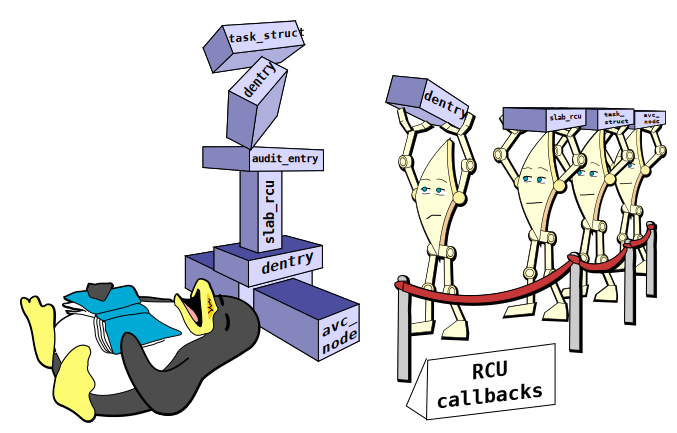
\includegraphics{cartoons/r-2014-RCU-callbacks}}
\caption{Sleeping While RCU Reading Considered Harmful}
\ContributedBy{Figure}{fig:app:rcuimpl:srcu:Sleeping While RCU Reading Considered Harmful}{Melissa Broussard}
\end{figure}

Classic RCU 는 read-side 크리티컬 섹션들이 순수한 스핀락들의 크리티컬 섹션들에
의해 지켜지는 것과 똑같은 규칙을 지킬 것을 필요로 합니다: 블락되거나 sleep
상태에 빠지는 어떠한 종류의 것들도 엄격히 금지됩니다.
이는 많은 경우 RCU 의 사용에 문제가 되었고, Paul 은 RCU read-side 크리티컬 섹션
안에서 임의적으로 잠드는 (또는 블록되는) 것을 허용하는 ``sleepable RCU'' (SRCU)
를 위한 요청을 많이 받았습니다.
Paul 은 기존에는 그런 요청들을 모두 작업할 수 없다고 거부했는데, RCU read-side
안에서 임의로 sleep 상태에 빠지는 것은 grace period 를 불명확하게 연장시킬 수
있는데, 이는 임의의 커다란 양의 메모리가 하나의 grace period 의 종료를 기다리는
결과를 초래할 것이고, 이는 결국
Figure~\ref{fig:app:rcuimpl:srcu:Sleeping While RCU Reading Considered Harmful}
에 그려진 것처럼 대부분의 경우 메모리 부족으로 인한 시스템 멎음 상태의 재앙이
되어버릴 수 있을 것이기 때문이었습니다.
무엇보다도, 시스템 멎음 상태를 초래할 수 있는---심지어 올바르게
사용되었음에도---모든 동시성 제어 기능은 존재할 가치가 없습니다.
\iffalse

Classic RCU requires that read-side critical sections
obey the same rules
obeyed by the critical sections of pure spinlocks: blocking or sleeping
of any sort is strictly prohibited.
This has frequently been an obstacle to the use of RCU, and
Paul has received numerous requests for a ``sleepable RCU'' (SRCU) that
permits arbitrary sleeping (or blocking) within RCU read-side critical
sections.
Paul had previously rejected all such requests as unworkable, since arbitrary
sleeping in RCU read-side could indefinitely extend grace periods, which
in turn could result in arbitrarily large amounts of memory awaiting the
end of a grace period, which finally would result in disaster,
as fancifully depicted in
Figure~\ref{fig:app:rcuimpl:srcu:Sleeping While RCU Reading Considered Harmful},
with the most likely disaster being hangs due to memory exhaustion.
After all, any concurrency-control primitive that could result in
system hangs---even when used correctly---does not deserve to exist.
\fi

하지만, 스핀락 크리티컬 섹션들이 preemption 될 수 있을 것을 필요로 하는
realtime 커널들~\cite{IngoMolnar05a} 또한 RCU read-side 크리티컬 섹션들이
preemption 될 수 있을 것을 필요로 했습니다~\cite{PaulMcKenney05b}.
Preemptible 크리티컬 섹션들은 데드락이 방지될 수 있도록 하기 위해
lock-acquisition 기능이 블록될 수 있을 것을 필요로 했고, 이는 곧 RCU 의, 그리고
스핀락의 크리티컬 섹션들이 락을 기다리며 블록될 수 있음을 의미하게 됩니다.
하지만, 이 두가지 형태의 sleeping 은 이 잠든 task 들을 짧은 시간 내에 깨우기
위해 사용될 수 있는 priority boosting 과 priority inheritance 라는 특수한
속성을 갖습니다.

하지만, realtime 커널들에서의 RCU 의 사용은 ``RCU read-side 크리티컬 섹션들은
결코 잠들 수 없다'' 라고 새겨져 있는 석판에 생겨난 첫번째 흠집이었습니다.
그렇다고는 하나, 들어오는 TCP 연결을 기다리면서 블록되는 것과 같은 불명확한
시간동안의 잠듦은 realtime 커널들에서조차도 엄격히 금지되어 있습니다.
\iffalse

However, the realtime kernels that require spinlock critical sections
be preemptible~\cite{IngoMolnar05a} also require that RCU read-side critical
sections be preemptible~\cite{PaulMcKenney05b}.
Preemptible critical sections in turn require that lock-acquisition
primitives block in order to avoid deadlock,
which in turns means that both RCU's and spinlocks'
critical sections be able to block awaiting a lock.
However, these two forms of sleeping have the special property that
priority boosting and priority inheritance may be used to awaken
the sleeping tasks in short order.

Nevertheless,
use of RCU in realtime kernels was the first crack in the tablets
of stone on which were inscribed ``RCU read-side critical sections can never
sleep''.
That said, indefinite sleeping, such as blocking waiting for an
incoming TCP connection, is strictly verboten even in realtime kernels.
\fi

\QuickQuiz{}
	Classic RCU read-side 크리티컬 섹션 안에서는 왜 잠드는 행위가 금지되어
	있었나요?
	\iffalse

	Why is sleeping prohibited within Classic RCU read-side
	critical sections?
	\fi
\QuickQuizAnswer{
	잠드는 행위는 Classic RCU 에서는 quiescent state 인 컨텍스트 스위치를
	암시하며, RCU 의 grace-period 탐지는 RCU read-side 크리티컬 섹션
	내에서는 quiescent state 가 결코 나타나지 말아야 할것을 필요로 하기
	때문입니다.
	\iffalse

	Because sleeping implies a context switch, which in Classic RCU is
	a quiescent state, and RCU's grace-period detection requires that
	quiescent states never appear in RCU read-side critical sections.
	\fi
} \QuickQuizEnd

\QuickQuiz{}
	quiescent state 에서 컨텍스트 스위치를 제거해버리고, user-mode 수행과
	idle loop 를 quiescent state 로 남겨둠으로써 Classic RCU read-side
	크리티컬 섹션에서의 잠드는 행위를 허용하는건 어떻습니까?
	\iffalse

	Why not permit sleeping in Classic RCU read-side critical sections
	by eliminating context switch as a quiescent state, leaving user-mode
	execution and idle loop as the remaining quiescent states?
	\fi
\QuickQuizAnswer{
	이는 상당한 kernel-mode 수행으로 이루어진 부하를 갖는 시스템 (e.x: 커널
	쓰레드로 인해) 은 grace period 의 완료를 하지 못해서 금방이든 나중이든
	메모리 부족을 일으킬 겁니다.
	\iffalse

	This would mean that a system undergoing heavy kernel-mode
	execution load (e.g., due to kernel threads) might never
	complete a grace period, which
	would cause it to exhaust memory sooner or later.
	\fi
} \QuickQuizEnd

\subsection{SRCU Implementation Strategy}
\label{sec:app:rcuimpl:SRCU Implementation Strategy}

SRC 를 설계하는데 있어서의 주요한 도전점은 RCU read-side 크리티컬 섹션 내에서
잠드는 task 가 무한히 많은 RCU callback 들을 블록 하는 것을 방지하는 것입니다.
SRCU 는 이 목표를 달성하기 위해 두개의 전략을 사용합니다:
\begin{enumerate}
\item	Classic RCU 의 \co{call_rcu()} API 와 같은 비동기적인 grace-period
	인터페이스를 제공하지 않습니다, 그리고
\item	grace-period 탐지를 각각의 SRCU 를 사용하는 subsystem 내로
	격리시킵니다.
\end{enumerate}
이런 전략들의 근본적 이유는 다음 섹션들에서 다루어집니다.
\iffalse

The primary challenge in designing an SRCU
is to prevent any given task sleeping in an RCU read-side
critical section from blocking an unbounded number of RCU callbacks.
SRCU uses two strategies to achieve this goal:
\begin{enumerate}
\item	refusing to provide asynchronous grace-period interfaces,
	such as the Classic RCU's \co{call_rcu()} API, and
\item	isolating grace-period detection within each subsystem using SRCU.
\end{enumerate}
The rationale for these strategies are discussed in the following sections.
\fi

\subsubsection{Abolish Asynchronous Grace-Period APIs}
\label{sec:app:rcuimpl:Abolish Asynchronous Grace-Period APIs}

\co{call_rcu()} API 에서의 문제는 다음에 표현된 것처럼 하나의 쓰레드가 grace
period 를 기다리는 무한히 큰 수의 메모리 블록들을 만들 수 있다는 겁니다:
\iffalse

The problem with the \co{call_rcu()} API is that a single thread can
generate an arbitrarily large number of blocks of memory awaiting a
grace period, as illustrated by the following:
\fi

\vspace{5pt}
\begin{minipage}[t]{\columnwidth}
\scriptsize
\begin{verbatim}
 1 while (p = kmalloc(sizeof(*p), GFP_ATOMIC))
 2   call_rcu(&p->rcu, f);
\end{verbatim}
\end{minipage}
\vspace{5pt}

반대로, \co{synchronize_rcu()} 를 사용하는 비슷한 코드는 쓰레드당 grace period
를 기다리는 메모리 블록은 단 하나까지만 만들 수 있습니다:
\iffalse

In contrast, the analogous code using \co{synchronize_rcu()} can
have at most a single block of memory per thread awaiting a grace period:
\fi

\vspace{5pt}
\begin{minipage}[t]{\columnwidth}
\scriptsize
\begin{verbatim}
 1 while (p = kmalloc(sizeof(*p),
 2                    GFP_ATOMIC)) {
 3   synchronize_rcu();
 4   kfree(&p->rcu, f);
 5 }
\end{verbatim}
\end{minipage}
\vspace{5pt}

따라서, SRCU 는 \co{synchronize_rcu()} 와 동일한 기능은 제공하지만
\co{call_rcu()} 에 대해서는 동일한 기능을 제공하지 않습니다.
\iffalse

Therefore, SRCU provides an equivalent to \co{synchronize_rcu()}, but not
to \co{call_rcu()}.
\fi

\subsubsection{Isolate Grace-Period Detection}
\label{sec:app:rcuimpl:Isolate Grace-Period Detection}

Classic RCU 에서는 단일 read-side 크리티컬 섹션이 무한하게 \emph{모든} RCU
callback 들을 지연시킬 수 있는데, 예를 들면 다음과 같습니다:
\iffalse

In Classic RCU, a single read-side critical section could indefinitely
delay \emph{all} RCU callbacks, for example, as follows:
\fi

\vspace{5pt}
\begin{minipage}[t]{\columnwidth}
\scriptsize
\begin{verbatim}
 1 /* BUGGY: Do not use!! */
 2 rcu_read_lock();
 3 schedule_timeout_interruptible(longdelay);
 4 rcu_read_unlock();
\end{verbatim}
\end{minipage}
\vspace{5pt}

이런 부류의 동작은 만약 RCU 가 grace period 의 긴 시간동안의 지연에도 돌아갈 수
있도록 주의깊게 설계된 하나의 subsystem 안에서만 사용되었다면 해결될 수도
있었을 겁니다.
이 긴 시간동안의 RCU read-side 지연이 사라지도록 강제한 RCU 의 \emph{모든}
사용자를 하나의 격리된 subsystem 안에서의 하나의 RCU read-side 버그가 지연시킬
수 있다는게 사실입니다.

이 문제를 우회할 수 있는 한가지 방법은 grace-period 탐지가
subsystem-by-subsystem 기반으로 이루어지도록 해서, 혼수상태의 RCU 읽기 쓰레드는
grace period 를 해당 읽기 쓰레드의 subsystem 내에서만 지연시키도록 하는
것입니다.
각각의 subsystem 은 grace period 를 기다리는 메모리 블록들을 제한된 숫자까지만
가질 수 있고, subsystem 의 수 역시 짐작건대 제한되어 있으므로, grace period 를
기다리는 메모리의 양 역시 제한될 겁니다.
특정 subsystem 의 설계자는 반드시: (1) SRCU read-side sleeping 이 제한되어
있음을 분명히 보장하고 (2) \co{synchronize_srcu()} 를 기다리는 메모리의 양을
제한해야만 합니다.\footnote{
	예를 들어, SRCU 로 보호되는 해시 테이블은 hash chain 당 하나의 락을
	가질 수 있어서, hash chain 당 최대 하나의 블록이
	\co{synchronize_srcu()} 를 기다리도록 할 수 있습니다.}

이게 정확히 SRCU 가 취한 방법으로, 다음 섹션에서 설명됩니다.
\iffalse

This sort of behavior might be tolerated if RCU were used only within
a single subsystem that was carefully designed to withstand long-term
delay of grace periods.
It is the fact that a single RCU read-side bug in one isolated subsystem can
delay \emph{all} users of RCU that forced these long-term RCU read-side
delays to be abolished.

One way around this issue is for grace-period detection to be performed
on a subsystem-by-subsystem basis, so that a lethargic RCU reader will
delay grace periods only within that reader's subsystem.
Since each subsystem can have only a bounded number of memory blocks
awaiting a grace period, and since the number of subsystems is also
presumably bounded, the total amount of memory awaiting a grace period
will also be bounded.
The designer of a given subsystem is responsible for: (1) ensuring that
SRCU read-side sleeping is bounded and (2) limiting the amount of memory
waiting for \co{synchronize_srcu()}.\footnote{
	For example, an SRCU-protected hash table might have a lock
	per hash chain, thus allowing at most one block per hash
	chain to be waiting for \co{synchronize_srcu()}.}

This is precisely the approach that SRCU takes, as described in the
following section.
\fi

\subsection{SRCU API and Usage}
\label{sec:app:rcuimpl:SRCU API and Usage}

SRCU API 가 Figure~\ref{fig:app:rcuimpl:SRCU API} 에 보여져 있습니다.
다음 섹션은 이걸 어떻게 사용하는지 설명합니다.
\iffalse

The SRCU API is shown in Figure~\ref{fig:app:rcuimpl:SRCU API}.
The following sections describe how to use it.
\fi

\begin{figure}[htbp]
{ \scriptsize
\begin{verbatim}
int init_srcu_struct(struct srcu_struct *sp);
void cleanup_srcu_struct(struct srcu_struct *sp);
int srcu_read_lock(struct srcu_struct *sp);
void srcu_read_unlock(struct srcu_struct *sp, int idx);
void synchronize_srcu(struct srcu_struct *sp);
long srcu_batches_completed(struct srcu_struct *sp);
\end{verbatim}
}
\caption{SRCU API}
\label{fig:app:rcuimpl:SRCU API}
\end{figure}

\subsubsection{Initialization and Cleanup}
\label{sec:app:rcuimpl:Initialization and Cleanup}

SRCU 를 사용하는 subsystem 각각은 \co{struct} \co{srcu_struct} 를 이 타입의
변수를 선언하는 것으로, 또는, 예를 들면 \co{kamlloc()} 등을 사용해서 동적으로
메모리를 할당하는 것으로 생성해야만 합니다.
일단 이 구조체가 만들어지면, 이 구조체는 \co{init_srcu_struct()} 로 초기화
되어야 하는데, 이 함수는 성공 시에는 0을, (예를 들어, 메모리 부족 같은 이유로
인한) 실패 시에는 에러 코드를 리턴합니다.

만약 \co{struct} \co{srcu_strcut} 가 동적으로 할당되었다면, 메모리에서 해제되기
전에 \co{cleanup_srcu_struct()} 가 반드시 호출되어야 합니다.
비슷하게, \co{struct} \co{srcu_strcut} 가 리눅스 커널 모듈 내에서 선언된
변수라면, \co{cleanup_srcu_struct()} 는 해당 모듈이 언로드 되기 전에
호출되어야만 합니다.
어떤 방식으로든, 호출자는 \co{cleanup_srcu_struct()} 의 호출 전에 모든 SRCU
read-side 크리티컬 섹션이 완료되었음을 (그리고 더이상 시작되지 않을 것을)
보장해야 합니다.
이를 달성하기 위한 방법 중 한가지가
Section~\ref{sec:app:rcuimpl:Cleaning Up Safely} 에서 설명됩니다.
\iffalse

Each subsystem using SRCU must create an
\co{struct} \co{srcu_struct},
either by declaring a variable of this type or by
dynamically allocating the memory, for example, via \co{kmalloc()}.
Once this structure is in place, it must be initialized via
\co{init_srcu_struct()}, which returns zero for success or an error
code for failure (for example, upon memory exhaustion).

If the \co{struct} \co{srcu_struct} is dynamically allocated, then
\co{cleanup_srcu_struct()} must be called before it is freed.
Similarly, if the \co{struct} \co{srcu_struct} is a variable declared within
a Linux kernel module, then \co{cleanup_srcu_struct()} must be called
before the module is unloaded.
Either way, the caller must take care to ensure that all SRCU read-side
critical sections have completed (and that no more will commence) before
calling \co{cleanup_srcu_struct()}.
One way to accomplish this is described in
Section~\ref{sec:app:rcuimpl:Cleaning Up Safely}.
\fi

\subsubsection{Read-Side Primitives}
\label{sec:app:rcuimpl:Read-Side Primitives}

The read-side \co{srcu_read_lock()} and \co{srcu_read_unlock()} primitives
are used as shown:

\vspace{5pt}
\begin{minipage}[t]{\columnwidth}
\scriptsize
\begin{verbatim}
 1 idx = srcu_read_lock(&ss);
 2 /* read-side critical section. */
 3 srcu_read_unlock(&ss, idx);
\end{verbatim}
\end{minipage}
\vspace{5pt}

The \co{ss} variable is the \co{struct} \co{srcu_struct} whose initialization
was described in Section~\ref{sec:app:rcuimpl:Initialization and Cleanup},
and the \co{idx} variable is an integer that in effect tells
\co{srcu_read_unlock()} the grace period during which the corresponding
\co{srcu_read_lock()} started.

This carrying of an index is a departure from the RCU API, which,
when required, stores the equivalent information in the task structure.
However, since a given task could potentially occupy an arbitrarily large
number of nested SRCU read-side critical sections, SRCU cannot
reasonably store this index in the task structure.

\subsubsection{Update-Side Primitives}
\label{sec:app:rcuimpl:Update-Side Primitives}

The \co{synchronize_srcu()} primitives may be used as shown below:

\vspace{5pt}
\begin{minipage}[t]{\columnwidth}
\scriptsize
\begin{verbatim}
 1 list_del_rcu(p);
 2 synchronize_srcu(&ss);
 3 kfree(p);
\end{verbatim}
\end{minipage}
\vspace{5pt}

As one might expect by analogy with Classic RCU, this primitive blocks
until until after the completion of all SRCU read-side critical sections
that started before the \co{synchronize_srcu()} started, as shown
in Table~\ref{tab:app:rcuimpl:SRCU Update and Read-Side Critical Sections}.
Here, CPU~1 need only wait for the completion of CPU~0's SRCU read-side
critical section.
It need not wait for the completion of CPU~2's SRCU read-side critical
section, because CPU~2 did not start this critical section until \emph{after}
CPU~1 began executing \co{synchronize_srcu()}.
Finally, CPU~1's \co{synchronize_srcu()} need not wait for CPU~3's
SRCU read-side critical section, because CPU~3 is using \co{s2} rather
than \co{s1} as its \co{struct} \co{srcu_struct}.
CPU~3's SRCU read-side critical section is thus related to a different
set of grace periods than those of CPUs~0 and 2.

\begin{table*}[htb]
\scriptsize
\centering
\begin{tabular}{r|l|l|l|l}
	& \multicolumn{1}{c|}{CPU 0} &
		\multicolumn{1}{c|}{CPU 1} &
			\multicolumn{1}{c|}{CPU 2} &
				\multicolumn{1}{c}{CPU 3} \\
	\hline
	\hline
	1 & \co{i0 = srcu_read_lock(&s1)} & & &
				\co{i3 = srcu_read_lock(&s2)} \\
	\hline
	2 &	& \co{synchronize_srcu(&s1)} enter & & \\
	\hline
	3 & 	&	& \co{i2 = srcu_read_lock(&s1)} & \\
	\hline
	4 & \co{srcu_read_unlock(&s1, i0)} & & & \\
	\hline
	5 &	& \co{synchronize_srcu(&s1)} exit & & \\
	\hline
	6 & 	&	 & \co{srcu_read_unlock(&s1, i2)} & \\
\end{tabular}
\caption{SRCU Update and Read-Side Critical Sections}
\label{tab:app:rcuimpl:SRCU Update and Read-Side Critical Sections}
\end{table*}

The \co{srcu_batches_completed()} primitive may be used to
monitor the progress of a given \co{struct} \co{srcu_struct}'s
grace periods.
This primitive is used in ``torture tests'' that validate SRCU's operation.

\subsubsection{Cleaning Up Safely}
\label{sec:app:rcuimpl:Cleaning Up Safely}

Cleaning up SRCU safely can be a challenge, but fortunately many
uses need not do so.
For example, uses in operating-system kernels that are initialized at
boot time need not be cleaned up.
However, uses within loadable modules must clean up if the corresponding
module is to be safely unloaded.

In some cases, such as the RCU torture module,
only a small known set of threads are using the
SRCU read-side primitives against a particular \co{struct} \co{srcu_struct}.
In these cases, the module-exit code need only kill that set of threads,
wait for them to exit, and then clean up.

In other cases, for example, for device drivers, any thread in the
system might be using the SRCU read-side primitives.
Although one could apply the method of the previous paragraph, this
ends up being equivalent to a full reboot, which can be unattractive.
Figure~\ref{fig:app:rcuimpl:SRCU Safe Cleanup} shows one way that cleanup
could be accomplished without a reboot.

\begin{figure}[htbp]
{ \scriptsize
\begin{verbatim}
  1 int readside(void)
  2 {
  3   int idx;
  4
  5   rcu_read_lock();
  6   if (nomoresrcu) {
  7     rcu_read_unlock();
  8     return -EINVAL;
  9   }
 10   idx = srcu_read_lock(&ss);
 11   rcu_read_unlock();
 12   /* SRCU read-side critical section. */
 13   srcu_read_unlock(&ss, idx);
 14   return 0;
 15 }
 16
 17 void cleanup(void)
 18 {
 19   nomoresrcu = 1;
 20   synchronize_rcu();
 21   synchronize_srcu(&ss);
 22   cleanup_srcu_struct(&ss);
 23 }
\end{verbatim}
}
\caption{SRCU Safe Cleanup}
\label{fig:app:rcuimpl:SRCU Safe Cleanup}
\end{figure}

The \co{readside()} function overlaps an RCU and an SRCU read-side
critical section, with the former running from lines~5-11 and the
latter running from lines~10-13.
The RCU read-side critical section uses Pure
%
% RCU\IfInBook{ (see Section~\ref{sec:advsync:Pure RCU})}
% 	    {~\cite{PaulEdwardMcKenneyPhD}}
%
RCU~\cite{PaulEdwardMcKenneyPhD}
%
to guard the
value of the \co{nomoresrcu} variable.
If this variable is set, we are cleaning up, and therefore must not enter
the SRCU read-side critical section, so we return \co{-EINVAL} instead.
On the other hand, if we are not yet cleaning up, we proceed into the
SRCU read-side critical section.

The \co{cleanup()} function first sets the \co{nomoresrcu} variable
on line~19, but then must wait for all currently executing RCU read-side
critical sections to complete via the \co{synchronize_rcu()} primitive
on line~20.
Once the \co{cleanup()} function reaches line~21, all calls to
\co{readside()} that could possibly have seen \co{nomorersrcu} equal
to zero must have already reached line~11, and therefore already must
have entered their SRCU read-side critical section.
All future calls to \co{readside()} will exit via line~8, and will thus
refrain from entering the read-side critical section.

Therefore, once \co{cleanup()} completes its call to
\co{synchronize_srcu()} on line~21, all SRCU read-side critical sections
will have completed, and no new ones will be able to start.
It is therefore safe on line~22 to call \co{cleanup_srcu_struct()}
to clean up.

\subsection{Implementation}
\label{sec:app:rcuimpl:Implementation}

This section describes SRCU's data structures, initialization and
cleanup primitives, read-side primitives, and update-side primitives.

\subsubsection{Data Structures}
\label{sec:app:rcuimpl:Data Structures}

SRCU's data structures are shown in
Figure~\ref{fig:app:rcuimpl:SRCU Data Structures},
and are depicted schematically in
Figure~\ref{fig:app:whymb:SRCU Data-Structure Diagram}.
The \co{completed} field is a count of the number of grace periods
since the \co{struct} \co{srcu} was initialized, and as shown in the
diagram, its low-order bit is used to index the
\co{struct} \co{srcu_struct_array}.
The \co{per_cpu_ref} field points to the array, and the
\co{mutex} field is used to permit but one \co{synchronize_srcu()} at
a time to proceed.

\begin{figure}[htbp]
{ \scriptsize
\begin{verbatim}
 1 struct srcu_struct_array {
 2   int c[2];
 3 };
 4 struct srcu_struct {
 5   int completed;
 6   struct srcu_struct_array *per_cpu_ref;
 7   struct mutex mutex;
 8 };
\end{verbatim}
}
\caption{SRCU Data Structures}
\label{fig:app:rcuimpl:SRCU Data Structures}
\end{figure}

\begin{figure}[htb]
\centering
% \resizebox{3in}{!}{\includegraphics{appendix/rcuimpl/srcuds}}
\includegraphics{appendix/rcuimpl/srcuds}
\caption{SRCU Data-Structure Diagram}
\label{fig:app:whymb:SRCU Data-Structure Diagram}
\end{figure}

\subsubsection{Initialization Implementation}
\label{sec:app:rcuimpl:Initialization Implementation}

SRCU's initialization function, \co{init_srcu_struct()}, is shown in
Figure~\ref{fig:app:rcuimpl:SRCU Initialization}.
This function simply initializes the fields in the
\co{struct} \co{srcu_struct}, returning zero if initialization succeeds
or \co{-ENOMEM} otherwise.

\begin{figure}[htbp]
{ \scriptsize
\begin{verbatim}
  1 int init_srcu_struct(struct srcu_struct *sp)
  2 {
  3   sp->completed = 0;
  4   mutex_init(&sp->mutex);
  5   sp->per_cpu_ref =
  6     alloc_percpu(struct srcu_struct_array);
  7   return (sp->per_cpu_ref ? 0 : -ENOMEM);
  8 }
\end{verbatim}
}
\caption{SRCU Initialization}
\label{fig:app:rcuimpl:SRCU Initialization}
\end{figure}

SRCU's cleanup functions are shown in
Figure~\ref{fig:app:rcuimpl:SRCU Cleanup}.
The main cleanup function, \co{cleanup_srcu_struct()} is shown
on lines~19-29 of this figure, however, it immediately invokes
\co{srcu_readers_active()}, shown on lines~13-17 of this figure,
to verify that there are no readers currently using this
\co{struct} \co{srcu_struct}.

The \co{srcu_readers_active()} function simply returns the sum of
\co{srcu_readers_active_idx()} on both possible indexes,
while \co{srcu_readers_active_idx()}, as shown on lines~1-11,
sums up the per-CPU counters corresponding to the specified index,
returning the result.

If the value returned from \co{srcu_readers_active()} is non-zero,
then \co{cleanup_srcu_struct()} issues a warning on line~24 and
simply returns on lines~25 and 26, declining to destroy a
\co{struct} \co{srcu_struct} that is still in use.
Such a warning always indicates a bug, and given that the bug
has been reported, it is better to allow the system to continue
with a modest memory leak than to introduce possible memory corruption.

Otherwise, \co{cleanup_srcu_struct()} frees the array of per-CPU
counters and \co{NULL}s the pointer on lines~27 and 28.

\begin{figure}[htbp]
{ \scriptsize
\begin{verbatim}
  1 int srcu_readers_active_idx(struct srcu_struct *sp,
  2                             int idx)
  3 {
  4   int cpu;
  5   int sum;
  6
  7   sum = 0;
  8   for_each_possible_cpu(cpu)
  9     sum += per_cpu_ptr(sp->per_cpu_ref, cpu)->c[idx];
 10   return sum;
 11 }
 12
 13 int srcu_readers_active(struct srcu_struct *sp)
 14 {
 15   return srcu_readers_active_idx(sp, 0) +
 16          srcu_readers_active_idx(sp, 1);
 17 }
 18
 19 void cleanup_srcu_struct(struct srcu_struct *sp)
 20 {
 21   int sum;
 22
 23   sum = srcu_readers_active(sp);
 24   WARN_ON(sum);
 25   if (sum != 0)
 26     return;
 27   free_percpu(sp->per_cpu_ref);
 28   sp->per_cpu_ref = NULL;
 29 }
\end{verbatim}
}
\caption{SRCU Cleanup}
\label{fig:app:rcuimpl:SRCU Cleanup}
\end{figure}

\subsubsection{Read-Side Implementation}
\label{sec:app:rcuimpl:Read-Side Implementation}

The code implementing \co{srcu_read_lock()} is shown in
Figure~\ref{fig:app:rcuimpl:Read-Side Acquisition}.
This function has been carefully constructed to avoid the
need for memory barriers and atomic instructions.

Lines~5 and 11 disable and re-enable preemption, in order to force
the sequence of code to execute unpreempted on a single CPU.
Line~6 picks up the bottom bit of the grace-period counter, which will
be used to select which rank of per-CPU counters is to be used for this
SRCU read-side critical section.
The \co{barrier()} call on line~7 is a directive to the compiler
that ensures that the index is
fetched but once,\footnote{
	Please note that, despite the name, \co{barrier()}
	has absolutely no effect on the CPU's ability to
	reorder execution of both code and of memory accesses.}
so that the index used on line~9 is the same
one returned on line~12.
Lines~8-9 increment the selected counter for the current CPU.\footnote{
	It is important to note that the \co{smp_processor_id()} primitive
	has long-term meaning only if preemption is disabled.
	In absence of preemption disabling, a potential preemption
	immediately following execution of this primitive could
	cause the subsequent code to execute on some other CPU.}
Line~10 forces subsequent execution to occur \emph{after}
lines~8-9, in order to prevent to misordering of any code
in a non-\co{CONFIG_PREEMPT} build, but only
from the perspective of an intervening interrupt handler.
However, in a \co{CONFIG_PREEMPT} kernel, the required \co{barrier()}
call is embedded in the \co{preempt_enable()} on line~11, so the
\co{srcu_barrier()} is a no-op in that case.
Finally, line~12 returns the index so that it may be passed in to the
corresponding \co{srcu_read_unlock()}.

\begin{figure}[htbp]
{ \scriptsize
\begin{verbatim}
  1 int srcu_read_lock(struct srcu_struct *sp)
  2 {
  3   int idx;
  4
  5   preempt_disable();
  6   idx = sp->completed & 0x1;
  7   barrier();
  8   per_cpu_ptr(sp->per_cpu_ref,
  9               smp_processor_id())->c[idx]++;
 10   srcu_barrier();
 11   preempt_enable();
 12   return idx;
 13 }
\end{verbatim}
}
\caption{SRCU Read-Side Acquisition}
\label{fig:app:rcuimpl:Read-Side Acquisition}
\end{figure}

The code for \co{srcu_read_unlock()} is shown in
Figure~\ref{fig:app:rcuimpl:Read-Side Release}.
Again, lines~3 and 7 disable and re-enable preemption so that the
whole code sequence executes unpreempted on a single CPU.
In \co{CONFIG_PREEMPT} kernels, the \co{preempt_disable()} on line~3
contains a \co{barrier()} primitive, otherwise, the \co{barrier()}
is supplied by line~4.
Again, this directive forces the subsequent code to execute after
the critical section from the perspective of intervening
interrupt handlers.
Lines~5 and 6 decrement the counter for this CPU, but with the same
index as was used by the corresponding \co{srcu_read_lock()}.

\begin{figure}[htbp]
{ \scriptsize
\begin{verbatim}
  1 void srcu_read_unlock(struct srcu_struct *sp, int idx)
  2 {
  3   preempt_disable();
  4   srcu_barrier();
  5   per_cpu_ptr(sp->per_cpu_ref,
  6               smp_processor_id())->c[idx]--;
  7   preempt_enable();
  8 }
\end{verbatim}
}
\caption{SRCU Read-Side Release}
\label{fig:app:rcuimpl:Read-Side Release}
\end{figure}

The key point is that a given CPU's counters
can be observed by other CPUs only in
cooperation with that CPU's interrupt handlers.
These interrupt handlers are responsible for ensuring that any needed
memory barriers are executed prior to observing the counters.

\subsubsection{Update-Side Implementation}
\label{sec:app:rcuimpl:Update-Side Implementation}

The key point behind SRCU is that \co{synchronize_sched()}
blocks until all currently-executing preempt-disabled regions of
code complete.
The \co{synchronize_srcu()} primitive makes heavy use of this effect,
as can be seen in
Figure~\ref{fig:app:rcuimpl:Update-Side Implementation}.

Line~5 takes a snapshot of the grace-period counter.
Line~6 acquires the mutex, and lines~7-10 check to see whether
at least two grace periods have elapsed since the snapshot,
and, if so, releases the lock and returns---in this case, someone
else has done our work for us.
Otherwise, line~11 guarantees that any other CPU that sees the
incremented value of the grace period counter in \co{srcu_read_lock()}
also sees any changes made by this CPU prior to entering
\co{synchronize_srcu()}.
This guarantee is required to make sure that any SRCU read-side
critical sections not blocking the next grace period have seen
any prior changes.

Line~12 fetches the bottom bit of the grace-period counter for later
use as an index into the per-CPU counter arrays, and then line~13
increments the grace-period counter.
Line~14 then waits for any currently-executing \co{srcu_read_lock()}
to complete, so that by the time that we reach line~15, all
extant instances of \co{srcu_read_lock()} will be using the updated
value from \co{sp->completed}.
Therefore, the counters sampled in by \co{srcu_readers_active_idx()}
on line~15 are guaranteed to
be monotonically decreasing, so that once their sum reaches zero, it
is guaranteed to stay there.

However, there are no memory barriers in the \co{srcu_read_unlock()}
primitive, so the CPU is within its rights to reorder the counter
decrement up into the SRCU critical section, so that references to
an SRCU-protected data structure could in effect ``bleed out'' of the
SRCU critical section.
This scenario is addressed by the \co{synchronize_sched()} on line~17,
which blocks until all other CPUs executing in \co{preempt_disable()}
code sequences (such as that in \co{srcu_read_unlock()}) complete these
sequences.
Because completion of a given \co{preempt_disable()} code sequence
is observed from the CPU executing that sequence, completion of the
sequence implies completion of any prior SRCU read-side critical section.
Any required memory barriers are supplied by the code making the
observation.

At this point, it is therefore safe to release the mutex as shown
on line~18 and return to the caller, who can now be assured that
all SRCU read-side critical sections sharing the same
\co{struct} \co{srcu_struct}
will observe any update made prior to the call to \co{synchronize_srcu()}.

\begin{figure}[htbp]
{ \scriptsize
\begin{verbatim}
  1 void synchronize_srcu(struct srcu_struct *sp)
  2 {
  3   int idx;
  4
  5   idx = sp->completed;
  6   mutex_lock(&sp->mutex);
  7   if ((sp->completed - idx) >= 2) {
  8     mutex_unlock(&sp->mutex);
  9     return;
 10   }
 11   synchronize_sched();
 12   idx = sp->completed & 0x1;
 13   sp->completed++;
 14   synchronize_sched();
 15   while (srcu_readers_active_idx(sp, idx))
 16     schedule_timeout_interruptible(1);
 17   synchronize_sched();
 18   mutex_unlock(&sp->mutex);
 19 }
\end{verbatim}
}
\caption{SRCU Update-Side Implementation}
\label{fig:app:rcuimpl:Update-Side Implementation}
\end{figure}

\QuickQuiz{}
	Why is it OK to assume that updates separated by
	\co{synchronize_sched()} will be performed in order?
\QuickQuizAnswer{
	Because this property is required for the \co{synchronize_sched()}
	aspect of RCU to work at all.
	For example, consider a code sequence that removes an object
	from a list, invokes \co{synchronize_sched()}, then frees
	the object.
	If this property did not hold, then that object might appear
	to be freed before it was
	removed from the list, which is precisely the situation that
	\co{synchronize_sched()} is supposed to prevent!
} \QuickQuizEnd

\QuickQuiz{}
	Why must line~17 in \co{synchronize_srcu()}
	(Figure~\ref{fig:app:rcuimpl:Update-Side Implementation})
	precede the release of the mutex on line~18?
	What would have to change to permit these two lines to be
	interchanged?
	Would such a change be worthwhile?
	Why or why not?
\QuickQuizAnswer{
	Suppose that the order was reversed, and that CPU~0
	has just reached line~13 of
	\co{synchronize_srcu()}, while both CPU~1 and CPU~2 start executing
	another \co{synchronize_srcu()} each, and CPU~3 starts executing a
	\co{srcu_read_lock()}.
	Suppose that CPU~1 reaches line~6 of \co{synchronize_srcu()}
	just before CPU~0 increments the counter on line~13.
	Most importantly, suppose that
	CPU~3 executes \co{srcu_read_lock()}
	out of order with the following SRCU read-side critical section,
	so that it acquires a reference to some SRCU-protected data
	structure \emph{before} CPU~0 increments \co{sp->completed}, but
	executes the \co{srcu_read_lock()} \emph{after} CPU~0 does
	this increment.
	
	Then CPU~0 will \emph{not} wait for CPU~3 to complete its
	SRCU read-side critical section before exiting the ``while''
	loop on lines~15-16 and releasing the mutex (remember, the
	CPU could be reordering the code).
	
	Now suppose that CPU~2 acquires the mutex next,
	and again increments \co{sp->completed}.
	This CPU will then have to wait for CPU~3 to exit its SRCU
	read-side critical section before exiting the loop on
	lines~15-16 and releasing the mutex.
	But suppose that CPU~3 again executes out of order,
	completing the \co{srcu_read_unlock()} prior to
	executing a final reference to the pointer it obtained
	when entering the SRCU read-side critical section.

	CPU~1 will then acquire the mutex, but see that the
	\co{sp->completed} counter has incremented twice, and
	therefore take the early exit.
	The caller might well free up the element that CPU~3 is
	still referencing (due to CPU~3's out-of-order execution).

	To prevent this perhaps improbable, but entirely possible,
	scenario, the final \co{synchronize_sched()} must precede
	the mutex release in \co{synchronize_srcu()}.

	Another approach would be to change to comparison on
	line~7 of \co{synchronize_srcu()} to check for at
	least three increments of the counter.
	However, such a change would increase the latency of a
	``bulk update'' scenario, where a hash table is being updated
	or unloaded using multiple threads.
	In the current code, the latency of the resulting concurrent
	\co{synchronize_srcu()} calls would take at most two SRCU
	grace periods, while with this change, three would be required.

	More experience will be required to determine which approach
	is really better.
	For one thing, there must first be some use of SRCU with
	multiple concurrent updaters.
} \QuickQuizEnd

\subsection{SRCU Summary}
\label{sec:app:rcuimpl:SRCU Summary}

SRCU provides an RCU-like set of primitives that permit general
sleeping in the SRCU read-side critical sections.
However, it is important to note that SRCU has been used only in
prototype code, though it has passed the RCU torture test.
It will be very interesting to see what use, if any, SRCU sees
in the future.

% \input{appendix/rcuimpl/rcuclassic.tex}  @@@ from Ph.D. dissertation.
% appendix/rcuimpl/rcutree.tex

\section{Hierarchical RCU Overview}
\label{app:rcuimpl:rcutree:Hierarchical RCU Overview}
\OriginallyPublished{Appendix}{app:rcuimpl:rcutree:Hierarchical RCU Overview}{Hierarchical RCU Overview}{Linux Weekly News}{PaulEMcKenney2008HierarchicalRCU}

Classic RCU 의 read-side 기능들은 훌륭한 성능과 확장성을 갖긴 합니다만, 언제
이전부터 존재한 read-side 크리티컬 섹션들이 완료되었는지를 결정하는데 사용되는
update-side 기능들은 수십개의 CPU 들만을 고려한 채 설계되었습니다.
이것들의 확장성은 각 grace period 마다 최소 한번은 각 CPU 에 의해 획득되어야
하는 global lock 에 의해 제한됩니다.
Classic RCU 는 실제로는 수백개의 CPU 들까지도 확장성을 갖고, 대략 천개의 CPU
들까지도 확장성을 갖도록 (더 길어지는 grace period 를 대가로) 꼼수를 부릴 수
있지만, 발전되는 중인 멀티코어 시스템들은 더 높은 확장성을 필요로 할겁니다.
\iffalse

Although Classic RCU's read-side primitives enjoy excellent
performance and scalability, the update-side primitives, which
determine when pre-existing read-side critical sections have
finished, were designed with only a few tens of CPUs in mind.
Their scalability is limited by a global lock that must be
acquired by each CPU at least once during each grace period.
Although Classic RCU actually scales to a couple of hundred CPUs, and
can be tweaked to scale to roughly a thousand CPUs (but at the expense of
extending grace periods), emerging multicore systems will require
it to scale better.
\fi

또한, Classic RCU 는 최적화 되지 않은 dynticks 인터페이스를 가지고 있어서,
Classic RCU 는 매 grace period 마다 최소 한번씩은 깨어나게 할겁니다.
이 문제를 자세히 보려면, 4개의 CPU 만이 바쁘게 유지되고 있을 정도로 적은
부하만을 가지고 있는 16-CPU 시스템을 생각해 보세요.
완벽한 세계에서는, 나머지 열두개의 CPU 들은 에너지를 아끼기 위해 깊은 sleep
모드로 빠져있을 수 있을 겁니다.
불행히도, 네개의 바쁜 CPU 들이 자주 RCU update 동작을 수행한다면, 이 열두개의
idle CPU 들은 자주 깨어나서 상당한 전력을 소모할 겁니다.
따라서, Classic RCU 에의 주요 변경 사항들은 항상 잠들어있는 CPU 들을 놔두어야
합니다.
\iffalse

In addition, Classic RCU has a sub-optimal dynticks interface,
with the result that Classic RCU will wake up every CPU at least
once per grace period.
To see the problem with this, consider a 16-CPU system that
is sufficiently lightly loaded that it is keeping only four
CPUs busy.
In a perfect world, the remaining twelve CPUs could be put into
deep sleep mode in order to conserve energy.
Unfortunately, if the four busy CPUs are frequently performing
RCU updates, those twelve idle CPUs will be awakened frequently,
wasting significant energy.
Thus, any major change to Classic RCU should also leave sleeping CPUs lie.
\fi

Classic 과 hierarchical 구현들 둘 다 Classic RCU 의 semantic 과 동일한 API 들을
가지고 있습니다만, 기존의 구현은 ``classic RCU'' 로 불리울 것이고, 새로운
구현은 ``hierarchical RCU'' 라 불릴 겁니다.
\iffalse

Both the classic and the hierarchical implementations
have Classic RCU semantics and identical APIs, however,
the old implementation will be called ``classic RCU''
and the new implementation will be called ``hierarchical RCU''.
\fi

Section~\ref{app:rcuimpl:rcutree:Review of RCU Fundamentals}
은 RCU 의 기본에 대한 짧은 개괄을 제공하고
Section~\ref{app:rcuimpl:rcutree:Brief Overview of Classic RCU Implementation}
은 기존의 ``Classic RCU'' 구현에 대한 전반적인 개괄을 제공합니다.
Section~\ref{app:rcuimpl:rcutree:RCU Desiderata}
은 RCU 에서 일어나지 않을 것 같은 일들을 나열해보고,
Section~\ref{app:rcuimpl:rcutree:Towards a More Scalable RCU Implementation}
과~\ref{app:rcuimpl:rcutree:Towards a Greener RCU Implementation}
에서는 확장성과 전력 효율성을 위한 설계상의 고려할 점들을 각각 알아보고,
Section~\ref{app:rcuimpl:rcutree:State Machine}
에서 hierarchical RCU state machine 을 설명합니다.
Section~\ref{app:rcuimpl:rcutree:Use Cases},
Section~\ref{app:rcuimpl:rcutree:Testing}
는 테스트를 다루고, 마지막으로
Section~\ref{app:rcuimpl:rcutree:Conclusion}
에서 결론을 내립니다.
\iffalse

Section~\ref{app:rcuimpl:rcutree:Review of RCU Fundamentals}
gives a brief review of RCU fundamentals and
Section~\ref{app:rcuimpl:rcutree:Brief Overview of Classic RCU Implementation}
gives a brief overview of the old ``Classic RCU'' implementation.
Section~\ref{app:rcuimpl:rcutree:RCU Desiderata}
lists RCU desiderata,
Sections~\ref{app:rcuimpl:rcutree:Towards a More Scalable RCU Implementation}
and~\ref{app:rcuimpl:rcutree:Towards a Greener RCU Implementation}
lay out design considerations for scalability and energy efficiency,
respectively, and
Section~\ref{app:rcuimpl:rcutree:State Machine}
describes the hierarchical RCU state machine.
Section~\ref{app:rcuimpl:rcutree:Use Cases},
Section~\ref{app:rcuimpl:rcutree:Testing}
covers testing, and finally,
Section~\ref{app:rcuimpl:rcutree:Conclusion}
presents concluding remarks.
\fi

\subsection{Review of RCU Fundamentals}
\label{app:rcuimpl:rcutree:Review of RCU Fundamentals}

가장 기본적 형태에 있어, RCU 는 일이 끝나길 기다리는 방법입니다.
물론, 일이 끝나길 기다리는 방법은 레퍼런스 카운트, reader-writer 락, 이벤트,
등등 매우 많이 존재합니다.
RCU 의 커다란 장점은 (대략) 20,000 개의 서로 다른 일들을 명시적으로 하나하나 다
정보를 추적할 필요 없이, 그리고 명시적 추적에서는 피할 수 없는 성능의 하락,
확장성의 제약, 복잡한 데드락 시나리오, 메모리 누수 문제 없이 각각 기다릴 수
있다는 겁니다.
\iffalse

In its most basic form, RCU is a way of waiting for things to finish.
Of course, there are a great many other ways of waiting for things to
finish, including reference counts, reader-writer locks, events, and so on.
The great advantage of RCU is that it can wait for each of
(say) 20,000 different things without having to explicitly
track each and every one of them, and without having to worry about
the performance degradation, scalability limitations, complex deadlock
scenarios, and memory-leak hazards that are inherent in schemes
using explicit tracking.
\fi

RCU 의 경우, 기다리는 것들은 ``RCU read-side 크리티컬 섹션'' 이라 불리웁니다.
하나의 RCU read-side 크리티컬 섹션은 \co{rcu_read_lock()} 기능으로 시작하고,
연관된 \co{rcu_read_unlock()} 기능으로 종료됩니다.
RCU read-side 크리티컬 섹션들은 중첩될 수 있고, 명시적으로 블록되거나 잠들지
않는다면, 상당히 많은 양의 임의적 코드를 포함할 수 있습니다 (
Section~\ref{app:rcuimpl:Sleepable RCU Implementation} 에서 설명한 SRCU 라
불리는 특수한 형태의 RCU 는 SRCU read-side 크리티컬 섹션 내에서의 일반적인
sleeping 을 허용하긴 하지만요).
여러분이 이러한 표준을 준수한다면, 여러분은 \emph{모든} 코드 조각에 대해
완료되길 기다리는데에 RCU 를 사용할 수 있습니다.

RCU 는 언제 이것들이 끝나는지를 간접적으로 판단함으로써 이 기능을 구현하는데,
classic RCU 의 경우 다른 곳~\cite{McKenney98} 에서, preemptible RCU 의 경우
Section~\ref{app:rcuimpl:Preemptible RCU} 에서 자세히 설명합니다.
\iffalse

In RCU's case, the things waited on are called
``RCU read-side critical sections''.
An RCU read-side critical section starts with an
\co{rcu_read_lock()} primitive, and ends with a corresponding
\co{rcu_read_unlock()} primitive.
RCU read-side critical sections can be nested, and may contain pretty
much any code, as long as that code does not explicitly block or sleep
(although a special form of RCU called SRCU, described in
Section~\ref{app:rcuimpl:Sleepable RCU Implementation}
does permit general sleeping in SRCU read-side critical sections).
If you abide by these conventions, you can use RCU to wait for \emph{any}
desired piece of code to complete.

RCU accomplishes this feat by indirectly determining when these
other things have finished, as has been described
elsewhere~\cite{McKenney98}
for classic RCU and
Section~\ref{app:rcuimpl:Preemptible RCU} for preemptible RCU.
\fi

자세히 말하자면,
page~\pageref{fig:defer:Readers and RCU Grace Period} 의
Figure~\ref{fig:defer:Readers and RCU Grace Period} 에서 보인 바와 같이, RCU 는
앞서 존재하기 시작한 RCU read-side 크리티컬 섹션들과 그것들에 의해 수행된
메모리 오퍼레이션들이 완전히 종료되기를 기다리는 방법입니다.

하지만, 특정 grace period 가 시작한 후에 시작된 RCU read-side 크리티컬 섹션들은
해당 grace period 종료 뒤까지도 연장될 수 있음을 알아두시기 바랍니다.

다음 섹션은 Classic RCU 구현이 어떻게 동작하는지에 대한 높은 수준에서의 개관을
제공합니다.
\iffalse

In particular, as shown in the
Figure~\ref{fig:defer:Readers and RCU Grace Period} on
page~\pageref{fig:defer:Readers and RCU Grace Period},
RCU is a way of
waiting for pre-existing RCU read-side critical sections to completely
finish, also including the memory operations executed
by those critical sections.

However, note that RCU read-side critical sections
that begin after the beginning
of a given grace period can and will extend beyond the end of that grace
period.

The following section gives a very high-level view of how
the Classic RCU implementation operates.
\fi

\subsection{Brief Overview of Classic RCU Implementation}
\label{app:rcuimpl:rcutree:Brief Overview of Classic RCU Implementation}

Classic RCU 구현 아래의 핵심 컨셉은, Classic RCU read-side 크리티컬 섹션은 커널
코드에 국한되어 있고 블록이 허용되어있지 않다는 것입니다.
이말은 언제든 어떤 CPU 가 블록되어 있는 중으로 보이거나, idle loop 을 돌고
있거나, 커널 모드를 빠져나가 있다면, 우리는 해당 CPU 에서 앞서 수행중이던 RCU
read-side 크리티컬 섹션이 모두 완료되었어야 함을 알 수 있다는 것입니다.
그런 상태는 ``quiescent states'' 라 불리며, 각각의 CPU 가 적어도 하나의
quiscent state 를 거쳤다면, 해당 RCU grace period 는 끝납니다.
\iffalse

The key concept behind the Classic RCU implementation is that
Classic RCU read-side critical sections are confined to kernel
code and are not permitted to block.
This means that any time a given CPU is seen
either blocking, in the idle loop, or exiting the kernel, we know that all
RCU read-side critical sections that were previously running on
that CPU must have completed.
Such states are called ``quiescent states'', and
after each CPU has passed through at least one quiescent state,
the RCU grace period ends.
\fi

\begin{figure}[htb]
\centering
\resizebox{3in}{!}{\includegraphics{appendix/rcuimpl/FlatClassicRCU}}
\caption{Flat Classic RCU State}
\label{fig:app:rcuimpl:rcutree:Flat Classic RCU State}
\end{figure}

Classic RCU 의 가장 중요한 데이터 구조는 \co{rcu_ctrlblk} 구조체로,
Figure~\ref{fig:app:rcuimpl:rcutree:Flat Classic RCU State} 에 보인 것처럼 CPU
당 하나의 bit 을 담고 있는 \co{->cpumask} 필드를 가지고 있습니다.
각각의 CPU 의 bit 은 각각의 grace period 의 시작지점에서 1로 설정되고, 각각의
CPU 는 quiescent state 를 지날 때마다 자신의 bit 의 값을 해제합니다.
여러개의 CPU 들이 각자의 bit 을 동시적으로 값 해제하고자 할 수 있으며 이는
\co{->cpumask} 필드를 오염시킬 수 있기 때문에, 그런 문제를 방지하기 위해
\co{->cpumask} 필드를 보호하는데에 \co{->lock} 스핀락이 사용됩니다.
안타깝게도, 멀티코어 트렌드가 지속된다면 곧 흔한 경우가 될 수백개가 넘는 CPU 가
존재한다면 이 스핀락 또한 상당한 경쟁상태로 성능에 악영향을 줄 수 있습니다.
더 나쁜건, \emph{모든} CPU 들이 각자의 bit 을 값 해제해야 한다는 사실은 CPU
들이 grace period 동안은 잠들지 않아야 함을 말하는데, 이는 Linux 의 전력 소모
감소 능력이 제한됨을 말합니다.

다음 섹션은 새로운 real-time 이 아닌 RCU 구현에서 필요한 것들을 나열합니다.
\iffalse

Classic RCU's most important data structure is the \co{rcu_ctrlblk}
structure, which contains the \co{->cpumask} field, which contains
one bit per CPU, as shown in
Figure~\ref{fig:app:rcuimpl:rcutree:Flat Classic RCU State}.
Each CPU's bit is set to one at the beginning of each grace period,
and each CPU must clear its bit after it passes through a quiescent
state.
Because multiple CPUs might want to clear their bits concurrently,
which would corrupt the \co{->cpumask} field, a
\co{->lock}
spinlock is used to protect \co{->cpumask}, preventing any
such corruption.
Unfortunately, this spinlock can also suffer extreme contention if there
are more than a few hundred CPUs, which might soon become quite common
if multicore trends continue.
Worse yet, the fact that \emph{all} CPUs must clear their own bit means
that CPUs are not permitted to sleep through a grace period, which limits
Linux's ability to conserve power.




The next section lays out what we need from a new non-real-time
RCU implementation.
\fi

\subsection{RCU Desiderata}
\label{app:rcuimpl:rcutree:RCU Desiderata}

Real-time RCU 의 요구사항~\cite{PaulMcKenney05b} 을 나열해 보는게 좋은 시작점이
될겁니다:
\iffalse

The list of real-time RCU desiderata~\cite{PaulMcKenney05b}
is a very good start:
\fi

\begin{enumerate}
\item	하나의 RCU grace period 는 모든 이전부터 존재한 RCU read-side 크리티컬
	섹션들이 완료될 때까지 끝날 수 없도록 하는 지연된 해체.
\item	일년 365일 24시간 지속되는 동작을 지원할 수 있는 신뢰성.
\item	Irq 핸들러에서 호출할 수 있을 것.
\item	너무 많은 콜백들이 존재한다면 grace period 들을 신속히 처리할 수 있는
	메커니즘이 존재할 수 있도록 하는, 억제된 메모리 사용량 (LCA2005
	리스트로 효력이 약화되었습니다.)
\item	RCU 가 어떤 있음직한 메모리 할당자와도 동작할 수 있도록 해주는 메모리
	블락들의 독립성.
\item	CPU 나 태스크의 지역적 메모리 에서의 평범한, 어토믹하지 않은 인스트럭션
	동작이 허용될 수 있도록 하는 동기화에 자유로운 read side (이건 LCA2005
	리스트에서 강화되었습니다.).
\item	Update-side 락이 RCU read-side 크리티컬 섹션 내에서 획득되어지는,
	리눅스 커널의 여러곳에서 사용되는 무조건적인 read-to-write 업그레이드.
\item	호환성 있는 API.
\iffalse

\item	Deferred destruction, so that an RCU grace period cannot end
	until all pre-existing RCU read-side critical sections have
	completed.
\item	Reliable, so that RCU supports 24x7 operation for years at
	a time.
\item	Callable from irq handlers.
\item	Contained memory footprint, so that mechanisms exist to expedite
	grace periods if there are too many callbacks.  (This is weakened
	from the LCA2005 list.)
\item	Independent of memory blocks, so that RCU can work with any
	conceivable memory allocator.
\item	Synchronization-free read side, so that only normal non-atomic
	instructions operating on CPU- or task-local memory are permitted.
	(This is strengthened from the LCA2005 list.)
\item	Unconditional read-to-write upgrade, which is used in several
	places in the Linux kernel where the update-side lock is
	acquired within the RCU read-side critical section.
\item	Compatible API.
\fi

\item	이건 real-time RCU 가 될 것은 아니기에, preemption 가능한 RCU read-side
	크리티컬 섹션에 대한 요구사항은 빠졌습니다.
	하지만, 과거 수년동안의 변경사항들을 처리하기 위해 다음의 새로운
	요구사항들을 추가할 필요가 있습니다.

\item	극단적으로 낮은 internal-to-RCU 락 경쟁상황을 갖는 확장성.
	RCU 는 최소 1,024 개, 가능하면 최소 4,096 개의 CPU 들을 지원해야
	합니다.
\item	전력 효율성: RCU 는 저전력 상태의 dynticks-idle CPU 들을 깨우지
	않으면서도 언제 현재의 grace period 가 종료되는지를 알 수 있어야
	합니다.
	이는 real-time RCU 에서 구현되었습니다만, 상당한 단순화를 필요로
	합니다.
\item	RCU read-side 크리티컬 섹션들은 irq 핸들러는 물론이고 NMI 핸들러
	내에서도 사용이 가능해야 합니다.  Preemptible RCU 의 경우에는 별도로
	구현된 \co{synchronize_sched()} 덕분에 이 필요성이 없었음을 알아두시기
	바랍니다.
\item	RCU 는 반복되는 CPU-hotplug 오퍼레이션들의 상황에서도 잘 동작해야
	합니다.
	이는 classic RCU 와 real-time RCU 에서의 필요사항들을 가져올 뿐입니다.
\item	앞서 등록된 모든 RCU 콜백들이 완료되길 기다릴 수 있어야만 하는데, 이는
	이미 \co{rcu_barrier()} 의 형태로 제공되긴 합니다.
\iffalse

\item	Because this is not to be a real-time RCU, the requirement for
	preemptible RCU read-side critical sections can be dropped.
	However, we need to add the following new requirements to account
	for changes over the past few years.

\item	Scalability with extremely low internal-to-RCU lock contention.
	RCU must support at least 1,024 CPUs gracefully, and preferably
	at least 4,096.
\item	Energy conservation: RCU must be able to avoid awakening
	low-power-state dynticks-idle CPUs, but still determine
	when the current grace period ends.
	This has been implemented in real-time RCU, but needs serious
	simplification.
\item	RCU read-side critical sections must be permitted in NMI
	handlers as well as irq handlers.  Note that preemptible RCU
	was able to avoid this requirement due to a separately
	implemented \co{synchronize_sched()}.
\item	RCU must operate gracefully in face of repeated CPU-hotplug
	operations.
	This is simply carrying forward a requirement met by both
	classic and real-time.
\item	It must be possible to wait for all previously registered
	RCU callbacks to complete, though this is already provided
	in the form of \co{rcu_barrier()}.
\fi
\item	RCU 와 다양한 무한 루프 버그들, 그리고 RCU grace period 가 종료되기를
	막는 하드웨어 상의 문제들을 진단하는데 도움이 될 수 있도록, 응답을
	하는데 실패하는 CPU 들을 파악할 수 있다면 좋습니다.
\item	하나의 RCU grace period 가 마지막 연관된 RCU read-side 크리티컬 섹션이
	완료되는데에 수백 마이크로세컨드 만이 걸릴 수 있도록 하는 RCU grace
	period 의 극단적인 속도 촉진이 가능하면 좋습니다.
	하지만, 그런 동작은 상당한 CPU 오버헤드를 가져올 거라 예상되어지며,
	각각이 RCU grace period 를 기다려야 하는 긴 일련의 오퍼레이션들을
	처리해야 할때 유용할 겁니다.
\iffalse

\item	Detecting CPUs that are failing to respond is desirable,
	to assist diagnosis both of RCU and of various infinite
	loop bugs and hardware failures that can prevent RCU grace
	periods from ending.
\item	Extreme expediting of RCU grace periods is desirable,
	so that an RCU grace period can be forced to complete within
	a few hundred microseconds of the last relevant RCU read-side
	critical second completing.
	However, such an operation would be expected to incur
	severe CPU overhead, and would be primarily useful when
	carrying out a long sequence of operations that each needed
	to wait for an RCU grace period.
\fi
\end{enumerate}

새로운 효구사항들 가운데 가장 압박이 되는건 첫번째 항목인 확장성입니다.
따라서 다음 섹션은 RCU 의 내부 락들의 경쟁 상황을 수십배 줄여주는지 설명합니다.
\iffalse

The most pressing of the new requirements is the first one, scalability.
The next section therefore describes how to make order-of-magnitude reductions
in contention on RCU's internal locks.
\fi

\subsection{Towards a More Scalable RCU Implementation}
\label{app:rcuimpl:rcutree:Towards a More Scalable RCU Implementation}

\begin{figure}[htb]
\centering
\resizebox{3in}{!}{\includegraphics{appendix/rcuimpl/TreeClassicRCU}}
\caption{Hierarchical RCU State}
\label{fig:app:rcuimpl:rcutree:Hierarchical RCU State}
\end{figure}

락 경쟁을 줄여주는 효과적인 방법 가운데 하나는
Figure~\ref{fig:app:rcuimpl:rcutree:Hierarchical RCU State} 에 보인 것처럼
계층을 만드는 것입니다.
여기서, 각각의 네개의 \co{rcu_node} 구조체는 자신의 락을 가지고 있어서, CPU~0
과 1 만이 좌하단의 \co{rcu_node} 의 락을 획득하며, CPU~2 와 3 만이 중하단의
\co{rcu_node} 의 락을 획득하고, CPU~4 와 5 만이 우하단의 \co{rcu_node} 의 락을
획득합니다.
어떤 특정 grace period 동안에도, 아래쪽 \co{rcu_node} 구조체들에 접근하는 CPU
들 가운데 하나만이 위의 \co{rcu_node} 에 접근하게 되어서, 각각의 CPU 짝 들
가운데 마지막 하나만이 연관된 grace period 에 대한 quiescent state 를 기록하게
됩니다.

이는 락 경쟁의 상당한 감소를 초래합니다:
여섯개의 CPU 들이 하나의 락을 위해 매 grace period 마다 경쟁하는 대신, 위쪽
\co{rcu_node} 락에 세개의 CPU 만이 경쟁하고 (50\% 경쟁 감소) 아래쪽
\co{rcu_node} 의 락에 대해서는 각각 두개의 CPU 만이 경쟁을 합니다 (67\% 경쟁
감소).
\iffalse

One effective way to reduce lock contention is to create a hierarchy,
as shown in
Figure~\ref{fig:app:rcuimpl:rcutree:Hierarchical RCU State}.
Here, each of the four \co{rcu_node} structures has its own lock,
so that only CPUs~0 and 1 will acquire the lower left
\co{rcu_node}'s lock, only CPUs~2 and 3 will acquire the
lower middle \co{rcu_node}'s lock, and only CPUs~4 and 5
will acquire the lower right \co{rcu_node}'s lock.
During any given grace period,
only one of the CPUs accessing each of the lower \co{rcu_node}
structures will access the upper \co{rcu_node}, namely, the
last of each pair of CPUs to record a quiescent state for the corresponding
grace period.

This results in a significant reduction in lock contention:
instead of six CPUs contending for a single lock each grace period,
we have only three for the upper \co{rcu_node}'s lock
(a reduction of 50\%) and only
two for each of the lower \co{rcu_node}s' locks (a reduction
of 67\%).
\fi

\begin{figure}[htb]
\centering
\resizebox{3in}{!}{\includegraphics{appendix/rcuimpl/TreeMapping}}
\caption{Mapping {\tt rcu\_node} Hierarchy Into Array}
\label{fig:app:rcuimpl:rcutree:Mapping rcu-node Hierarchy Into Array}
\end{figure}

\co{rcu_node} 구조체들의 트리는 \co{rcu_state} 구조체 안의 선형적 배열로 트리의
루트를 0번 원소로 저장하는 식으로 내장되는데,
Figure~\ref{fig:app:rcuimpl:rcutree:Mapping rcu-node Hierarchy Into Array} 에
여덟개의 CPU 를 갖는 시스템에서 세 단계를 갖는 계층으로 구성했을 때를 보이고
있습니다.
각각의 화살표는 특정 \co{rcu_node} 구조체를 그 부모로 연결시키는데,
\co{rcu_node} 의 \co{->parent}  필드를 나타냅니다.
각각의 \co{rcu_node} 는 자신이 관리하는 CPU 들의 범위를 나타내는데, 루트 노드는
모든 CPU 들을 관리하고, leaf 레벨의 각각의 노드는 한쌍의 CPU 들을 관리합니다.
이 배열은 컴파일 시점에 \co{NR_CPUS} 값에 따라 정적으로 할당됩니다.
\iffalse

The tree of \co{rcu_node} structures is embedded into
a linear array in the \co{rcu_state} structure,
with the root of the tree in element zero, as shown in
Figure~\ref{fig:app:rcuimpl:rcutree:Mapping rcu-node Hierarchy Into Array}
for an eight-CPU
system with a three-level hierarchy.
Each arrow links a given \co{rcu_node} structure to its parent,
representing the \co{rcu_node}'s \co{->parent} field.
Each \co{rcu_node} indicates the range of CPUs covered,
so that the root node covers all of the CPUs, each node in the second
level covers half of the CPUs, and each node in the leaf level covering
a pair of CPUs.
This array is allocated statically at compile time based on the value
of \co{NR_CPUS}.
\fi

\begin{figure}[htbp]
\centering
\resizebox{3in}{!}{\includegraphics{appendix/rcuimpl/TreeClassicRCUGP}}
\caption{Hierarchical RCU Grace Period}
\label{fig:app:rcuimpl:rcutree:Hierarchical RCU Grace Period}
\end{figure}

Figure~\ref{fig:app:rcuimpl:rcutree:Hierarchical RCU Grace Period}
안의 다이어그램들의 시퀀스는 어떻게 grace period 들이 파악되는지를 보입니다.
첫번째 그림에서는 어떤 CPU 도 빨간 네모로 표시되었듯이 quiescent state 에
이르지 못했습니다.
모든 여섯개의 CPU 들이 동시에 RCU 에게 자신이 quiescent state 에 이르렀노라고
이야기하고자 한다고 생각해 봅시다.
각각의 쌍 안의 CPU 들 중 하나만이 연관된 아래쪽 \co{rcu_node} 의 락을 획득할 수
있을 것이고, 따라서 두번째 그림은 그런 운좋은 CPU 들이 0, 3, 그리고 5 라고
초록색 네모로 나타내고 있습니다.
이 운좋은 CPU 들이 일단 마무리 되면, 다른 CPU 들이 락을 획득할 것인데, 세번째
그림으로 보인 바와 같습니다.
이 CPU 들 각각은 자신들이 자신의 그룹 내에서는 마지막에 이르렀음을 보게 되고,
따라서 모든 세개의 CPU 들은 위쪽의 \co{rcu_node} 로 이동하려 시도하게 됩니다.
한번에 하나만이 위쪽 \co{rcu_node} 구조체의 락을 얻을 수 있고, 네번째,
다섯번째, 그리고 여섯번째 그림은 CPU~1, CPU~2, 그리고 CPU~4 가 순서대로 그 락을
잡는다는 가정 하에 상태의 흐름을 보입니다.
마지막 여섯번째 그림은 모든 CPU 들이 quiescent state 를 지난, 그래서 grace
period 가 끝난 경우를 보이고 있습니다.
\iffalse

The sequence of diagrams in
Figure~\ref{fig:app:rcuimpl:rcutree:Hierarchical RCU Grace Period}
shows how grace periods are detected.
In the first figure, no CPU has yet passed through a quiescent state,
as indicated by the red rectangles.
Suppose that all six CPUs simultaneously try to tell RCU that they have
passed through a quiescent state.
Only one of each pair will be able to acquire the lock on the
corresponding lower \co{rcu_node}, and so the second figure
shows the result if the lucky CPUs are numbers 0, 3, and 5, as indicated
by the green rectangles.
Once these lucky CPUs have finished, then the other CPUs will acquire
the lock, as shown in the third figure.
Each of these CPUs will see that they are the last in their group,
and therefore all three will attempt to move to the upper
\co{rcu_node}.
Only one at a time can acquire the upper \co{rcu_node} structure's
lock, and the fourth, fifth, and sixth figures show the sequence of
states assuming that CPU~1, CPU~2, and CPU~4 acquire
the lock in that order.
The sixth and final figure in the group shows that all CPUs have passed
through a quiescent state, so that the grace period has ended.
\fi

\begin{figure}[htb]
\centering
\resizebox{3in}{!}{\includegraphics{appendix/rcuimpl/BigTreeClassicRCU}}
\caption{Hierarchical RCU State 4,096 CPUs}
\label{fig:app:rcuimpl:rcutree:Hierarchical RCU State 4,096 CPUs}
\end{figure}

앞의 예에서, Classic RCU 에서라면 여섯개의 CPU 들이 경쟁하게 될 터인 것을 어떤
하나의 락에 대해서는 세개가 넘는 CPU 들이 경쟁하지 않았습니다.
하지만, 더 많은 수의 CPU 들에서라면 이보다도 극적인 락 경쟁의 감소가
가능합니다.
64 개의 아래쪽 구조체와 64*64=4,096 CPU 들로 구성된,
Figure~\ref{fig:app:rcuimpl:rcutree:Hierarchical RCU State 4,096 CPUs} 에 보인
것과 같은 \co{rcu_node} 구조체들의 계층을 생각해 보세요.

여기서 각각의 아래쪽 \co{rcu_node} 구조체의 락들은 64 개의 CPU 들에 의해
획득되어지는데, 이는 Classic RCU 의 하나의 글로벌 락에 4,096 개의 CPU 들이
경쟁하는 것에 비해 64배의 감소입니다.
비슷하게, 특정 grace period 동안에, 아래쪽 \co{rcu_node} 구조체의 CPU 들 가운데
하나만이 위쪽 \co{rcu_node} 구조체의 락을 잡을 것이므로, 이는 또다시 4,096 개의
CPU 로 구성된 시스템에서 동작하는 Classic RCU 가 겪게 되는 경쟁의 64x
감소입니다.
\iffalse

In the above sequence, there were never more than three CPUs
contending for any one lock, in happy contrast to Classic RCU,
where all six CPUs might contend.
However, even more dramatic reductions in lock contention are
possible with larger numbers of CPUs.
Consider a hierarchy of \co{rcu_node} structures, with
64 lower structures and 64*64=4,096 CPUs, as shown in
Figure~\ref{fig:app:rcuimpl:rcutree:Hierarchical RCU State 4,096 CPUs}.

Here each of the lower \co{rcu_node} structures' locks
are acquired by 64 CPUs, a 64-times reduction from the 4,096 CPUs
that would acquire Classic RCU's single global lock.
Similarly, during a given grace period, only one CPU from each of
the lower \co{rcu_node} structures will acquire the
upper \co{rcu_node} structure's lock, which is again
a 64x reduction from the contention level that would be experienced
by Classic RCU running on a 4,096-CPU system.
\fi

\QuickQuiz{}
	잠깐만요!
	이 새로운 락들을 가지고, 데드락은 어떻게 막나요?
	\iffalse

	Wait a minute!
	With all those new locks, how do you avoid deadlock?
	\fi
\QuickQuizAnswer{
	한번에 한개의 \co{rcu_node} 구조체의 락만을 잡도록 하는 것으로 데드락이
	막아집니다.
	이 알고리즘은 두개의 락을 더 사용하는데, 하나는 grace-period 진척과
	동시에 CPU hotplug 오퍼레이션이 수행되는 것을 막고 (\co{onofflock})
	또하나는 한번에 하나의 CPU 만이 quiescent state 가 빨리 끝나도록
	강제하는데에 사용됩니다 (\co{fqslock}).
	이것들은 락킹 계층에 반하고, 따라서 \co{fqslock} 은 \co{onofflock} 보다
	먼저 획득되어야만 하는데, 이말은 \co{rcu_node} 구조체의 락들보다 먼저
	획득되어야만 한다는 말입니다.

	또한, 실제 사용에서의 효율이 중요하듯이, 한버에 하나의 \co{rcu_node} 의
	락만을 잡는 것을 거부함은 어떤 것이 잡혀있는지를 추적할 필요가 없음을
	의미합니다.
	그런 추적은 불필요할 뿐 아니라 고통스러울 겁니다.
	\iffalse

	Deadlock is avoided by never holding more than one of the
	\co{rcu_node} structures' locks at a given time.
	This algorithm uses two more locks, one to prevent CPU hotplug
	operations from running concurrently with grace-period advancement
	(\co{onofflock}) and another
	to permit only one CPU at a time from forcing a quiescent state
	to end quickly (\co{fqslock}).
	These are subject to a locking hierarchy, so that
	\co{fqslock} must be acquired before
	\co{onofflock}, which in turn must be acquired before
	any of the \co{rcu_node} structures' locks.

	Also, as a practical matter, refusing to ever hold more than
	one of the \co{rcu_node} locks means that it is unnecessary
	to track which ones are held.
	Such tracking would be painful as well as unnecessary.
	\fi
} \QuickQuizEnd

\QuickQuiz{}
	왜 64-배 감소에서 멈추는 거죠?
	왜 그이상 가서 수백배까지 줄이지 않는거예요?
	\iffalse

	Why stop at a 64-times reduction?
	Why not go for a few orders of magnitude instead?
	\fi
\QuickQuizAnswer{
	RCU 는 수백개의 CPU 을 갖는 시스템에서도 문제없이 동작하기 때문에,
	64개의 CPU 들이 하나의 락을 경쟁하도록 하는 것으로도 충분합니다.
	이 락들은 상당히 드물게 획득되어지므로, 각각의 CPU 는 grace period 마다
	한번씩 정도만 이 일을 하게 될 것이고, grace period 는 밀리세컨드
	단위까지 길어짐을 기억해 두시기 바랍니다.
	\iffalse

	RCU works with no problems on
	systems with a few hundred CPUs, so allowing 64 CPUs to contend on
	a single lock leaves plenty of headroom.
	Keep in mind that these locks are acquired quite rarely, as each
	CPU will check in about one time per grace period, and grace periods
	extend for milliseconds.
	\fi
} \QuickQuizEnd

\QuickQuiz{}
	하지만 전 McKenney 의 Quick Quiz 2 에의 게으른 변명 따위 신경쓰지
	않아요!!!
	저는 하나의 락에 경쟁하는 CPU 들의 수를 16이나 그정도 쯤까지 더
	합리적인 수준으로 낮추고 싶어요!!!
	\iffalse

	But I don't care about McKenney's lame excuses in the answer to
	Quick Quiz 2!!!
	I want to get the number of CPUs contending on a single lock down
	to something reasonable, like sixteen or so!!!
	\fi
\QuickQuizAnswer{
	좋아요, 그럼 그렇게 해보세요!
	\co{CONFIG_RCU_FANOUT=16} 으로 설정하고 (\co{NR_CPUS=4096 에 대해})
	나면 가장 낮은 단계에서의 256 \co{rcu_node} 구조체, 중간 계층에서의 16
	개의 \co{rcu_node} 구조체, 그리고 하나의 root 레벨 \co{rcu_node} 를
	갖게 되어 세단계의 계층을 갖게 될 겁니다.
	이에 대해 지불하게 될 비용은 더 많은 \co{rcu_node} 구조체들이 어떤 CPU
	들이 자신의 quiescent state 를 완료하는데 도움이 필요한지를 체크하는데
	더 많은 작업이 걸릴 거라는 겁니다 (64 대신 256 이 되는거죠).
	\iffalse

	OK, have it your way, then!
	Set \co{CONFIG_RCU_FANOUT=16} and (for \co{NR_CPUS=4096})
	you will get a
	three-level hierarchy with with 256 \co{rcu_node} structures
	at the lowest level, 16 \co{rcu_node} structures as intermediate
	nodes, and a single root-level \co{rcu_node}.
	The penalty you will pay is that more \co{rcu_node} structures
	will need to be scanned when checking to see which CPUs need help
	completing their quiescent states (256 instead of only 64).
	\fi
} \QuickQuizEnd

\begin{figure}[htb]
\centering
\resizebox{3in}{!}{\includegraphics{appendix/rcuimpl/BigTreeClassicRCUBH}}
\caption{Hierarchical RCU State With BH}
\label{fig:app:rcuimpl:rcutree:Hierarchical RCU State With BH}
\end{figure}

실제 구현은 RCU 콜백의 리스트와 같은 per-CPU 데이터를 유지하도록 되어 있으며,
이는 \co{rcu_data} 구조체에 정리되어 있습니다.
또한, rcu (\co{call_rcu()} 에서의) 와 rcu\_bh (\co{call_rcu_bh()} 에서의) 는
각각
Figure~\ref{fig:app:rcuimpl:rcutree:Hierarchical RCU State With BH} 에 보인
것과 같이 각각의 계층을 유지합니다.
\iffalse

The implementation maintains some per-CPU data, such as lists of
RCU callbacks, organized into \co{rcu_data} structures.
In addition, rcu (as in \co{call_rcu()}) and
rcu\_bh (as in \co{call_rcu_bh()}) each maintain their own
hierarchy, as shown in
Figure~\ref{fig:app:rcuimpl:rcutree:Hierarchical RCU State With BH}.
\fi

\QuickQuiz{}
	좋아요, 근데 색깔은 뭘 의미하나요?
	\iffalse

	OK, so what is the story with the colors?
	\fi
\QuickQuizAnswer{
	(\co{rcu_ctrlblk} 을 포함해서) \co{rcu_state} 에 비슷한 데이터 구조들은
	노란색으로, 어떤 CPU 들이 들어와 있는지를 파악하는데 사용되는 bitmap
	들을 포함한 것들은 핑크로, 그리고 per-CPU \co{rcu_data} 구조체들은
	파란색으로 표시되어 있습니다.
	(\co{rcu_dynticks} 와 같이) 전력을 아끼기 위해 사용되는 데이터
	구조체들은 초록색으로 칠해져 있습니다.
	\iffalse

	Data structures analogous to \co{rcu_state} (including
	\co{rcu_ctrlblk}) are yellow,
	those containing the bitmaps used to determine when CPUs have checked
	in are pink,
	and the per-CPU \co{rcu_data} structures are blue.
	The data structures used to conserve energy
	(such as \co{rcu_dynticks}) will be colored green.
	\fi
} \QuickQuizEnd

다음 섹션은 에너지 소모 감소에 대해 이야기 해봅니다.
\iffalse

The next section discusses energy conservation.
\fi

\subsection{Towards a Greener RCU Implementation}
\label{app:rcuimpl:rcutree:Towards a Greener RCU Implementation}

앞서 언급되었듯이, 이러한 노력의 중요한 목표는 전력 소모를 방지하기 위해 잠자는
CPU 들을 깨우지 않는 것입니다.
반면에, Classic RCU 는 잠들어 있는 CPU 들을 어떤 겨웅에 있어서는 매 grace
period 마다 한번씩은 깨울 것인데, 이는 적은 수의 CPU 들만이 바쁘게 일을 하면서
RCU update 를 하고 있고 나머지 대부분의 CPU 들은 idle 상태일 때에
비효율적입니다.
이 상황은 peak load 를 위해 맞춰진 시스템들에서 자주 발생하며, 우린 이런 상황을
잘 대처할 필요가 있습니다.
더 나아가서, 우린 긴시간 동작하는 RCU read-side 크리티컬 섹션을 담고 있으며
인터럽트를 처리하는 dynticks-idle CPU 가 RCU grace period 가 끝나는 것을 막는데
실패하는, Classic RCU 의 오랫동안 있어왔던 버그를 고칠 필요가 있습니다.
\iffalse

As noted earlier, an important goal of this effort is to leave sleeping
CPUs lie in order to promote energy conservation.
In contrast, classic RCU will happily awaken each and every sleeping CPU
at least once per grace period in some cases,
which is suboptimal in the case where
a small number of CPUs are busy doing RCU updates and the majority of
the CPUs are mostly idle.
This situation occurs frequently in systems sized for peak loads, and
we need to be able to accommodate it gracefully.
Furthermore, we need to fix a long-standing bug in Classic RCU where
a dynticks-idle CPU servicing an interrupt containing a long-running
RCU read-side critical section will fail to prevent an RCU grace period
from ending.
\fi

\QuickQuiz{}
	그런 어처구니 없는 버그가 있다면, Linux 는 대체 어떻게 동작하고
	있는거죠?
	\iffalse

	Given such an egregious bug, why does Linux run at all?
	\fi
\QuickQuizAnswer{
	리눅스 커널은 (상대적으로) 얌전한 디바이스 드라이버들을 가지고 있기
	때문입니다.
	만약 그것들 가운데 일부가 RCU read-side 크리티컬 섹션 내에서 spin 을 수
	밀리세컨드까지 한다면 이는 이 버그를 일으킬 수 있습니다.
	그러나 이 버그는 고쳐져야만 하고, 이 RCU 변종은 그런 수정을 합니다.
	\iffalse

	Because the Linux kernel contains device drivers that are (relatively)
	well behaved.
	Few if any of them spin in RCU read-side critical sections for the
	many milliseconds that would be required to provoke this bug.
	The bug nevertheless does need to be fixed, and this variant of
	RCU does fix it.
	\fi
} \QuickQuizEnd

\begin{figure}[htb]
\centering
\resizebox{3in}{!}{\includegraphics{appendix/rcuimpl/BigTreeClassicRCUBHdyntick}}
\caption{Hierarchical RCU State With Dynticks}
\label{fig:app:rcuimpl:rcutree:Hierarchical RCU State With Dynticks}
\end{figure}

이는 모든 CPU 들이 per-CPU \co{rcu_dynticks} 구조체 안에 위치한 카운터들을
조정하도록 함으로써 이루어집니다.
간단히 말해서, 이 카운터들은 연관된 CPU 가 dynticks idle 모드에 있을 경우에는
짝수의 값을 가지고, 그렇지 않을 때에는 홀수의 값을 갖습니다.
따라서 RCU 는 이 \co{rcu_dynticks} 카운터들이 홀수인 CPU 들에 대해서만
quiescent state 를 기다리면 되고, 그 카운터의 값이 짝수인 잠들어있는 CPU 들은
깨울 필요가 없습니다.
Figure~\ref{fig:app:rcuimpl:rcutree:Hierarchical RCU State With Dynticks} 에
보여진 것처럼, 각각의 per-CPU \co{rcu_dynticks} 구조체는 ``rcu'' 와 ``rcu\_bh''
구현에 의해 공유됩니다.

다음 섹션은 높은 레벨에서의 RCU state machine 에 대한 개요를 보입니다.
\iffalse

This is accomplished by requiring that all CPUs manipulate counters
located in a per-CPU \co{rcu_dynticks} structure.
Loosely speaking, these counters have even-numbered values when the
corresponding CPU is in dynticks idle mode, and have odd-numbered values
otherwise.
RCU thus needs to wait for quiescent states only for those CPUs whose
\co{rcu_dynticks} counters are odd, and need not wake up sleeping
CPUs, whose counters will be even.
As shown in
Figure~\ref{fig:app:rcuimpl:rcutree:Hierarchical RCU State With Dynticks},
each per-CPU \co{rcu_dynticks} structure
is shared by the ``rcu'' and ``rcu\_bh'' implementations.

The following section presents a high-level view of the RCU state machine.
\fi

\subsection{State Machine}
\label{app:rcuimpl:rcutree:State Machine}

\begin{figure}[htbp]
\centering
\resizebox{3in}{!}{\includegraphics{appendix/rcuimpl/GenericRCUStateMachine}}
\caption{Generic RCU State Machine}
\label{fig:app:rcuimpl:rcutree:Generic RCU State Machine}
\end{figure}

충분히 높은 단계에서 보면, 리눅스 커널 RCU 구현은
Figure~\ref{fig:app:rcuimpl:rcutree:Generic RCU State Machine} 에 보인 state
machine 으로 볼 수 있습니다.
바쁘게 동작하는 시스템에서의 이 state machine 의 일반적인 경우의 수행경로는
가장 위쪽 두개의 루프로ㅡ 각각의 grace period (GP) 의 시작으로 초기화되어서,
quiescent state (QS) 를 기다리고, 각 CPU 가 grace period 동안 첫번째 quiescent
state 를 지나가는 경로입니다.
그런 시스템에서는, quiescent state 는 각 컨텍스트 스위치마다 발생할 수도 있고,
idle 이거나 user-mode 코드를 수행중인 CPU 에서는 각 scheduling-clock 인터럽트
마다 발생할 수 있습니다.
CPU-hotplug 이벤트는 state machine 을 ``CPU Offline'' 상자로 가져가게 되며,
quiescent state 로의 빠른 전환을 실패하게 하는 ``holdout'' CPU 들의 존재 시에는
``Send resched IPIs to Hodout CPUs'' 상자로의 전환을 일으킬 겁니다.
불필요하게 dyntick-idle CPU 들을 불필요하게 깨우는 것을 막는 RCU 구현은 그런
CPU 들을 연장된 quiescent state 에 있는 것으로 표시해 둘 것이고 ``CPUs in
dyntick-idle Mode?'' 결정 마름모꼴의 ``Y'' 브랜치를 취하게 될 것입니다 (하지만
dyntick-idle 모드의 CPU 들은 resched IPI 들을 보내지 \emph{않을} 것임을
알아두세요).
마지막으로, \co{CONFIG_RCU_CPU_STALL_DETECTOR} 가 켜져있다면, quiescent state
에 이르기까지의 정말로 너무 긴 딜레이는 ``Complain About Holdout CPUs'' 경로를
수행하게 만들겁니다.
\iffalse

At a sufficiently high level, Linux-kernel RCU implementations can
be thought of as high-level state machines as shown in
Figure~\ref{fig:app:rcuimpl:rcutree:Generic RCU State Machine}.
The common-case path through this state machine on a busy system
goes through the two uppermost loops, initializing at the
beginning of each grace period (GP),
waiting for quiescent states (QS), and noting when each CPU passes through
its first quiescent state for a given grace period.
On such a system, quiescent states will occur on each context switch,
or, for CPUs that are either idle or executing user-mode code, each
scheduling-clock interrupt.
CPU-hotplug events will take the state machine through the
``CPU Offline'' box, while the presence of ``holdout''
CPUs that fail to pass through quiescent states quickly enough will exercise
the path through the ``Send resched IPIs to Holdout CPUs'' box.
RCU implementations that avoid unnecessarily awakening dyntick-idle
CPUs will mark those CPUs as being in an extended quiescent state,
taking the ``Y'' branch out of the ``CPUs in dyntick-idle
Mode?'' decision diamond (but note that CPUs in dyntick-idle mode
will \emph{not} be sent resched IPIs).
Finally, if \co{CONFIG_RCU_CPU_STALL_DETECTOR} is enabled,
truly excessive delays in reaching quiescent states will exercise the
``Complain About Holdout CPUs'' path.
\fi

\QuickQuiz{}
	하지만 이 state diagram 은 dyntick-idle CPU 들이 reschedule IPI 들을
	맞게 될 것을 보이고 있지 않나요?  그게 그것들을 깨워버리지 않을까요?
	\iffalse

	But doesn't this state diagram indicate that dyntick-idle CPUs will
	get hit with reschedule IPIs?  Won't that wake them up?
	\fi
\QuickQuizAnswer{
	아니요.
	RCU 는 CPU 그룹들을 처리하고 있음을 명심하세요.
	하나의 특정한 그룹은 dyntick-idle CPU 들과 어떻게든 quiescent state 를
	지나는 것을 막도록 관리되는 평범한 모드의 CPU 들을 모두 포함하고 있을
	수 있습니다.
	뒤쪽 그룹들만이 reschedule IPI 를 받을 겁니다; dyntick-idle CPU 들은
	단지 extended quiescent state 로 표시되어질 뿐입니다.
	\iffalse

	No.
	Keep in mind that RCU is handling groups of CPUs.
	One particular group might contain both dyntick-idle CPUs and
	CPUs in normal mode that have somehow managed to avoid passing through
	a quiescent state.
	Only the latter group will be sent a reschedule IPI; the dyntick-idle
	CPUs will merely be marked as being in an extended quiescent state.
	\fi
} \QuickQuizEnd

\begin{figure}[htb]
\centering
\resizebox{3in}{!}{\includegraphics{appendix/rcuimpl/TreeRCUStateMachine}}
\caption{RCU State Machine and Hierarchical RCU Data Structures}
\label{fig:app:rcuimpl:rcutree:RCU State Machine and Hierarchical RCU Data Structures}
\end{figure}

앞의 satte machine 의 내용은 또다른 데이터 구조와 상호작용하게 되는데,
Figure~\ref{fig:app:rcuimpl:rcutree:RCU State Machine and Hierarchical RCU Data Structures}
에 보인 것과 같습니다.
하지만, 이 state machine 의 내용은 어떤 RCU 구현에 있어서도 그대로 C 코드로
변환되어지지는 않습니다.
그보다는, 이 구현들은 커널 내에 event-driven 코드로 만들어져 있습니다.
따라서, 다음 섹션은 일부 ``사용 예'', 또는 RCU 알고리즘이 앞의 state machine 의
내용을 진행하는 방법은 물론이고 관련된 데이터 구조를 알아봅니다.
\iffalse

The events in the above state schematic interact with different
data structures, as shown in
Figure~\ref{fig:app:rcuimpl:rcutree:RCU State Machine and Hierarchical RCU Data Structures}.
However, the state schematic does not directly translate into C code
for any of the RCU implementations.
Instead, these implementations are coded as an event-driven system within
the kernel.
Therefore, the following section describes some ``use cases'',
or ways in which the RCU algorithm traverses the above state schematic
as well as the relevant data structures.
\fi

\subsection{Use Cases}
\label{app:rcuimpl:rcutree:Use Cases}

이 섹션은 사용되는 데이터 구조들과 호출되는 함수들을 나열하며 RCU 구현 내에서의
몇가지 ``사용 예'' 들에 대한 개요를 제공합니다.
이 사용 예들은 다음과 같습니다:
\iffalse

This section gives an overview of several ``use cases''
within the RCU implementation, listing the data structures touched
and the functions invoked.
The use cases are as follows:
\fi

\begin{enumerate}
\item	새로운 Grace Period 의 시작
	(Section~\ref{app:rcuimpl:rcutree:Start a New Grace Period})
\item	Quiescent State 의 통과
	(Section~\ref{app:rcuimpl:rcutree:Pass Through a Quiescent State})
\item	RCU 에게 Quiescent State 를 알리기
	(Section~\ref{app:rcuimpl:rcutree:Announce a Quiescent State to RCU})
\item	Dynticks Idle Mode 의 진입과 빠져나오기
	(Section~\ref{app:rcuimpl:rcutree:Enter and Leave Dynticks Idle Mode})
\item	Dynticks Idle Mode 로부터의 인터럽트
	(Section~\ref{app:rcuimpl:rcutree:Interrupt from Dynticks Idle Mode})
\item	Dynticks Idle Mode 로부터의 NMI
	(Section~\ref{app:rcuimpl:rcutree:NMI from Dynticks Idle Mode})
\item	CPU 가 Dynticks Idle Mode 에 있음을 알기
	(Section~\ref{app:rcuimpl:rcutree:Note That a CPU is in Dynticks Idle Mode})
\item	CPU 를 끄기
	(Section~\ref{app:rcuimpl:rcutree:Offline a CPU})
\item	CPU 를 켜기
	(Section~\ref{app:rcuimpl:rcutree:Online a CPU})
\item	너무 긴 Grace Period 를 감지하기
	(Section~\ref{app:rcuimpl:rcutree:Detect a Too-Long Grace Period})
\iffalse

\item	Start a New Grace Period
	(Section~\ref{app:rcuimpl:rcutree:Start a New Grace Period})
\item	Pass Through a Quiescent State
	(Section~\ref{app:rcuimpl:rcutree:Pass Through a Quiescent State})
\item	Announce a Quiescent State to RCU
	(Section~\ref{app:rcuimpl:rcutree:Announce a Quiescent State to RCU})
\item	Enter and Leave Dynticks Idle Mode
	(Section~\ref{app:rcuimpl:rcutree:Enter and Leave Dynticks Idle Mode})
\item	Interrupt from Dynticks Idle Mode
	(Section~\ref{app:rcuimpl:rcutree:Interrupt from Dynticks Idle Mode})
\item	NMI from Dynticks Idle Mode
	(Section~\ref{app:rcuimpl:rcutree:NMI from Dynticks Idle Mode})
\item	Note That a CPU is in Dynticks Idle Mode
	(Section~\ref{app:rcuimpl:rcutree:Note That a CPU is in Dynticks Idle Mode})
\item	Offline a CPU
	(Section~\ref{app:rcuimpl:rcutree:Offline a CPU})
\item	Online a CPU
	(Section~\ref{app:rcuimpl:rcutree:Online a CPU})
\item	Detect a Too-Long Grace Period
	(Section~\ref{app:rcuimpl:rcutree:Detect a Too-Long Grace Period})
\fi
\end{enumerate}

이 사용 예들 각각은 다음 섹션들에서 설명됩니다.
\iffalse

Each of these use cases is described in the following sections.
\fi

\subsubsection{Start a New Grace Period}
\label{app:rcuimpl:rcutree:Start a New Grace Period}

\co{rcu_start_gp()} 함수는 새로운 grace period 를 시작합니다.
이 함수는 CPU 가 grace period 를 기다리는 콜백을 가지고 있는 CPU 가 어떤 grace
period 도 진행중이 아니란 것을 알릴 때에 호출됩니다.

\co{rcu_start_gp()} 함수는 새로이 시작된 grace period 를 알리기 위해
\co{rcu_state} 와 \co{rcu_data} 구조체의 상태를 업데이트 하는데, 동시의
CPU-hotplug 오퍼레이션들을 배제하기 위해 \co{->onoff} 락을 잡고 (그리고 irq
들을 불능화 시키고), (이 CPU 를 포함해) 모든 CPU 들은 quiescent state 를
지나야만 함을 알리기 위해 모든 \co{rcu_node} 구조체의 bit 들의 값을 설정하고,
마지막으로 \co{->onoff} 락을 해제합니다.
\iffalse

The \co{rcu_start_gp()} function starts a new grace period.
This function is invoked when a CPU having callbacks waiting for a
grace period notices that no grace period is in progress.

The \co{rcu_start_gp()} function updates state in
the \co{rcu_state} and \co{rcu_data} structures
to note the newly started grace period,
acquires the \co{->onoff} lock (and disables irqs) to exclude
any concurrent CPU-hotplug operations,
sets the
bits in all of the \co{rcu_node} structures to indicate
that all CPUs (including this one) must pass through a quiescent
state,
and finally
releases the \co{->onoff} lock.
\fi

이 bit 값 설정 동작은 두개의 페이즈로 진행됩니다.
먼저, non-leaf \co{rcu_node} 구조체의 bit 들은 어떤 락도 더이상 잡지 않은채
설정되고, 이후엔 각각의 leaf \co{rcu_node} 구조체들의 bit 들이 해당 구조체의
\co{->lock} 을 잡은채 설정되어집니다.
\iffalse

The bit-setting operation is carried out in two phases.
First, the non-leaf \co{rcu_node} structures' bits are set without
holding any additional locks, and then finally each leaf \co{rcu_node}
structure's bits are set in turn while holding that structure's
\co{->lock}.
\fi

\QuickQuiz{}
	하지만 한 CPU 가 bit 값 설정하는 CPU 가 종료되기 전에 (자신의 bit 의
	값을 해제하면서) quiescent state 를 지나감을 이야기 하려 하면 어떻게
	되나요?
	\iffalse

	But what happens if a CPU tries to report going through a quiescent
	state (by clearing its bit) before the bit-setting CPU has finished?
	\fi
\QuickQuizAnswer{
	여기서 고려할 세개의 경우가 존재합니다:
	\iffalse

	There are three cases to consider here:
	\fi

	\begin{enumerate}
	\item	아직 초기화 되지 않은 leaf \co{rcu_node} 구조체에 연관된 CPU 가
		quiescent state 를 보고하려 합니다.
		이 CPU 는 이미 자신의 bit 의 값을 해제했고, 따라서 자신의
		quiescent state 를 보고하는 것을 포기할 겁니다.
		나중의 quiescent state 가 새로운 grace period 를 위해 동작될
		겁니다.
	\item	현재 초기화 중인 leaf \co{rcu_node} 구조체에 연관된 CPU 가
		quiescent state 를 보고하려 합니다.
		이 CPU 는 해당 \co{rcu_node} 구조체의 \co{->lock} 이 잡혀
		있음을 보게 되고, 따라서 그 락이 해제될 때까지 spin 을 하게
		됩니다.
		하지만 일단 이 락이 해제되면, \co{rcu_node} 구조체는 초기화
		되었을 것이므로, 다음 경우로 합쳐집니다.
	\item	이미 초기화 된 leaf \co{rcu_node} 에 연관된 CPU 가 quiescent
		state 를 보고하려 합니다.
		이 CPU 는 자신의 bit 에 값이 설정된 것을 보게 되고, 따라서 이를
		해제하려 합니다.
		만약 이게 해당 leaf node 의 마지막 CPU 라면, 계층의 다음 레벨로
		올라갈 겁니다.
		하지만, 이 CPU 는 시스템에서 quiescent state 를 보고하려는
		마지막 CPU 일 수가 없는데, 초기화를 하는 CPU 는 아직
		검사되어졌을 수가 없기 때문입니다.
	\iffalse

	\item	A CPU corresponding to a non-yet-initialized leaf
		\co{rcu_node} structure tries to report a quiescent state.
		This CPU will see its bit already cleared, so will give up on
		reporting its quiescent state.
		Some later quiescent state will serve for the new grace period.
	\item	A CPU corresponding to a leaf \co{rcu_node} structure that
		is currently being initialized tries to report a quiescent
		state.
		This CPU will see that the \co{rcu_node} structure's
		\co{->lock} is held, so will spin until it is
		released.
		But once the lock is released, the \co{rcu_node}
		structure will have been initialized, reducing to the
		following case.
	\item	A CPU corresponding to a leaf \co{rcu_node} that has
		already been initialized tries to report a quiescent state.
		This CPU will find its bit set, and will therefore clear it.
		If it is the last CPU for that leaf node, it will
		move up to the next level of the hierarchy.
		However, this CPU cannot possibly be the last CPU in the
		system to report a quiescent state, given that the CPU
		doing the initialization cannot yet have checked in.
	\fi
	\end{enumerate}

	따라서, 모든 세개의 경우에 있어서, 잠재적인 경주상황은 모두 올바르게
	해결됩니다.
	\iffalse

	So, in all three cases, the potential race is resolved correctly.
	\fi
} \QuickQuizEnd

\QuickQuiz{}
	Bit 값 설정 CPU 가 종료되기 전에 \emph{모든} CPU 들이 quiescent state
	를 지나감을 보고하려고 해서 새로운 grace period 를 시작도 하기 전에
	종료해 버리면 무슨 일이 일어나나요?
	\iffalse

	And what happens if \emph{all} CPUs try to report going
	through a quiescent
	state before the bit-setting CPU has finished, thus ending the new
	grace period before it starts?
	\fi
\QuickQuizAnswer{
	Bit 의 값을 설정하는 CPU 는 초기화 중에 quiescent state 를 지나갈 수가
	없는데, irq 들을 불능화 시켰기 때문입니다.
	따라서 해당 bit 들은 0이 아닌 값으로 남아있어서, 데이터 구조가 완전히
	초기화 되기 전에 grace period 가 종료되는 것을 막습니다.
	\iffalse

	The bit-setting CPU cannot pass through a
	quiescent state during initialization, as it has irqs disabled.
	Its bits therefore remain non-zero, preventing the grace period from
	ending until the data structure has been fully initialized.
	\fi
} \QuickQuizEnd

\subsubsection{Pass Through a Quiescent State}
\label{app:rcuimpl:rcutree:Pass Through a Quiescent State}

RCU 의 rcu 와 rcu\_bh 향은 서로 다른 quiescent state 집합을 갖습니다.
Quiescent state 는 rcu 에 있어서는 컨텍스트 스위치, idle (dynticks 또는 idle
루프), 그리고 user-mode 수행인 반면, rcu\_bh 에 있어서는 interrupt 가 활성화 된
채의 softirq 바깥 모든 코드입니다.
Rcu 를 위한 quiescent state 는 곧 rcu\_bh 를 위한 quiescent state 이기도 하다는
점을 알아 두시기 바랍니다.
Rcu 를 위한 quiescent state 들은 \co{rcu_qsctr_inc()} 를 호출하는 것으로
기록되고, rcu\_bh 를 위한 quiescent state 들은 \co{rcu_bh_qsctr_inc()} 를
호출함으로써 기록되어집니다.
이 두개의 함수들은 각자의 상태를 현재 CPU 의 \co{rcu_data} 구조체 안에
기록합니다.
\iffalse

The rcu and rcu\_bh flavors of RCU have different sets of quiescent
states.
Quiescent states for rcu are context switch, idle (either dynticks or
the idle loop), and user-mode execution, while quiescent states for
rcu\_bh are any code outside of softirq with interrupts enabled.
Note that an quiescent state for rcu is also a quiescent state
for rcu\_bh.
Quiescent states for rcu are recorded by invoking \co{rcu_qsctr_inc()},
while quiescent states for rcu\_bh are recorded by invoking
\co{rcu_bh_qsctr_inc()}.
These two functions record their state in the current CPU's
\co{rcu_data} structure.
\fi

이 함수들은 스케쥴러에서 호출되어지는데, \co{__do_softirq()} 와
\co{rcu_check_callbacks()} 에서입니다.
뒤의 함수는 scheduling-clock 인터럽트에 의해서 호출되어지며, 이 인터럽트가
\co{rcu_qsctr_inc()} 또는 \co{rcu_bh_qsctr_inc()} 를 호출한 quiescent state
에서 발생한 것인지를 판단하기 위해 상태를 분석합니다.
이 함수는 또한 \co{RCU_SOFTIRQ} 에 의해서도 호출되는데, 나중에 softirq
컨텍스트에서 현재 CPU 에서 \co{rcu_process_callbacks()} 를 호출되게 합니다.
\iffalse

These functions are invoked from the scheduler, from
\co{__do_softirq()}, and from \co{rcu_check_callbacks()}.
This latter function is invoked from the scheduling-clock interrupt,
and analyzes state to determine whether this interrupt occurred within
a quiescent state, invoking \co{rcu_qsctr_inc()} and/or
\co{rcu_bh_qsctr_inc()}, as appropriate.
It also raises \co{RCU_SOFTIRQ}, which results in
\co{rcu_process_callbacks()} being invoked on the current
CPU at some later time from softirq context.
\fi

\subsubsection{Announce a Quiescent State to RCU}
\label{app:rcuimpl:rcutree:Announce a Quiescent State to RCU}

앞에서 언급된 \co{rcu_process_callbacks()} 함수는 몇가지 의무를 가지고
있습니다:
\iffalse

The afore-mentioned \co{rcu_process_callbacks()} function
has several duties:
\fi

\begin{enumerate}
\item	언제 너무 오래 유지된 grace period 를 (\co{force_quiescent_state()}를
	통해) 끝낼지 판단하는 것.
\item	다른 CPU 가 grace period 의 끝을 파악했을 때 (\co{rcu_process_gp_end()}
	를 통해) 적절한 행동을 취하는 것.
	``적절한 행동`` 은 이 CPU 의 콜백들을 수행하고 새로운 grace period 를
	기록하는 것을 포함합니다.
	이 똑같은 함수는 다른 CPU 가 새로운 grace period 를 시작하는 것에 대한
	응답으로 상태를 업데이트 합니다.
\item	현재 CPU 의 quiescent state 들을 (결국은 \co{cpu_quiet()} 를 호출하는
	\co{rcu_check_quiescent_state()} 를 통해) RCU 메커니즘의 핵심에 알리는
	것.
	이는 물론 현재 grace period 의 끝을 표시합니다.
\item	진행중인 grace period 가 없고 이 CPU 가 여전히 grace period 를 기다리고
	있는 RCU 콜백들을 가지고 있다면 (\co{cpu_needs_another_gp()} 와
	\co{rcu_start_gp()} 를 통해) 새로운 grace period 를 시작하는 것.
\item	Grace period 가 끝난 이 CPU 의 콜백들을 (\co{rcu_do_batch()} 를 통해)
	호출하는 것.
\iffalse

\item	Determining when to take measures to end an over-long grace period
	(via \co{force_quiescent_state()}).
\item	Taking appropriate action when some other CPU detected the end of
	a grace period (via \co{rcu_process_gp_end()}).
	``Appropriate action`` includes advancing this CPU's
	callbacks and recording the new grace period.
	This same function updates state in response to some other
	CPU starting a new grace period.
\item	Reporting the current CPU's quiescent states to the core RCU
	mechanism (via \co{rcu_check_quiescent_state()}, which
	in turn invokes \co{cpu_quiet()}).
	This of course might mark the end of the current grace period.
\item	Starting a new grace period if there is no grace period in progress
	and this CPU has RCU callbacks still waiting for a grace period
	(via \co{cpu_needs_another_gp()} and
	\co{rcu_start_gp()}).
\item	Invoking any of this CPU's callbacks whose grace period has ended
	(via \co{rcu_do_batch()}).
\fi
\end{enumerate}

이 동작들은 앞의 grace period 로부터의 quiescent state 를 현재의 grace period
에게 보고한다던가 하는 것과 같은 버그를 막기 위해 매우 조심스럽게 짜여져
동작합니다.
\iffalse

These interactions are carefully orchestrated in order to avoid
buggy behavior such as reporting a quiescent state from the previous
grace period against the current grace period.
\fi

\subsubsection{Enter and Leave Dynticks Idle Mode}
\label{app:rcuimpl:rcutree:Enter and Leave Dynticks Idle Mode}

스케쥴러는 dynticks-idle 모드에 들어가기 위해 \co{rcu_enter_nohz()} 를
호출하고, 거기서 나오기 위해 \co{rcu_exit_nohz()} 를 호출합니다.
\co{rcu_enter_nohz()} 함수는 per-CPU \co{dynticks_nesting} 변수와 per-CPU
\co{dynticks} 변수의 값을 증가시키는데, \co{dynticks} 는 따라서 짝수의 값을
가져야만 합니다.
\co{rcu_exit_nohz()} 함수는 같은 per-CPU \co{dynticks_nesting} 변수의 값을
감소시키고 per-CPU \co{dynticks} 카운터의 값을 증가시키는데, 따라서
\co{dynticks} 는 홀수 값을 갖게 됩니다.

\co{dynticks} 카운터는 다른 CPU 에 의해 보여질 수 있습니다.
만약 그 값이 짝수라면, 첫번째 CPU 는 연장된 quiescent state 안에 있는 것입니다.
비슷하게, 만약 그 카운터의 값이 grace period 동안 바뀌었다면, 첫번째 CPU 는
grace period 동안의 언젠가에 연장된 quiescent state 안에 있었던 셈입니다.
하지만, 또한 보여져야만 하는 \co{dynticks_nmi} per-CPU 변수가 하나 더 있는데,
이에 대해 아래에서 설명합니다.
\iffalse

The scheduler invokes \co{rcu_enter_nohz()} to
enter dynticks-idle mode, and invokes \co{rcu_exit_nohz()}
to exit it.
The \co{rcu_enter_nohz()} function increments a per-CPU
\co{dynticks_nesting} variable and
also a per-CPU \co{dynticks} counter, the latter of which must
then have an even-numbered value.
The \co{rcu_exit_nohz()} function decrements this same
per-CPU \co{dynticks_nesting} variable,
and again increments the per-CPU \co{dynticks}
counter, the latter of which must then have an odd-numbered value.

The \co{dynticks} counter can be sampled by other CPUs.
If the value is even, the first CPU is in an extended quiescent state.
Similarly, if the counter value changes during a given grace period,
the first CPU must have been in an extended quiescent state at some
point during the grace period.
However, there is another \co{dynticks_nmi} per-CPU variable
that must also be sampled, as will be discussed below.
\fi

\subsubsection{Interrupt from Dynticks Idle Mode}
\label{app:rcuimpl:rcutree:Interrupt from Dynticks Idle Mode}

Dynticks idle 모드로부터의 인터럽트는 \co{rcu_irq_enter()} 와
\co{rcu_irq_exit()} 에서 처리되어집니다.
\co{rcu_irq_enter()} 함수는 per-CPU \co{dynticks_nesting} 변수의 값을
증가시키고, 만약 기존 값이 0 이었다면, \co{dynticks} per-CPU 변수의 값 또한
증가시킵니다 (이제 홀수 값을 갖게 될겁니다).

\co{rcu_irq_exit()} 함수는 per-CPU \co{dynticks_nesting} 변수의 값을
감소시키고, 새로운 값이 0이라면, \co{dynticks} per-CPU 변수의 값을 증가시킵니다
(이제 짝수 값을 갖게 될겁니다).

Irq 핸들러에 들어가게 되면 dynticks idle 모드를 빠져나가는 것이고 그 반대도
성립됨을 알아두시기 바랍니다.
이렇게 들어가고 빠져나오는게 서로 일치하지 못하는 것은 상당한 혼란을 가져올 수
있습니다.
경고 드렸습니다.
\iffalse

Interrupts from dynticks idle mode are handled by
\co{rcu_irq_enter()} and \co{rcu_irq_exit()}.
The \co{rcu_irq_enter()} function increments the
per-CPU \co{dynticks_nesting} variable, and, if the prior
value was zero, also increments the \co{dynticks}
per-CPU variable (which must then have an odd-numbered value).

The \co{rcu_irq_exit()} function decrements the
per-CPU \co{dynticks_nesting} variable, and, if the new
value is zero, also increments the \co{dynticks}
per-CPU variable (which must then have an even-numbered value).

Note that entering an irq handler exits dynticks idle mode
and vice versa.
This enter/exit anti-correspondence can cause much confusion.
You have been warned.
\fi

\subsubsection{NMI from Dynticks Idle Mode}
\label{app:rcuimpl:rcutree:NMI from Dynticks Idle Mode}

NMIs from dynticks idle mode are handled by \co{rcu_nmi_enter()}
and \co{rcu_nmi_exit()}.
These functions both increment the \co{dynticks_nmi} counter,
but only if the aforementioned \co{dynticks} counter is even.
In other words, NMI's refrain from manipulating the
\co{dynticks_nmi} counter if the NMI occurred in non-dynticks-idle
mode or within an interrupt handler.

The only difference between these two functions is the error checks,
as \co{rcu_nmi_enter()} must leave the \co{dynticks_nmi}
counter with an odd value, and \co{rcu_nmi_exit()} must leave
this counter with an even value.

\subsubsection{Note That a CPU is in Dynticks Idle Mode}
\label{app:rcuimpl:rcutree:Note That a CPU is in Dynticks Idle Mode}

The \co{force_quiescent_state()} function implements a
three-phase state machine.
The first phase (\co{RCU_INITIALIZING}) waits for \co{rcu_start_gp()}
to complete grace-period initialization.
This state is not exited by \co{force_quiescent_state()}, but rather
by \co{rcu_start_gp()}.

In the second phase (\co{RCU_SAVE_DYNTICK}), the
\co{dyntick_save_progress_counter()} function scans the CPUs that
have not yet reported a quiescent state, recording their per-CPU
\co{dynticks} and \co{dynticks_nmi} counters.
If these counters both have even-numbered values, then the corresponding
CPU is in dynticks-idle state, which is therefore noted as an extended
quiescent state (reported via \co{cpu_quiet_msk()}).

In the third phase (\co{RCU_FORCE_QS}), the
\co{rcu_implicit_dynticks_qs()} function again scans the CPUs
that have not yet reported a quiescent state (either explicitly or
implicitly during the \co{RCU_SAVE_DYNTICK} phase), again checking the
per-CPU \co{dynticks} and \co{dynticks_nmi} counters.
If each of these has either changed in value or is now even, then
the corresponding CPU has either passed through or is now in dynticks
idle, which as before is noted as an extended quiescent state.

If \co{rcu_implicit_dynticks_qs()} finds that a given CPU
has neither been in dynticks idle mode nor reported a quiescent state,
it invokes \co{rcu_implicit_offline_qs()}, which checks to see
if that CPU is offline, which is also reported as an extended quiescent
state.
If the CPU is online, then \co{rcu_implicit_offline_qs()} sends
it a reschedule IPI in an attempt to remind it of its duty to report
a quiescent state to RCU.

Note that \co{force_quiescent_state()} does not directly
invoke either \co{dyntick_save_progress_counter()} or
\co{rcu_implicit_dynticks_qs()}, instead passing these functions
to an intervening \co{rcu_process_dyntick()} function that
abstracts out the common code involved in scanning the CPUs and reporting
extended quiescent states.

\QuickQuiz{}
	And what happens if one CPU comes out of dyntick-idle mode and then
	passed through a quiescent state just as another CPU notices that the
	first CPU was in dyntick-idle mode?
	Couldn't they both attempt to report a quiescent state at the same
	time, resulting in confusion?
\QuickQuizAnswer{
	They will both attempt to acquire the lock on the same leaf
	\co{rcu_node} structure.
	The first one to acquire the lock will report the quiescent state
	and clear the appropriate bit, and the second one to acquire the
	lock will see that this bit has already been cleared.
} \QuickQuizEnd

\QuickQuiz{}
	But what if \emph{all} the CPUs end up in dyntick-idle mode?
	Wouldn't that prevent the current RCU grace period from ever ending?
\QuickQuizAnswer{
	Indeed it will!
	However, CPUs that have RCU callbacks are not permitted to enter
	dyntick-idle mode, so the only way that \emph{all} the CPUs could
	possibly end up in dyntick-idle mode would be if there were
	absolutely no RCU callbacks in the system.
	And if there are no RCU callbacks in the system, then there is no
	need for the RCU grace period to end.
	In fact, there is no need for the RCU grace period to even
	\emph{start}.

	RCU will restart if some irq handler does a \co{call_rcu()},
	which will cause an RCU callback to appear on the corresponding CPU,
	which will force that CPU out of dyntick-idle mode, which will in turn
	permit the current RCU grace period to come to an end.
} \QuickQuizEnd

\QuickQuiz{}
	Given that \co{force_quiescent_state()} is a three-phase state
	machine, don't we have triple the scheduling latency due to scanning
	all the CPUs?
\QuickQuizAnswer{
	Ah, but the three phases will not execute back-to-back on the same CPU,
	and, furthermore, the first (initialization) phase doesn't do any
	scanning.
	Therefore, the scheduling-latency hit of the three-phase algorithm
	is no different than that of a single-phase algorithm.
	If the scheduling latency becomes a problem, one approach would be to
	recode the state machine to scan the CPUs incrementally, most likely
	by keeping state on a per-leaf-\co{rcu_node} basis.
	But first show me a problem in the real world, \emph{then}
	I will consider fixing it!
} \QuickQuizEnd

\subsubsection{Offline a CPU}
\label{app:rcuimpl:rcutree:Offline a CPU}

CPU-offline events cause \co{rcu_cpu_notify()} to invoke
\co{rcu_offline_cpu()}, which in turn invokes
\co{__rcu_offline_cpu()} on both the rcu and the rcu\_bh
instances of the data structures.
This function clears the outgoing CPU's bits so that future grace
periods will not expect this CPU to announce quiescent states,
and further invokes \co{cpu_quiet()} in order to announce
the offline-induced extended quiescent state.
This work is performed with the global \co{->onofflock}
held in order to prevent interference with concurrent grace-period
initialization.

\QuickQuiz{}
	But the other reason to hold \co{->onofflock} is to prevent
	multiple concurrent online/offline operations, right?
\QuickQuizAnswer{
	Actually, no!
	The CPU-hotplug code's synchronization design prevents multiple
	concurrent CPU online/offline operations, so only one CPU
	online/offline operation can be executing at any given time.
	Therefore, the only purpose of \co{->onofflock} is to prevent a CPU
	online or offline operation from running concurrently with grace-period
	initialization.
} \QuickQuizEnd

\subsubsection{Online a CPU}
\label{app:rcuimpl:rcutree:Online a CPU}

CPU-online events cause \co{rcu_cpu_notify()} to invoke
\co{rcu_online_cpu()}, which initializes the incoming CPU's
dynticks state, and then invokes \co{rcu_init_percpu_data()}
to initialize the incoming CPU's \co{rcu_data} structure,
and also to set this CPU's bits (again protected by
the global \co{->onofflock}) so that future grace periods
will wait for a quiescent state from this CPU.
Finally, \co{rcu_online_cpu()}
sets up the RCU softirq vector for this CPU.

\QuickQuiz{}
	Given all these acquisitions of the global \co{->onofflock},
	won't there
	be horrible lock contention when running with thousands of CPUs?
\QuickQuizAnswer{
	Actually, there can be only three acquisitions of this lock per grace
	period, and each grace period lasts many milliseconds.
	One of the acquisitions is by the CPU initializing for the current
	grace period, and the other two onlining and offlining some CPU.
	These latter two cannot run concurrently due to the CPU-hotplug
	locking, so at most two CPUs can be contending for this lock at any
	given time.

	Lock contention on \co{->onofflock} should therefore
	be no problem, even on systems with thousands of CPUs.
} \QuickQuizEnd

\QuickQuiz{}
	Why not simplify the code by merging the detection of dyntick-idle
	CPUs with that of offline CPUs?
\QuickQuizAnswer{
	It might well be that such merging may eventually be the right
	thing to do.
	In the meantime, however, there are some challenges:

	\begin{enumerate}
	\item	CPUs are not allowed to go into dyntick-idle mode while they
		have RCU callbacks pending, but CPUs \emph{are} allowed to go
		offline with callbacks pending.
		This means that CPUs going offline need to have their callbacks
		migrated to some other CPU, thus, we cannot allow CPUs to
		simply go quietly offline.
	\item	Present-day Linux systems run with \co{NR_CPUS}
		much larger than the actual number of CPUs.
		A unified approach could thus end up uselessly waiting on
		CPUs that are not just offline, but which never existed in
		the first place.
	\item	RCU is already operational when CPUs get onlined one
		at a time during boot, and therefore must handle the online
		process.
		This onlining must exclude grace-period initialization, so
		the \co{->onofflock} must still be used.
	\item	CPUs often switch into and out of dyntick-idle mode
		extremely frequently, so it is not reasonable to use the
		heavyweight online/offline code path for entering and exiting
		dyntick-idle mode.
	\end{enumerate}
} \QuickQuizEnd

\subsubsection{Detect a Too-Long Grace Period}
\label{app:rcuimpl:rcutree:Detect a Too-Long Grace Period}

When the \co{CONFIG_RCU_CPU_STALL_DETECTOR} kernel parameter
is specified, the \co{record_gp_stall_check_time()} function
records the time and also a timestamp set three seconds into the future.
If the current grace period still has not ended by that time, the
\co{check_cpu_stall()} function will check for the culprit,
invoking \co{print_cpu_stall()} if the current CPU is the
holdout, or \co{print_other_cpu_stall()} if it is some other CPU.
A two-jiffies offset helps ensure that CPUs report on themselves
when possible, taking advantage of the fact that a CPU can normally
do a better job of tracing its own stack than it can tracing some other
CPU's stack.

\subsection{Testing}
\label{app:rcuimpl:rcutree:Testing}

RCU is fundamental synchronization code, so any failure of RCU
results in random, difficult-to-debug memory corruption.
It is therefore extremely important that RCU be \emph{highly} reliable.
Some of this reliability stems from careful design, but at the
end of the day we must also rely on heavy stress testing, otherwise
known as torture.

Fortunately, although there has been some debate as to exactly
what populations are covered by the provisions of the Geneva Convention
% <a href="http://www.unhchr.ch/html/menu3/b/91.htm">Geneva Convention</a>,
it is still the case that it does not apply to software.
Therefore, it is still legal to torture your software.
In fact, it is strongly encouraged, because if you don't torture your
software, it will end up torturing \emph{you} by crashing at the most
inconvenient times imaginable.

Therefore, we torture RCU quite vigorously using the rcutorture module.

However, it is not sufficient to torture the common-case uses of RCU.
It is also necessary to torture it in unusual situations, for example,
when concurrently onlining and offlining CPUs and when CPUs are concurrently
entering and exiting dynticks idle mode.
I use a simple scripts to online and offline CPUs that runs concurently
with the rcutorture module.
This module is given the \co{test_no_idle_hz} module parameter in order
to stress-test dynticks idle mode.
Just to be fully paranoid, I sometimes run a kernbench workload in parallel
as well.
Ten hours of this sort of torture on a 128-way machine seems sufficient
to shake out most bugs.

Even this is not the complete story.
As Alexey Dobriyan and Nick Piggin demonstrated in early 2008, it is
also necessary to torture RCU with all relevant combinations of kernel
parameters.
The relevant kernel parameters may be identified using yet another
simple script, and are as follows:

\begin{enumerate}
\item    \co{CONFIG_CLASSIC_RCU}: Classic RCU.
\item    \co{CONFIG_PREEMPT_RCU}: Preemptible (real-time) RCU.
\item    \co{CONFIG_TREE_RCU}: Classic RCU for huge SMP systems.
\item    \co{CONFIG_RCU_FANOUT}: Number of children for each
		\co{rcu_node}.
\item    \co{CONFIG_RCU_FANOUT_EXACT}: Balance the
		\co{rcu_node} tree.
\item    \co{CONFIG_HOTPLUG_CPU}: Allow CPUs to be offlined
		and onlined.
\item    \co{CONFIG_NO_HZ}: Enable dyntick-idle mode.
\item    \co{CONFIG_SMP}: Enable multi-CPU operation.
\item    \co{CONFIG_RCU_CPU_STALL_DETECTOR}: Enable RCU to detect
		when CPUs go on extended quiescent-state vacations.
\item    \co{CONFIG_RCU_TRACE}: Generate RCU trace files in debugfs.
\end{enumerate}

We ignore the \co{CONFIG_DEBUG_LOCK_ALLOC} configuration
variable under the perhaps-naive assumption that hierarchical RCU
could not have broken lockdep.
There are still 10 configuration variables, which would result in
1,024 combinations if they were independent boolean variables.
Fortunately the first three are mutually exclusive, which reduces
the number of combinations down to 384, but \co{CONFIG_RCU_FANOUT}
can take on values from 2 to 64, increasing the number of combinations
to 12,096.
This is an infeasible number of combinations.

One key observation is that only \co{CONFIG_NO_HZ}
and \co{CONFIG_PREEMPT} can be expected to have changed behavior
if either \co{CONFIG_CLASSIC_RCU} or
\co{CONFIG_PREEMPT_RCU} are in effect, as only these portions
of the two pre-existing RCU implementations were changed during this effort.
This cuts out almost two thirds of the possible combinations.

Furthermore, not all of the possible values of
\co{CONFIG_RCU_FANOUT} produce significantly different results,
in fact only a few cases really need to be tested separately:

\begin{enumerate}
\item	Single-node ``tree''.
\item	Two-level balanced tree.
\item	Three-level balanced tree.
\item	Autobalanced tree, where \co{CONFIG_RCU_FANOUT}
	specifies an unbalanced tree, but such that it is auto-balanced
	in absence of \co{CONFIG_RCU_FANOUT_EXACT}.
\item	Unbalanced tree.
\end{enumerate}

Looking further, \co{CONFIG_HOTPLUG_CPU} makes sense only
given \co{CONFIG_SMP}, and \co{CONFIG_RCU_CPU_STALL_DETECTOR}
is independent, and really only needs to be tested once (though someone
even more paranoid than am I might decide to test it both with
and without \co{CONFIG_SMP}).
Similarly, \co{CONFIG_RCU_TRACE} need only be tested once,
but the truly paranoid (such as myself) will choose to run it both with
and without \co{CONFIG_NO_HZ}.

This allows us to obtain excellent coverage of RCU with only 15
test cases.
All test cases specify the following configuration parameters in order
to run rcutorture and so that \co{CONFIG_HOTPLUG_CPU=n} actually
takes effect:

\vspace{5pt}
\begin{minipage}[t]{\columnwidth}
\scriptsize
\begin{verbatim}
CONFIG_RCU_TORTURE_TEST=m
CONFIG_MODULE_UNLOAD=y
CONFIG_SUSPEND=n
CONFIG_HIBERNATION=n
\end{verbatim}
\end{minipage}
\vspace{5pt}

The 15 test cases are as follows:

\begin{enumerate}
\item	Force single-node ``tree'' for small systems:

\vspace{5pt}
\begin{minipage}[t]{\columnwidth}
\scriptsize
\begin{verbatim}
	CONFIG_NR_CPUS=8
	CONFIG_RCU_FANOUT=8
	CONFIG_RCU_FANOUT_EXACT=n
	CONFIG_RCU_TRACE=y
	CONFIG_PREEMPT_RCU=n
	CONFIG_CLASSIC_RCU=n
	CONFIG_TREE_RCU=y
\end{verbatim}
\end{minipage}
\vspace{5pt}

\item	Force two-level tree for large systems:

\vspace{5pt}
\begin{minipage}[t]{\columnwidth}
\scriptsize
\begin{verbatim}
	CONFIG_NR_CPUS=8
	CONFIG_RCU_FANOUT=4
	CONFIG_RCU_FANOUT_EXACT=n
	CONFIG_RCU_TRACE=n
	CONFIG_PREEMPT_RCU=n
	CONFIG_CLASSIC_RCU=n
	CONFIG_TREE_RCU=y
\end{verbatim}
\end{minipage}
\vspace{5pt}

\item	Force three-level tree for huge systems:

\vspace{5pt}
\begin{minipage}[t]{\columnwidth}
\scriptsize
\begin{verbatim}
	CONFIG_NR_CPUS=8
	CONFIG_RCU_FANOUT=2
	CONFIG_RCU_FANOUT_EXACT=n
	CONFIG_RCU_TRACE=y
	CONFIG_PREEMPT_RCU=n
	CONFIG_CLASSIC_RCU=n
	CONFIG_TREE_RCU=y
\end{verbatim}
\end{minipage}
\vspace{5pt}

\item	Test autobalancing to a balanced tree:

\vspace{5pt}
\begin{minipage}[t]{\columnwidth}
\scriptsize
\begin{verbatim}
	CONFIG_NR_CPUS=8
	CONFIG_RCU_FANOUT=6
	CONFIG_RCU_FANOUT_EXACT=n
	CONFIG_RCU_TRACE=y
	CONFIG_PREEMPT_RCU=n
	CONFIG_CLASSIC_RCU=n
	CONFIG_TREE_RCU=y
\end{verbatim}
\end{minipage}
\vspace{5pt}

\item	Test unbalanced tree:

\vspace{5pt}
\begin{minipage}[t]{\columnwidth}
\scriptsize
\begin{verbatim}
	CONFIG_NR_CPUS=8
	CONFIG_RCU_FANOUT=6
	CONFIG_RCU_FANOUT_EXACT=y
	CONFIG_RCU_CPU_STALL_DETECTOR=y
	CONFIG_RCU_TRACE=y
	CONFIG_PREEMPT_RCU=n
	CONFIG_CLASSIC_RCU=n
	CONFIG_TREE_RCU=y
\end{verbatim}
\end{minipage}
\vspace{5pt}

\item	Disable CPU-stall detection:

\vspace{5pt}
\begin{minipage}[t]{\columnwidth}
\scriptsize
\begin{verbatim}
	CONFIG_SMP=y
	CONFIG_NO_HZ=y
	CONFIG_RCU_CPU_STALL_DETECTOR=n
	CONFIG_HOTPLUG_CPU=y
	CONFIG_RCU_TRACE=y
	CONFIG_PREEMPT_RCU=n
	CONFIG_CLASSIC_RCU=n
	CONFIG_TREE_RCU=y
\end{verbatim}
\end{minipage}
\vspace{5pt}

\item	Disable CPU-stall detection and dyntick idle mode:

\vspace{5pt}
\begin{minipage}[t]{\columnwidth}
\scriptsize
\begin{verbatim}
	CONFIG_SMP=y
	CONFIG_NO_HZ=n
	CONFIG_RCU_CPU_STALL_DETECTOR=n
	CONFIG_HOTPLUG_CPU=y
	CONFIG_RCU_TRACE=y
	CONFIG_PREEMPT_RCU=n
	CONFIG_CLASSIC_RCU=n
	CONFIG_TREE_RCU=y
\end{verbatim}
\end{minipage}
\vspace{5pt}

\item	Disable CPU-stall detection and CPU hotplug:

\vspace{5pt}
\begin{minipage}[t]{\columnwidth}
\scriptsize
\begin{verbatim}
	CONFIG_SMP=y
	CONFIG_NO_HZ=y
	CONFIG_RCU_CPU_STALL_DETECTOR=n
	CONFIG_HOTPLUG_CPU=n
	CONFIG_RCU_TRACE=y
	CONFIG_PREEMPT_RCU=n
	CONFIG_CLASSIC_RCU=n
	CONFIG_TREE_RCU=y
\end{verbatim}
\end{minipage}
\vspace{5pt}

\item	Disable CPU-stall detection, dyntick idle mode, and CPU hotplug:

\vspace{5pt}
\begin{minipage}[t]{\columnwidth}
\scriptsize
\begin{verbatim}
	CONFIG_SMP=y
	CONFIG_NO_HZ=n
	CONFIG_RCU_CPU_STALL_DETECTOR=n
	CONFIG_HOTPLUG_CPU=n
	CONFIG_RCU_TRACE=y
	CONFIG_PREEMPT_RCU=n
	CONFIG_CLASSIC_RCU=n
	CONFIG_TREE_RCU=y
\end{verbatim}
\end{minipage}
\vspace{5pt}

\item	Disable SMP, CPU-stall detection, dyntick idle mode, and CPU hotplug:

\vspace{5pt}
\begin{minipage}[t]{\columnwidth}
\scriptsize
\begin{verbatim}
	CONFIG_SMP=n
	CONFIG_NO_HZ=n
	CONFIG_RCU_CPU_STALL_DETECTOR=n
	CONFIG_HOTPLUG_CPU=n
	CONFIG_RCU_TRACE=y
	CONFIG_PREEMPT_RCU=n
	CONFIG_CLASSIC_RCU=n
	CONFIG_TREE_RCU=y
\end{verbatim}
\end{minipage}
\vspace{5pt}

	This combination located a number of compiler warnings.

\item	Disable SMP and CPU hotplug:

\vspace{5pt}
\begin{minipage}[t]{\columnwidth}
\scriptsize
\begin{verbatim}
	CONFIG_SMP=n
	CONFIG_NO_HZ=y
	CONFIG_RCU_CPU_STALL_DETECTOR=y
	CONFIG_HOTPLUG_CPU=n
	CONFIG_RCU_TRACE=y
	CONFIG_PREEMPT_RCU=n
	CONFIG_CLASSIC_RCU=n
	CONFIG_TREE_RCU=y
\end{verbatim}
\end{minipage}
\vspace{5pt}

\item	Test Classic RCU with dynticks idle but without preemption:

\vspace{5pt}
\begin{minipage}[t]{\columnwidth}
\scriptsize
\begin{verbatim}
	CONFIG_NO_HZ=y
	CONFIG_PREEMPT=n
	CONFIG_RCU_TRACE=y
	CONFIG_PREEMPT_RCU=n
	CONFIG_CLASSIC_RCU=y
	CONFIG_TREE_RCU=n
\end{verbatim}
\end{minipage}
\vspace{5pt}

\item	Test Classic RCU with preemption but without dynticks idle:

\vspace{5pt}
\begin{minipage}[t]{\columnwidth}
\scriptsize
\begin{verbatim}
	CONFIG_NO_HZ=n
	CONFIG_PREEMPT=y
	CONFIG_RCU_TRACE=y
	CONFIG_PREEMPT_RCU=n
	CONFIG_CLASSIC_RCU=y
	CONFIG_TREE_RCU=n
\end{verbatim}
\end{minipage}
\vspace{5pt}

\item	Test Preemptible RCU with dynticks idle:

\vspace{5pt}
\begin{minipage}[t]{\columnwidth}
\scriptsize
\begin{verbatim}
	CONFIG_NO_HZ=y
	CONFIG_PREEMPT=y
	CONFIG_RCU_TRACE=y
	CONFIG_PREEMPT_RCU=y
	CONFIG_CLASSIC_RCU=n
	CONFIG_TREE_RCU=n
\end{verbatim}
\end{minipage}
\vspace{5pt}
\item	Test Preemptible RCU without dynticks idle:

\vspace{5pt}

\begin{minipage}[t]{\columnwidth}
\scriptsize
\begin{verbatim}
	CONFIG_NO_HZ=n
	CONFIG_PREEMPT=y
	CONFIG_RCU_TRACE=y
	CONFIG_PREEMPT_RCU=y
	CONFIG_CLASSIC_RCU=n
	CONFIG_TREE_RCU=n
\end{verbatim}
\end{minipage}
\vspace{5pt}
\end{enumerate}

For a large change that affects RCU core code, one should run
rcutorture for each of the above combinations, and concurrently
with CPU offlining and onlining for cases with
\co{CONFIG_HOTPLUG_CPU}.
For small changes, it may suffice to run kernbench in each case.
Of course, if the change is confined to a particular subset of
the configuration parameters, it may be possible to reduce the
number of test cases.

Torturing software: the Geneva Convention does not (yet) prohibit
it, and I strongly recommend it!

\subsection{Conclusion}
\label{app:rcuimpl:rcutree:Conclusion}

This hierarchical implementation of RCU reduces lock contention,
avoids unnecessarily awakening dyntick-idle sleeping CPUs, while
helping to debug Linux's hotplug-CPU code paths.
This implementation is designed to handle single systems with
thousands of CPUs, and on 64-bit systems has an architectural
limitation of a quarter million CPUs, a limit I expect to be
sufficient for at least the next few years.

This RCU implementation of course has some limitations:

\begin{enumerate}
\item	The \co{force_quiescent_state()} can scan the full
	set of CPUs with irqs disabled.
	This would be fatal in a real-time implementation of RCU,
	so if hierarchy ever needs to be introduced to preemptible
	RCU, some other approach will be required.
	It is possible that it will be problematic on 4,096-CPU
	systems, but actual testing on such systems is required
	to prove this one way or the other.
	
	On busy systems, the \co{force_quiescent_state()} scan
	would not be expected to happen,
	as CPUs should pass through quiescent states within three
	jiffies of the start of a quiescent state.  On semi-busy
	systems, only the CPUs in dynticks-idle mode throughout would
	need to be scanned.
	In some cases, for example when a dynticks-idle CPU is handling
	an interrupt during a scan, subsequent scans are required.
	However, each such scan is performed separately, so scheduling
	latency is degraded by the overhead of only one such scan.
	
	If this scan proves problematic, one straightforward solution
	would be to do the scan incrementally.
	This would increase code complexity slightly and would also
	increase the time required to end a grace period, but would
	nonetheless be a likely solution.
	
\item	The \co{rcu_node} hierarchy is created at compile
	time, and is therefore sized for the worst-case \co{NR_CPUS}
	number of CPUs.
	However, even for 4,096 CPUs, the \co{rcu_node}
	hierarchy consumes only 65 cache lines on a 64-bit machine
	(and just you try accommodating 4,096 CPUs on a 32-bit machine!).
	Of course, a kernel built with \co{NR_CPUS=4096}
	running on a 16-CPU machine would use a two-level tree when
	a single-node tree would work just fine.
	Although this configuration would incur added locking overhead,
	this does not affect hot-path read-side code, so should not be a
	problem in practice.
	
\item	This patch does increase kernel text and data somewhat:
	the old Classic RCU implementation consumes 1,757 bytes of
	kernel text and 456 bytes of kernel data for a total of 2,213 bytes,
	while the new hierarchical RCU implementation consumes 4,006
	bytes of kernel text and 624 bytes of kernel data for a total
	of 4,630 bytes on a \co{NR_CPUS=4} system.
	This is a non-problem even for most embedded systems, which
	often come with hundreds of megabytes of main memory.
	However, if this is a problem for tiny embedded systems, it may
	be necessary to provide both ``scale up'' and
	``scale down'' implementations of RCU.
\end{enumerate}

This hierarchical RCU implementation should nevertheless be a vast
improvement over Classic RCU for machines with hundreds of CPUs.
After all, Classic RCU was designed for systems with only 16-32 CPUs.

At some point, it may be necessary to also apply hierarchy to the
preemptible RCU implementation.
This will be challenging due to the modular arithmetic used on the
per-CPU counter pairs, but should be doable.

% appendix/rcuimpl/rcutreewt.tex

\section{Hierarchical RCU Code Walkthrough}
\label{app:rcuimpl:rcutreewt:Hierarchical RCU Code Walkthrough}

이 섹션은 리눅스 커널 hierarchical RCU 코드의 일부 부분들을 분석합니다.
이 섹션은 hierarchical RCU 를 매우 낮은 단계에서 이해하기를 바라는 hard-core
해커들을 위해 지어졌으며, 그런 해커들이라면 먼저
Section~\ref{app:rcuimpl:rcutree:Hierarchical RCU Overview} 를 읽어야 합니다.
하드코어 매저키스트들 역시 이 섹션을 읽어볼 흥미가 생길겁니다.
물론 \emph{진짜} 하드코어 매저키스트들은
Section~\ref{app:rcuimpl:rcutree:Hierarchical RCU Overview} 를 읽기 전에 이
섹션을 읽을 겁니다.
\iffalse

This section walks through selected sections of the Linux-kernel
hierarchical RCU code.
As such, this section is intended for hard-core hackers who wish
to understand hierarchical RCU at a very low level, and such hackers
should first read
Section~\ref{app:rcuimpl:rcutree:Hierarchical RCU Overview}.
Hard-core masochists might also be interested in reading this section.
Of course \emph{really} hard-core masochists will read this section
before reading
Section~\ref{app:rcuimpl:rcutree:Hierarchical RCU Overview}.
\fi

Section~\ref{app:rcuimpl:rcutreewt:Data Structures and Kernel Parameters}
은 데이터 구조와 커널 패러미터들을 설명하고,
Section~\ref{app:rcuimpl:rcutreewt:External Interfaces}
은 외부로의 함수 인터페이스를 다루며,
Section~\ref{app:rcuimpl:rcutreewt:Initialization}
는 초기화 프로세스를 서술하고,
Section~\ref{app:rcuimpl:rcutreewt:CPU Hotplug}
는 CPU-hotplug 인터페이스를 설명하고,
Section~\ref{app:rcuimpl:rcutreewt:Miscellaneous Functions}
는 그외의 유틸리티 함수들을 다루고,
Section~\ref{app:rcuimpl:rcutreewt:Grace-Period-Detection Functions}
는 grace-period 탐지 메커니즘을 설명하고,
Section~\ref{app:rcuimpl:rcutreewt:Dyntick-Idle Functions}
는 dynticks-idle 인터페이스를 보고,
Section~\ref{app:rcuimpl:rcutreewt:Forcing Quiescent States}
는 (offline 과 dynticks-idle CPU 들을 포함해) holdout CPU 들을 다루는 함수들을
알아보고,
Section~\ref{app:rcuimpl:rcutreewt:CPU-Stall Detection}
는 stall 된 CPU, 즉 커널 모드에서 수초 동안을 spinning 하는 CPU 들을 알리는
함수를 보입니다.
마지막으로,
Section~\ref{app:rcuimpl:rcutreewt:Possible Flaws and Changes}
는 있을법한 설계상의 흠결과 수정사항들을 이야기합니다.
\iffalse

Section~\ref{app:rcuimpl:rcutreewt:Data Structures and Kernel Parameters}
describes data structures and kernel parameters,
Section~\ref{app:rcuimpl:rcutreewt:External Interfaces}
covers external function interfaces,
Section~\ref{app:rcuimpl:rcutreewt:Initialization}
presents the initialization process,
Section~\ref{app:rcuimpl:rcutreewt:CPU Hotplug}
explains the CPU-hotplug interface,
Section~\ref{app:rcuimpl:rcutreewt:Miscellaneous Functions}
covers miscellaneous utility functions,
Section~\ref{app:rcuimpl:rcutreewt:Grace-Period-Detection Functions}
describes the mechanics of grace-period detection,
Section~\ref{app:rcuimpl:rcutreewt:Dyntick-Idle Functions}
presents the dynticks-idle interface,
Section~\ref{app:rcuimpl:rcutreewt:Forcing Quiescent States}
covers the functions that handle holdout CPUs (including offline and
dynticks-idle CPUs), and
Section~\ref{app:rcuimpl:rcutreewt:CPU-Stall Detection}
presents functions that report on stalled CPUs, namely those spinning
in kernel mode for many seconds.
Finally,
Section~\ref{app:rcuimpl:rcutreewt:Possible Flaws and Changes}
reports on possible design flaws and fixes.
\fi

\subsection{Data Structures and Kernel Parameters}
\label{app:rcuimpl:rcutreewt:Data Structures and Kernel Parameters}

Hierarchical RCU 데이터 구조의 완전한 이해는 이 알고리즘의 이해에 매우
중요합니다.
따라서,
Section~\ref{app:rcuimpl:rcutreewt:Tracking Dyntick State}
은 각 CPU 의 dyntick-idle state 를 추적하는데 사용되는 데이터 구조들을
설명하고,
Section~\ref{app:rcuimpl:rcutreewt:Nodes in the Hierarchy}
는 \co{rcu_node} 계층을 만드는데 사용되는 per-node 데이터 구조의 필드들을
설명하며,
Section~\ref{app:rcuimpl:rcutreewt:Per-CPU Data}
은 per-CPU \co{rcu_data} 구조체를 설명하고,
Section~\ref{app:rcuimpl:rcutreewt:RCU Global State}
에서는 global \co{rcu_state} 구조체의 필드를 설명하며
Section~\ref{app:rcuimpl:rcutreewt:Kernel Parameters}
에서는 Hierarchical RCU 의 동작을 조절하는 커널 패러미터들을 설명합니다.
\iffalse

A full understanding of the Hierarchical RCU data structures is
critically important to understanding the algorithms.
To this end,
Section~\ref{app:rcuimpl:rcutreewt:Tracking Dyntick State}
describes the data structures used to track each CPU's dyntick-idle state,
Section~\ref{app:rcuimpl:rcutreewt:Nodes in the Hierarchy}
describes the fields in the per-node data structure making up the
\co{rcu_node} hierarchy,
Section~\ref{app:rcuimpl:rcutreewt:Per-CPU Data}
describes per-CPU \co{rcu_data} structure,
Section~\ref{app:rcuimpl:rcutreewt:RCU Global State}
describes the field in the global \co{rcu_state} structure,
and
Section~\ref{app:rcuimpl:rcutreewt:Kernel Parameters}
describes the kernel parameters that control Hierarchical RCU's
operation.
\fi

Page~\pageref{fig:app:rcuimpl:rcutree:Hierarchical RCU State With Dynticks}
의
Figure~\ref{fig:app:rcuimpl:rcutree:Hierarchical RCU State With Dynticks}
와
Page~\pageref{fig:app:rcuimpl:rcutree:Initialized RCU Data Layout}
의
Figure~\ref{fig:app:rcuimpl:rcutree:Initialized RCU Data Layout}
가 다음의 데이터 구조 설명들을 따라가는데에 많은 도움이 될 수 있습니다.
\iffalse

Figure~\ref{fig:app:rcuimpl:rcutree:Hierarchical RCU State With Dynticks}
on
Page~\pageref{fig:app:rcuimpl:rcutree:Hierarchical RCU State With Dynticks}
and
Figure~\ref{fig:app:rcuimpl:rcutree:Initialized RCU Data Layout}
on
Page~\pageref{fig:app:rcuimpl:rcutree:Initialized RCU Data Layout}
can be very helpful in keeping one's place through the following detailed
data-structure descriptions.
\fi

\subsubsection{Tracking Dyntick State}
\label{app:rcuimpl:rcutreewt:Tracking Dyntick State}

Per-CPU \co{rcu_dynticks} 구조체는 다음 필드들을 이용해 dynticks state 를
추적합니다:
\iffalse

The per-CPU \co{rcu_dynticks} structure tracks dynticks state using the
following fields:
\fi

\begin{itemize}
\item	\co{dynticks_nesting}:
	이 \co{int} 는 연관된 CPU 가 RCU read-side 크리티컬 섹션들을 모니터
	되어야 하는 이유의 수를 셉니다.
	만약 이 CPU 가 dynticks-idle 모드에 있다면, 이 필드는 irq 가 감싸진
	횟수를 세고, 그렇지 않다면 irq 감싸진 횟수보다 하나 큰 값을 갖습니다.
\item	\co{dynticks}:
	이 \co{int} 카운터의 값은 연관된 CPU 가 dynticks-idle 모드에 있고 현재
	해당 CPU 에서 수행 중인 irq 핸들러가 없다면 짝수의 값을 갖고, 그렇지
	않다면 홀수의 값을 갖습니다.
	달리 말하자면, 이 카운터의 값이 홀수라면, 연관된 CPU 는 RCU read-side
	크리티컬 섹션에 있을 수 있습니다.
\item	\co{dynticks_nmi}:
	이 \co{int} 카운터의 값은 연관된 CPU 가 NMI 핸들러 수행중이라면
	홀수인데, 이 CPU 가 irq 핸들러 수행중이지 않은 채로 dyntick-idle 모드에
	있는 동안 NMI 를 받았을 때에만 입니다.
	그렇지 않다면, 이 카운터의 값은 짝수입니다.
\iffalse

\item	\co{dynticks_nesting}:
	This \co{int} counts the number of reasons that the corresponding
	CPU should be monitored for RCU read-side critical sections.
	If the CPU is in dynticks-idle mode, then this counts the
	irq nesting level, otherwise it is one greater than the
	irq nesting level.
\item	\co{dynticks}:
	This \co{int} counter's value is even if the corresponding CPU is
	in dynticks-idle mode and there are no irq handlers currently
	running on that CPU, otherwise the counter's value is odd.
	In other words, if this counter's value is odd, then the
	corresponding CPU might be in an RCU read-side critical section.
\item	\co{dynticks_nmi}:
	This \co{int} counter's value is odd if the corresponding CPU is
	in an NMI handler, but only if the NMI arrived while this
	CPU was in dyntick-idle mode with no irq handlers running.
	Otherwise, the counter's value will be even.
\fi
\end{itemize}

이 상태는 rcu 와 rcu\_bh 구현 사이에서 공유됩니다.
\iffalse

This state is shared between the rcu and rcu\_bh implementations.
\fi

\subsubsection{Nodes in the Hierarchy}
\label{app:rcuimpl:rcutreewt:Nodes in the Hierarchy}

앞서 언급했듯이, \co{rcu_node} 계층은
page~\pageref{fig:app:rcuimpl:rcutree:Mapping rcu-node Hierarchy Into Array}
의
Figure~\ref{fig:app:rcuimpl:rcutree:Mapping rcu-node Hierarchy Into Array}
에 보인 것처럼 \co{rcu_state} 구조체 안에 평면화 되어 존재합니다.
이 계층 안의 \co{rcu_node} 각각은 다음과 같은 필드들을 갖습니다:
\iffalse

As noted earlier, the \co{rcu_node} hierarchy is flattened into
the \co{rcu_state} structure as shown in
Figure~\ref{fig:app:rcuimpl:rcutree:Mapping rcu-node Hierarchy Into Array}
on
page~\pageref{fig:app:rcuimpl:rcutree:Mapping rcu-node Hierarchy Into Array}.
Each \co{rcu_node} in this hierarchy has fields as follows:
\fi

\begin{itemize}
\item	\co{lock}:
	이 스핀락은 이 구조체의 상수가 아닌 필드들을 보호합니다.
	이 락은 softirq 컨텍스트에서 얻어지고, 따라서 irq 들을 비활성화 시켜야
		합니다.
\QuickQuiz{}
	\co{rcu_data} 구조체의 \co{lock} 을 획득할 때 그냥 bottom halves
		(softirq) 를 비활성화시키는게 어떤가요?
	그게 더 빠르지 않겠어요?
\QuickQuizAnswer{
	이 락은 irq 핸들러들에서 수행될 수 있는 \co{call_rcu()} 에서 호출된
	함수에서 획득될 수 있기 때문입니다.
	따라서, 이 락을 획득할 때 irq 들은 \emph{반드시} 비활성화 되어야만
	합니다.
\iffalse

\item	\co{lock}:
	This spinlock guards the non-constant fields in this structure.
	This lock is acquired from softirq context, so must disable
	irqs.

\QuickQuiz{}
	Why not simply disable bottom halves (softirq) when acquiring
	the \co{rcu_data} structure's \co{lock}?
	Wouldn't this be faster?
\QuickQuizAnswer{
	Because this lock can be acquired from functions
	called by \co{call_rcu()}, which in turn can be
	invoked from irq handlers.
	Therefore, irqs \emph{must} be disabled when
	holding this lock.
} \QuickQuizEnd
\fi

	루트 \co{rcu_node} 의 \co{lock} 필드는 추가적인 의무를 갖습니다:
	\begin{enumerate}
	\item	CPU-stall 검사를 직렬화 시켜서, 하나의 stall 이 하나의 CPU 에
		의해서만 보고될 수 있도록 합니다.
		이는 수천개의 CPU 들이 존재하는 시스템에서는 중요합니다!
	\item	새로운 grace period 를 시작하는 것을 직렬화 시켜서, 여러 CPU
		들이 grace period 들을 동시에 시작하지 않도록 합니다.
	\item	새로운 grace period 들이 하나의 grace period 에 국한되어서
		시작되어야 할 필요를 없앱니다.
	\item	Reschedule IPI 들의 갯수를 너무 지나치지 않도록 유지하기 위해
		(\co{force_quiescent_state()} 의) state machine forcing
		quiescent state 들을 직렬화 시킵니다.
	\iffalse

	The \co{lock} field of the root \co{rcu_node} has additional
	responsibilities:
	\begin{enumerate}
	\item	Serializes CPU-stall checking, so that a given stall
		is reported by only one CPU.
		This can be important on systems with thousands of
		CPUs!
	\item	Serializes starting a new grace period, so that
		multiple CPUs don't start conflicting grace periods
		concurrently.
	\item	Prevents new grace periods from starting in code that
		needs to run within the confines of a single grace period.
	\item	Serializes the state machine forcing quiescent states
		(in \co{force_quiescent_state()}) in order to
		keep the number of reschedule IPIs down to a dull
		roar.
	\fi
	\end{enumerate}
\item	\co{qsmask}:
	이 bitmask 는 현재의 grace period 가 끝나기 위해 지나가야 하는
	quiescent state 를 여전히 통과해야 하는 CPU 들 (leaf \co{rcu_node}
	구조체들을 위해) 이나 CPU 들의 그룹들 (leaf 가 아닌 \co{rcu_node}
	구조체들을 위해) 을 추적합니다.
\item	\co{qsmaskinit}:
	이 bitmask 는 어떤 CPU 들이나 CPU 들의 그룹들이 다음 grace period 들이
	끝나기 위해 quiescent state 를 지나가야 하는지를 추적합니다.
	Online/offline 코드는 \co{qsmaskinit} 필드들을 조정하는데, 각 grace
	period 의 시작 때 \co{qsmask} 필드들이 복사되어집니다.
	이 복사 작업은 왜 grace period 초기화가 online/offline 오퍼레이션들과
	배타적으로 수행되어야 하는지에 대한 이유 중 하나입니다.
\item	\co{grpmask}:
	이 bitmask 는 하나의 bit set 을 가지며, 이는 부모 \co{rcu_node}
	구조체의 \co{qsmask} 와 \co{qsmaskinit} 필드들에서의 이 \co{rcu_node}
	구조체의 위치에 연관되어 있습니다.
	이 필드의 사용은 Manfred Spraul 이 제안한대로 quiescent-state 처리를
	단순화 시킵니다.
\iffalse

\item	\co{qsmask}:
	This bitmask tracks which CPUs (for leaf \co{rcu_node} structures)
	or groups of CPUs (for non-leaf \co{rcu_node} structures)
	still need to pass through a quiescent state in order for the
	current grace period to end.
\item	\co{qsmaskinit}:
	This bitmask tracks which CPUs or groups of CPUs will need to
	pass through a quiescent state for subsequent grace periods
	to end.
	The online/offline code manipulates the \co{qsmaskinit} fields,
	which are copied to the corresponding \co{qsmask} fields at
	the beginning of each grace period.
	This copy operation is one reason why grace period initialization
	must exclude online/offline operations.
\item	\co{grpmask}:
	This bitmask has a single bit set, and that is the bit corresponding
	to the this \co{rcu_node} structure's position in the parent
	\co{rcu_node} structure's \co{qsmask} and \co{qsmaskinit}
	fields.
	Use of this field simplifies quiescent-state processing,
	as suggested by Manfred Spraul.
\fi

\QuickQuiz{}
	Leaf \co{rcu_node} 구조체의 \co{qsmask} 와 \co{qsmaskinit} 필드들은
	어떤가요?
	이 필드들의 어떤 bit 들이 이 \co{rcu_node} 구조체에 의해 처리되는 각
	CPU 들에 연관되는지를 알기 위한 어떤 방법이 필요하지 않나요?
	\iffalse

	How about the \co{qsmask} and \co{qsmaskinit}
	fields for the leaf \co{rcu_node} structures?
	Doesn't there have to be some way to work out
	which of the bits in these fields corresponds
	to each CPU covered by the \co{rcu_node} structure
	in question?
	\fi
\QuickQuizAnswer{
	실제로 그렇습니다!
	각 CPU 의 \co{rcu_data} 구조체의 \co{grpmask} 필드가 이 일을 합니다.
	\iffalse

	Indeed there does!
	The \co{grpmask} field in each CPU's \co{rcu_data}
	structure does this job.
	\fi
} \QuickQuizEnd

\item	\co{grplo}:
	이 필드는 이 \co{rcu_node} 구조체에 의해 처리되는 CPU 들 중 가장 낮은
	숫자의 CPU 의 숫자를 담고 있습니다.
\item	\co{grphi}:
	이 필드는 이 \co{rcu_node} 구조체에 의해 처리되는 CPU 들 중 가장 높은
	숫자의 CPU 의 숫자를 담고 있습니다.
\item	\co{grpnum}:
	이 필드는 부모 \co{rcu_node} 구조체의, 이 \co{rcu_node} 구조체가
	연관되어 있는 \co{qsmask} 와 \co{qsmaskinit} 필드들의 bit 수를 담고
	있습니다.
	달리 말하자면, 특정 \co{rcu_node} 구조체로의 포인터 \co{rnp} 가 있다면,
	\co{1UL << rnp->grpnum == rnp->grpmask} 가 될 겁니다.
	이 \co{grpnum} 필드는 tracing 출력을 위해서만 사용됩니다.
\item	\co{level}:
	이 필드는 루트 \co{rcu_node} 구조체에서는 0이 되고, 루트의 자식인
	\co{rcu_node} 구조체에서는 1의 값을, 그리고 계층의 아래로 가면서
	이런식으로 값을 갖게 됩니다.
\item	\co{parent}:
	이 필드는 부모 \co{rcu_node} 구조체로의 포인터이며, 루트 \co{rcu_node}
	구조체에 있어서는 NULL 입니다.
\iffalse

\item	\co{grplo}:
	This field contains the number of the lowest-numbered CPU covered
	by this \co{rcu_node} structure.
\item	\co{grphi}:
	This field contains the number of the highest-numbered CPU covered
	by this \co{rcu_node} structure.
\item	\co{grpnum}:
	This field contains the bit number in the parent \co{rcu_node}
	structure's \co{qsmask} and \co{qsmaskinit} fields that this
	\co{rcu_node} structure corresponds to.
	In other words, given a pointer \co{rnp} to a given
	\co{rcu_node} structure, it will always be the case that
	\co{1UL << rnp->grpnum == rnp->grpmask}.
	The \co{grpnum} field is used only for tracing output.
\item	\co{level}:
	This field contains zero for the root \co{rcu_node} structure,
	one for the \co{rcu_node} structures that are children of
	the root, and so on down the hierarchy.
\item	\co{parent}:
	This field is a pointer to the parent \co{rcu_node} structure,
	or NULL for the root \co{rcu_node} structure.
\fi
\end{itemize}

\subsubsection{Per-CPU Data}
\label{app:rcuimpl:rcutreewt:Per-CPU Data}

The \co{rcu_data} structure contains RCU's per-CPU state.
It contains control variables governing grace periods and
quiescent states (\co{completed}, \co{gpnum}, \co{passed_quiesc_completed},
\co{passed_quiesc}, \co{qs_pending}, \co{beenonline}, \co{mynode},
and \co{grpmask}).
The \co{rcu_data} structure also contains control variables pertaining
to RCU callbacks
(\co{nxtlist}, \co{nxttail}, \co{qlen}, and \co{blimit}).
Kernels with dynticks enabled will have relevant control variables in
the \co{rcu_data} structure
(\co{dynticks}, \co{dynticks_snap}, and \co{dynticks_nmi_snap}).
The \co{rcu_data} structure contains event counters used by tracing
(\co{dynticks_fqs} given dynticks, \co{offline_fqs}, and \co{resched_ipi}).
Finally, a pair of fields count calls to \co{rcu_pending()} in order
to determine when to force quiescent states (\co{n_rcu_pending} and
\co{n_rcu_pending_force_qs}), and a \co{cpu} field indicates which
CPU to which a given \co{rcu_data} structure corresponds.

Each of these fields is described below.

\begin{itemize}
\item	\co{completed}:
	This field contains the number of the most recent grace period
	that this CPU is aware of having completed.
\item	\co{gpnum}:
	This field contains the number of the most recent grace period
	that this CPU is aware of having started.
\item	\co{passed_quiesc_completed}:
	This field contains the number of the grace period that had most
	recently completed when this
	CPU last passed through a quiescent state.
	The ``most recently completed'' will be from the viewpoint of
	the CPU passing through the quiescent state: if the CPU is
	not yet aware that grace period (say) 42 has completed, it
	will still record the old value of 41.
	This is OK, because the only way that the grace period can
	complete is if this CPU has already passed through a
	quiescent state.
	This field is initialized to a (possibly mythical) past
	grace period number to avoid race conditions when booting
	and when onlining a CPU.
\item	\co{passed_quiesc}:
	This field indicates whether this CPU has passed
	through a quiescent state since the grace period number
	stored in \co{passed_quiesc_completed} completed.
	This field is cleared each time the corresponding CPU
	becomes aware of the start of a new grace period.
\item	\co{qs_pending}:
	This field indicates that this CPU is aware that the core
	RCU mechanism is waiting for it to pass through a quiescent state.
	This field is set to one when the CPU detects a new grace
	period or when a CPU is coming online.

\QuickQuiz{}
	But why bother setting \co{qs_pending} to one when a CPU
	is coming online, given that being offline is an extended
	quiescent state that should cover any ongoing grace period?
\QuickQuizAnswer{
	Because this helps to resolve a race between a CPU coming online
	just as a new grace period is starting.
} \QuickQuizEnd

\QuickQuiz{}
	Why record the last completed grace period number in
	\co{passed_quiesc_completed}?
	Doesn't that cause this RCU implementation to be vulnerable
	to quiescent states seen while no grace period was in progress
	being incorrectly applied to the next grace period that starts?
\QuickQuizAnswer{
	We record the last completed grace period number in order
	to avoid races where a quiescent state noted near the end of
	one grace period is incorrectly applied to the next grace
	period, especially for dyntick and CPU-offline grace periods.
	Therefore, \co{force_quiescent_state()} and friends all
	check the last completed grace period number to avoid such races.

	Now these dyntick and CPU-offline grace periods are only checked
	for when a grace period is actually active.
	The only quiescent states that can be recorded when no grace
	period is in progress are self-detected quiescent states,
	which are recorded in the \co{passed_quiesc_completed},
	\co{passed_quiesc}, and \co{qs_pending}.
	These variables are initialized every time the corresponding
	CPU notices that a new grace period has started, preventing
	any obsolete quiescent states from being applied to the
	new grace period.

	All that said, optimizing grace-period latency may require that
	\co{gpnum} be tracked in addition to \co{completed}.
} \QuickQuizEnd

\item	\co{beenonline}:
	This field, initially zero, is set to one whenever the corresponding
	CPU comes online.
	This is used to avoid producing useless tracing output for CPUs
	that never have been online, which is useful in kernels where
	\co{NR_CPUS} greatly exceeds the actual number of CPUs.

\QuickQuiz{}
	What is the point of running a system with \co{NR_CPUS}
	way bigger than the actual number of CPUs?
\QuickQuizAnswer{
	Because this allows producing a single binary of the Linux kernel
	that runs on a wide variety of systems, greatly easing administration
	and validation.
} \QuickQuizEnd

\item	\co{mynode}:
	This field is a pointer to the leaf \co{rcu_node} structure that
	handles the corresponding CPU.
\item	\co{grpmask}:
	This field is a bitmask that has the single bit set that indicates
	which bit in \co{mynode->qsmask} signifies the corresponding CPU.
\item	\co{nxtlist}:
	This field is a pointer to the oldest RCU callback (\co{rcu_head}
	structure) residing on this CPU, or \co{NULL} if this CPU currently
	has no such callbacks.
	Additional callbacks may be chained via their \co{next} pointers.
\item	\co{nxttail}:
	This field is an array of double-indirect tail pointers
	into the \co{nxtlist} callback list.
	If \co{nxtlist} is empty, then all of the \co{nxttail} pointers
	directly reference the \co{nxtlist} field.
	Each element of the \co{nxttail} array has meaning as follows:
	\begin{itemize}
	\item	\co{RCU_DONE_TAIL=0}:
		This element references the \co{->next} field of
		the last callback that has passed through its grace
		period and is ready to invoke, or references the \co{nxtlist}
		field if there is no such callback.
	\item	\co{RCU_WAIT_TAIL=1}:
		This element references the \co{next} field of the
		last callback that is waiting for the current grace
		period to end, or is equal to the \co{RCU_DONE_TAIL}
		element if there is no such callback.
	\item	\co{RCU_NEXT_READY_TAIL=2}:
		This element references the \co{next} field of the
		last callback that is ready to wait for the next
		grace period, or is equal to the \co{RCU_WAIT_TAIL}
		element if there is no such callback.
	\item	\co{RCU_NEXT_TAIL=3}:
		This element references the \co{next} field of the
		last callback in the list, or references the \co{nxtlist}
		field if the list is empty.
	\end{itemize}

\QuickQuiz{}
	Why not simply have multiple lists rather than this funny
	multi-tailed list?
\QuickQuizAnswer{
	Because this multi-tailed approach, due to Lai Jiangshan,
	simplifies callback processing.
} \QuickQuizEnd

\item	\co{qlen}:
	This field contains the number of callbacks queued on
	\co{nxtlist}.
\item	\co{blimit}:
	This field contains the maximum number of callbacks that may
	be invoked at a time.
	This limitation improves system responsiveness under heavy load.
\item	\co{dynticks}:
	This field references the \co{rcu_dynticks} structure for
	the corresponding CPU, which is described in
	Section~\ref{app:rcuimpl:rcutreewt:Tracking Dyntick State}.
\item	\co{dynticks_snap}:
	This field contains a past value of \co{dynticks->dynticks},
	which is used to detect when a CPU passes through a dynticks
	idle state when this CPU happens to be in an irq
	handler each time that \co{force_quiescent_state()} checks it.
\item	\co{dynticks_nmi_snap}:
	This field contains a past value of \co{dynticks->dynticks_nmi},
	which is used to detect when a CPU passes through a dynticks
	idle state when this CPU happens to be in an NMI
	handler each time that \co{force_quiescent_state()} checks it.
\item	\co{dynticks_fqs}:
	This field counts the number of times that some other CPU noted
	a quiescent state on behalf of
	the CPU corresponding to this \co{rcu_data} structure due to
	its being in dynticks-idle mode.
\item	\co{offline_fqs}:
	This field counts the number of times that some other CPU noted
	a quiescent state on behalf of
	the CPU corresponding to this \co{rcu_data} structure due to
	its being offline.

\QuickQuiz{}
	So some poor CPU has to note quiescent states on behalf of
	each and every offline CPU?
	Yecch!
	Won't that result in excessive overheads in the not-uncommon
	case of a system with a small number of CPUs but a large value
	for \co{NR_CPUS}?
\QuickQuizAnswer{
	Actually, no it will not!

	Offline CPUs are excluded from both the \co{qsmask} and
	\co{qsmaskinit} bit masks, so RCU normally ignores them.
	However, there are races with online/offline operations that
	can result in an offline CPU having its \co{qsmask} bit set.
	These races must of course be handled correctly, and the way
	they are handled is to permit other CPUs to note that RCU
	is waiting on a quiescent state from an offline CPU.
} \QuickQuizEnd

\item	\co{resched_ipi}:
	This field counts the number of times that a reschedule IPI
	is sent to the corresponding CPU.
	Such IPIs are sent to CPUs that fail to report passing through
	a quiescent states in a timely manner, but are neither offline
	nor in dynticks idle state.
\item	\co{n_rcu_pending}:
	This field counts the number of calls to \co{rcu_pending()},
	which is called once per jiffy on non-dynticks-idle CPUs.
\item	\co{n_rcu_pending_force_qs}:
	This field holds a threshold value for \co{n_rcu_pending}.
	If \co{n_rcu_pending} reaches this threshold, that indicates
	that the current grace period has extended too long, so
	\co{force_quiescent_state()} is invoked to expedite it.
\end{itemize}

\subsubsection{RCU Global State}
\label{app:rcuimpl:rcutreewt:RCU Global State}

The \co{rcu_state} structure contains RCU's global state for
each instance of RCU (rcu and rcu\_bh).
It includes fields relating to
the hierarchy of \co{rcu_node} structures, including
the \co{node} array itself,
the \co{level} array that contains
pointers to the levels of the hierarchy,
the \co{levelcnt} array that contains the count of nodes at each level
of the hierarchy,
the \co{levelspread} array that contains the number of children
per node for each level of the hierarchy,
and the \co{rda} array of pointer to each of the CPU's
\co{rcu_data} structures.
The \co{rcu_state} structure also contains a number of fields
coordinating various details of the current grace period and its
interaction with other mechanisms (\co{signaled},
\co{gpnum}, \co{completed}, \co{onofflock}, \co{fqslock},
\co{jiffies_force_qs}, \co{n_force_qs}, \co{n_force_qs_lh},
\co{n_force_qs_ngp}, \co{gp_start}, \co{jiffies_stall},
and \co{dynticks_completed}).

Each of these fields are described below.

\begin{itemize}
\item	\co{node}:
	This field is the array of \co{rcu_node} structures,
	with the root node of the hierarchy being located at
	\co{->node[0]}.
	The size of this array is specified by the
	\co{NUM_RCU_NODES} C-preprocessor macro, which is computed
	from \co{NR_CPUS} and \co{CONFIG_RCU_FANOUT}
	as described in
	Section~\ref{app:rcuimpl:rcutreewt:Kernel Parameters}.
	Note that traversing the \co{->node} array starting at
	element zero has the effect of doing a breadth-first search
	of the \co{rcu_node} hierarchy.
\item	\co{level}:
	This field is an array of pointers into the \co{node} array.
	The root node of the hierarchy is referenced by
	\co{->level[0]}, the first node of the second level of
	the hierarchy (if there is one) by \co{->level[1]}, and so on.
	The first leaf node is referenced by
	\co{->level[NUM_RCU_LVLS-1]}, and the size of the \co{level}
	array is thus specified by \co{NUM_RCU_LVLS}, which is
	computed as described in
	Section~\ref{app:rcuimpl:rcutreewt:Kernel Parameters}.
	The \co{->level} field is often used in combination with
	\co{->node} to scan a level of the \co{rcu_node} hierarchy,
	for example, all of the leaf nodes.
	The elements of \co{->level} are filled in by the
	boot-time \co{rcu_init_one()} function.
\item	\co{levelcnt}:
	This field is an array containing the number of \co{rcu_node}
	structures in each level of the hierarchy, including the
	number of \co{rcu_data} structures referencing the leaf
	\co{rcu_node} structures, so that this array has one more
	element than does the \co{->level} array.
	Note that \co{->levelcnt[0]} will always contain a value of
	one, corresponding to the single root \co{rcu_node} at the
	top of the hierarchy.
	This array is initialized with the values
	\co{NUM_RCU_LVL_0},
	\co{NUM_RCU_LVL_1},
	\co{NUM_RCU_LVL_2}, and
	\co{NUM_RCU_LVL_3},
	which are C-preprocessor macros computed as described in
	Section~\ref{app:rcuimpl:rcutreewt:Kernel Parameters}.
	The \co{->levelcnt} field is used to initialize
	other parts of the hierarchy and for debugging purposes.
\item	\co{levelspread}:
	Each element of this field contains the desired number of children
	for the corresponding level of the \co{rcu_node} hierarchy.
	This array's element's values are computed at runtime
	by one of the two \co{rcu_init_levelspread()} functions,
	selected by the \co{CONFIG_RCU_FANOUT_EXACT} kernel parameter.
\item	\co{rda}:
	Each element of this field contains a pointer to the
	corresponding CPU's \co{rcu_data} structure.
	This array is initialized at boot time by the
	\co{RCU_DATA_PTR_INIT()} macro.
\item	\co{signaled}:
	This field is used to maintain state used by the
	\co{force_quiescent_state()} function, as described in
	Section~\ref{app:rcuimpl:rcutreewt:Forcing Quiescent States}.
	This field takes on values as follows:
	\begin{itemize}
	\item	\co{RCU_GP_INIT}:
		This value indicates that the current grace period
		is still in the process of being initialized,
		so that \co{force_quiescent_state()} should take
		no action.
		Of course, grace-period initialization would need
		to stretch out for three jiffies before this race
		could arise, but if you have a very large number
		of CPUs, this race could in fact occur.
		Once grace-period initialization is complete,
		this value is set to either \co{RCU_SAVE_DYNTICK}
		(if \co{CONFIG_NO_HZ}) or \co{RCU_FORCE_QS} otherwise.
	\item	\co{RCU_SAVE_DYNTICK}:
		This value indicates that \co{force_quiescent_state()}
		should check the dynticks state of any CPUs that have
		not yet reported quiescent states for the current
		grace period.
		Quiescent states will be reported on behalf of any
		CPUs that are in dyntick-idle mode.
	\item	\co{RCU_FORCE_QS}:
		This value indicates that \co{force_quiescent_state()}
		should recheck dynticks state along with the online/offline
		state of any CPUs that have
		not yet reported quiescent states for the current
		grace period.
		The rechecking of dynticks states allows the implementation
		to handle cases where a given CPU might be in dynticks-idle
		state, but have been in an irq or NMI handler both
		times it was checked.
		If all else fails, a reschedule IPI will be sent to
		the laggard CPU.
	\end{itemize}
	This field is guarded by the root \co{rcu_node} structure's lock.

\QuickQuiz{}
	So what guards the earlier fields in this structure?
\QuickQuizAnswer{
	Nothing does, as they are constants set at compile time
	or boot time.
	Of course, the fields internal to each \co{rcu_node}
	in the \co{->node} array may change, but they are
	guarded separately.
} \QuickQuizEnd

\item	\co{gpnum}:
	This field contains the number of the current grace period,
	or that of the last grace period if no grace period is currently
	in effect.
	This field is guarded by the root \co{rcu_node} structure's lock,
	but is frequently accessed (but never modified) without holding
	this lock.
\item	\co{completed}:
	This field contains the number of the last completed grace period.
	As such, it is equal to \co{->gpnum} when there is no grace period
	in progress, or one less than \co{->gpnum} when there is a
	grace period in progress.
	In principle, one could replace this pair of fields with a single
	boolean, as is done in Classic RCU in some versions of Linux,
	but in practice race resolution is much simpler given the pair
	of numbers.
	This field is guarded by the root \co{rcu_node} structure's lock,
	but is frequently accessed (but never modified) without holding
	this lock.
\item	\co{onofflock}:
	This field prevents online/offline processing from running
	concurrently with grace-period initialization.
	There is one exception to this: if the \co{rcu_node}
	hierarchy consists of but a single structure, then
	that single structure's \co{->lock} field will instead take on
	this job.
\item	\co{fqslock}:
	This field prevents more than one task from forcing quiescent
	states with \co{force_quiescent_state()}.
\item	\co{jiffies_force_qs}:
	This field contains the time, in jiffies, when
	\co{force_quiescent_state()} should be invoked in order to
	force CPUs into quiescent states and/or report extended
	quiescent states.
	This field is guarded by the root \co{rcu_node} structure's lock,
	but is frequently accessed (but never modified) without holding
	this lock.
\item	\co{n_force_qs}:
	This field counts the number of calls to \co{force_quiescent_state()}
	that actually do work, as opposed to leaving early due to
	the grace period having already completed, some other
	CPU currently running \co{force_quiescent_state()},
	or \co{force_quiescent_state()} having run too recently.
	This field is used for tracing and debugging, and
	is guarded by \co{->fqslock}.
\item	\co{n_force_qs_lh}:
	This field holds an approximate count of the number of times that
	\co{force_quiescent_state()} returned early due to the
	\co{->fqslock} being held by some other CPU.
	This field is used for tracing and debugging, and is not
	guarded by any lock, hence its approximate nature.
\item	\co{n_force_qs_ngp}:
	This field counts the number of times that
	\co{force_quiescent_state()} that successfully acquire
	\co{->fqslock}, but then find that there is no grace period
	in progress.
	This field is used for tracing and debugging, and
	is guarded by \co{->fqslock}.
\item	\co{gp_start}:
	This field records the time at which the most recent grace period
	began, in jiffies.
	This is used to detect stalled CPUs, but only when the
	\co{CONFIG_RCU_CPU_STALL_DETECTOR} kernel parameter is selected.
	This field is guarded by the root \co{rcu_node}'s \co{->lock},
	but is sometimes accessed (but not modified) outside of this
	lock.
\item	\co{jiffies_stall}:
	This field holds the time, in jiffies, at which the current
	grace period will have extended for so long that it will
	be appropriate to check for CPU stalls.
	As with \co{->gp_start}, this field exists only when the
	\co{CONFIG_RCU_CPU_STALL_DETECTOR} kernel parameter is selected.
	This field is guarded by the root \co{rcu_node}'s \co{->lock},
	but is sometimes accessed (but not modified) outside of this
	lock.
\item	\co{dynticks_completed}:
	This field records the value of \co{->completed} at the time when
	\co{force_quiescent_state()} snapshots dyntick state, but
	is also initialized to an earlier grace period at the beginning
	of each grace period.
	This field is used to prevent dyntick-idle quiescent states
	from a prior grace period from being applied to the current
	grace period.
	As such, this field exists only when the \co{CONFIG_NO_HZ}
	kernel parameter is selected.
	This field is guarded by the root \co{rcu_node}'s \co{->lock},
	but is sometimes accessed (but not modified) outside of this
	lock.
\end{itemize}

\subsubsection{Kernel Parameters}
\label{app:rcuimpl:rcutreewt:Kernel Parameters}

The following kernel parameters affect this variant of RCU:

\begin{itemize}
\item	\co{NR_CPUS}, the maximum number of CPUs in the system.
\item	\co{CONFIG_RCU_FANOUT}, the desired number of children for
	each node in the \co{rcu_node} hierarchy.
\item	\co{CONFIG_RCU_FANOUT_EXACT}, a boolean preventing rebalancing
	of the \co{rcu_node} hierarchy.
\item	\co{CONFIG_HOTPLUG_CPU}, permitting CPUs to come online and go
	offline.
\item	\co{CONFIG_NO_HZ}, indicating that dynticks-idle mode is supported.
\item	\co{CONFIG_SMP}, indicating that multiple CPUs may be present.
\item	\co{CONFIG_RCU_CPU_STALL_DETECTOR}, indicating that RCU should
	check for stalled CPUs when RCU grace periods extend too long.
\item	\co{CONFIG_RCU_TRACE}, indicating that RCU should provide
	tracing information in \co{debugfs}.
\end{itemize}

\begin{figure*}[tbp]
{
\scriptsize
\begin{verbatim}
  1 #define MAX_RCU_LVLS    3
  2 #define RCU_FANOUT      (CONFIG_RCU_FANOUT)
  3 #define RCU_FANOUT_SQ   (RCU_FANOUT * RCU_FANOUT)
  4 #define RCU_FANOUT_CUBE (RCU_FANOUT_SQ * RCU_FANOUT)
  5
  6 #if NR_CPUS <= RCU_FANOUT
  7 #  define NUM_RCU_LVLS  1
  8 #  define NUM_RCU_LVL_0 1
  9 #  define NUM_RCU_LVL_1 (NR_CPUS)
 10 #  define NUM_RCU_LVL_2 0
 11 #  define NUM_RCU_LVL_3 0
 12 #elif NR_CPUS <= RCU_FANOUT_SQ
 13 #  define NUM_RCU_LVLS  2
 14 #  define NUM_RCU_LVL_0 1
 15 #  define NUM_RCU_LVL_1 (((NR_CPUS) + RCU_FANOUT - 1) / RCU_FANOUT)
 16 #  define NUM_RCU_LVL_2 (NR_CPUS)
 17 #  define NUM_RCU_LVL_3 0
 18 #elif NR_CPUS <= RCU_FANOUT_CUBE
 19 #  define NUM_RCU_LVLS  3
 20 #  define NUM_RCU_LVL_0 1
 21 #  define NUM_RCU_LVL_1 (((NR_CPUS) + RCU_FANOUT_SQ - 1) / RCU_FANOUT_SQ)
 22 #  define NUM_RCU_LVL_2 (((NR_CPUS) + (RCU_FANOUT) - 1) / (RCU_FANOUT))
 23 #  define NUM_RCU_LVL_3 NR_CPUS
 24 #else
 25 # error "CONFIG_RCU_FANOUT insufficient for NR_CPUS"
 26 #endif /* #if (NR_CPUS) <= RCU_FANOUT */
 27
 28 #define RCU_SUM (NUM_RCU_LVL_0 + NUM_RCU_LVL_1 + NUM_RCU_LVL_2 + NUM_RCU_LVL_3)
 29 #define NUM_RCU_NODES (RCU_SUM - NR_CPUS)
\end{verbatim}
}
\caption{Determining Shape of RCU Hierarchy}
\label{fig:app:rcuimpl:rcutreewt:Determining Shape of RCU Hierarchy}
\end{figure*}

The \co{CONFIG_RCU_FANOUT} and \co{NR_CPUS} parameters are used to
determine the shape of the \co{rcu_node} hierarchy at compile time,
as shown in
Figure~\ref{fig:app:rcuimpl:rcutreewt:Determining Shape of RCU Hierarchy}.
Line~1 defines the maximum depth of the \co{rcu_node} hierarchy,
currently three.
Note that increasing the maximum permitted depth requires changes
elsewhere, for example, adding another leg to the \co{#if}
statement running from lines~6-26.
Lines~2-4 compute the fanout, the square of the fanout, and the cube
of the fanout, respectively.

Then these values are compared to \co{NR_CPUS} to determine the required
depth of the \co{rcu_node} hierarchy, which is placed into
\co{NUM_RCU_LVLS}, which is used to size a number of arrays
in the \co{rcu_state} structure.
There is always one node at the root level, and there are always
\co{NUM_CPUS} number of \co{rcu_data} structures below the leaf
level.
If there is more than just the root level, the number of nodes at
the leaf level is computed
by dividing \co{NR_CPUS} by \co{RCU_FANOUT}, rounding up.
The number of nodes at other levels is computed in a similar manner,
but using (for example) \co{RCU_FANOUT_SQ} instead of \co{RCU_FANOUT}.

Line~28 then sums up all of the levels, resulting in the number of
\co{rcu_node} structures plus the number of \co{rcu_data} structures.
Finally, line~29 subtracts \co{NR_CPUS} (which is the number of
\co{rcu_data} structures) from the sum, resulting in the number
of \co{rcu_node} structures, which is retained in
\co{NUM_RCU_NODES}.
This value is then used to size the \co{->nodes} array in the
\co{rcu_state} structure.

\subsection{External Interfaces}
\label{app:rcuimpl:rcutreewt:External Interfaces}

RCU's external interfaces include not just the standard RCU API,
but also the internal interfaces to the rest of the kernel that
are required for the RCU implementation itself.
The interfaces are
\co{rcu_read_lock()},
\co{rcu_read_unlock()},
\co{rcu_read_lock_bh()},
\co{rcu_read_unlock_bh()},
\co{call_rcu()} (which is a wrapper around
\co{__call_rcu()}),
\co{call_rcu_bh()} (ditto),
\co{rcu_check_callbacks()},
\co{rcu_process_callbacks()} (which is a wrapper around
\co{__rcu_process_callbacks()}),
\co{rcu_pending()} (which is a wrapper around
\co{__rcu_pending()}),
\co{rcu_needs_cpu()},
\co{rcu_cpu_notify()}, and
\co{__rcu_init()}.
Note that \co{synchronize_rcu()} and \co{rcu_barrier()} are
common to all RCU implementations, and are defined in terms of
\co{call_rcu()}.
Similarly, \co{rcu_barrier_bh()} is common to all RCU implementations
and is defined in terms of \co{call_rcu_bh()}.

These external APIs are each described in the following sections.

\subsubsection{Read-Side Critical Sections}
\label{app:rcuimpl:rcutreewt:Read-Side Critical Sections}

\begin{figure}[tbp]
{ \scriptsize
\begin{verbatim}
  1 void __rcu_read_lock(void)
  2 {
  3   preempt_disable();
  4   __acquire(RCU);
  5   rcu_read_acquire();
  6 }
  7
  8 void __rcu_read_unlock(void)
  9 {
 10   rcu_read_release();
 11   __release(RCU);
 12   preempt_enable();
 13 }
 14
 15 void __rcu_read_lock_bh(void)
 16 {
 17   local_bh_disable();
 18   __acquire(RCU_BH);
 19   rcu_read_acquire();
 20 }
 21
 22 void __rcu_read_unlock_bh(void)
 23 {
 24   rcu_read_release();
 25   __release(RCU_BH);
 26   local_bh_enable();
 27 }
\end{verbatim}
}
\caption{RCU Read-Side Critical Sections}
\label{fig:app:rcuimpl:rcutreewt:RCU Read-Side Critical Sections}
\end{figure}

Figure~\ref{fig:app:rcuimpl:rcutreewt:RCU Read-Side Critical Sections}
shows the functions that demark RCU read-side critical sections.
Lines~1-6 show \co{__rcu_read_lock()}, which begins an ``rcu''
read-side critical section.
line~3 disables preemption,
line~4 is a sparse marker noting the beginning of an RCU read-side critical
section,
and
line~5 updates lockdep state.
Lines~8-13 show \co{__rcu_read_unlock()}, which is the inverse of
\co{__rcu_read_lock()}.
Lines~15-20 show \co{__rcu_read_lock_bh()} and lines~22-27 show
\co{__rcu_read_unlock_bh()}, which are analogous to the previous
two functions, but disable and enable bottom-half processing rather
than preemption.

\QuickQuiz{}
	I thought that RCU read-side processing was supposed to
	be \emph{fast}!
	The functions shown in
	Figure~\ref{fig:app:rcuimpl:rcutreewt:RCU Read-Side Critical Sections}
	have so much junk in them that they just \emph{have} to be slow!
	What gives here?
\QuickQuizAnswer{
	Appearances can be deceiving.
	The \co{preempt_disable()}, \co{preempt_enable()},
	\co{local_bh_disable()}, and \co{local_bh_enable()} each
	do a single non-atomic manipulation of local data.
	Even that assumes \co{CONFIG_PREEMPT}, otherwise,
	the \co{preempt_disable()} and \co{preempt_enable()}
	functions emit no code, not even compiler directives.
	The \co{__acquire()} and \co{__release()} functions
	emit no code (not even compiler directives), but are instead
	used by the \co{sparse} semantic-parsing bug-finding program.
	Finally, \co{rcu_read_acquire()} and \co{rcu_read_release()}
	emit no code (not even compiler directives) unless the
	``lockdep'' lock-order debugging facility is enabled, in
	which case they can indeed be somewhat expensive.

	In short, unless you are a kernel hacker who has enabled
	debugging options, these functions are extremely cheap,
	and in some cases, absolutely free of overhead.
	And, in the words of a Portland-area furniture retailer,
	``free is a \emph{very} good price''.
} \QuickQuizEnd

\subsubsection{\tt call\_rcu()}
\label{app:rcuimpl:rcutreewt:call-rcu}

\begin{figure}[tbp]
{ \scriptsize
\begin{verbatim}
  1 static void
  2 __call_rcu(struct rcu_head *head,
  3            void (*func)(struct rcu_head *rcu),
  4            struct rcu_state *rsp)
  5 {
  6   unsigned long flags;
  7   struct rcu_data *rdp;
  8
  9   head->func = func;
 10   head->next = NULL;
 11   smp_mb();
 12   local_irq_save(flags);
 13   rdp = rsp->rda[smp_processor_id()];
 14   rcu_process_gp_end(rsp, rdp);
 15   check_for_new_grace_period(rsp, rdp);
 16   *rdp->nxttail[RCU_NEXT_TAIL] = head;
 17   rdp->nxttail[RCU_NEXT_TAIL] = &head->next;
 18   if (ACCESS_ONCE(rsp->completed) ==
 19       ACCESS_ONCE(rsp->gpnum)) {
 20     unsigned long nestflag;
 21     struct rcu_node *rnp_root = rcu_get_root(rsp);
 22
 23     spin_lock_irqsave(&rnp_root->lock, nestflag);
 24     rcu_start_gp(rsp, nestflag);
 25   }
 26   if (unlikely(++rdp->qlen > qhimark)) {
 27     rdp->blimit = LONG_MAX;
 28     force_quiescent_state(rsp, 0);
 29   } else if ((long)(ACCESS_ONCE(rsp->jiffies_force_qs) -
 30                     jiffies) < 0 ||
 31              (rdp->n_rcu_pending_force_qs -
 32               rdp->n_rcu_pending) < 0)
 33     force_quiescent_state(rsp, 1);
 34   local_irq_restore(flags);
 35 }
 36
 37 void call_rcu(struct rcu_head *head,
 38               void (*func)(struct rcu_head *rcu))
 39 {
 40   __call_rcu(head, func, &rcu_state);
 41 }
 42
 43 void call_rcu_bh(struct rcu_head *head,
 44                  void (*func)(struct rcu_head *rcu))
 45 {
 46   __call_rcu(head, func, &rcu_bh_state);
 47 }
\end{verbatim}
}
\caption{{\tt call\_rcu()} Code}
\label{fig:app:rcuimpl:rcutreewt:Code for rcutree call-rcu}
\end{figure}

Figure~\ref{fig:app:rcuimpl:rcutreewt:Code for rcutree call-rcu}
shows the code for \co{__call_rcu()}, \co{call_rcu()}, and
\co{call_rcu_bh()}.
Note that \co{call_rcu()} and \co{call_rcu_bh()} are simple wrappers
for \co{__call_rcu()}, and thus will not be considered further here.

Turning attention to \co{__call_rcu()}, lines~9-10 initialize the
specified \co{rcu_head}, and line~11 ensures that updates to
RCU-protected data structures carried out prior to invoking
\co{__call_rcu()} are seen prior to callback registry.
Lines~12 and 34 disable and re-enable interrupts to prevent destructive
interference by any calls to \co{__call_rcu()} from an interrupt
handler.
Line 13 obtains a reference to the current CPU's \co{rcu_data}
structure, line~14 invokes \co{rcu_process_gp_end()} in order
to advance callbacks if the current grace period has now ended,
while line~15 invokes \co{check_for_new_grace_period()} to
record state if a new grace period has started.

\QuickQuiz{}
	Why not simply use \co{__get_cpu_var()} to pick up a
	reference to the
	current CPU's \co{rcu_data} structure on line~13 in
	Figure~\ref{fig:app:rcuimpl:rcutreewt:Code for rcutree call-rcu}?
\QuickQuizAnswer{
	Because we might be called either from \co{call_rcu()}
	(in which case we would need \co{__get_cpu_var(rcu_data)})
	or from \co{call_rcu_bh()} (in which case we would need
	\co{__get_cpu_var(rcu_bh_data)}).
	Using the \co{->rda[]} array of whichever
	\co{rcu_state} structure we were passed works correctly
	regardless of which API \co{__call_rcu()} was invoked from
	(suggested by Lai Jiangshan~\cite{LaiJiangshan2008NewClassicAlgorithm}).
} \QuickQuizEnd

Lines~16 and 17 enqueue the new callback.
Lines 18 and 19 check to see there is a grace period in progress,
and, if not, line~23 acquires the root \co{rcu_node} structure's
lock and line~24 invokes \co{rcu_start_gp()} to start a new grace
period (and also to release the lock).

Line~26 checks to see if too many RCU callbacks are waiting on
this CPU, and, if so, line~27 increases \co{->blimit} in order
to increase the rate at which callbacks are processed, while
line~28 invokes \co{force_quiescent_state()} urgently in order to
try to convince holdout CPUs to pass through quiescent states.
Otherwise, lines~29-32 check to see if it has been too long since
the grace period started (or since the last call to
\co{force_quiescent_state()}, as the case may be), and, if so,
line~33 invokes \co{force_quiescent_state()} non-urgently, again
to convince holdout CPUs to pass through quiescent states.

\subsubsection{\tt rcu\_check\_callbacks()}
\label{app:rcuimpl:rcutreewt:rcu-check-callbacks}

\begin{figure}[tbp]
{ \scriptsize
\begin{verbatim}
  1 static int __rcu_pending(struct rcu_state *rsp,
  2                          struct rcu_data *rdp)
  3 {
  4   rdp->n_rcu_pending++;
  5
  6   check_cpu_stall(rsp, rdp);
  7   if (rdp->qs_pending)
  8     return 1;
  9   if (cpu_has_callbacks_ready_to_invoke(rdp))
 10     return 1;
 11   if (cpu_needs_another_gp(rsp, rdp))
 12     return 1;
 13   if (ACCESS_ONCE(rsp->completed) != rdp->completed)
 14     return 1;
 15   if (ACCESS_ONCE(rsp->gpnum) != rdp->gpnum)
 16     return 1;
 17   if (ACCESS_ONCE(rsp->completed) !=
 18       ACCESS_ONCE(rsp->gpnum) &&
 19       ((long)(ACCESS_ONCE(rsp->jiffies_force_qs) -
 20               jiffies) < 0 ||
 21        (rdp->n_rcu_pending_force_qs -
 22         rdp->n_rcu_pending) < 0))
 23     return 1;
 24   return 0;
 25 }
 26
 27 int rcu_pending(int cpu)
 28 {
 29   return __rcu_pending(&rcu_state,
 30                        &per_cpu(rcu_data, cpu)) ||
 31          __rcu_pending(&rcu_bh_state,
 32                        &per_cpu(rcu_bh_data, cpu));
 33 }
 34
 35 void rcu_check_callbacks(int cpu, int user)
 36 {
 37   if (user ||
 38       (idle_cpu(cpu) && !in_softirq() &&
 39        hardirq_count() <= (1 << HARDIRQ_SHIFT))) {
 40     rcu_qsctr_inc(cpu);
 41     rcu_bh_qsctr_inc(cpu);
 42   } else if (!in_softirq()) {
 43     rcu_bh_qsctr_inc(cpu);
 44   }
 45   raise_softirq(RCU_SOFTIRQ);
 46 }
\end{verbatim}
}
\caption{{\tt rcu\_check\_callbacks()} Code}
\label{fig:app:rcuimpl:rcutreewt:Code for rcutree rcu-check-callbacks}
\end{figure}

Figure~\ref{fig:app:rcuimpl:rcutreewt:Code for rcutree rcu-check-callbacks}
shows the code that is called from the scheduling-clock interrupt
handler once per jiffy from each CPU.
The \co{rcu_pending()} function (which is a wrapper for \co{__rcu_pending()})
is invoked, and if it returns non-zero, then \co{rcu_check_callbacks()}
is invoked.
(Note that there is some thought being given to merging \co{rcu_pending()}
into \co{rcu_check_callbacks()}.)

Starting with \co{__rcu_pending()}, line~4 counts this call to
\co{rcu_pending()} for use in deciding when to force quiescent states.
Line~6 invokes \co{check_cpu_stall()} in order to report on CPUs
that are spinning in the kernel, or perhaps that have hardware problems,
if \co{CONFIG_RCU_CPU_STALL_DETECTOR} is selected.
Lines~7-23 perform a series of checks, returning non-zero if RCU
needs the current CPU to do something.
Line~7 checks to see if the current CPU owes RCU a quiescent state for the
current grace period,
line~9 invokes \co{cpu_has_callbacks_ready_to_invoke()} to see if
the current CPU has callbacks whose grace period has ended, thus being
ready to invoke,
line~11 invokes \co{cpu_needs_another_gp()} to see if the current
CPU has callbacks that need another RCU grace period to elapse,
line~13 checks to see if the current grace period has ended,
line~15 checks to see if a new grace period has started,
and, finally, lines~17-22 check to see if it is time to attempt
to force holdout CPUs to pass through a quiescent state.
This latter check breaks down as follows: (1) lines~17-18 check to see
if there is a grace period in progress, and, if so, lines~19-22
check to see if sufficient jiffies (lines~19-20) or calls to
\co{rcu_pending()} (lines~21-22) have elapsed that
\co{force_quiescent_state()} should be invoked.
If none of the checks in the series triggers, then line~24 returns
zero, indicating that \co{rcu_check_callbacks()} need not be invoked.

Lines~27-33 show \co{rcu_pending()}, which simply invokes
\co{__rcu_pending()} twice, once for ``rcu'' and again for
``rcu\_bh''.

\QuickQuiz{}
	Given that \co{rcu_pending()} is always called twice
	on lines~29-32 of
	Figure~\ref{fig:app:rcuimpl:rcutreewt:Code for rcutree rcu-check-callbacks},
	shouldn't there be some way to combine the checks of the
	two structures?
\QuickQuizAnswer{
	Sorry, but this was a trick question.
	The C language's short-circuit boolean expression evaluation
	means that \co{__rcu_pending()} is invoked on
	\co{rcu_bh_state} only if the prior invocation on
	\co{rcu_state} returns zero.

	The reason the two calls are in this order is that
	``rcu'' is used more heavily than is ``rcu\_bh'', so
	the first call is more likely to return non-zero than
	is the second.
} \QuickQuizEnd

Lines~35-48 show \co{rcu_check_callbacks()}, which checks to see
if the scheduling-clock interrupt interrupted an extended quiescent
state, and then initiates RCU's softirq processing
(\co{rcu_process_callbacks()}).
Lines~37-41 perform this check for ``rcu'', while lines~42-43
perform the check for ``rcu\_bh''.

Lines~37-39 check to see if the scheduling clock interrupt came
from user-mode execution (line~37) or directly from the idle
loop (line~38's \co{idle_cpu()} invocation) with no intervening
levels of interrupt (the remainder of line~38 and all of line~39).
If this check succeeds, so that the scheduling clock interrupt
did come from an extended quiescent state, then
because any quiescent state for ``rcu'' is also a quiescent state
for ``rcu\_bh'', lines~40 and 41 report the quiescent state for
both flavors of RCU.

Similarly for ``rcu\_bh'', line~42 checks to see if the scheduling-clock
interrupt came from a region of code with softirqs enabled, and, if so
line~43 reports the quiescent state for ``rcu\_bh'' only.

\QuickQuiz{}
	Shouldn't line~42 of
	Figure~\ref{fig:app:rcuimpl:rcutreewt:Code for rcutree rcu-check-callbacks}
	also check for \co{in_hardirq()}?
\QuickQuizAnswer{
	No.
	The \co{rcu_read_lock_bh()} primitive disables
	softirq, not hardirq.
	Because \co{call_rcu_bh()} need only wait for pre-existing
	``rcu\_bh'' read-side critical sections to complete,
	we need only check \co{in_softirq()}.
} \QuickQuizEnd

In either case, line~45 invokes an RCU softirq, which will result in
\co{rcu_process_callbacks()} being called on this CPU at some future
time (like when interrupts are re-enabled after exiting the
scheduler-clock interrupt).

\subsubsection{\tt rcu\_process\_callbacks()}
\label{app:rcuimpl:rcutreewt:rcu-process-callbacks}

\begin{figure}[tbp]
{ \scriptsize
\begin{verbatim}
  1 static void
  2 __rcu_process_callbacks(struct rcu_state *rsp,
  3                         struct rcu_data *rdp)
  4 {
  5   unsigned long flags;
  6
  7   if ((long)(ACCESS_ONCE(rsp->jiffies_force_qs) -
  8              jiffies) < 0 ||
  9       (rdp->n_rcu_pending_force_qs -
 10        rdp->n_rcu_pending) < 0)
 11     force_quiescent_state(rsp, 1);
 12   rcu_process_gp_end(rsp, rdp);
 13   rcu_check_quiescent_state(rsp, rdp);
 14   if (cpu_needs_another_gp(rsp, rdp)) {
 15     spin_lock_irqsave(&rcu_get_root(rsp)->lock, flags);
 16     rcu_start_gp(rsp, flags);
 17   }
 18   rcu_do_batch(rdp);
 19 }
 20
 21 static void
 22 rcu_process_callbacks(struct softirq_action *unused)
 23 {
 24   smp_mb();
 25   __rcu_process_callbacks(&rcu_state,
 26                           &__get_cpu_var(rcu_data));
 27   __rcu_process_callbacks(&rcu_bh_state,
 28                           &__get_cpu_var(rcu_bh_data));
 29   smp_mb();
 30 }
\end{verbatim}
}
\caption{{\tt rcu\_process\_callbacks()} Code}
\label{fig:app:rcuimpl:rcutreewt:Code for rcutree rcu-process-callbacks}
\end{figure}

Figure~\ref{fig:app:rcuimpl:rcutreewt:Code for rcutree rcu-process-callbacks}
shows the code for \co{rcu_process_callbacks()}, which is a wrapper around
\co{__rcu_process_callbacks()}.
These functions are invoked as a result of a call to
\co{raise_softirq(RCU_SOFTIRQ)}, for example, line~47 of
Figure~\ref{fig:app:rcuimpl:rcutreewt:Code for rcutree rcu-check-callbacks},
which is normally done if there is reason to believe that the RCU core
needs this CPU to do something.

Lines~7-10 check to see if it has been awhile since the current grace
period started, and, if so, line~11 invokes \co{force_quiescent_state()}
in order to try to convince holdout CPUs to pass through a quiescent
state for this grace period.

\QuickQuiz{}
	But don't we also need to check that a grace period is
	actually in progress in \co{__rcu_process_callbacks} in
	Figure~\ref{fig:app:rcuimpl:rcutreewt:Code for rcutree rcu-process-callbacks}?
\QuickQuizAnswer{
	Indeed we do!
	And the first thing that \co{force_quiescent_state()} does
	is to perform exactly that check.
} \QuickQuizEnd

In any case, line~12 invokes \co{rcu_process_gp_end()}, which checks to
see if some other CPU ended the
last grace period that this CPU was aware of, and, if so, notes the
end of the grace period and advances this CPU's RCU callbacks
accordingly.
Line~13 invokes \co{rcu_check_quiescent_state()}, which checks to
see if some other CPU has started a new grace period, and also whether
the current CPU has passed through a quiescent state for the current
grace period, updating state appropriately if so.
Line~14 checks to see if there is no grace period in progress and whether
the current CPU has callbacks that need another grace period.
If so, line~15 acquires the root \co{rcu_node} structure's lock,
and line~17 invokes \co{rcu_start_gp()}, which starts a new grace
period (and also releases the root \co{rcu_node} structure's lock).
In either case, line~18 invokes \co{rcu_do_batch()}, which
invokes any of this CPU's callbacks whose grace period has completed.

\QuickQuiz{}
	What happens if two CPUs attempt to start a new grace
	period concurrently in
	Figure~\ref{fig:app:rcuimpl:rcutreewt:Code for rcutree rcu-process-callbacks}?
\QuickQuizAnswer{
	One of the CPUs will be the first to acquire the root
	\co{rcu_node} structure's lock, and that CPU will start
	the grace period.
	The other CPU will then acquire the lock and invoke
	\co{rcu_start_gp()}, which, seeing that a grace period
	is already in progress, will immediately release the
	lock and return.
} \QuickQuizEnd

Lines~21-30 are \co{rcu_process_callbacks()}, which is again a
wrapper for \co{__rcu_process_callbacks()}.
Line~24 executes a memory barrier to ensure that any prior RCU
read-side critical sections are seen to have ended before any
subsequent RCU processing.
Lines~25-26 and 27-28 invoke \co{__rcu_process_callbacks()} for
``rcu'' and ``rcu\_bh'', respectively, and, finally,
line~29 executes a memory barrier to ensure that any RCU
processing carried out by \co{__rcu_process_callbacks()}
is seen prior to any subsequent RCU read-side critical sections.

\subsubsection{{\tt rcu\_needs\_cpu()} and {\tt rcu\_cpu\_notify()}}
\label{app:rcuimpl:rcutreewt:rcu-needs-cpu and rcu-cpu-notify}

\begin{figure}[tbp]
{ \scriptsize
\begin{verbatim}
  1 int rcu_needs_cpu(int cpu)
  2 {
  3   return per_cpu(rcu_data, cpu).nxtlist ||
  4          per_cpu(rcu_bh_data, cpu).nxtlist;
  5 }
  6
  7 static int __cpuinit
  8 rcu_cpu_notify(struct notifier_block *self,
  9                unsigned long action, void *hcpu)
 10 {
 11   long cpu = (long)hcpu;
 12
 13   switch (action) {
 14   case CPU_UP_PREPARE:
 15   case CPU_UP_PREPARE_FROZEN:
 16     rcu_online_cpu(cpu);
 17     break;
 18   case CPU_DEAD:
 19   case CPU_DEAD_FROZEN:
 20   case CPU_UP_CANCELED:
 21   case CPU_UP_CANCELED_FROZEN:
 22     rcu_offline_cpu(cpu);
 23     break;
 24   default:
 25     break;
 26   }
 27   return NOTIFY_OK;
 28 }
\end{verbatim}
}
\caption{{\tt rcu\_needs\_cpu()} and {\tt rcu\_cpu\_notify}  Code}
\label{fig:app:rcuimpl:rcutreewt:Code for rcu-needs-cpu and rcu-cpu-notify}
\end{figure}

Figure~\ref{fig:app:rcuimpl:rcutreewt:Code for rcu-needs-cpu and rcu-cpu-notify}
shows the code for \co{rcu_needs_cpu()} and \co{rcu_cpu_notify()},
which are invoked by the Linux kernel to check on switching to
dynticks-idle mode and to handle CPU hotplug, respectively.

Lines~1-5 show \co{rcu_needs_cpu()}, which simply checks if the specified
CPU has either ``rcu'' (line~3) or ``rcu\_bh'' (line~4) callbacks.

Lines~7-28 show \co{rcu_cpu_notify()}, which is a very typical
CPU-hotplug notifier function with the typical \co{switch} statement.
Line~16 invokes \co{rcu_online_cpu()} if the specified CPU is going
to be coming online, and line~22 invokes \co{rcu_offline_cpu()} if
the specified CPU has gone to be going offline.
It is important to note that CPU-hotplug operations are not atomic,
but rather happen in stages that can extend for multiple grace periods.
RCU must therefore gracefully handle CPUs that are in the process
of coming or going.

\subsection{Initialization}
\label{app:rcuimpl:rcutreewt:Initialization}

\begin{figure*}[tb]
\centering
\resizebox{6in}{!}{\includegraphics{appendix/rcuimpl/RCUTreeInit}}
\caption{Initialized RCU Data Layout}
\label{fig:app:rcuimpl:rcutree:Initialized RCU Data Layout}
\end{figure*}

This section walks through the initialization code, which links the
main data structures together as shown in
Figure~\ref{fig:app:rcuimpl:rcutree:Initialized RCU Data Layout}.
The yellow region represents fields in the \co{rcu_state} data
structure, including the \co{->node} array, individual elements
of which are shown in pink, matching the convention used in
Section~\ref{app:rcuimpl:rcutree:Hierarchical RCU Overview}.
The blue boxes each represent one \co{rcu_data} structure,
and the group of blue boxes makes up a set of per-CPU \co{rcu_data}
structures.

The \co{->levelcnt[]} array is initialized at compile time, as is
\co{->level[0]}, but the rest of the values and pointers are filled
in by the functions described in the following sections.
The figure shows a two-level hierarchy, but one-level and three-level
hierarchies are possible as well.
Each element of the \co{->levelspread[]} array gives the number of
children per node at the corresponding level of the hierarchy.
In the figure, therefore, the root node has two children and the
nodes at the leaf level each have three children.
Each element of the \co{levelcnt[]} array indicates how many nodes
there are on the corresponding level of the hierarchy: 1 at the root
level, 2 at the leaf level, and 6 at the \co{rcu_data} level---and any
extra elements are unused and left as zero.
Each element of the \co{->level[]} array references the first
node of the corresponding level of the \co{rcu_node} hierarchy,
and each element of the \co{->rda[]} array references the corresponding
CPU's \co{rcu_data} structure.
The \co{->parent} field of each \co{rcu_node} structure references
its parent, except for the root \co{rcu_node} structure, which
has a \co{NULL} \co{->parent} pointer.
Finally, the \co{->mynode} field of each \co{rcu_data} structure
references its parent \co{rcu_node} structure.

\QuickQuiz{}
	How does the code traverse a given path through
	the \co{rcu_node} hierarchy from root to leaves?
\QuickQuizAnswer{
	It turns out that the code never needs to do such a traversal,
	so there is nothing special in place to handle this.
} \QuickQuizEnd

Again, the following sections walk through the code that builds this
structure.

\subsubsection{\tt rcu\_init\_levelspread()}
\label{app:rcuimpl:rcutreewt:rcu-init-levelspread}

\begin{figure}[tbp]
{ \scriptsize
\begin{verbatim}
  1 #ifdef CONFIG_RCU_FANOUT_EXACT
  2 static void __init
  3 rcu_init_levelspread(struct rcu_state *rsp)
  4 {
  5   int i;
  6
  7   for (i = NUM_RCU_LVLS - 1; i >= 0; i--)
  8     rsp->levelspread[i] = CONFIG_RCU_FANOUT;
  9 }
 10 #else
 11 static void __init
 12 rcu_init_levelspread(struct rcu_state *rsp)
 13 {
 14   int ccur;
 15   int cprv;
 16   int i;
 17
 18   cprv = NR_CPUS;
 19   for (i = NUM_RCU_LVLS - 1; i >= 0; i--) {
 20     ccur = rsp->levelcnt[i];
 21     rsp->levelspread[i] = (cprv + ccur - 1) / ccur;
 22     cprv = ccur;
 23   }
 24 }
 25 #endif
\end{verbatim}
}
\caption{{\tt rcu\_init\_levelspread()} Code}
\label{fig:app:rcuimpl:rcutreewt:Code for rcu-init-levelspread}
\end{figure}

Figure~\ref{fig:app:rcuimpl:rcutreewt:Code for rcu-init-levelspread}
shows the code for the \co{rcu_init_levelspread()} function, which controls
the fanout, or the number of children per parent,
in the \co{rcu_node} hierarchy.
There are two versions of this function, one shown on lines~2-9 that
enforces the exact fanout (specified by \co{CONFIG_RCU_FANOUT}),
and the other on lines~11-25 that determines the number of child nodes
based indirectly on the specified fanout, but then balances the tree.
The \co{CONFIG_RCU_FANOUT_EXACT} kernel parameter selects which version
to use for a given kernel build.

The exact-fanout version simply assigns all of the elements of the
specified \co{rcu_state} structure's \co{->levelspread} array to
the \co{CONFIG_RCU_FANOUT} kernel parameter, as shown by the loop
on lines~7 and 8.

The hierarchy-balancing version on lines~11-24
uses a pair of local variables \co{ccur} and \co{cprv} which track
the number of \co{rcu_node} structures on the current and previous
levels, respectively.
This function works from the leaf level up the hierarchy, so \co{cprv}
is initialized by line~18 to \co{NR_CPUS}, which corresponds
to the number of \co{rcu_data} structures that feed into the leaf level.
Lines~19-23 iterate from the leaf to the root.
Within this loop, line~20 picking up
the number of \co{rcu_node} structures for the current level into
\co{ccur}.
Line~21 then rounds up the ratio of the number of nodes on the previous
(lower) level (be they \co{rcu_node} or \co{rcu_data})
to the number of \co{rcu_node} structures on the current
level, placing the result in the specified \co{rcu_state} structure's
\co{->levelspread} array.
Line~22 then sets up for the next pass through the loop.

After a call to either function, the \co{->levelspread} array contains
the number of children for each level of the \co{rcu_node} hierarchy.

\subsubsection{\tt rcu\_init\_one()}
\label{app:rcuimpl:rcutreewt:rcu-init-one}

\begin{figure}[tbp]
{ \scriptsize
\begin{verbatim}
  1 static void __init rcu_init_one(struct rcu_state *rsp)
  2 {
  3   int cpustride = 1;
  4   int i;
  5   int j;
  6   struct rcu_node *rnp;
  7
  8   for (i = 1; i < NUM_RCU_LVLS; i++)
  9     rsp->level[i] = rsp->level[i - 1] +
 10                     rsp->levelcnt[i - 1];
 11   rcu_init_levelspread(rsp);
 12   for (i = NUM_RCU_LVLS - 1; i >= 0; i--) {
 13     cpustride *= rsp->levelspread[i];
 14     rnp = rsp->level[i];
 15     for (j = 0; j < rsp->levelcnt[i]; j++, rnp++) {
 16       spin_lock_init(&rnp->lock);
 17       rnp->qsmask = 0;
 18       rnp->qsmaskinit = 0;
 19       rnp->grplo = j * cpustride;
 20       rnp->grphi = (j + 1) * cpustride - 1;
 21       if (rnp->grphi >= NR_CPUS)
 22         rnp->grphi = NR_CPUS - 1;
 23       if (i == 0) {
 24         rnp->grpnum = 0;
 25         rnp->grpmask = 0;
 26         rnp->parent = NULL;
 27       } else {
 28         rnp->grpnum = j % rsp->levelspread[i - 1];
 29         rnp->grpmask = 1UL << rnp->grpnum;
 30         rnp->parent = rsp->level[i - 1] +
 31                 j / rsp->levelspread[i - 1];
 32       }
 33       rnp->level = i;
 34     }
 35   }
 36 }
\end{verbatim}
}
\caption{{\tt rcu\_init\_one()} Code}
\label{fig:app:rcuimpl:rcutreewt:Code for rcu-init-one}
\end{figure}

Figure~\ref{fig:app:rcuimpl:rcutreewt:Code for rcu-init-one}
shows the code for \co{rcu_init_one()}, which does boot-time initialization
for the specified
\co{rcu_state} structure.

Recall from
Section~\ref{app:rcuimpl:rcutreewt:RCU Global State}
that the \co{->levelcnt[]} array in the \co{rcu_state} structure
is compile-time initialized to the number of nodes at each level of
the hierarchy starting from the root,
with an additional element in the array initialized
to the maximum possible number of CPUs, \co{NR_CPUS}.
In addition, the first element of the \co{->level[]} array is compile-time
initialized to reference to the root \co{rcu_node} structure, which is
in turn
the first element of the \co{->node[]} array in the \co{rcu_state} structure.
This array is further laid out in breadth-first order.
Keeping all of this in mind, the loop at lines~8-10 initializes the rest
of the \co{->level[]} array to reference the first \co{rcu_node} structure
of each level of the \co{rcu_node} hierarchy.

Line~11 then invokes \co{rcu_init_levelspread()}, which fills in the
\co{->levelspread[]} array, as was described in
Section~\ref{app:rcuimpl:rcutreewt:rcu-init-levelspread}.
The auxiliary arrays are then fully initialized, and thus ready for
the loop from lines~15-35, each pass through which initializes
one level of the \co{rcu_node} hierarchy, starting from the leaves.

Line~13 computes the number of CPUs per \co{rcu_node} structure for
the current level of the hierarchy, and line~14 obtains a pointer
to the first \co{rcu_node} structure on the current level of the
hierarchy, in preparation for the loop from lines~15-34, each pass
through which initializes one \co{rcu_node} structure.

Lines~16-18 initialize the \co{rcu_node} structure's spinlock and
its CPU masks.
The \co{qsmaskinit} field will have bits set as CPUs come online
later in boot, and the \co{qsmask} field will have bits set
when the first grace period starts.
Line~19 sets the \co{->grplo} field to the number of the this
\co{rcu_node} structure's first CPU and line~20 sets the
\co{->grphi} to the number of this \co{rcu_node} structure's
last CPU.
If the last \co{rcu_node} structure on a given level of the
hierarchy is only partially full, lines~21 and 22 set its
\co{->grphi} field to the number of the last possible CPU in the system.

Lines~24-26 initialize the \co{->grpnum}, \co{->grpmask}, and
\co{->parent} fields for the root \co{rcu_node} structure, which
has no parent, hence the zeroes and NULL.
Lines~28-31 initialize these same fields for the rest of the
\co{rcu_node} structures in the hierarchy.
Line~28 computes the \co{->grpnum} field as the index of this
\co{rcu_node} structure within
the set having the same parent, and
line~29 sets the corresponding bit in the \co{->grpmask} field.
Finally, lines~30-31 places a pointer to the parent node into the
\co{->parent} field.
These three fields will used to propagate quiescent states up the
hierarchy.

Finally, line~33 records the hierarchy level in \co{->level},
which is used for tracing when traversing the full hierarchy.

\subsubsection{\tt \_\_rcu\_init()}
\label{app:rcuimpl:rcutreewt:rcu-init}

\begin{figure}[tbp]
{ \scriptsize
\begin{verbatim}
  1 #define RCU_DATA_PTR_INIT(rsp, rcu_data) \
  2 do { \
  3   rnp = (rsp)->level[NUM_RCU_LVLS - 1]; \
  4   j = 0; \
  5   for_each_possible_cpu(i) { \
  6     if (i > rnp[j].grphi) \
  7       j++; \
  8     per_cpu(rcu_data, i).mynode = &rnp[j]; \
  9     (rsp)->rda[i] = &per_cpu(rcu_data, i); \
 10   } \
 11 } while (0)
 12
 13 void __init __rcu_init(void)
 14 {
 15   int i;
 16   int j;
 17   struct rcu_node *rnp;
 18
 19   rcu_init_one(&rcu_state);
 20   RCU_DATA_PTR_INIT(&rcu_state, rcu_data);
 21   rcu_init_one(&rcu_bh_state);
 22   RCU_DATA_PTR_INIT(&rcu_bh_state, rcu_bh_data);
 23
 24   for_each_online_cpu(i)
 25     rcu_cpu_notify(&rcu_nb, CPU_UP_PREPARE,
 26                    (void *)(long)i);
 27   register_cpu_notifier(&rcu_nb);
 28 }
\end{verbatim}
}
\caption{{\tt \_\_rcu\_init()} Code}
\label{fig:app:rcuimpl:rcutreewt:Code for rcu-init}
\end{figure}

Figure~\ref{fig:app:rcuimpl:rcutreewt:Code for rcu-init}
shows the \co{__rcu_init()} function and its \co{RCU_DATA_PTR_INIT()}
helper macro.
The \co{__rcu_init()} function is invoked during early boot,
before the scheduler has initialized, and before more than one
CPU is running.

The \co{RCU_DATA_PTR_INIT()} macro takes as arguments a pointer to
an \co{rcu_state} structure and the name of a set of \co{rcu_data}
per-CPU variables.
This macro scans the per-CPU \co{rcu_data}
structures, assigning the \co{->mynode} pointer of each \co{rcu_data}
structure to point to the corresponding leaf \co{rcu_node} structure.
It also fills out the specified \co{rcu_state} structure's
\co{->rda[]} array entries to each point to the corresponding
\co{rcu_data} structure.
Line~3 picks up a pointer to the first leaf \co{rcu_node} structure
in local variable \co{rnp} (which must be declared by the invoker of
this macro),
and line~4 sets local variable \co{j} to the corresponding leaf-node
number of zero.
Each pass through the loop spanning lines~5-10 performs initialization
for the corresponding potential CPU (as specified by \co{NR_CPUS}).
Within this loop, line~6 checks to see if we have moved beyond the
bounds of the current leaf \co{rcu_node} structure, and, if so,
line~7 advances to the next structure.
Then, still within the loop, line~8 sets the \co{->mynode} pointer
of the current CPU's \co{rcu_data} structure to reference the current
leaf \co{rcu_node} structure, and line~9 sets the current CPU's \co{->rda[]}
element (within the \co{rcu_state} structure) to reference the
current CPU's \co{rcu_data} structure.

\QuickQuiz{}
	C-preprocessor macros are \emph{so} 1990s!
	Why not get with the times and convert \co{RCU_DATA_PTR_INIT()}
	in Figure~\ref{fig:app:rcuimpl:rcutreewt:Code for rcu-init}
	to be a function?
\QuickQuizAnswer{
	Because, although it is possible to pass a reference to
	a particular CPU's instance of a per-CPU variable to a function,
	there does not appear to be a good way pass a reference to
	the full set of instances of a given per-CPU variable to
	a function.
	One could of course build an array of pointers, then pass a
	reference to the array in, but that is part of what
	the \co{RCU_DATA_PTR_INIT()} macro is doing in the first place.
} \QuickQuizEnd

The \co{__rcu_init()} function first invokes \co{rcu_init_one()}
on the \co{rcu_state} structure on line~19, then invokes
\co{RCU_DATA_PTR_INIT()} on the \co{rcu_state} structure and
the \co{rcu_data} set of per-CPU variables.
It then repeats this for \co{rcu_bh_state} and \co{rcu_bh_data}
on lines~21-22.
The loop spanning lines~24-26 invokes \co{rcu_cpu_notify()} for
each CPU that is currently online (which should be only the boot
CPU), and line~27 registers a notifier so that \co{rcu_cpu_notify()}
will be invoked each time a CPU comes online, in order to inform
RCU of its presence.

\QuickQuiz{}
	What happens if a CPU comes online between the time
	that the last online CPU is notified on lines~25-26 of
	Figure~\ref{fig:app:rcuimpl:rcutreewt:Code for rcu-init}
	and the time that \co{register_cpu_notifier()} is invoked
	on line~27?
\QuickQuizAnswer{
	Only one CPU is online at this point, so the only way another
	CPU can come online is if this CPU puts it online, which it
	is not doing.
} \QuickQuizEnd

The \co{rcu_cpu_notify()} and related functions are discussed in
Section~\ref{app:rcuimpl:rcutreewt:CPU Hotplug}
below.

\subsection{CPU Hotplug}
\label{app:rcuimpl:rcutreewt:CPU Hotplug}

The CPU-hotplug functions described in the following sections
allow RCU to track which CPUs are and are not present, but also
complete initialization of each CPU's \co{rcu_data} structure
as that CPU comes online.

\subsubsection{\tt rcu\_init\_percpu\_data()}
\label{app:rcuimpl:rcutreewt:rcu-init-percpu-data}

\begin{figure}[tbp]
{ \scriptsize
\begin{verbatim}
  1 static void
  2 rcu_init_percpu_data(int cpu, struct rcu_state *rsp)
  3 {
  4   unsigned long flags;
  5   int i;
  6   long lastcomp;
  7   unsigned long mask;
  8   struct rcu_data *rdp = rsp->rda[cpu];
  9   struct rcu_node *rnp = rcu_get_root(rsp);
 10
 11   spin_lock_irqsave(&rnp->lock, flags);
 12   lastcomp = rsp->completed;
 13   rdp->completed = lastcomp;
 14   rdp->gpnum = lastcomp;
 15   rdp->passed_quiesc = 0;
 16   rdp->qs_pending = 1;
 17   rdp->beenonline = 1;
 18   rdp->passed_quiesc_completed = lastcomp - 1;
 19   rdp->grpmask = 1UL << (cpu - rdp->mynode->grplo);
 20   rdp->nxtlist = NULL;
 21   for (i = 0; i < RCU_NEXT_SIZE; i++)
 22     rdp->nxttail[i] = &rdp->nxtlist;
 23   rdp->qlen = 0;
 24   rdp->blimit = blimit;
 25 #ifdef CONFIG_NO_HZ
 26   rdp->dynticks = &per_cpu(rcu_dynticks, cpu);
 27 #endif /* #ifdef CONFIG_NO_HZ */
 28   rdp->cpu = cpu;
 29   spin_unlock(&rnp->lock);
 30   spin_lock(&rsp->onofflock);
 31   rnp = rdp->mynode;
 32   mask = rdp->grpmask;
 33   do {
 34     spin_lock(&rnp->lock);
 35     rnp->qsmaskinit |= mask;
 36     mask = rnp->grpmask;
 37     spin_unlock(&rnp->lock);
 38     rnp = rnp->parent;
 39   } while (rnp != NULL && !(rnp->qsmaskinit & mask));
 40   spin_unlock(&rsp->onofflock);
 41   cpu_quiet(cpu, rsp, rdp, lastcomp);
 42   local_irq_restore(flags);
 43 }
\end{verbatim}
}
\caption{{\tt rcu\_init\_percpu\_data()} Code}
\label{fig:app:rcuimpl:rcutreewt:Code for rcu-init-percpu-data}
\end{figure}

Figure~\ref{fig:app:rcuimpl:rcutreewt:Code for rcu-init-percpu-data}
shows the code for \co{rcu_init_percpu_data()}, which initializes
the specified CPU's \co{rcu_data} structure in response to booting
up or to that CPU coming online.
It also sets up the \co{rcu_node} hierarchy so that this CPU will
participate in future grace periods.

Line~8 gets a pointer to this CPU's \co{rcu_data} structure, based
on the specified \co{rcu_state} structure, and places this pointer
into the local variable \co{rdp}.
Line~9 gets a pointer to the root \co{rcu_node} structure for the
specified \co{rcu_state} structure, placing it in local variable
\co{rnp}.

Lines~11-29 initialize the fields of the \co{rcu_data} structure
under the protection of the root \co{rcu_node} structure's lock
in order to ensure consistent values.
Line~17 is important for tracing, due to the fact that many Linux
distributions set \co{NR_CPUS} to a very large number, which could
result in excessive output when tracing \co{rcu_data} structures.
The \co{->beenonline} field is used to solve this problem, as
it will be set to the value one on any \co{rcu_data} structure
corresponding to a CPU that has ever been online, and set to zero
for all other \co{rcu_data} structures.
This allows the tracing code to easily ignore irrelevant CPUs.

Lines~30-40 propagate the onlining CPU's bit up the \co{rcu_node}
hierarchy, proceeding until either the root \co{rcu_node} is
reached or until the corresponding bit is already set, whichever
comes first.
This bit-setting is done under the protection of \co{->onofflock}
in order to exclude initialization of a new grace period, and, in addition,
each \co{rcu_node} structure is initialized under the protection
of its lock.
Line~41 then invokes \co{cpu_quiet()} to signal RCU that this
CPU has been in an extended quiescent state, and finally, line~42
re-enables irqs.

\QuickQuiz{}
	Why call \co{cpu_quiet()} on line~41 of
	Figure~\ref{fig:app:rcuimpl:rcutreewt:Code for rcu-init-percpu-data},
	given that we are excluding grace periods with various
	locks, and given that any earlier grace periods would not have
	been waiting on this previously-offlined CPU?
\QuickQuizAnswer{
	A new grace period might have started just after the
	\co{->onofflock} was released on line~40.
	The \co{cpu_quiet()} will help expedite such a grace period.
} \QuickQuizEnd

It is important to note that \co{rcu_init_percpu_data()} is invoked
not only at boot time, but also every time that a given CPU is brought
online.

\subsubsection{\tt rcu\_online\_cpu()}
\label{app:rcuimpl:rcutreewt:rcu-online-cpu}

\begin{figure}[tbp]
{ \scriptsize
\begin{verbatim}
  1 static void __cpuinit rcu_online_cpu(int cpu)
  2 {
  3 #ifdef CONFIG_NO_HZ
  4   struct rcu_dynticks *rdtp;
  5
  6   rdtp = &per_cpu(rcu_dynticks, cpu);
  7   rdtp->dynticks_nesting = 1;
  8   rdtp->dynticks |= 1;
  9   rdtp->dynticks_nmi = (rdtp->dynticks_nmi + 1) & ~0x1;
 10 #endif /* #ifdef CONFIG_NO_HZ */
 11   rcu_init_percpu_data(cpu, &rcu_state);
 12   rcu_init_percpu_data(cpu, &rcu_bh_state);
 13   open_softirq(RCU_SOFTIRQ, rcu_process_callbacks);
 14 }
\end{verbatim}
}
\caption{{\tt rcu\_online\_cpu()} Code}
\label{fig:app:rcuimpl:rcutreewt:Code for rcu-online-cpu}
\end{figure}

Figure~\ref{fig:app:rcuimpl:rcutreewt:Code for rcu-online-cpu}
shows the code for \co{rcu_online_cpu()}, which informs RCU that the
specified CPU is coming online.

When dynticks (\co{CONFIG_NO_HZ}) is enabled, line~6 obtains a
reference to the specified CPU's \co{rcu_dynticks} structure, which
is shared between the ``rcu'' and ``rcu\_bh'' implementations of RCU.
Line~7 sets the \co{->dynticks_nesting} field to the value one,
reflecting the fact that a newly onlined CPU is not in dynticks-idle
mode (recall that the \co{->dynticks_nesting} field tracks the
number of reasons that the corresponding CPU needs to be tracked for
RCU read-side critical sections, in this case because it can run
process-level code).
Line~8 forces the \co{->dynticks} field to an odd value that is
at least as large as the last value it had when previously online,
again reflecting the fact that newly onlined CPUs are not in dynticks-idle
mode, and line~9 forces the \co{->dynticks_nmi} field to an even value
that is at least as large as the last value it had when previously
online, reflecting the fact that this CPU is not currently executing
in an NMI handler.

Lines~11-13 are executed regardless of the value of the
\co{CONFIG_NO_HZ} kernel parameter.
Line~11 initializes the specified CPU's \co{rcu_data} structure
for ``rcu'', and line~12 does so for ``rcu\_bh''.
Finally, line~13 registers the \co{rcu_process_callbacks()} to be
invoked by subsequent \co{raise_softirq()} invocations on this CPU.

\subsubsection{\tt rcu\_offline\_cpu()}
\label{app:rcuimpl:rcutreewt:rcu-offline-cpu}

\begin{figure}[tbp]
{ \scriptsize
\begin{verbatim}
  1 static void
  2 __rcu_offline_cpu(int cpu, struct rcu_state *rsp)
  3 {
  4   int i;
  5   unsigned long flags;
  6   long lastcomp;
  7   unsigned long mask;
  8   struct rcu_data *rdp = rsp->rda[cpu];
  9   struct rcu_data *rdp_me;
 10   struct rcu_node *rnp;
 11
 12   spin_lock_irqsave(&rsp->onofflock, flags);
 13   rnp = rdp->mynode;
 14   mask = rdp->grpmask;
 15   do {
 16     spin_lock(&rnp->lock);
 17     rnp->qsmaskinit &= ~mask;
 18     if (rnp->qsmaskinit != 0) {
 19       spin_unlock(&rnp->lock);
 20       break;
 21     }
 22     mask = rnp->grpmask;
 23     spin_unlock(&rnp->lock);
 24     rnp = rnp->parent;
 25   } while (rnp != NULL);
 26   lastcomp = rsp->completed;
 27   spin_unlock(&rsp->onofflock);
 28   cpu_quiet(cpu, rsp, rdp, lastcomp);
 29   rdp_me = rsp->rda[smp_processor_id()];
 30   if (rdp->nxtlist != NULL) {
 31     *rdp_me->nxttail[RCU_NEXT_TAIL] = rdp->nxtlist;
 32     rdp_me->nxttail[RCU_NEXT_TAIL] =
 33         rdp->nxttail[RCU_NEXT_TAIL];
 34     rdp->nxtlist = NULL;
 35     for (i = 0; i < RCU_NEXT_SIZE; i++)
 36       rdp->nxttail[i] = &rdp->nxtlist;
 37     rdp_me->qlen += rdp->qlen;
 38     rdp->qlen = 0;
 39   }
 40   local_irq_restore(flags);
 41 }
 42
 43 static void rcu_offline_cpu(int cpu)
 44 {
 45   __rcu_offline_cpu(cpu, &rcu_state);
 46   __rcu_offline_cpu(cpu, &rcu_bh_state);
 47 }
\end{verbatim}
}
\caption{{\tt rcu\_offline\_cpu()} Code}
\label{fig:app:rcuimpl:rcutreewt:Code for rcu-offline-cpu}
\end{figure}

Figure~\ref{fig:app:rcuimpl:rcutreewt:Code for rcu-offline-cpu}
shows the code for \co{__rcu_offline_cpu()} and its wrapper
function, \co{rcu_offline_cpu()}.
The purpose of this wrapper function (shown in lines~43-47 of the figure)
is simply to invoke \co{__rcu_offline_cpu()} twice, once for ``rcu'' and
again for ``rcu\_bh''.
The purpose of the \co{__rcu_offline_cpu()} function is to
prevent future grace periods from waiting on the CPU being offlined,
to note the extended quiescent state, and to find a new home for
any RCU callbacks in process on this CPU.

Turning to \co{__rcu_offline_cpu()}, shown on lines~1-41 of the figure,
line~12 acquires the specified \co{rcu_state} structure's
\co{->onofflock}, excluding grace-period initialization for
multi-\co{rcu_node} hierarchies.

\QuickQuiz{}
	But what if the \co{rcu_node} hierarchy has only a single
	structure, as it would on a small system?
	What prevents concurrent grace-period initialization in that
	case, given the code in
	Figure~\ref{fig:app:rcuimpl:rcutreewt:Code for rcu-offline-cpu}?
\QuickQuizAnswer{
	The later acquisition of the sole \co{rcu_node} structure's
	\co{->lock} on line~16 excludes grace-period initialization,
	which must acquire this same lock in order to initialize this
	sole \co{rcu_node} structure for the new grace period.

	The \co{->onofflock} is needed only for multi-node hierarchies,
	and is used in that case as an alternative to acquiring and
	holding \emph{all} of the \co{rcu_node} structures'
	\co{->lock} fields, which would be incredibly painful on
	large systems.
} \QuickQuizEnd

Line~13 picks up a pointer to the leaf \co{rcu_node} structure corresponding
to this CPU, using the \co{->mynode} pointer in this CPU's \co{rcu_data}
structure
(see Figure~\ref{fig:app:rcuimpl:rcutree:Initialized RCU Data Layout}).
Line~14 picks up a mask with this CPU's bit set for use on
the leaf \co{rcu_node} structure's \co{qsmask} field.

The loop spanning lines~15-25 then clears this CPU's bits up the
\co{rcu_node} hierarchy, starting with this CPU's leaf \co{rcu_node}
structure.
Line~16 acquires the current \co{rcu_node} structure's \co{->lock}
field, and line~17 clears the bit corresponding to this CPU
(or group, higher up in the hierarchy) from the \co{->qsmaskinit}
field, so that future grace periods will not wait on quiescent states
from this CPU.
If the resulting \co{->qsmaskinit} value is non-zero, as checked by
line~18, then the
current \co{rcu_node} structure has other online CPUs that it
must track, so line~19 releases the current \co{rcu_node} structure's
\co{->lock} and line~20 exits the loop.
Otherwise, we need to continue walking up the \co{rcu_node} hierarchy.
In this case, line~22 picks up the mask to apply to the next level up,
line~23 releases the current \co{rcu_node} structure's \co{->lock},
and line~24 advances up to the next level of the hierarchy.
Line~25 exits the loop should we exit out the top of the hierarchy.

\QuickQuiz{}
	But does line~25 of
	Figure~\ref{fig:app:rcuimpl:rcutreewt:Code for rcu-offline-cpu}
	ever really exit the loop?
	Why or why not?
\QuickQuizAnswer{
	The only way that line~25 could exit the loop is if \emph{all}
	CPUs were to be put offline.
	This cannot happen in the Linux kernel as of 2.6.28, though
	other environments have been designed to offline all CPUs
	during the normal shutdown procedure.
} \QuickQuizEnd

Line~26 picks up the specified \co{rcu_state} structure's
\co{->completed} field into the local variable \co{lastcomp},
line~27 releases \co{->onofflock} (but leaves irqs disabled),
and line~28 invokes \co{cpu_quiet()} in order to note that the
CPU being offlined is now in an extended quiescent state, passing
in \co{lastcomp} to avoid reporting this quiescent state against
a different grace period than it occurred in.

\QuickQuiz{}
	Suppose that line~26 got executed seriously out of order in
	Figure~\ref{fig:app:rcuimpl:rcutreewt:Code for rcu-offline-cpu},
	so that \co{lastcomp} is set to some prior grace period, but
	so that the current grace period is still waiting on the
	now-offline CPU?
	In this case, won't the call to \co{cpu_quiet()} fail to
	report the quiescent state, thus causing the grace period
	to wait forever for this now-offline CPU?
\QuickQuizAnswer{
	First, the lock acquisitions on lines~16 and 12 would prevent
	the execution of line~26 from being pushed that far out of
	order.
	Nevertheless, even if line~26 managed to be misordered that
	dramatically, what would happen is that \co{force_quiescent_state()}
	would eventually be invoked, and would notice that the current
	grace period was waiting for a quiescent state from an offline
	CPU.
	Then \co{force_quiescent_state()} would report the extended
	quiescent state on behalf of the offlined CPU.
} \QuickQuizEnd

\QuickQuiz{}
	Given that an offline CPU is in an extended quiescent state,
	why does line~28 of
	Figure~\ref{fig:app:rcuimpl:rcutreewt:Code for rcu-offline-cpu}
	need to care which grace period it is
	dealing with?
\QuickQuizAnswer{
	It really does not need to care in this case.
	However, because it \emph{does} need to care in many other
	cases, the \co{cpu_quiet()} function does take the
	grace-period number as an argument, so some value must be
	supplied.
} \QuickQuizEnd

Lines~29-39 move any RCU callbacks from the CPU going offline to the
currently running CPU.
This operation must avoid reordering the callbacks being moved, as
otherwise \co{rcu_barrier()} will not work correctly.
Line~29 puts a pointer to the currently running CPU's \co{rcu_data}
structure into local variable \co{rdp_me}.
Line~30 then checks to see if the CPU going offline has any RCU callbacks.
If so, lines~31-38 move them.
Line~31 splices the list of callbacks onto the end of the running CPU's
list.
Lines~32-33 sets the running CPU's callback tail pointer to that of
the CPU going offline, and then lines~34-36 initialize the going-offline
CPU's list to be empty.
Line~37 adds the length of the going-offline CPU's callback list to
that of the currently running CPU, and, finally, line~38 zeroes the
going-offline CPU's list length.

\QuickQuiz{}
	But this list movement in
	Figure~\ref{fig:app:rcuimpl:rcutreewt:Code for rcu-offline-cpu}
	makes all of the going-offline CPU's callbacks go through
	another grace period, even if they were ready to invoke.
	Isn't that inefficient?
	Furthermore, couldn't an unfortunate pattern of CPUs going
	offline then coming back online prevent a given callback from
	ever being invoked?
\QuickQuizAnswer{
	It is inefficient, but it is simple.
	Given that this is not a commonly executed code path, this
	is the right tradeoff.
	The starvation case would be a concern, except that the
	online and offline process involves multiple grace periods.
} \QuickQuizEnd

Finally, line~40 re-enables irqs.

\subsection{Miscellaneous Functions}
\label{app:rcuimpl:rcutreewt:Miscellaneous Functions}

This section describes the miscellaneous utility functions:
\begin{enumerate}
\item	\co{rcu_batches_completed}
\item	\co{rcu_batches_completed_bh}
\item	\co{cpu_has_callbacks_ready_to_invoke}
\item	\co{cpu_needs_another_gp}
\item	\co{rcu_get_root}
\end{enumerate}

\begin{figure}[tbp]
{ \scriptsize
\begin{verbatim}
  1 long rcu_batches_completed(void)
  2 {
  3   return rcu_state.completed;
  4 }
  5
  6 long rcu_batches_completed_bh(void)
  7 {
  8   return rcu_bh_state.completed;
  9 }
 10
 11 static int
 12 cpu_has_callbacks_ready_to_invoke(struct rcu_data *rdp)
 13 {
 14   return &rdp->nxtlist != rdp->nxttail[RCU_DONE_TAIL];
 15 }
 16
 17 static int
 18 cpu_needs_another_gp(struct rcu_state *rsp,
 19                      struct rcu_data *rdp)
 20 {
 21   return *rdp->nxttail[RCU_DONE_TAIL] &&
 22          ACCESS_ONCE(rsp->completed) ==
 23          ACCESS_ONCE(rsp->gpnum);
 24 }
 25
 26 static struct rcu_node
 27 *rcu_get_root(struct rcu_state *rsp)
 28 {
 29   return &rsp->node[0];
 30 }
\end{verbatim}
}
\caption{Miscellaneous Functions}
\label{fig:app:rcuimpl:rcutreewt:Miscellaneous Functions}
\end{figure}

Figure~\ref{fig:app:rcuimpl:rcutreewt:Miscellaneous Functions}
shows a number of miscellaneous functions.
Lines~1-9 show \co{rcu_batches_completed()} and
\co{rcu_batches_completed_bh()}, which are used by the rcutorture
test suite.
Lines~11-15 show \co{cpu_has_callbacks_ready_to_invoke()}, which
indicates whether the specified \co{rcu_data} structure has RCU
callbacks that have passed through their grace period, which
is indicated by the ``done'' tail pointer no longer pointing
to the head of the list.
Lines~17-24 show \co{cpu_needs_another_gp()}, which indicates
whether the CPU corresponding to the specified \co{rcu_data}
structure requires an additional grace period during a time when
no grace period is in progress.
Note that the specified \co{rcu_data} structure is required
to be associated with the specified \co{rcu_state} structure.
Finally, lines~26-30 show \co{rcu_get_root()}, which returns
the root \co{rcu_node} structure associated with the specified
\co{rcu_state} structure.

\subsection{Grace-Period-Detection Functions}
\label{app:rcuimpl:rcutreewt:Grace-Period-Detection Functions}

This section covers functions that are directly involved in detecting
beginnings and ends of grace periods.
This of course includes actually starting and ending grace periods,
but also includes noting when other CPUs have started or ended
grace periods.

\subsubsection{Noting New Grace Periods}
\label{app:rcuimpl:rcutreewt:Noting New Grace Periods}

The main purpose of Hierarchical RCU is to detect grace periods,
and the functions more directly involved in this task are described
in this section.
Section~\ref{app:rcuimpl:rcutreewt:Noting New Grace Periods}
covers functions that allow CPUs to note that a new grace period has
begun,
Section~\ref{app:rcuimpl:rcutreewt:Noting End of Old Grace Periods}
covers functions that allow CPUs to note that an existing grace period
has ended,
Section~\ref{app:rcuimpl:rcutreewt:Starting a Grace Period}
covers \co{rcu_start_gp()}, which starts a new grace period, and
Section~\ref{app:rcuimpl:rcutreewt:Reporting Quiescent States}
covers functions involved in reporting CPUs' quiescent states to
the RCU core.

\begin{figure}[tbp]
{ \scriptsize
\begin{verbatim}
  1 static void note_new_gpnum(struct rcu_state *rsp,
  2                            struct rcu_data *rdp)
  3 {
  4   rdp->qs_pending = 1;
  5   rdp->passed_quiesc = 0;
  6   rdp->gpnum = rsp->gpnum;
  7   rdp->n_rcu_pending_force_qs = rdp->n_rcu_pending +
  8               RCU_JIFFIES_TILL_FORCE_QS;
  9 }
 10
 11 static int
 12 check_for_new_grace_period(struct rcu_state *rsp,
 13                            struct rcu_data *rdp)
 14 {
 15   unsigned long flags;
 16   int ret = 0;
 17
 18   local_irq_save(flags);
 19   if (rdp->gpnum != rsp->gpnum) {
 20     note_new_gpnum(rsp, rdp);
 21     ret = 1;
 22   }
 23   local_irq_restore(flags);
 24   return ret;
 25 }
\end{verbatim}
}
\caption{Noting New Grace Periods}
\label{fig:app:rcuimpl:rcutreewt:Noting New Grace Periods}
\end{figure}

Figure~\ref{fig:app:rcuimpl:rcutreewt:Noting New Grace Periods}
shows the code for \co{note_new_gpnum()}, which updates state to reflect
a new grace period, as well as \co{check_for_new_grace_period()}, which
is used by CPUs to detect when other CPUs have started a new grace period.

Line~4 of \co{note_new_gpnum()} sets the \co{->qs_pending} flag is
the current CPU's \co{rcu_data} structure to indicate that RCU needs
a quiescent state from this CPU, line~5 clears the \co{->passed_quiesc}
flag to indicate that this CPU has not yet passed through such a
quiescent state,
line~6 copies the grace-period number from the global \co{rcu_state}
structure to this CPU's \co{rcu_data} structure so that this CPU will
remember that it has already noted the beginning of this new grace
period.
Finally, lines~7-8 record the time in jiffies at which this CPU
will attempt to force holdout CPUs to pass through quiescent states
(by invoking \co{force_quiescent_state()} on or after that future time),
assuming that the grace period does not end beforehand.

Lines~18 and 23 of \co{check_for_new_grace_period()} disable and
re-enable interrupts, respectively.
Line~19 checks to see if there is a new grace period that the current
CPU has not yet noted, and, if so, line~20 invokes \co{note_new_gpnum()}
in order to note the new grace period, and line~21 sets the return value
accordingly.
Either way, line~24 returns status: non-zero if a new grace period has
started, and zero otherwise.

\QuickQuiz{}
	Why not just expand \co{note_new_gpnum()} inline into
	\co{check_for_new_grace_period()} in
	Figure~\ref{fig:app:rcuimpl:rcutreewt:Noting New Grace Periods}?
\QuickQuizAnswer{
	Because \co{note_new_gpnum()} must be called for each new
	grace period, including both those started by this CPU and
	those started by other CPUs.
	In contrast, \co{check_for_new_grace_period()} is called only
	for the case where some other CPU started the grace period.
} \QuickQuizEnd

\subsubsection{Noting End of Old Grace Periods}
\label{app:rcuimpl:rcutreewt:Noting End of Old Grace Periods}

\begin{figure}[tbp]
{ \scriptsize
\begin{verbatim}
  1 static void
  2 rcu_process_gp_end(struct rcu_state *rsp,
  3                    struct rcu_data *rdp)
  4 {
  5   long completed_snap;
  6   unsigned long flags;
  7
  8   local_irq_save(flags);
  9   completed_snap = ACCESS_ONCE(rsp->completed);
 10   if (rdp->completed != completed_snap) {
 11     rdp->nxttail[RCU_DONE_TAIL] =
 12         rdp->nxttail[RCU_WAIT_TAIL];
 13     rdp->nxttail[RCU_WAIT_TAIL] =
 14         rdp->nxttail[RCU_NEXT_READY_TAIL];
 15     rdp->nxttail[RCU_NEXT_READY_TAIL] =
 16         rdp->nxttail[RCU_NEXT_TAIL];
 17     rdp->completed = completed_snap;
 18   }
 19   local_irq_restore(flags);
 20 }
\end{verbatim}
}
\caption{Noting End of Old Grace Periods}
\label{fig:app:rcuimpl:rcutreewt:Noting End of Old Grace Periods}
\end{figure}

\begin{figure}[tb]
\centering
\resizebox{3in}{!}{\includegraphics{appendix/rcuimpl/AdvanceRCUCallbacks}}
\caption{RCU Callback List}
\label{fig:app:rcuimpl:rcutree:RCU Callback List}
\end{figure}

Figure~\ref{fig:app:rcuimpl:rcutreewt:Noting End of Old Grace Periods}
shows \co{rcu_process_gp_end()}, which is invoked when a CPU suspects
that a grace period might have ended (possibly because the CPU in question
in fact ended the grace period).
If a grace period really has ended, then this function advances the
current CPU's RCU callbacks, which are managed as a singly linked
list with multiple tail pointers, as shown in
Figure~\ref{fig:app:rcuimpl:rcutree:RCU Callback List}.
This multiple tail pointer layout, spearheaded by
Lai Jiangshan, simplifies list
handling~\cite{LaiJiangshan2008NewClassicAlgorithm}.
In this figure, the blue box represents one CPU's \co{rcu_data}
structure, with the six white boxes at the bottom of the diagram
representing a list of six RCU callbacks (\co{rcu_head} structures).
In this list, the first three callbacks have passed through their
grace period and are thus waiting to be invoked, the fourth
callback (the first on the second line) is waiting for the current
grace period to complete, and the last two are waiting for the
next grace period.
The last two tail pointers reference the last element, so that the
final sublist, which would comprise callbacks that had not yet been
associated with a specific grace period, is empty.

Lines~8 and 19 of
Figure~\ref{fig:app:rcuimpl:rcutreewt:Noting End of Old Grace Periods}
suppress and re-enable interrupts, respectively.
Line~9 picks up a snapshot of the \co{rcu_state} structure's
\co{->completed} field, storing it in the local variable
\co{completed_snap}.
Line~10 checks to see if the current CPU is not yet aware of the
end of a grace period, and if it is not aware,
lines~11-16 advance this CPU's RCU callbacks by manipulating the
tail pointers.
Line~17 then records the most recently completed grace period number
in this CPU's \co{rcu_data} structure in the \co{->completed}
field.

\subsubsection{Starting a Grace Period}
\label{app:rcuimpl:rcutreewt:Starting a Grace Period}

\begin{figure}[tbp]
{ \scriptsize
\begin{verbatim}
  1 static void
  2 rcu_start_gp(struct rcu_state *rsp, unsigned long flags)
  3   __releases(rcu_get_root(rsp)->lock)
  4 {
  5   struct rcu_data *rdp = rsp->rda[smp_processor_id()];
  6   struct rcu_node *rnp = rcu_get_root(rsp);
  7   struct rcu_node *rnp_cur;
  8   struct rcu_node *rnp_end;
  9
 10   if (!cpu_needs_another_gp(rsp, rdp)) {
 11     spin_unlock_irqrestore(&rnp->lock, flags);
 12     return;
 13   }
 14   rsp->gpnum++;
 15   rsp->signaled = RCU_GP_INIT;
 16   rsp->jiffies_force_qs = jiffies +
 17       RCU_JIFFIES_TILL_FORCE_QS;
 18   rdp->n_rcu_pending_force_qs = rdp->n_rcu_pending +
 19       RCU_JIFFIES_TILL_FORCE_QS;
 20   record_gp_stall_check_time(rsp);
 21   dyntick_record_completed(rsp, rsp->completed - 1);
 22   note_new_gpnum(rsp, rdp);
 23   rdp->nxttail[RCU_NEXT_READY_TAIL] =
 24       rdp->nxttail[RCU_NEXT_TAIL];
 25   rdp->nxttail[RCU_WAIT_TAIL] =
 26       rdp->nxttail[RCU_NEXT_TAIL];
 27   if (NUM_RCU_NODES == 1) {
 28     rnp->qsmask = rnp->qsmaskinit;
 29     spin_unlock_irqrestore(&rnp->lock, flags);
 30     return;
 31   }
 32   spin_unlock(&rnp->lock);
 33   spin_lock(&rsp->onofflock);
 34   rnp_end = rsp->level[NUM_RCU_LVLS - 1];
 35   rnp_cur = &rsp->node[0];
 36   for (; rnp_cur < rnp_end; rnp_cur++)
 37     rnp_cur->qsmask = rnp_cur->qsmaskinit;
 38   rnp_end = &rsp->node[NUM_RCU_NODES];
 39   rnp_cur = rsp->level[NUM_RCU_LVLS - 1];
 40   for (; rnp_cur < rnp_end; rnp_cur++) {
 41     spin_lock(&rnp_cur->lock);
 42     rnp_cur->qsmask = rnp_cur->qsmaskinit;
 43     spin_unlock(&rnp_cur->lock);
 44   }
 45   rsp->signaled = RCU_SIGNAL_INIT;
 46   spin_unlock_irqrestore(&rsp->onofflock, flags);
 47 }
\end{verbatim}
}
\caption{Starting a Grace Period}
\label{fig:app:rcuimpl:rcutreewt:Starting a Grace Period}
\end{figure}

Figure~\ref{fig:app:rcuimpl:rcutreewt:Starting a Grace Period}
shows \co{rcu_start_gp()}, which starts a new grace period,
also releasing the root \co{rcu_node} structure's lock, which
must be acquired by the caller.

Line~3 is annotation for the \co{sparse} utility, indicating
that \co{rcu_start_gp()} releases the root \co{rcu_node}
structure's lock.
Local variable \co{rdp} references the running CPU's \co{rcu_data}
structure, \co{rnp} references the root \co{rcu_node} structure,
and \co{rnp_cur} and \co{rnp_end} are used as cursors in traversing
the \co{rcu_node} hierarchy.

Line~10 invokes \co{cpu_needs_another_gp()} to see if this CPU really
needs another grace period to be started, and if not, line~11
releases the root \co{rcu_node} structure's lock and line~12 returns.
This code path can be executed due to multiple CPUs concurrently
attempting to start a grace period.
In this case, the winner will start the grace period, and the losers
will exit out via this code path.

Otherwise, line~14 increments the specified \co{rcu_state} structure's
\co{->gpnum} field, officially marking the start of a new grace
period.

\QuickQuiz{}
	But there has been no initialization yet at line~15 of
	Figure~\ref{fig:app:rcuimpl:rcutreewt:Starting a Grace Period}!
	What happens if a CPU notices the new grace period and
	immediately attempts to report a quiescent state?
	Won't it get confused?
\QuickQuizAnswer{
	There are two cases of interest.

	In the first case, there is only a single \co{rcu_node}
	structure in the hierarchy.
	Since the CPU executing in \co{rcu_start_gp()} is currently
	holding that \co{rcu_node} structure's lock, the CPU
	attempting to report the quiescent state will not be able
	to acquire this lock until initialization is complete,
	at which point the quiescent state will be reported
	normally.

	In the second case, there are multiple \co{rcu_node} structures,
	and the leaf \co{rcu_node} structure corresponding to the
	CPU that is attempting to report the quiescent state already
	has that CPU's \co{->qsmask} bit cleared.
	Therefore, the CPU attempting to report the quiescent state
	will give up, and some later quiescent state for that CPU
	will be applied to the new grace period.
} \QuickQuizEnd

Line~15 sets the \co{->signaled} field to \co{RCU_GP_INIT} in order
to prevent any other CPU from attempting to force an end to the new
grace period before its initialization completes.
Lines~16-18 schedule the next attempt to force an end to the new
grace period, first in terms of jiffies and second in terms of the
number of calls to \co{rcu_pending}.
Of course, if the grace period ends naturally before that time,
there will be no need to attempt to force it.
Line~20 invokes \co{record_gp_stall_check_time()} to schedule a
longer-term progress check---if the grace period extends beyond this
time, it should be considered to be an error.
Line~22 invokes \co{note_new_gpnum()} in order to initialize this
CPU's \co{rcu_data} structure to account for the new grace period.

Lines~23-26 advance all of this CPU's callbacks so that they will
be eligible to be invoked at the end of this new grace period.
This represents an acceleration of callbacks, as other CPUs would only
be able to move the \co{RCU_NEXT_READY_TAIL} batch to be serviced
by the current grace period; the \co{RCU_NEXT_TAIL} would instead
need to be advanced to the \co{RCU_NEXT_READY_TAIL} batch.
The reason that this CPU can accelerate the \co{RCU_NEXT_TAIL} batch
is that it knows exactly when this new grace period started.
In contrast, other CPUs would be unable to correctly resolve the
race between the start of a new grace period and the arrival of
a new RCU callback.

Line~27 checks to see if there is but one \co{rcu_node} structure in
the hierarchy, and if so, line~28 sets the \co{->qsmask}
bits corresponding to all online CPUs, in other words, corresponding
to those CPUs that must pass through a quiescent state for the new
grace period to end.
Line~29 releases the root \co{rcu_node} structure's lock and line~30
returns.
In this case, gcc's dead-code elimination is expected to dispense with
lines~32-46.

Otherwise, the \co{rcu_node} hierarchy has multiple structures, requiring
a more involved initialization scheme.
Line~32 releases the root \co{rcu_node} structure's lock, but keeps
interrupts disabled, and then line~33 acquires the specified
\co{rcu_state} structure's \co{->onofflock}, preventing any
concurrent CPU-hotplug operations from manipulating RCU-specific state.

Line~34 sets the \co{rnp_end} local variable to reference the first
leaf \co{rcu_node} structure, which also happens to be the
\co{rcu_node} structure immediately following the last non-leaf
\co{rcu_node} structure in the \co{->node} array.
Line~35 sets the \co{rnp_cur} local variable to reference the root
\co{rcu_node} structure, which also happens to be first such structure
in the \co{->node} array.
Lines~36 and 37 then traverse all of the non-leaf \co{rcu_node} structures,
setting the bits corresponding to lower-level \co{rcu_node} structures
that have CPUs that must pass through quiescent states in order for
the new grace period to end.

\QuickQuiz{}
	Hey!
	Shouldn't we hold the non-leaf \co{rcu_node} structures'
	locks when munging their state in line~37 of
	Figure~\ref{fig:app:rcuimpl:rcutreewt:Starting a Grace Period}???
\QuickQuizAnswer{
	There is no need to hold their locks.
	The reasoning is as follows:
	\begin{enumerate}
	\item	The new grace period cannot end, because the running CPU
		(which is initializing it) won't pass through a
		quiescent state.
		Therefore, there is no race with another invocation
		of \co{rcu_start_gp()}.
	\item	The running CPU holds \co{->onofflock}, so there
		is no race with CPU-hotplug operations.
	\item	The leaf \co{rcu_node} structures are not yet initialized,
		so they have all of their \co{->qsmask} bits cleared.
		This means that any other CPU attempting to report
		a quiescent state will stop at the leaf level,
		and thus cannot race with the current CPU for non-leaf
		\co{rcu_node} structures.
	\item	The RCU tracing functions access, but do not modify,
		the \co{rcu_node} structures' fields.
		Races with these functions is therefore harmless.
	\end{enumerate}
} \QuickQuizEnd

Line~38 sets local variable \co{rnp_end} to one past the last leaf
\co{rcu_node} structure, and line~39 sets local variable \co{rnp_cur}
to the first leaf \co{rcu_node} structure, so that the loop spanning
lines~40-44 traverses all leaves of the \co{rcu_node} hierarchy.
During each pass through this loop, line~41 acquires the current
leaf \co{rcu_node} structure's lock, line~42 sets the bits corresponding
to online CPUs (each of which must pass through a quiescent state
before the new grace period can end), and line~43 releases the lock.

\QuickQuiz{}
	Why can't we merge the loop spanning lines~36-37 with
	the loop spanning lines~40-44 in
	Figure~\ref{fig:app:rcuimpl:rcutreewt:Starting a Grace Period}?
\QuickQuizAnswer{
	If we were to do so, we would either be needlessly acquiring locks
	for the non-leaf \co{rcu_node} structures or would need
	ugly checks for a given node being a leaf node on each pass
	through the loop.
	(Recall that we must acquire the locks for the leaf
	\co{rcu_node} structures due to races with CPUs attempting
	to report quiescent states.)

	Nevertheless, it is quite possible that experience on very large
	systems will show that such merging is in fact the right thing
	to do.
} \QuickQuizEnd

Line~45 then sets the specified \co{rcu_state} structure's \co{->signaled}
field to permit forcing of quiescent states, and
line~46 releases the \co{->onofflock} to permit CPU-hotplug
operations to manipulate RCU state.

\subsubsection{Reporting Quiescent States}
\label{app:rcuimpl:rcutreewt:Reporting Quiescent States}

This hierarchical RCU implementation implements a layered approach
to reporting quiescent states, using the following functions:
\begin{enumerate}
\item	\co{rcu_qsctr_inc()} and \co{rcu_bh_qsctr_inc()}
	are invoked when a given CPU passes through a
	quiescent state for ``rcu'' and ``rcu\_bh'', respectively.
	Note that the dynticks-idle and CPU-offline quiescent states
	are handled specially, due to the fact that such a CPU
	is not executing, and thus is unable to report itself as
	being in a quiescent state.
\item	\co{rcu_check_quiescent_state()} checks to see if the current
	CPU has passed through a quiescent state, invoking \co{cpu_quiet()}
	if so.
\item	\co{cpu_quiet()} reports the specified CPU as having passed
	through a quiescent state by invoking \co{cpu_quiet_msk()}.
	The specified CPU must either be the current CPU or an offline CPU.
\item	\co{cpu_quiet_msk()} reports the specified vector of CPUs as
	having passed through a quiescent state.  The CPUs in the
	vector need not be the current CPU, nor must they be offline.
\end{enumerate}

Each of these functions is described below.

\begin{figure}[tbp]
{ \scriptsize
\begin{verbatim}
  1 void rcu_qsctr_inc(int cpu)
  2 {
  3   struct rcu_data *rdp = &per_cpu(rcu_data, cpu);
  4   rdp->passed_quiesc = 1;
  5   rdp->passed_quiesc_completed = rdp->completed;
  6 }
  7
  8 void rcu_bh_qsctr_inc(int cpu)
  9 {
 10   struct rcu_data *rdp = &per_cpu(rcu_bh_data, cpu);
 11   rdp->passed_quiesc = 1;
 12   rdp->passed_quiesc_completed = rdp->completed;
 13 }
\end{verbatim}
}
\caption{Code for Recording Quiescent States}
\label{fig:app:rcuimpl:rcutreewt:Code for Recording Quiescent States}
\end{figure}

Figure~\ref{fig:app:rcuimpl:rcutreewt:Code for Recording Quiescent States}
shows the code for \co{rcu_qsctr_inc()} and \co{rcu_bh_qsctr_inc()},
which note the current CPU's passage through a quiescent state.

Line~3 of \co{rcu_qsctr_inc()} obtains a pointer to the specified
CPU's \co{rcu_data} structure (which corresponds to ``rcu'' as opposed
to ``rcu\_bh'').
Line~4 sets the \co{->passed_quiesc} field, recording the
quiescent state.
Line~5 sets the \co{->passed_quiesc_completed} field to the number
of the last completed grace period that this CPU knows of (which is
stored in the \co{->completed} field of the \co{rcu_data}
structure).

The \co{rcu_bh_qsctr_inc()} function operates in the same manner,
the only difference being that line~10 obtains the \co{rcu_data}
pointer from the \co{rcu_bh_data} per-CPU variable rather than
the \co{rcu_data} per-CPU variable.

\begin{figure}[tbp]
{ \scriptsize
\begin{verbatim}
  1 static void
  2 rcu_check_quiescent_state(struct rcu_state *rsp,
  3                           struct rcu_data *rdp)
  4 {
  5   if (check_for_new_grace_period(rsp, rdp))
  6     return;
  7   if (!rdp->qs_pending)
  8     return;
  9   if (!rdp->passed_quiesc)
 10     return;
 11   cpu_quiet(rdp->cpu, rsp, rdp,
 12             rdp->passed_quiesc_completed);
 13 }
\end{verbatim}
}
\caption{Code for {\tt rcu\_check\_quiescent\_state()}}
\label{fig:app:rcuimpl:rcutreewt:Code for rcu-check-quiescent-state}
\end{figure}

Figure~\ref{fig:app:rcuimpl:rcutreewt:Code for rcu-check-quiescent-state}
shows the code for \co{rcu_check_quiescent_state()}, which is invoked
from \co{rcu_process_callbacks()}
(described in Section~\ref{app:rcuimpl:rcutreewt:rcu-process-callbacks})
in order to determine when other CPUs have started a new grace period
and to inform RCU of recent quiescent states for this CPU.

Line~5 invokes \co{check_for_new_grace_period()} to check for
a new grace period having been started by some other CPU, and also
updating this CPU's local state to account for that new grace period.
If a new grace period has just started, line~6 returns.
Line~7 checks to see if RCU is still expecting a quiescent state from
the current CPU, and line~8 returns if not.
Line~9 checks to see if this CPU has passed through a quiescent state
since the start of the current grace period (in other words, if
\co{rcu_qsctr_inc()} or \co{rcu_bh_qsctr_inc()} have been invoked
for ``rcu'' and ``rcu\_bh'', respectively), and line~10 returns if not.

Therefore, execution reaches line~11 only if a previously noted grace
period is still in effect, if this CPU needs to pass through a
quiescent state in order to allow this grace period to end, and
if this CPU has passed through such a quiescent state.
In this case, lines~11-12 invoke \co{cpu_quiet()} in order to report
this quiescent state to RCU.

\QuickQuiz{}
	What prevents lines~11-12 of
	Figure~\ref{fig:app:rcuimpl:rcutreewt:Code for rcu-check-quiescent-state}
	from reporting a quiescent state from a prior
	grace period against the current grace period?
\QuickQuizAnswer{
	If this could occur, it would be a serious bug, since the
	CPU in question might be in an RCU read-side critical section
	that started before the beginning of the current grace period.

	There are several cases to consider for the CPU in question:
	\begin{enumerate}
	\item	It remained online and active throughout.
	\item	It was in dynticks-idle mode for at least part of the current
		grace period.
	\item	It was offline for at least part of the current grace period.
	\end{enumerate}

	In the first case, the prior grace period could not have
	ended without this CPU explicitly reporting a quiescent
	state, which would leave \co{->qs_pending} zero.
	This in turn would mean that lines~7-8 would return, so
	that control would not reach \co{cpu_quiet()} unless
	\co{check_for_new_grace_period()} had noted the new grace
	period.
	However, if the current grace period had been noted, it would
	also have set \co{->passed_quiesc} to zero, in which case
	lines~9-10 would have returned, again meaning that \co{cpu_quiet()}
	would not be invoked.
	Finally, the only way that \co{->passed_quiesc} could be invoked
	would be if \co{rcu_check_callbacks()} was invoked by
	a scheduling-clock interrupt that occurred somewhere between
	lines~5 and 9 of \co{rcu_check_quiescent_state()} in
	Figure~\ref{fig:app:rcuimpl:rcutreewt:Code for rcu-check-quiescent-state}.
	However, this would be a case of a quiescent state occurring
	in the \emph{current} grace period, which would be totally
	legitimate to report against the current grace period.
	So this case is correctly covered.

	In the second case, where the CPU in question spent part of
	the new quiescent state in dynticks-idle mode, note that
	dynticks-idle mode is an extended quiescent state, hence
	it is again permissible to report this quiescent state against
	the current grace period.

	In the third case, where the CPU in question spent part of the
	new quiescent state offline, note that offline CPUs are in
	an extended quiescent state, which is again permissible to
	report against the current grace period.

	So quiescent states from prior grace periods are never reported
	against the current grace period.
} \QuickQuizEnd

\begin{figure}[tbp]
{ \scriptsize
\begin{verbatim}
  1 static void
  2 cpu_quiet(int cpu, struct rcu_state *rsp,
  3           struct rcu_data *rdp, long lastcomp)
  4 {
  5   unsigned long flags;
  6   unsigned long mask;
  7   struct rcu_node *rnp;
  8
  9   rnp = rdp->mynode;
 10   spin_lock_irqsave(&rnp->lock, flags);
 11   if (lastcomp != ACCESS_ONCE(rsp->completed)) {
 12     rdp->passed_quiesc = 0;
 13     spin_unlock_irqrestore(&rnp->lock, flags);
 14     return;
 15   }
 16   mask = rdp->grpmask;
 17   if ((rnp->qsmask & mask) == 0) {
 18     spin_unlock_irqrestore(&rnp->lock, flags);
 19   } else {
 20     rdp->qs_pending = 0;
 21     rdp = rsp->rda[smp_processor_id()];
 22     rdp->nxttail[RCU_NEXT_READY_TAIL] =
 23         rdp->nxttail[RCU_NEXT_TAIL];
 24     cpu_quiet_msk(mask, rsp, rnp, flags);
 25   }
 26 }
\end{verbatim}
}
\caption{Code for {\tt cpu\_quiet()}}
\label{fig:app:rcuimpl:rcutreewt:Code for cpu-quiet}
\end{figure}

Figure~\ref{fig:app:rcuimpl:rcutreewt:Code for cpu-quiet}
shows \co{cpu_quiet}, which is used to report a quiescent state
for the specified CPU.
As noted earlier, this must either be the currently running CPU
or a CPU that is guaranteed to remain offline throughout.

Line~9 picks up a pointer to the leaf \co{rcu_node} structure
responsible for this CPU.
Line~10 acquires this leaf \co{rcu_node} structure's lock and
disables interrupts.
Line~11 checks to make sure that the specified grace period is
still in effect, and, if not, line~11 clears the indication that
this CPU passed through a quiescent state (since it belongs to
a defunct grace period), line~13 releases the lock and re-enables
interrupts, and line~14 returns to the caller.

Otherwise, line~16 forms a mask with the specified CPU's bit set.
Line~17 checks to see if this bit is still set in the leaf
\co{rcu_node} structure, and, if not, line~18 releases the lock
and re-enables interrupts.

On the other hand, if the CPU's bit is still set, line~20 clears
\co{->qs_pending}, reflecting that this CPU has passed through
its quiescent state for this grace period.
Line~21 then overwrites local variable \co{rdp} with a pointer to
the running CPU's \co{rcu_data} structure, and lines~22-23
updates the running CPU's RCU callbacks so that all those not yet
associated with a specific grace period
be serviced by the next grace period.
Finally, line~24 clears bits up the \co{rcu_node} hierarchy,
ending the current grace period if appropriate and perhaps even
starting a new one.
Note that \co{cpu_quiet()} releases the lock and re-enables interrupts.

\QuickQuiz{}
	How do lines~22-23 of
	Figure~\ref{fig:app:rcuimpl:rcutreewt:Code for cpu-quiet}
	know that it is safe to promote the running CPU's RCU
	callbacks?
\QuickQuizAnswer{
	Because the specified CPU has not yet passed through a quiescent
	state, and because we hold the corresponding leaf node's lock,
	we know that the current grace period cannot possibly have
	ended yet.
	Therefore, there is no danger that any of the callbacks currently
	queued were registered after the next grace period started, given
	that they have already been queued and the next grace period
	has not yet started.
} \QuickQuizEnd

\begin{figure}[tbp]
{ \scriptsize
\begin{verbatim}
  1 static void
  2 cpu_quiet_msk(unsigned long mask, struct rcu_state *rsp,
  3               struct rcu_node *rnp, unsigned long flags)
  4   __releases(rnp->lock)
  5 {
  6   for (;;) {
  7     if (!(rnp->qsmask & mask)) {
  8       spin_unlock_irqrestore(&rnp->lock, flags);
  9       return;
 10     }
 11     rnp->qsmask &= ~mask;
 12     if (rnp->qsmask != 0) {
 13       spin_unlock_irqrestore(&rnp->lock, flags);
 14       return;
 15     }
 16     mask = rnp->grpmask;
 17     if (rnp->parent == NULL) {
 18       break;
 19     }
 20     spin_unlock_irqrestore(&rnp->lock, flags);
 21     rnp = rnp->parent;
 22     spin_lock_irqsave(&rnp->lock, flags);
 23   }
 24   rsp->completed = rsp->gpnum;
 25   rcu_process_gp_end(rsp, rsp->rda[smp_processor_id()]);
 26   rcu_start_gp(rsp, flags);
 27 }
\end{verbatim}
}
\caption{Code for {\tt cpu\_quiet\_msk()}}
\label{fig:app:rcuimpl:rcutreewt:Code for cpu-quiet-msk}
\end{figure}

Figure~\ref{fig:app:rcuimpl:rcutreewt:Code for cpu-quiet-msk}
shows \co{cpu_quiet_msk()}, which updates the \co{rcu_node}
hierarchy to reflect the passage of the CPUs indicated by
argument \co{mask} through their respective quiescent states.
Note that argument \co{rnp} is the leaf \co{rcu_node} structure
corresponding to the specified CPUs.

\QuickQuiz{}
	Given that argument \co{mask} on line~2 of
	Figure~\ref{fig:app:rcuimpl:rcutreewt:Code for cpu-quiet-msk}
	is an unsigned long, how can it possibly deal with systems
	with more than 64 CPUs?
\QuickQuizAnswer{
	Because \co{mask} is specific to the specified leaf \co{rcu_node}
	structure, it need only be large enough to represent the
	CPUs corresponding to that particular \co{rcu_node} structure.
	Since at most 64 CPUs may be associated with a given
	\co{rcu_node} structure (32 CPUs on 32-bit systems),
	the unsigned long \co{mask} argument suffices.
} \QuickQuizEnd

Line~4 is annotation for the \co{sparse} utility, indicating
that \co{cpu_quiet_msk()} releases the leaf \co{rcu_node}
structure's lock.

\begin{figure*}[tb]
\centering
\resizebox{6in}{!}{\includegraphics{appendix/rcuimpl/RCUTreeQSScan}}
\caption{Scanning {\tt rcu\_node} Structures When Applying Quiescent States}
\label{fig:app:rcuimpl:rcutree:Scanning rcu-node Structures When Applying Quiescent States}
\end{figure*}

Each pass through the loop spanning lines~6-23 does the required
processing for one level of the \co{rcu_node} hierarchy, traversing
the data structures as shown by the blue arrow in
Figure~\ref{fig:app:rcuimpl:rcutree:Scanning rcu-node Structures When Applying Quiescent States}.

Line~7 checks to see if all of the bits in \co{mask} have already
been cleared in the current \co{rcu_node} structure's \co{->qsmask}
field, and, if so, line~8 releases the lock and re-enables interrupts,
and line~9 returns to the caller.
If not, line~11 clears the bits specified by \co{mask} from the current
\co{rcu_node} structure's \co{qsmask} field.
Line~12 then checks to see if there are more bits remaining
in \co{->qsmask}, and, if so, line~13 releases the lock and re-enables
interrupts, and line~14 returns to the caller.

Otherwise, it is necessary to advance up to the next level of the
\co{rcu_node} hierarchy.
In preparation for this next level, line~16 places a mask with the
single bit set corresponding to the current \co{rcu_node} structure within
its parent.
Line~17 checks to see if there in fact is a parent for the current
\co{rcu_node} structure, and, if not, line~18 breaks from the
loop.
On the other hand, if there is a parent \co{rcu_node} structure,
line~20 releases the current \co{rcu_node} structure's lock,
line~21 advances the \co{rnp} local variable to the parent,
and line~22 acquires the parent's lock.
Execution then continues at the beginning of the loop on line~7.

If line~18 breaks from the loop, we know that the current grace period
has ended, as the only way that all bits can be cleared in the
root \co{rcu_node} structure is if all CPUs have passed through
quiescent states.
In this case, line~24 updates the \co{rcu_state} structure's
\co{->completed} field to match the number of the newly ended grace
period, indicating that the grace period has in fact ended.
Line~24 then invokes \co{rcu_process_gp_end()} to advance the
running CPU's RCU callbacks,
and, finally, line~26 invokes \co{rcu_start_gp()} in order to
start a new grace period should any remaining callbacks on the currently
running CPU require one.

\begin{figure}[tbp]
{ \scriptsize
\begin{verbatim}
  1 static void rcu_do_batch(struct rcu_data *rdp)
  2 {
  3   unsigned long flags;
  4   struct rcu_head *next, *list, **tail;
  5   int count;
  6
  7   if (!cpu_has_callbacks_ready_to_invoke(rdp))
  8     return;
  9   local_irq_save(flags);
 10   list = rdp->nxtlist;
 11   rdp->nxtlist = *rdp->nxttail[RCU_DONE_TAIL];
 12   *rdp->nxttail[RCU_DONE_TAIL] = NULL;
 13   tail = rdp->nxttail[RCU_DONE_TAIL];
 14   for (count = RCU_NEXT_SIZE - 1; count >= 0; count--)
 15     if (rdp->nxttail[count] ==
 16         rdp->nxttail[RCU_DONE_TAIL])
 17       rdp->nxttail[count] = &rdp->nxtlist;
 18   local_irq_restore(flags);
 19   count = 0;
 20   while (list) {
 21     next = list->next;
 22     prefetch(next);
 23     list->func(list);
 24     list = next;
 25     if (++count >= rdp->blimit)
 26       break;
 27   }
 28   local_irq_save(flags);
 29   rdp->qlen -= count;
 30   if (list != NULL) {
 31     *tail = rdp->nxtlist;
 32     rdp->nxtlist = list;
 33     for (count = 0; count < RCU_NEXT_SIZE; count++)
 34       if (&rdp->nxtlist == rdp->nxttail[count])
 35         rdp->nxttail[count] = tail;
 36       else
 37         break;
 38   }
 39   if (rdp->blimit == LONG_MAX && rdp->qlen <= qlowmark)
 40     rdp->blimit = blimit;
 41   local_irq_restore(flags);
 42   if (cpu_has_callbacks_ready_to_invoke(rdp))
 43     raise_softirq(RCU_SOFTIRQ);
 44 }
\end{verbatim}
}
\caption{Code for {\tt rcu\_do\_batch()}}
\label{fig:app:rcuimpl:rcutreewt:Code for rcu-do-batch}
\end{figure}

Figure~\ref{fig:app:rcuimpl:rcutreewt:Code for rcu-do-batch}
shows \co{rcu_do_batch()}, which invokes RCU callbacks
whose grace periods have ended.
Only callbacks on the running CPU will be invoked---other CPUs must
invoke their own callbacks.

\QuickQuiz{}
	How do RCU callbacks on dynticks-idle or offline CPUs
	get invoked?
\QuickQuizAnswer{
	They don't.
	CPUs with RCU callbacks are not permitted to enter dynticks-idle
	mode, so dynticks-idle CPUs never have RCU callbacks.
	When CPUs go offline, their RCU callbacks are migrated to
	an online CPU, so offline CPUs never have RCU callbacks, either.
	Thus, there is no need to invoke callbacks on dynticks-idle
	or offline CPUs.
} \QuickQuizEnd

Line~7 invokes \co{cpu_has_callbacks_ready_to_invoke()} to see if
this CPU has any RCU callbacks whose grace period has completed,
and, if not, line~8 returns.
Lines~9 and 18 disable and re-enable interrupts, respectively.
Lines~11-13 remove the ready-to-invoke callbacks from \co{->nxtlist},
and lines~14-17 make any needed adjustments to the tail pointers.

\QuickQuiz{}
	Why would lines~14-17 in
	Figure~\ref{fig:app:rcuimpl:rcutreewt:Code for rcu-do-batch}
	need to adjust the tail pointers?
\QuickQuizAnswer{
	If any of the tail pointers reference the last callback
	in the sublist that was ready to invoke, they must be
	changed to instead reference the \co{->nxtlist} pointer.
	This situation occurs when the sublists
	immediately following the ready-to-invoke sublist are empty.
} \QuickQuizEnd

Line~19 initializes local variable \co{count} to zero in preparation
for counting the number of callbacks that will actually be invoked.
Each pass through the loop spanning lines~20-27 invokes and counts
a callback, with lines~25-26 exiting the loop if too many callbacks
are to be invoked at a time (thus preserving responsiveness).
The remainder of the function then requeues any callbacks that could
not be invoked due to this limit.

Lines~28 and 41 disable and re-enable interrupts, respectively.
Line~29 updates the \co{->qlen} field, which maintains a count
of the total number of RCU callbacks for this CPU.
Line~30 checks to see if there were any ready-to-invoke callbacks
that could not be invoked at the moment due to the limit on the
number that may be invoked at a given time.
If such callbacks remain, lines~30-38 requeue them, again adjusting
the tail pointers as needed.
Lines~39-40 restore the batch limit if it was increased due to
excessive callback backlog, and lines~42-43 cause additional RCU
processing to be scheduled if there are any ready-to-invoke
callbacks remaining.

\subsection{Dyntick-Idle Functions}
\label{app:rcuimpl:rcutreewt:Dyntick-Idle Functions}

The functions in this section are defined only in \co{CONFIG_NO_HZ}
builds of the Linux kernel,
though in some cases, extended-no-op versions are present otherwise.
These functions control whether or not RCU pays attention to a given CPU.
CPUs in dynticks-idle mode are ignored, but only if they are not
currently in an interrupt or NMI handler.
The functions in this section communicate this CPU state to RCU.

This set of functions is greatly simplified from that used in
preemptible RCU, see
Section~\ref{sec:formal:Promela Parable: dynticks and Preemptible RCU}
for a description of the earlier more-complex model.
Manfred Spraul put forth the idea for this simplified interface in
one of his state-based RCU
patches~\cite{ManfredSpraul2008StateMachineRCU,ManfredSpraul2008dyntickIRQNMI}.

Section~\ref{app:rcuimpl:rcutreewt:Entering and Exiting Dyntick-Idle Mode}
describes the functions that enter and exit dynticks-idle mode from
process context,
Section~\ref{app:rcuimpl:rcutreewt:NMIs from Dyntick-Idle Mode}
describes the handling of NMIs from dynticks-idle mode,
Section~\ref{app:rcuimpl:rcutreewt:Interrupts from Dyntick-Idle Mode}
covers handling of interrupts from dynticks-idle mode, and
Section~\ref{app:rcuimpl:rcutreewt:Checking for Dyntick-Idle Mode}
presents functions that check whether some other CPU is currently in
dynticks-idle mode.

\subsubsection{Entering and Exiting Dyntick-Idle Mode}
\label{app:rcuimpl:rcutreewt:Entering and Exiting Dyntick-Idle Mode}

\begin{figure}[tbp]
{ \scriptsize
\begin{verbatim}
  1 void rcu_enter_nohz(void)
  2 {
  3   unsigned long flags;
  4   struct rcu_dynticks *rdtp;
  5
  6   smp_mb();
  7   local_irq_save(flags);
  8   rdtp = &__get_cpu_var(rcu_dynticks);
  9   rdtp->dynticks++;
 10   rdtp->dynticks_nesting--;
 11   local_irq_restore(flags);
 12 }
 13
 14 void rcu_exit_nohz(void)
 15 {
 16   unsigned long flags;
 17   struct rcu_dynticks *rdtp;
 18
 19   local_irq_save(flags);
 20   rdtp = &__get_cpu_var(rcu_dynticks);
 21   rdtp->dynticks++;
 22   rdtp->dynticks_nesting++;
 23   local_irq_restore(flags);
 24   smp_mb();
 25 }
\end{verbatim}
}
\caption{Entering and Exiting Dyntick-Idle Mode}
\label{fig:app:rcuimpl:rcutreewt:Entering and Exiting Dyntick-Idle Mode}
\end{figure}

Figure~\ref{fig:app:rcuimpl:rcutreewt:Entering and Exiting Dyntick-Idle Mode}
shows the \co{rcu_enter_nohz()} and \co{rcu_exit_nohz()} functions
that allow the scheduler to transition to and from dynticks-idle
mode.
Therefore, after \co{rcu_enter_nohz()} has been call, RCU will ignore
it, at least until the next \co{rcu_exit_nohz()}, the next interrupt,
or the next NMI.

Line~6 of \co{rcu_enter_nohz()} executes a memory barrier to ensure
that any preceding RCU read-side critical sections are seen to have
occurred before the following code that tells RCU to ignore this CPU.
Lines~7 and 11 disable and restore interrupts in order to avoid
interference with the state change.
Line~8 picks up a pointer to the running CPU's \co{rcu_dynticks}
structure, line~9 increments the \co{->dynticks} field (which now
must be even to indicate that this CPU may be ignored), and finally line~10
decrements the \co{->dynticks_nesting} field (which now must be
zero to indicate that there is no reason to pay attention to this CPU).

Lines~19 and 23 of \co{rcu_exit_nohz()} disable and re-enable interrupts,
again to avoid interference.
Line~20 obtains a pointer to this CPU's \co{rcu_dynticks} structure,
line~21 increments the \co{->dynticks} field (which now must be odd
in order to indicate that RCU must once again pay attention to this
CPU), and line~22 increments the \co{->dynticks_nesting} field
(which now must have the value 1 to indicate that there is one
reason to pay attention to this CPU).

\subsubsection{NMIs from Dyntick-Idle Mode}
\label{app:rcuimpl:rcutreewt:NMIs from Dyntick-Idle Mode}

\begin{figure}[tbp]
{ \scriptsize
\begin{verbatim}
  1 void rcu_nmi_enter(void)
  2 {
  3   struct rcu_dynticks *rdtp;
  4
  5   rdtp = &__get_cpu_var(rcu_dynticks);
  6   if (rdtp->dynticks & 0x1)
  7     return;
  8   rdtp->dynticks_nmi++;
  9   smp_mb();
 10 }
 11
 12 void rcu_nmi_exit(void)
 13 {
 14   struct rcu_dynticks *rdtp;
 15
 16   rdtp = &__get_cpu_var(rcu_dynticks);
 17   if (rdtp->dynticks & 0x1)
 18     return;
 19   smp_mb();
 20   rdtp->dynticks_nmi++;
\end{verbatim}
}
\caption{NMIs from Dyntick-Idle Mode}
\label{fig:app:rcuimpl:rcutreewt:NMIs from Dyntick-Idle Mode}
\end{figure}

Figure~\ref{fig:app:rcuimpl:rcutreewt:NMIs from Dyntick-Idle Mode}
shows \co{rcu_nmi_enter()} and \co{rcu_nmi_exit()}, which handle
NMI entry and exit, respectively.
It is important to keep in mind that entering an NMI handler
exits dyntick-idle mode and vice versa, in other words, RCU must
pay attention to CPUs that claim to be in dyntick-idle mode while
they are executing NMI handlers, due to the fact that NMI handlers
can contain RCU read-side critical sections.
This reversal of roles can be quite confusing: you have been warned.

Line~5 of \co{rcu_nmi_enter()} obtains a pointer to this CPU's
\co{rcu_dynticks} structure, and line~6 checks to see if this
CPU is already under scrutiny by RCU, with line~7 silently returning
if so.
Otherwise, line~8 increments the \co{->dynticks_nmi} field, which
must now have an odd-numbered value.
Finally, line~9 executes a memory barrier to ensure that the prior
increment of \co{->dynticks_nmi} is see by all CPUs to happen
before any subsequent RCU read-side critical section.

Line~16 of \co{rcu_nmi_exit()} again fetches a pointer to this CPU's
\co{rcu_dynticks} structure, and line~17 checks to see if RCU would
be paying attention to this CPU even if it were not in an NMI,
with line~18 silently returning if so.
Otherwise, line~19 executes a memory barrier to ensure that any
RCU read-side critical sections within the handler are seen by all
CPUs to happen before the increment of the \co{->dynticks_nmi} field
on line~20.
The new value of this field must now be even.

\QuickQuiz{}
	But how does the code in
	Figure~\ref{fig:app:rcuimpl:rcutreewt:NMIs from Dyntick-Idle Mode}
	handle nested NMIs?
\QuickQuizAnswer{
	It does not have to handle nested NMIs, because NMIs do not nest.
} \QuickQuizEnd

\subsubsection{Interrupts from Dyntick-Idle Mode}
\label{app:rcuimpl:rcutreewt:Interrupts from Dyntick-Idle Mode}

\begin{figure}[tbp]
{ \scriptsize
\begin{verbatim}
  1 void rcu_irq_enter(void)
  2 {
  3   struct rcu_dynticks *rdtp;
  4
  5   rdtp = &__get_cpu_var(rcu_dynticks);
  6   if (rdtp->dynticks_nesting++)
  7     return;
  8   rdtp->dynticks++;
  9   smp_mb();
 10 }
 11
 12 void rcu_irq_exit(void)
 13 {
 14   struct rcu_dynticks *rdtp;
 15
 16   rdtp = &__get_cpu_var(rcu_dynticks);
 17   if (--rdtp->dynticks_nesting)
 18     return;
 19   smp_mb();
 20   rdtp->dynticks++;
 21   if (__get_cpu_var(rcu_data).nxtlist ||
 22       __get_cpu_var(rcu_bh_data).nxtlist)
 23     set_need_resched();
 24 }
\end{verbatim}
}
\caption{Interrupts from Dyntick-Idle Mode}
\label{fig:app:rcuimpl:rcutreewt:Interrupts from Dyntick-Idle Mode}
\end{figure}

Figure~\ref{fig:app:rcuimpl:rcutreewt:Interrupts from Dyntick-Idle Mode}
shows \co{rcu_irq_enter()} and \co{rcu_irq_exit()}, which handle
interrupt entry and exit, respectively.
As with NMIs, it is important to note that entering an interrupt
handler exits dyntick-idle mode and vice versa, due to the fact
that RCU read-side critical sections can appear in interrupt handlers.

Line~5 of \co{rcu_irq_enter()} once again acquires a reference to
the current CPU's \co{rcu_dynticks} structure.
Line~6 increments the \co{->dynticks_nesting} field, and if the
original value was already non-zero (in other words, RCU was
already paying attention to this CPU), line~7 silently returns.
Otherwise, line~8 increments the  \co{->dynticks} field, which
then must have an odd-numbered value.
Finally, line~9 executes a memory barrier so that this increment
is seen by all CPUs as happening before any RCU read-side critical
sections that might be in the interrupt handler.

Line~16 of \co{rcu_irq_exit()} does the by-now traditional acquisition
of a reference to the currently running CPU's \co{rcu_dynticks} structure.
Line~17 decrements the \co{->dynticks_nesting} field, and, if the
result is non-zero (in other words, RCU must still pay attention
to this CPU despite exiting this interrupt handler), then line~18
silently returns.
Otherwise, line~19 executes a memory barrier so that any RCU read-side
critical sections that might have been in the interrupt handler are
seen by all CPUs as having happened before the increment on line~20
of the \co{->dynticks} field (which must now have an even-numbered
value).
Lines~21 and 22 check to see if the interrupt handler posted any
``rcu'' or ``rcu\_bh'' callbacks, and, if so, line~23 forces this
CPU to reschedule, which has the side-effect of forcing it out of
dynticks-idle mode, as is required to allow RCU to handle the
grace period required by these callbacks.

\subsubsection{Checking for Dyntick-Idle Mode}
\label{app:rcuimpl:rcutreewt:Checking for Dyntick-Idle Mode}

The \co{dyntick_save_progress_counter()} and
\co{rcu_implicit_dynticks_qs()} functions are used to check
whether a CPU is in dynticks-idle mode.
The \co{dyntick_save_progress_counter()} function is invoked first,
and returns non-zero if the CPU is currently in dynticks-idle mode.
If the CPU was not in dynticks-idle mode, for example, because it is
currently handling an interrupt or NMI, then the
\co{rcu_implicit_dynticks_qs()} function is called some jiffies later.
This function looks at the current state in conjunction with state
stored away by the earlier call to \co{dyntick_save_progress_counter()},
again returning non-zero if the CPU either is in dynticks-idle mode or
was in dynticks-idle mode during the intervening time.
The \co{rcu_implicit_dynticks_qs()} function may be invoked repeatedly,
if need be, until it returns true.

\begin{figure}[tbp]
{ \scriptsize
\begin{verbatim}
  1 static int
  2 dyntick_save_progress_counter(struct rcu_data *rdp)
  3 {
  4   int ret;
  5   int snap;
  6   int snap_nmi;
  7
  8   snap = rdp->dynticks->dynticks;
  9   snap_nmi = rdp->dynticks->dynticks_nmi;
 10   smp_mb();
 11   rdp->dynticks_snap = snap;
 12   rdp->dynticks_nmi_snap = snap_nmi;
 13   ret = ((snap & 0x1) == 0) && ((snap_nmi & 0x1) == 0);
 14   if (ret)
 15     rdp->dynticks_fqs++;
 16   return ret;
 17 }
\end{verbatim}
}
\caption{Code for {\tt dyntick\_\-save\_\-progress\_\-counter()}}
\label{fig:app:rcuimpl:rcutreewt:Code for dyntick-save-progress-counter}
\end{figure}

Figure~\ref{fig:app:rcuimpl:rcutreewt:Code for dyntick-save-progress-counter}
shows the code for \co{dyntick_save_progress_counter()}, which
is passed a given CPU-\co{rcu_state} pair's \co{rcu_data} structure.
Lines~8 and 9 take snapshots of the CPU's \co{rcu_dynticks} structure's
\co{->dynticks} and \co{->dynticks_nmi} fields,
and then line~10 executes a memory barrier to ensure that the snapshot
is seen by all CPUs to have happened before any later processing
depending on these values.
This memory barrier pairs up with those in \co{rcu_enter_nohz()},
\co{rcu_exit_nohz()}, \co{rcu_nmi_enter()}, \co{rcu_nmi_exit()},
\co{rcu_irq_enter()}, and \co{rcu_irq_exit()}.
Lines~11 and 12 store these two snapshots away so that they can be
accessed by a later call to \co{rcu_implicit_dynticks_qs()}.
Line~13 checks to see if both snapshots have even-numbered values,
indicating that the CPU in question was in neither non-idle process
state, an interrupt handler, nor an NMI handler.
If so, lines~14 and 15 increment the statistical counter
\co{->dynticks_fqs}, which is used only for tracing.
Either way, line~16 returns the indication of whether the CPU was
in dynticks-idle mode.

\QuickQuiz{}
	Why isn't there a memory barrier between lines~8 and 9 of
	Figure~\ref{fig:app:rcuimpl:rcutreewt:Code for dyntick-save-progress-counter}?
	Couldn't this cause the code to fetch even-numbered values
	from both the \co{->dynticks} and \co{->dynticks_nmi} fields,
	even though these two fields never were zero at the same time?
\QuickQuizAnswer{
	First, review the code in
	Figures~\ref{fig:app:rcuimpl:rcutreewt:Entering and Exiting Dyntick-Idle Mode},
	\ref{fig:app:rcuimpl:rcutreewt:NMIs from Dyntick-Idle Mode}, and
	\ref{fig:app:rcuimpl:rcutreewt:Interrupts from Dyntick-Idle Mode},
	and note that \co{dynticks} and \co{dynticks_nmi} will never
	have odd values simultaneously (see especially lines~6 and 17 of
	Figure~\ref{fig:app:rcuimpl:rcutreewt:NMIs from Dyntick-Idle Mode},
	and recall that interrupts cannot happen from NMIs).

	Of course, given the placement of the memory barriers in these
	functions, it might \emph{appear} to another CPU that both
	counters were odd at the same time, but logically this cannot
	happen, and would indicate that the CPU had in fact passed
	through dynticks-idle mode.

	Now, let's suppose that at the time line~8 fetches \co{->dynticks},
	the value of \co{->dynticks_nmi} was at odd number, and that at the
	time line~9 fetches \co{->dynticks_nmi}, the value of
	\co{->dynticks} was an odd number.
	Given that both counters cannot be odd simultaneously, there must
	have been a time between these two fetches when both counters
	were even, and thus a time when the CPU was in dynticks-idle
	mode, which is a quiescent state, as required.

	So, why can't the \co{&&} on line~13 of
	Figure~\ref{fig:app:rcuimpl:rcutreewt:Code for dyntick-save-progress-counter}
	be replaced with an \co{==}?
	Well, it could be, but this would likely be more confusing
	than helpful.
} \QuickQuizEnd

\begin{figure}[tbp]
{ \scriptsize
\begin{verbatim}
  1 static int
  2 rcu_implicit_dynticks_qs(struct rcu_data *rdp)
  3 {
  4   long curr;
  5   long curr_nmi;
  6   long snap;
  7   long snap_nmi;
  8
  9   curr = rdp->dynticks->dynticks;
 10   snap = rdp->dynticks_snap;
 11   curr_nmi = rdp->dynticks->dynticks_nmi;
 12   snap_nmi = rdp->dynticks_nmi_snap;
 13   smp_mb();
 14   if ((curr != snap || (curr & 0x1) == 0) &&
 15       (curr_nmi != snap_nmi || (curr_nmi & 0x1) == 0)) {
 16     rdp->dynticks_fqs++;
 17     return 1;
 18   }
 19   return rcu_implicit_offline_qs(rdp);
 20 }
\end{verbatim}
}
\caption{Code for {\tt rcu\_\-implicit\_\-dynticks\_\-qs()}}
\label{fig:app:rcuimpl:rcutreewt:Code for rcu-implicit-dynticks-qs}
\end{figure}

Figure~\ref{fig:app:rcuimpl:rcutreewt:Code for rcu-implicit-dynticks-qs}
shows the code for \co{rcu_implicit_dynticks_qs()}.
Lines~9-12 pick up both new values for the CPU's \co{rcu_dynticks}
structure's \co{->dynticks} and \co{->dynticks_nmi} fields, as well
as the snapshots taken by the last call to
\co{dyntick_save_progress_counter()}.
Line~13 then executes a memory barrier to ensure that the values are
seen by other CPUs to be gathered prior to subsequent RCU processing.
As with \co{dyntick_save_progress_counter()}, this memory barrier
pairs with those in \co{rcu_enter_nohz()},
\co{rcu_exit_nohz()}, \co{rcu_nmi_enter()}, \co{rcu_nmi_exit()},
\co{rcu_irq_enter()}, and \co{rcu_irq_exit()}.
Lines~14-15 then check to make sure that this CPU is either currently
in dynticks-idle mode (\co{(curr & 0x1) == 0} and
\co{(curr_nmi & 0x1) == 0}) or has passed through dynticks-idle mode
since the last call to \co{dyntick_save_progress_counter()}
(\co{curr != snap} and \co{curr_nmi != snap_nmi}).
If so, line~16 increments the \co{->dynticks_fqs} statistical
counter (again, used only for tracing) and line~17 returns non-zero
to indicate that the specified CPU has passed through a quiescent state.
Otherwise, line~19 invokes \co{rcu_implicit_offline_qs()}
(described in Section~\ref{app:rcuimpl:rcutreewt:Forcing Quiescent States})
to check whether the specified CPU is currently offline.

\subsection{Forcing Quiescent States}
\label{app:rcuimpl:rcutreewt:Forcing Quiescent States}

Normally, CPUs pass through quiescent states which are duly recorded,
so that grace periods end in a timely manner.
However, any of the following three conditions can prevent CPUs from
passing through quiescent states:

\begin{enumerate}
\item	The CPU is in dyntick-idle state, and is sleeping in a low-power
	mode.
	Although such a CPU is officially in an extended quiescent state,
	because it is not executing instructions, it cannot do anything
	on its own.
\item	The CPU is in the process of coming online, and RCU has been
	informed that it is online, but this CPU is not yet actually
	executing code, nor is it marked as online in \co{cpu_online_map}.
	The current grace period will therefore wait on it, but it cannot
	yet pass through quiescent states on its own.
\item	The CPU is running user-level code, but has avoided
	entering the scheduler for an extended time period.
\end{enumerate}

In each of these cases, RCU needs to take action on behalf of the
non-responding CPU.
The following sections describe the functions that take such action.
Section~\ref{app:rcuimpl:rcutreewt:Recording and Recalling Dynticks-Idle Grace Period}
describes the functions that record and recall the dynticks-idle
grace-period number (in order to avoid incorrectly applying a dynticks-idle
quiescent state to the wrong grace period),
Section~\ref{app:rcuimpl:rcutreewt:Handling Offline and Holdout CPUs}
describes functions that detect offline and holdout CPUs,
Section~\ref{app:rcuimpl:rcutreewt:Scanning for Holdout CPUs}
covers \co{rcu_process_dyntick()}, which scans for holdout CPUs, and
Section~\ref{app:rcuimpl:rcutreewt:Code for force-quiescent-state}
describes \co{force_quiescent_state()}, which drives the process of
detecting extended quiescent states and forcing quiescent states on
holdout CPUs.

\subsubsection{Recording and Recalling Dynticks-Idle Grace Period}
\label{app:rcuimpl:rcutreewt:Recording and Recalling Dynticks-Idle Grace Period}

\begin{figure}[tbp]
{ \scriptsize
\begin{verbatim}
  1 static void
  2 dyntick_record_completed(struct rcu_state *rsp,
  3                          long comp)
  4 {
  5   rsp->dynticks_completed = comp;
  6 }
  7
  8 static long
  9 dyntick_recall_completed(struct rcu_state *rsp)
 10 {
 11   return rsp->dynticks_completed;
 12 }
\end{verbatim}
}
\caption{Recording and Recalling Dynticks-Idle Grace Period}
\label{fig:app:rcuimpl:rcutreewt:Recording and Recalling Dynticks-Idle Grace Period}
\end{figure}

Figure~\ref{fig:app:rcuimpl:rcutreewt:Recording and Recalling Dynticks-Idle Grace Period}
shows the code for \co{dyntick_record_completed()} and
\co{dyntick_recall_completed()}.
These functions are defined as shown only if dynticks
is enabled (in other words, the \co{CONFIG_NO_HZ} kernel parameter
is selected), otherwise they are essentially no-ops.
The purpose of these functions is to ensure that a given observation
of a CPU in dynticks-idle mode is associated with the correct
grace period in face of races between reporting this CPU in
dynticks-idle mode and this CPU coming out of dynticks-idle mode
and reporting a quiescent state on its own.

Lines~1-6 show \co{dyntick_record_completed()}, which stores the
value specified by its \co{comp} argument into the specified
\co{rcu_state} structure's \co{->dynticks_completed} field.
Lines~8-12 show \co{dyntick_recall_completed()}, which returns
the value stored by the most recent call to
\co{dyntick_record_completed()} for this combination of CPU and
\co{rcu_state} structure.

\subsubsection{Handling Offline and Holdout CPUs}
\label{app:rcuimpl:rcutreewt:Handling Offline and Holdout CPUs}

\begin{figure}[tbp]
{ \scriptsize
\begin{verbatim}
  1 static int rcu_implicit_offline_qs(struct rcu_data *rdp)
  2 {
  3   if (cpu_is_offline(rdp->cpu)) {
  4     rdp->offline_fqs++;
  5     return 1;
  6   }
  7   if (rdp->cpu != smp_processor_id())
  8     smp_send_reschedule(rdp->cpu);
  9   else
 10     set_need_resched();
 11   rdp->resched_ipi++;
 12   return 0;
 13 }
\end{verbatim}
}
\caption{Handling Offline and Holdout CPUs}
\label{fig:app:rcuimpl:rcutreewt:Handling Offline and Holdout CPUs}
\end{figure}

Figure~\ref{fig:app:rcuimpl:rcutreewt:Handling Offline and Holdout CPUs}
shows the code for \co{rcu_implicit_offline_qs()}, which checks for
offline CPUs and forcing online holdout CPUs to enter a quiescent state.

Line~3 checks to see if the specified CPU is offline, and, if so,
line~4 increments statistical counter \co{->offline_fqs} (which is
used only for tracing), and line~5 returns non-zero to indicate
that the CPU is in an extended quiescent state.

Otherwise, the CPU is online, not in dynticks-idle mode (or this
function would not have been called in the first place), and has
not yet passed through a quiescent state for this grace period.
Line~7 checks to see if the holdout CPU is the current running
CPU, and, if not, line~8 sends the holdout CPU a reschedule IPI.
Otherwise, line~10 sets the \co{TIF_NEED_RESCHED} flag for the
current task, forcing the current CPU into the scheduler.
In either case, the CPU should then quickly enter a quiescent
state.
Line~11 increments statistical counter \co{resched_ipi}, which is
again used only for tracing.
Finally, line~12 returns zero to indicate that the holdout CPU is
still refusing to pass through a quiescent state.

\subsubsection{Scanning for Holdout CPUs}
\label{app:rcuimpl:rcutreewt:Scanning for Holdout CPUs}

\begin{figure}[tbp]
{ \scriptsize
\begin{verbatim}
  1 static int
  2 rcu_process_dyntick(struct rcu_state *rsp,
  3                     long lastcomp,
  4                     int (*f)(struct rcu_data *))
  5 {
  6   unsigned long bit;
  7   int cpu;
  8   unsigned long flags;
  9   unsigned long mask;
 10   struct rcu_node *rnp_cur;
 11   struct rcu_node *rnp_end;
 12
 13   rnp_cur = rsp->level[NUM_RCU_LVLS - 1];
 14   rnp_end = &rsp->node[NUM_RCU_NODES];
 15   for (; rnp_cur < rnp_end; rnp_cur++) {
 16     mask = 0;
 17     spin_lock_irqsave(&rnp_cur->lock, flags);
 18     if (rsp->completed != lastcomp) {
 19       spin_unlock_irqrestore(&rnp_cur->lock, flags);
 20       return 1;
 21     }
 22     if (rnp_cur->qsmask == 0) {
 23       spin_unlock_irqrestore(&rnp_cur->lock, flags);
 24       continue;
 25     }
 26     cpu = rnp_cur->grplo;
 27     bit = 1;
 28     for (; cpu <= rnp_cur->grphi; cpu++, bit <<= 1) {
 29       if ((rnp_cur->qsmask & bit) != 0 &&
 30           f(rsp->rda[cpu]))
 31         mask |= bit;
 32     }
 33     if (mask != 0 && rsp->completed == lastcomp) {
 34       cpu_quiet_msk(mask, rsp, rnp_cur, flags);
 35       continue;
 36     }
 37     spin_unlock_irqrestore(&rnp_cur->lock, flags);
 38   }
 39   return 0;
 40 }
\end{verbatim}
}
\caption{Scanning for Holdout CPUs}
\label{fig:app:rcuimpl:rcutreewt:Scanning for Holdout CPUs}
\end{figure}

\begin{figure*}[tb]
\centering
\resizebox{6in}{!}{\includegraphics{appendix/rcuimpl/RCUTreeLeafScan}}
\caption{Scanning Leaf {\tt rcu\_node} Structures}
\label{fig:app:rcuimpl:rcutree:Scanning Leaf rcu-node Structures}
\end{figure*}

Figure~\ref{fig:app:rcuimpl:rcutreewt:Scanning for Holdout CPUs}
shows the code for \co{rcu_process_dyntick()}, which scans the
leaf \co{rcu_node} structures in search of holdout CPUs,
as illustrated by the blue arrow in
Figure~\ref{fig:app:rcuimpl:rcutree:Scanning Leaf rcu-node Structures}.
It invokes the function passed in through argument \co{f} on each
such CPU's \co{rcu_data} structure, and returns non-zero if
the grace period specified by the \co{lastcomp} argument has ended.

Lines~13 and 14 acquire references to the first and the last leaf
\co{rcu_node} structures, respectively.
Each pass through the loop spanning lines~15-38 processes one of
the leaf \co{rcu_node} structures.

Line~16 sets the local variable \co{mask} to zero.
This variable will be used to accumulate the CPUs within the current
leaf \co{rcu_node} structure that are in extended quiescent states, and
can thus be reported as such.
Line~17 acquires the current leaf \co{rcu_node} structure's lock,
and line~18 checks to see if the current grace period has completed,
and, if so, line~19 releases the lock and line~20 returns non-zero.
Otherwise, line~22 checks for holdout CPUs associated with this
\co{rcu_node} structure, and, if there are none, line~23 releases
the lock and line~24 restarts the loop from the beginning on the
next leaf \co{rcu_node} structure.

Execution reaches line~26 if there is at least one holdout CPU associated
with this \co{rcu_node} structure.
Lines~26 and 27 set local variables \co{cpu} and \co{bit} to reference
the lowest-numbered CPU associated with this \co{rcu_node} structure.
Each pass through the loop spanning lines~28-32 checks one of the
CPUs associated with the current \co{rcu_node} structure.
Line~29 checks to see if the this CPU is still holding out or if
it has already passed through a quiescent state.
If it is still a holdout, line~30 invokes the specified function
(either \co{dyntick_save_progress_counter()} or
\co{rcu_implicit_dynticks_qs()}, as specified by the caller), and
if that function returns non-zero (indicating that the current CPU
is in an extended quiescent state), then line~31 sets the current
CPU's bit in \co{mask}.

Line 33 then checks to see if any CPUs were identified as being
in extended quiescent states and if the current grace period is
still in force, and, if so, line~34 invokes \co{cpu_quiet_msk()}
to report that the grace period need no longer wait for those
CPUs and then line~35 restarts the loop with the next \co{rcu_node}
structure.
(Note that \co{cpu_quiet_msk()} releases the current \co{rcu_node}
structure's lock, and might well end the current grace period.)
Otherwise, if all holdout CPUs really are still holding out, line~37
releases the current \co{rcu_node} structure's lock.

Once all of the leaf \co{rcu_node} structures have been processed,
the loop exits, and line~39 returns zero to indicate that the current
grace period is still in full force.
(Recall that line~20 returns non-zero should the current grace period
come to an end.)

\subsubsection{Code for {\tt force\_quiescent\_state()}}
\label{app:rcuimpl:rcutreewt:Code for force-quiescent-state}

\begin{figure}[tbp]
{ \scriptsize
\begin{verbatim}
  1 static void
  2 force_quiescent_state(struct rcu_state *rsp, int relaxed)
  3 {
  4   unsigned long flags;
  5   long lastcomp;
  6   struct rcu_data *rdp = rsp->rda[smp_processor_id()];
  7   struct rcu_node *rnp = rcu_get_root(rsp);
  8   u8 signaled;
  9
 10   if (ACCESS_ONCE(rsp->completed) ==
 11       ACCESS_ONCE(rsp->gpnum))
 12     return;
 13   if (!spin_trylock_irqsave(&rsp->fqslock, flags)) {
 14     rsp->n_force_qs_lh++;
 15     return;
 16   }
 17   if (relaxed &&
 18       (long)(rsp->jiffies_force_qs - jiffies) >= 0 &&
 19       (rdp->n_rcu_pending_force_qs -
 20        rdp->n_rcu_pending) >= 0)
 21     goto unlock_ret;
 22   rsp->n_force_qs++;
 23   spin_lock(&rnp->lock);
 24   lastcomp = rsp->completed;
 25   signaled = rsp->signaled;
 26   rsp->jiffies_force_qs =
 27     jiffies + RCU_JIFFIES_TILL_FORCE_QS;
 28   rdp->n_rcu_pending_force_qs =
 29     rdp->n_rcu_pending +
 30     RCU_JIFFIES_TILL_FORCE_QS;
 31   if (lastcomp == rsp->gpnum) {
 32     rsp->n_force_qs_ngp++;
 33     spin_unlock(&rnp->lock);
 34     goto unlock_ret;
 35   }
 36   spin_unlock(&rnp->lock);
 37   switch (signaled) {
 38   case RCU_GP_INIT:
 39     break;
 40   case RCU_SAVE_DYNTICK:
 41     if (RCU_SIGNAL_INIT != RCU_SAVE_DYNTICK)
 42       break;
 43     if (rcu_process_dyntick(rsp, lastcomp,
 44           dyntick_save_progress_counter))
 45       goto unlock_ret;
 46     spin_lock(&rnp->lock);
 47     if (lastcomp == rsp->completed) {
 48       rsp->signaled = RCU_FORCE_QS;
 49       dyntick_record_completed(rsp, lastcomp);
 50     }
 51     spin_unlock(&rnp->lock);
 52     break;
 53   case RCU_FORCE_QS:
 54     if (rcu_process_dyntick(rsp,
 55           dyntick_recall_completed(rsp),
 56           rcu_implicit_dynticks_qs))
 57       goto unlock_ret;
 58     break;
 59   }
 60 unlock_ret:
 61   spin_unlock_irqrestore(&rsp->fqslock, flags);
 62 }
\end{verbatim}
}
\caption{{\tt force\_quiescent\_state()} Code}
\label{fig:app:rcuimpl:rcutreewt:Code for rcutree force-quiescent-state}
\end{figure}

Figure~\ref{fig:app:rcuimpl:rcutreewt:Code for rcutree force-quiescent-state}
shows the code for \co{force_quiescent_state()} for
\co{CONFIG_SMP},\footnote{
	For non-\co{CONFIG_SMP}, \co{force_quiescent_state} is a
	simple wrapper around \co{set_need_resched()}.}
which is invoked when RCU feels the need to expedite the current
grace period by forcing CPUs through quiescent states.
RCU feels this need when either:
\begin{enumerate}
\item	the current grace period has gone on for more than three jiffies
	(or as specified by the compile-time value of
	\co{RCU_JIFFIES_TILL_FORCE_QS}), or
\item	a CPU enqueuing an RCU callback via either \co{call_rcu()}
	or \co{call_rcu_bh()} sees more than 10,000 callbacks enqueued
	(or as specified by the boot-time parameter \co{qhimark}).
\end{enumerate}

Lines~10-12 check to see if there is a grace period in progress,
silently exiting if not.
Lines~13-16 attempt to acquire \co{->fqslock}, which prevents concurrent
attempts to expedite a grace period.
The \co{->n_force_qs_lh} counter is incremented when this lock is
already held, and is visible via the \co{fqlh=} field
in the \co{rcuhier} debugfs file when the \co{CONFIG_RCU_TRACE} kernel
parameter is enabled.
Lines~17-21 check to see if it is really necessary to expedite the
current grace period, in other words, if (1) the current CPU has 10,000
RCU callbacks waiting, or (2) at least three jiffies have passed
since either the beginning of the current grace period or since the
last attempt to expedite the current grace period, measured either
by the \co{jiffies} counter or by the number of calls to
\co{rcu_pending}.
Line~22 then counts the number of attempts to expedite grace periods.

Lines~23-36 are executed with the root \co{rcu_node} structure's lock
held in order to prevent confusion should the current grace period
happen to end just as we try to expedite it.
Lines~24 and 25 snapshot the \co{->completed} and \co{->signaled} fields,
lines~26-30 set the soonest time that a subsequent non-relaxed
\co{force_quiescent_state()} will be allowed to actually do
any expediting, and lines~31-35 check to see if the grace period
ended while we were acquiring the \co{rcu_node} structure's lock,
releasing this lock and returning if so.

Lines~37-59 drive the \co{force_quiescent_state()} state machine.
If the grace period is still in the midst of initialization,
lines~41 and 42 simply return, allowing \co{force_quiescent_state()}
to be called again at a later time, presumably after initialization
has completed.
If dynticks are enabled (via the \co{CONFIG_NO_HZ} kernel
parameter), the first post-initialization call
to \co{force_quiescent_state()} in a given grace period will
execute lines~40-52, and the second and subsequent calls will
execute lines~53-59.
On the other hand, if dynticks is not enabled, then all post-initialization
calls to \co{force_quiescent_state()} will execute lines~53-59.

The purpose of lines~40-52 is to record the current dynticks-idle state
of all CPUs that have not yet passed through a quiescent state, and
to record a quiescent state for any that are currently in dynticks-idle
state (but not currently in an irq or NMI handler).
Lines~41-42 serve to inform gcc that this branch of the switch statement
is dead code for non-\co{CONFIG_NO_HZ} kernels.
Lines~43-45 invoke \co{rcu_process_dyntick()} in order to invoke
\co{dyntick_save_progress_counter()} for each CPU that has not yet
passed through a quiescent state for the current grace period,
exiting \co{force_quiescent_state()} if the grace period ends in
the meantime (possibly due to having found that all the CPUs that
had not yet passed through a quiescent state were sleeping in
dyntick-idle mode).
Lines~46 and 51 acquire and release the root \co{rcu_node} structure's
lock, again to avoid possible confusion with a concurrent end of the
current grace period.
Line~47 checks to see if the current grace period is still in force, and,
if so, line~48 advances the state machine to the \co{RCU_FORCE_QS} state
and line~49 saves the current grace-period number for the benefit of
the next invocation of \co{force_quiescent_state()}.
The reason for saving the current grace-period number is to correctly
handle race conditions involving the current grace period ending
concurrently with the next invocation of \co{force_quiescent_state()}.

As noted earlier, lines~53-58 handle the second and subsequent invocations
of \co{force_quiescent_state()} in \co{CONFIG_NO_HZ} kernels, and \emph{all}
invocations in non-\co{CONFIG_NO_HZ} kernels.
Lines~54 and 58 invoke \co{rcu_process_dyntick()}, which cycles through
the CPUs that have still not passed through a quiescent state, invoking
\co{rcu_implicit_dynticks_qs()} on them, which in turn checks to see
if any of these CPUs have passed through dyntick-idle state (if
\co{CONFIG_NO_HZ} is enabled), checks to see if we are waiting on
any offline CPUs, and finally sends a reschedule IPI to any remaining
CPUs not in the first two groups.

\subsection{CPU-Stall Detection}
\label{app:rcuimpl:rcutreewt:CPU-Stall Detection}

RCU checks for stalled CPUs when the \co{CONFIG_RCU_CPU_STALL_DETECTOR}
kernel parameter is selected.
``Stalled CPUs'' are those spinning in the kernel with preemption disabled,
which degrades response time.
These checks are implemented via the \co{record_gp_stall_check_time()},
\co{check_cpu_stall()}, \co{print_cpu_stall()}, and
\co{print_other_cpu_stall()} functions, each of which is described
below.
All of these functions are no-ops when the \co{CONFIG_RCU_CPU_STALL_DETECTOR}
kernel parameter is not selected.

\begin{figure}[tbp]
{ \scriptsize
\begin{verbatim}
  1 static void
  2 record_gp_stall_check_time(struct rcu_state *rsp)
  3 {
  4   rsp->gp_start = jiffies;
  5   rsp->jiffies_stall =
  6       jiffies + RCU_SECONDS_TILL_STALL_CHECK;
  7 }
\end{verbatim}
}
\caption{{\tt record\_gp\_stall\_check\_time()} Code}
\label{fig:app:rcuimpl:rcutreewt:Code for record-gp-stall-check-time}
\end{figure}

Figure~\ref{fig:app:rcuimpl:rcutreewt:Code for record-gp-stall-check-time}
shows the code for \co{record_gp_stall_check_time()}.
Line~4 records the current time (of the start of the grace period)
in jiffies, and lines~5-6 record the time at which CPU stalls should
be checked for, should the grace period run on that long.

\begin{figure}[tbp]
{ \scriptsize
\begin{verbatim}
  1 static void
  2 check_cpu_stall(struct rcu_state *rsp,
  3                 struct rcu_data *rdp)
  4 {
  5   long delta;
  6   struct rcu_node *rnp;
  7
  8   delta = jiffies - rsp->jiffies_stall;
  9   rnp = rdp->mynode;
 10   if ((rnp->qsmask & rdp->grpmask) && delta >= 0) {
 11     print_cpu_stall(rsp);
 12   } else if (rsp->gpnum != rsp->completed &&
 13        delta >= RCU_STALL_RAT_DELAY) {
 14     print_other_cpu_stall(rsp);
 15   }
 16 }
\end{verbatim}
}
\caption{{\tt check\_cpu\_stall()} Code}
\label{fig:app:rcuimpl:rcutreewt:Code for check-cpu-stall}
\end{figure}

Figure~\ref{fig:app:rcuimpl:rcutreewt:Code for check-cpu-stall}
shows the code for \co{check_cpu_stall}, which checks to see
if the grace period has stretched on too long, invoking either
\co{print_cpu_stall()} or \co{print_other_cpu_stall()} in order
to print a CPU-stall warning message if so.

Line~8 computes the number of jiffies since the time at which stall
warnings should be printed, which will be negative if it is not
yet time to print warnings.
Line~9 obtains a pointer to the leaf \co{rcu_node}
structure corresponding to the current CPU,
and line~10 checks to see if the current CPU has not yet passed through
a quiescent state and if the grace period has extended too long
(in other words, if the current CPU is stalled),
with line~11 invoking \co{print_cpu_stall()} if so.

Otherwise, lines~12-13 check to see if the grace period is still in effect
and if it has extended a couple of jiffies past the CPU-stall warning
duration, with line~14 invoking \co{print_other_cpu_stall()} if so.

\QuickQuiz{}
	Why wait the extra couple jiffies on lines~12-13 in
	Figure~\ref{fig:app:rcuimpl:rcutreewt:Code for check-cpu-stall}?
\QuickQuizAnswer{
	This added delay gives the offending CPU a better chance of
	reporting on itself, thus getting a decent stack trace of
	the stalled code.
	Of course, if the offending CPU is spinning with interrupts
	disabled, it will never report on itself, so other CPUs
	do so after a short delay.
} \QuickQuizEnd

\begin{figure}[tbp]
{ \scriptsize
\begin{verbatim}
  1 static void print_cpu_stall(struct rcu_state *rsp)
  2 {
  3   unsigned long flags;
  4   struct rcu_node *rnp = rcu_get_root(rsp);
  5
  6   printk(KERN_ERR
  7          "INFO: RCU detected CPU %d stall "
  8          "(t=%lu jiffies)\n",
  9     smp_processor_id(),
 10     jiffies - rsp->gp_start);
 11   dump_stack();
 12   spin_lock_irqsave(&rnp->lock, flags);
 13   if ((long)(jiffies - rsp->jiffies_stall) >= 0)
 14     rsp->jiffies_stall =
 15       jiffies + RCU_SECONDS_TILL_STALL_RECHECK;
 16   spin_unlock_irqrestore(&rnp->lock, flags);
 17   set_need_resched();
 18 }
\end{verbatim}
}
\caption{{\tt print\_cpu\_stall()} Code}
\label{fig:app:rcuimpl:rcutreewt:Code for print-cpu-stall}
\end{figure}

Figure~\ref{fig:app:rcuimpl:rcutreewt:Code for print-cpu-stall}
shows the code for \co{print_cpu_stall()}.

Lines~6-11 print a console message and dump the current CPU's stack,
while lines~12-17 compute the time to the next CPU stall warning, should
the grace period stretch on that much additional time.

\QuickQuiz{}
	What prevents the grace period from ending before the
	stall warning is printed in
	Figure~\ref{fig:app:rcuimpl:rcutreewt:Code for print-cpu-stall}?
\QuickQuizAnswer{
	The caller checked that this CPU still had not reported a
	quiescent state, and because preemption is disabled, there is
	no way that a quiescent state could have been reported in
	the meantime.
} \QuickQuizEnd

\begin{figure}[tbp]
{ \scriptsize
\begin{verbatim}
  1 static void print_other_cpu_stall(struct rcu_state *rsp)
  2 {
  3   int cpu;
  4   long delta;
  5   unsigned long flags;
  6   struct rcu_node *rnp = rcu_get_root(rsp);
  7   struct rcu_node *rnp_cur;
  8   struct rcu_node *rnp_end;
  9
 10   rnp_cur = rsp->level[NUM_RCU_LVLS - 1];
 11   rnp_end = &rsp->node[NUM_RCU_NODES];
 12   spin_lock_irqsave(&rnp->lock, flags);
 13   delta = jiffies - rsp->jiffies_stall;
 14   if (delta < RCU_STALL_RAT_DELAY ||
 15       rsp->gpnum == rsp->completed) {
 16     spin_unlock_irqrestore(&rnp->lock, flags);
 17     return;
 18   }
 19   rsp->jiffies_stall = jiffies +
 20       RCU_SECONDS_TILL_STALL_RECHECK;
 21   spin_unlock_irqrestore(&rnp->lock, flags);
 22   printk(KERN_ERR "INFO: RCU detected CPU stalls:");
 23   for (; rnp_cur < rnp_end; rnp_cur++) {
 24     if (rnp_cur->qsmask == 0)
 25       continue;
 26     cpu = 0;
 27     for (; cpu <= rnp_cur->grphi - rnp_cur->grplo; cpu++)
 28       if (rnp_cur->qsmask & (1UL << cpu))
 29         printk(" %d", rnp_cur->grplo + cpu);
 30   }
 31   printk(" (detected by %d, t=%ld jiffies)\n",
 32          smp_processor_id(),
 33          (long)(jiffies - rsp->gp_start));
 34   force_quiescent_state(rsp, 0);
 35 }
\end{verbatim}
}
\caption{{\tt print\_other\_cpu\_stall()} Code}
\label{fig:app:rcuimpl:rcutreewt:Code for print-other-cpu-stall}
\end{figure}

Figure~\ref{fig:app:rcuimpl:rcutreewt:Code for print-other-cpu-stall}
shows the code for \co{print_other_cpu_stall()}, which prints out
stall warnings for CPUs other than the currently running CPU.

Lines~10 and 11 pick up references to the first leaf \co{rcu_node}
structure and one past the last leaf \co{rcu_node} structure,
respectively.
Line~12 acquires the root \co{rcu_node} structure's lock, and also
disables interrupts.
Line~13 calculates the how long ago the CPU-stall warning time occurred
(which will be negative if it has not yet occurred), and lines~14 and 15
check to see if the CPU-stall warning time has passed and if the
grace period has not yet ended,
with line~16 releasing the lock (and re-enabling interrupts) and
line~17 returning if so.

\QuickQuiz{}
	Why does \co{print_other_cpu_stall()} in
	Figure~\ref{fig:app:rcuimpl:rcutreewt:Code for print-other-cpu-stall}
	need to check for the grace period ending when
	\co{print_cpu_stall()} did not?
\QuickQuizAnswer{
	The other CPUs might pass through a quiescent state at any time,
	so the grace period might well have ended in the meantime.
} \QuickQuizEnd

Otherwise, lines~19 and 20 compute the next time that CPU stall warnings
should be printed (if the grace period extends that long) and
line~21 releases the lock and re-enables interrupts.
Lines~23-33 print a list of the stalled CPUs, and, finally,
line~34 invokes \co{force_quiescent_state()} in order to nudge the
offending CPUs into passing through a quiescent state.

\subsection{Possible Flaws and Changes}
\label{app:rcuimpl:rcutreewt:Possible Flaws and Changes}

The biggest possible issue with Hierarchical RCU put forward as of this
writing is the fact that \co{force_quiescent_state()} involves a
potential walk through all CPUs' \co{rcu_data} structures.
On a machine with thousands of CPUs, this could potentially represent
an excessive impact on scheduling latency, given that this scan is
conducted with interrupts disabled.

Should this become a problem in real life, one fix is to maintain
separate \co{force_quiescent_state()} sequencing on a
per-leaf-\co{rcu_node} basis as well as the current per-\co{rcu_state}
\co{->signaled} state variable.
This would allow incremental forcing of quiescent states on a
per-leaf-\co{rcu_node} basis, greatly reducing the worst-case degradation
of scheduling latency.

In the meantime, those caring deeply about scheduling latency can
limit the number of CPUs in the system or use the preemptible RCU
implementation.

% appendix/rcuimpl/rcupreempt.tex

\section{Preemptible RCU}
\label{app:rcuimpl:Preemptible RCU}
\OriginallyPublished{Appendix}{app:rcuimpl:Preemptible RCU}{Preemptible RCU}{Linux Weekly News}{PaulEMcKenney2007PreemptibleRCU}

Preemptible RCU 구현은 read-side 크리티컬 섹션이 preemption 당하고 락들을
오래도록 기다리게 만들 수 있다는 점에서 일반적이지 않습니다.
하지만, 이 구현은 (예를 들어, \co{wait_event()} 기능을 통해) 일반적인 블록킹을
처리하지 않습니다:
여러분이 이게 필요하다면, 여러분은
Appendix~\ref{app:rcuimpl:Sleepable RCU Implementation}
에서 소개한 SRCU 를 대신 사용해야 합니다.
SRCU 와 대조적으로, preemptible RCU 는 non-\co{CONFIG_PREEMPT} 커널에서
우선순위 상속과 non-blocking 에 모두 해당하는 기능들 안에서만 블록킹을
허용합니다.
블락되어 있는 락을 획득하고 RCU read-side 크리티컬 섹션 내에서 preemption 당할
수 있는 능력은 Ingo Molnar 의 -rt 패치셋에서 제공된 강한 real-time 기능성을
위해 필요합니다.
하지만, 최초의 preemptible RCU 구현~\cite{PaulMcKenney2005d} 은 일부 한계가
있는데, 다음과 같습니다:
\iffalse

The preemptible RCU implementation is unusual in that
it permits read-side critical
sections to be preempted and to be blocked waiting for locks.
However, it does not handle general blocking
(for example, via the \co{wait_event()} primitive):
if you need that, you should instead use SRCU, which is described in
Appendix~\ref{app:rcuimpl:Sleepable RCU Implementation}.
In contrast to SRCU,
preemptible RCU only permits blocking within primitives that are
both subject to priority inheritance and non-blocking in a
non-\co{CONFIG_PREEMPT} kernel.
This ability to acquire blocking locks and to be preempted within
RCU read-side critical sections is required for the aggressive real-time
capabilities provided by Ingo Molnar's -rt patchset.
However, the initial preemptible RCU implementation~\cite{PaulMcKenney2005d}
had some limitations, including:
\fi

\begin{enumerate}
\item	Read-side 기능들은 non-maskable 인터럽트 (NMI) 나 system 관리 인터럽트
	핸들러 내에서 호출될 수 없습니다.
\item	Read-side 기능들은 어토믹 인스트럭션들과 메모리 배리어를 모두
	사용하는데, 이것들은 모두 상당한 오버헤드를 갖습니다.
\item	RCU read-side 크리티컬 섹션의 priority
	boosting~\cite{PaulEMcKenney2007BoostRCU} 을 하지 않습니다.
\iffalse

\item	Its read-side primitives cannot be called from within
	non-maskable interrupt (NMI) or systems-management interrupt
	handlers.
\item	Its read-side primitives use both atomic instructions and
	memory barriers, both of which have excessive overhead.
\item	It does no priority boosting of RCU read-side critical
	sections~\cite{PaulEMcKenney2007BoostRCU}.
\fi
\end{enumerate}

2.6.26 리눅스 커널에 받아들여진 새로운 preemptible RCU 구현은 이 한계점들을
제거했고, 이 부록은 그 설계에 대한 LWN
기사~\cite{PaulEMcKenney2007PreemptibleRCU} 에 대한 업데이트 역할을 합니다.
하지만, 이 구현은 더 빠르고 간단한 2.6.32 리눅스 커널에서의 구현으로
교체되었다는 점을 알아두시기 바랍니다.
이 설명은 다만 기존에 고안되었던 RCU 구현들 중 가장 복잡한 것에 대한 증언일
뿐입니다.
\iffalse

The new preemptible RCU implementation that accepted into the 2.6.26
Linux kernel
removes these limitations, and this appendix describes its design,
serving as an update to the LWN article~\cite{PaulEMcKenney2007PreemptibleRCU}.
However, please note that this implementation was replaced with a faster
and simpler implementation in the 2.6.32 Linux kernel.
This description nevertheless remains to bear witness to the most complex
RCU implementation ever devised.
\fi

\QuickQuiz{}
	Preemptible-RCU read-side 크리티컬 섹션 내에서 호출되는 블록킹 기능들이
	우선순위 상속에 걸리기 쉬워야 한다는 점이 중요한 이유가 뭐죠?
	\iffalse

	Why is it important that blocking primitives
	called from within a preemptible-RCU read-side critical section be
	subject to priority inheritance?
	\fi
\QuickQuizAnswer{
	블록당한 읽기 쓰레드들은 RCU grace period 를 멈추게 만들어서 OOM 을
	일으킬 수 있기 때문입니다.
	예를 들어, 한 읽기 쓰레드가 RCU read-side 크리티컬 섹션 내에서
	\co{wait_event()} 를 호출했고, 그 이벤트가 절대 일어나지 않는다면, RCU
	grace period 는 비결정적으로 지속될 것이고, 이는 이 시스템이 금방이든
	나중이든 OOM 을 일으킬 것을 보장합니다.
	따라서, 그런 OOM 을 막기 위해 이런 읽기 쓰레드들이 read-side 크리티컬
	섹션에 대해 진행을 할 수 있도록 하는 어떤 방법이 있어야만 합니다.
	Priority boosting 은 그런 진행을 강제하기 위핸한가지 방법입니다만, 읽기
	쓰레드들이 priority boosting 을 통해 깨어날 수 있다던지 하는 제한된
	블록킹에 있을 때에만 가능합니다.

	물론, 우선순위 상속 외에도 우선순위 역전 문제를 해결하는 priority
	ceiling, preemption disabling 등의 다른 방법들이 존재합니다.
	하지만, 리눅스 커널에서 우선순위 상속이 사용되는 좋은 이유가 존재하고,
	그런 이유로 RCU 에서 사용하기로 했습니다.
	\iffalse

	Because blocked readers stall RCU grace periods,
	which can result in OOM.
	For example, if a reader did a \co{wait_event()} within
	an RCU read-side critical section, and that event never occurred,
	then RCU grace periods would stall indefinitely, guaranteeing that
	the system would OOM sooner or later.
	There must therefore be some way to cause these readers to progress
	through their read-side critical sections in order to avoid such OOMs.
	Priority boosting is one way to force such progress, but only if
	readers are restricted to blocking such that they can be awakened via
	priority boosting.

	Of course, there are other methods besides priority inheritance
	that handle the priority inversion problem, including priority ceiling,
	preemption disabling, and so on.
	However, there are good reasons why priority inheritance is the approach
	used in the Linux kernel, so this is what is used for RCU.
	\fi
} \QuickQuizEnd

\QuickQuiz{}
	Non-\co{CONFIG_PREEMPT} 커널 내에서 블록될 수 있는 기능들을 사용할 수
	있게 하는 게 가능할까요, 그리고 만약 그렇다면, 어떤 조건 하에서
	가능할까요?
	\iffalse

	Could the prohibition against using primitives
	that would block in a non-\co{CONFIG_PREEMPT} kernel be lifted,
	and if so, under what conditions?
	\fi
\QuickQuizAnswer{
	테스트와 벤치마크가 preemptible RCU 가 classic RCU 가 완전히 사라질 수
	있을 정도로 잘 동작한다는 것을 보인다면, 그리고 우선순위 상속이
	\co{semaphore} 들과 같은 블록킹 동기화 기능들을 위해서도 구현된다면,
	그런 기능들은 RCU read-side 크리티컬 섹션에서 사용될 수 있을 겁니다.
	\iffalse

	If testing and benchmarking demonstrated that the
	preemptible RCU worked well enough that classic RCU could be dispensed
	with entirely, and if priority inheritance was implemented for blocking
	synchronization primitives
	such as \co{semaphore}s, then those primitives could be
	used in RCU read-side critical sections.
	\fi
} \QuickQuizEnd

\subsection{Conceptual RCU}
\label{app:rcuimpl:Conceptual RCU}

가장 낮은 단계에서의 RCU 에 대한 이해를 놓고 보면 RCU 구현에 대한 이해와 검증은
훨씬 쉬워집니다.
이 섹션은 RCU 구현이 반드시 지원해야 하는 가장 기본적인 동시성에 대한
요구사항에 대한 간단한 개요를 제공합니다.
더 자세한 내용을 위해선,
Section~\ref{sec:defer:RCU Fundamentals} 을 보세요.

RCU 구현은 다음 규칙을 준수해야만 합니다: 특정 RCU read-side 크리티컬 섹션의
명령이 어떤 grace period 를 앞선다면, 해당 RCU read-side 크리티컬 섹션의 모든
명령은 해당 grace period 가 끝나기 전에 완료되어야만 합니다.
\iffalse

Understanding and validating an RCU implementation is much easier given
a view of RCU at the lowest possible level.
This section gives a very brief overview of the
most basic concurrency requirements that an RCU implementation must
support.
For more detail, please see
Section~\ref{sec:defer:RCU Fundamentals}.

RCU implementations must obey the following rule: if any
statement in a given RCU read-side critical section precedes a
grace period, then all statements in that RCU read-side critical
section must complete before that grace period ends.
\fi

\begin{figure}[htb]
\centering
\resizebox{3in}{!}{\includegraphics{appendix/rcuimpl/GracePeriodBad}}
\caption{Buggy Grace Period From Broken RCU}
\label{app:rcuimpl:Buggy Grace Period From Broken RCU}
\end{figure}

Figure~\ref{app:rcuimpl:Buggy Grace Period From Broken RCU} 에 시간축을
왼쪽에서 오른쪽으로 표현하면서 이를 표현했습니다.
빨간색 ``Removal'' 박스는 RCU 로 보호되는 데이터 구조를 예를 들면
\co{list_del_rcu()} 를 사용하는 식으로 수정하는 update-side 크르티컬 섹션을
표현합니다; 커다란 노란색의 ``Grace Period'' 박스는 \co{synchronize_rcu()} 를
통해 호출될 수 있는 grace period 를 의미하며, 초록색의 ``Reclamation'' 박스는
\co{kfree()} 등을 통한, 영향 받은 데이터 원소의 해제를 의미합니다.
파란색의 ``Reader'' 박스들은 각각 RCU read-side 크리티컬 섹션을 표현하는데,
예를 들면 \co{rcu_read_lock()} 으로 시작되고 \co{rcu_read_unlock()} 으로
종료됩니다.
빨간색으로 테두리 쳐진 ``Reader'' 박스는 비합법적인 상황에 대한 예입니다:
Read-side 크리티컬 섹션이 grace period 에 겹칠 수 있도록 하는 RCU 구현이라
불리는 것들은 버그가 존재하는 것으로, update 쓰레드가 이 읽기 쓰레드가 여전히
사용하고 있는 메모리 영역을 해제해 버릴 수 있기 때문입니다.

그럼, 이 상황에서 RCU 구현이 해야 할 건 무엇일까요?
\iffalse

This is illustrated by
Figure~\ref{app:rcuimpl:Buggy Grace Period From Broken RCU},
where time advances from left to right.
The red ``Removal'' box represents the update-side critical section that
modifies the RCU-protected data structure, for example, via
\co{list_del_rcu()}; the large yellow ``Grace Period'' box
represents a grace period (surprise!) which might be invoked via
\co{synchronize_rcu()}, and the green ``Reclamation'' box
represents freeing the affected data element,
perhaps via \co{kfree()}.
The blue ``Reader'' boxes each represent an RCU read-side critical section,
for example, beginning with \co{rcu_read_lock()} and ending with
\co{rcu_read_unlock()}.
The red-rimmed ``Reader'' box is an example of an illegal situation:
any so-called RCU implementation that permits a read-side critical section
to completely overlap a grace period is buggy, since the updater might
free up memory that this reader is still using.

So, what is the poor RCU implementation to do in this situation?
\fi

\begin{figure}[htb]
\centering
\resizebox{3in}{!}{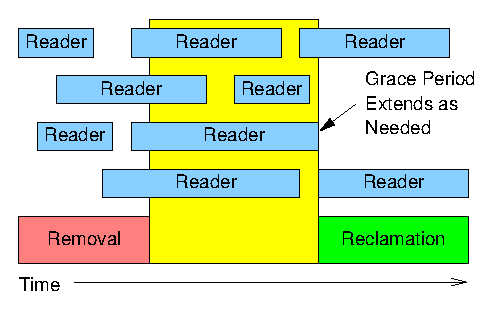
\includegraphics{appendix/rcuimpl/GracePeriodGood}}
\caption{Good Grace Period From Correct RCU}
\label{app:rcuimpl:Good Grace Period From Correct RCU}
\end{figure}

RCU 구현은 이 grace period 를 연장해야 하는데,
Figure~\ref{app:rcuimpl:Good Grace Period From Correct RCU} 에 보여진 것과 같은
형태가 될 수 있겠습니다.
짧게 말해서, 이 RCU 구현은 특정 grace period 의 시작 시점에서 진행 중이던 모든
RCU read-side 크리티컬 섹션은 해당 grace period 가 완료되기 전에 메모리
오퍼레이션들 등의 모든 것이 완전히 종료되었음을 보장해야 합니다.
이 점은 RCU 검증이 집중될 수 있게 해줍니다: 컴파일러나 CPU 가 RCU 구현이 한
일을 무효화 시키는 것을 막도록 충분히 배리어를 써서 하나의 grace period 의 시작
시점에 진행 중이던 RCU read-side 크리티컬 섹션은 모두 해당 grace period 가
종료되기 전에 끝나는 것을  보이는 겁니다.
\iffalse

It must extend the grace period, perhaps as shown in
Figure~\ref{app:rcuimpl:Good Grace Period From Correct RCU}.
In short, the RCU implementation must ensure that any
RCU read-side critical sections in progress at the start of a given grace
period have completely finished, memory operations and all, before that
grace period is permitted to complete.
This fact allows RCU validation to be extremely focused: simply demonstrate
that any RCU read-side critical section in progress at the beginning of
a grace period must terminate before that grace period ends, along with
sufficient barriers to prevent either the compiler or the CPU from undoing
the RCU implementation's work.
\fi

\subsection{Overview of Preemptible RCU Algorithm}
\label{app:rcuimpl:Overview of Preemptible RCU Algorithm}

이 섹션은 preemptible RCU 의 특정 구현에 집중합니다.
많은 다른 구현들이 있을 수 있겠지만, 그에 대해선 다른
곳~\cite{PaulEMcKenney2006b,PaulMcKenney05b} 에서 다루어졌습니다.
이 글은 이 특정 구현의 일반적인 방법들과 데이터 구조, grace-period state
machine, 그리고 read-side 기능들에 대한 파악에 집중합니다.
\iffalse

This section focuses on a specific implementation of preemptible RCU.
Many other implementations are possible, and are described
elsewhere~\cite{PaulEMcKenney2006b,PaulMcKenney05b}.
This article focuses on this specific implementation's
general approach, the data structures,
the grace-period state machine, and a walk through the read-side primitives.
\fi

\subsubsection{General Approach}
\label{app:rcuimpl:General Approach}

\begin{figure}[htb]
\centering
\resizebox{3in}{!}{\includegraphics{appendix/rcuimpl/RCUpreemptListsCompare}}
\caption{Classic vs. Preemptible RCU Callback Processing}
\label{app:rcuimpl:Classic vs. Preemptible RCU Callback Processing}
\end{figure}

이 preemptible RCU 구현은 \co{rcu_read_lock()} 과 \co{rcu_read_unlock()} 에
메모리 배리어를 필요로 하지 않기 때문에, 다단계 grace-period 탐지 알고리즘이
필요합니다.
콜백들을 위한 (기존의 RCU 구현들을 위해선 충분했던) 하나의 \co{wait} queue 를
사용하는 대신에, 이 구현은 \co{wait} 큐들의 배열을 사용해서 RCU 콜백들이 이
배열의 각 원소에 차례차례 enqueue 될 수 있게 합니다.
콜백의 흐름에 있어서의 이 차이가
Figure~\ref{app:rcuimpl:Classic vs. Preemptible RCU Callback Processing}
에 grace period 당 두개의 waitlist stage 들을 갖는 (반면, 2007년 9월 10일의 -rt
로의 패치~\cite{PaulEMcKenney2007PreemptibleRCUPatch} 는 네개의 waitlist stage
를 사용합니다) preemptible RCU 구현에 대해 그려져 있습니다.

Grace period 당 두개의 stage 를 갖기 때문에, 한쌍의 stage 들은 하나의 완전한
grace period 를 구성합니다.
비삿하게, grace period 당 네개의 stage 를 갖는 구현에서는 네개의 stage 의
연속이 하나의 완전한 grace period 를 구성합니다.
\iffalse

Because this implementation of preemptible RCU does not require memory
barriers in \co{rcu_read_lock()} and \co{rcu_read_unlock()},
a multi-stage grace-period detection algorithm is required.
Instead of using a single \co{wait} queue of callbacks
(which has sufficed for earlier RCU implementations), this implementation
uses an array of \co{wait} queues, so that RCU callbacks
are enqueued on each element of this array in turn.
This difference in callback flow is shown in
Figure~\ref{app:rcuimpl:Classic vs. Preemptible RCU Callback Processing}
for a preemptible RCU implementation with two waitlist stages per grace period
(in contrast,
the September 10 2007 patch to -rt~\cite{PaulEMcKenney2007PreemptibleRCUPatch}
uses four waitlist stages).

Given two stages per grace period, any pair of
stages forms a full grace period.
Similarly, in an implementation with four stages per grace period,
any sequence of four stages would form a full grace period.
\fi

\begin{figure}[htb]
\centering
\resizebox{3in}{!}{\includegraphics{appendix/rcuimpl/RCUpreemptCounterFlip}}
\caption{Preemptible RCU Counter Flip Operation}
\label{app:rcuimpl:Preemptible RCU Counter Flip Operation}
\end{figure}

언제 하나의 grace-period stage 가 끝날 수 있는지 판단하기 위해, preemptible RCU
는 진행중인 RCU read-side 크리티컬 섹션들을 추적하는 두개의 원소로 구성된
per-CPU \co{rcu_flipctr} 배열을 사용합니다.
특정 CPU 의 \co{rcu_flipctr} 배열의 하나의 원소는 오래된 RCU read-side 크리티컬
섹션들, 달리 말하자면 현재의 grace-period stage 보다 먼저 시작된 크리티컬
섹션들을 추적합니다.
다른 원소는 새로운 RCU read-side 크리티컬 섹션들을 추적하는데, 이것들은 현재
grace-period stage 중간에 시작된 것들입니다.
이 배열의 원소들은 새로운 grace-period stage 각각의 시작 때마다 그 역할을
바꾸는데,
Figure~\ref{app:rcuimpl:Preemptible RCU Counter Flip Operation} 에 그 모습이
그려져 있습니다.
\iffalse

To determine when a grace-period stage can end,
preemptible RCU uses a per-CPU two-element \co{rcu_flipctr} array
that tracks in-progress RCU read-side critical sections.
One element of a given CPU's \co{rcu_flipctr} array tracks
old RCU read-side critical sections, in other words, critical sections
that started before the current grace-period stage.
The other element tracks new RCU read-side critical
sections, namely those starting during the current grace-period stage.
The array elements switch roles at the beginning of each new grace-period
stage, as shown in
Figure~\ref{app:rcuimpl:Preemptible RCU Counter Flip Operation}.
\fi

앞의 그림의 왼쪽의 첫번째 stage 동안, \co{rcu_flipctr[0]} 는 새로운 RCU
read-side 크리티컬 섹션들을 추적하고, 따라서 \co{rcu_read_lock()} 에 의해 그
값이 증가하고 \co{rcu_read_unlock()} 에 의해 그 값이 감소합니다.
비슷하게, \co{rcu_flipctr[1]} 은 오래된 (앞의 stage 동안 시작된) RCU read-side
크리티컬 섹션들을 추적하고, 따라서 \co{rcu_read_unlock()} 에 의해 그 값이
감소되고 결코 그 값이 증가하지 않습니다.
\iffalse

During the first stage on the left-hand side of the above figure,
\co{rcu_flipctr[0]} tracks the new
RCU read-side critical sections, and is therefore incremented by
\co{rcu_read_lock()} and decremented by \co{rcu_read_unlock()}.
Similarly, \co{rcu_flipctr[1]} tracks the old RCU read-side
critical sections (those that started during earlier stages), and
is therefore decremented by \co{rcu_read_unlock()} and never
incremented at all.
\fi

각 CPU 의 \co{rcu_flipctr[1]} 원소는 결코 그 값이 증가되지 않기 때문에, 모든
CPU 들의 그 원소의 값의 합은 결국은 0이 됩니다, RCU read-side 크리티컬 섹션
중간의 preemption 은 개별적 카운터가 0이 아니게 놔두거나 심지어 음수를 만들
수도 있겠지만 말입니다.
예를 들어, 하나의 task 가 한 CPU 위에서 \co{rcu_read_lock()} 을 호출했고,
preemption 당한 후, 다른 CPU 에서 다시 시작되어서 \co{rcu_read_unlock()} 을
호출했다고 생각해 보세요.
첫번째 CPU 의 카운터는 +1 될것이고 두번째 CPU 의 카운터는 -1 됩니다만, 그 합은
0이 됩니다.
Preemption 의 가능성에 관계 없이, 이 카운터 원소들의 합이 0이 된다면, 앞의
그림의 오른쪽에 보여진 것처럼 다음 grace-period stage 로 넘어가도 안전합니다.
\iffalse

Because each CPU's old \co{rcu_flipctr[1]} elements are never
incremented, their sum across all CPUs must eventually go to zero,
although preemption in the midst of an RCU read-side critical section might
cause any individual counter to remain non-zero or even to go negative.
For example, suppose that a task calls \co{rcu_read_lock()} on
one CPU, is preempted, resumes on another CPU, and then calls
\co{rcu_read_unlock()}.
The first CPU's counter will then be +1 and the second CPU's counter
will be -1, however, they will still sum to zero.
Regardless of possible preemption, when the sum of the old counter
elements does go to zero, it is safe to move to the next grace-period
stage, as shown on the right-hand side of the above figure.
\fi

이 두번째 stage 에서, 각 CPU 의 \co{rcu_flipctr} 카운터 배열의 원소들은 그
역할을 서로 바꿉니다.
\co{rcu_flipctr[0]} 카운터는 이제 오래된 RCU read-side 크리티컬 섹션, 달리 말해
grace period stage 0 동안 시작된 것들을 추적합니다.
비슷하게, \co{rcu_flipctr[1]} 카운터는 이제 grace period stage 1 안에서 시작된
새로운 RCU read-side 크리티컬 섹션들을 추적합니다.
따라서, \co{rcu_read_lock()} 은 이제 \co{rcu_flipctr[1]} 의 값을 증가시키며,
\co{rcu_read_unlock()} 은 여전히 각 카운터의 값을 감소시킵니다.
특히, \co{rcu_read_lock()} 이 grace-period stage 0 (이 시점에선 과거의 stage)
동안 수행되었다면, \co{rcu_read_unlock()} 은 \co{rcu_flipctr[0]} 의 값을
감소시키지만, \co{rcu_read_lock()} 이 grace-period stage 1 (새로운 stage) 동안
수행되었다면, \co{rcu_read_unlock()} 은 \co{rcu_flipctr[1]} 의 값을 감소시켜야
합니다.
\iffalse

In this second stage, the elements of each CPU's \co{rcu_flipctr}
counter array switch roles.
The \co{rcu_flipctr[0]} counter now tracks the old RCU read-side
critical sections, in other words, the ones that started during
grace period stage 0.
Similarly, the \co{rcu_flipctr[1]} counter now tracks the new
RCU read-side critical sections that start in grace period stage 1.
Therefore, \co{rcu_read_lock()} now increments
\co{rcu_flipctr[1]}, while \co{rcu_read_unlock()} still
might decrement either counter.
Specifically, if the matching \co{rcu_read_lock()} executed
during grace-period stage 0 (the old stage at this point), then
\co{rcu_read_unlock()} must decrement \co{rcu_flipctr[0]},
but if the matching \co{rcu_read_lock()} executed during
grace-period stage 1 (the new stage), then \co{rcu_read_unlock()}
must instead decrement \co{rcu_flipctr[1]}.
\fi

여기서의 핵심은 과거의 RCU read-side 크리티컬 섹션들을 추적하는 모든
\co{rcu_flipctr} 원소들이 확실히 감소되어야 한다는 겁니다.
따라서, 일단 이 과거의 것들에 대한 카운터의 합이 0이 된다면, 이는 바뀔 수
없습니다.

\co{rcu_read_lock()} 기능은 \co{rcu_flipctr} 배열을 인덱스 하기 위해 현재
grace-period 카운터의 가장 바닥 bit (\co{rcu_ctrlblk.completed & 0x1}) 을
사용하고, 이 인덱스를 task 구조체 안에 기록해 둡니다.
여기 짝을 맞추는 \co{rcu_read_unlock()} 은 이 기록된 값을 \co{rcu_read_lock()}
이 값 증가시킨 것에 걸맞는 카운터의 값을 감소시킨다는 것을 보장하기 위해
사용합니다.
물론, 이 RCU read-side 크리팈러 섹션이 preemption 당했다면,
\co{rcu_read_unlock()} 은 짝이 맞는 \co{rcu_read_lock()} 이 값을 증가시킨
카운터가 아니라, 다른 CPU 에 속한 카운터의 값을 감소시킬 수도 있습니다.
\iffalse

The critical point is that all \co{rcu_flipctr} elements
tracking the old RCU read-side critical sections must strictly decrease.
Therefore, once the sum of these old counters reaches zero,
it cannot change.

The \co{rcu_read_lock()} primitive uses the bottom
bit of the current grace-period counter
(\co{rcu_ctrlblk.completed & 0x1}) to index the
\co{rcu_flipctr} array,
and records this index in the task structure.
The matching \co{rcu_read_unlock()} uses this recorded
value to ensure that it decrements a counter corresponding to
the one that the matching \co{rcu_read_lock()} incremented.
Of course, if the RCU read-side critical section has been preempted,
\co{rcu_read_unlock()} might be decrementing the counter
belonging to a different CPU than the one whose counter was incremented
by the matching \co{rcu_read_lock()}.
\fi

각각의 CPU 는 또한 \co{rcu_flip_flag} 와 \co{rcu_mb_flag} per-CPU 변수들을 갖고
있습니다.
\co{rcu_flip_flag} 변수는 각 grace-period stage 의 시작을 동기화 시키는 데에
사용됩니다: 일단 특정 CPU 가 \co{rcu_flip_flag} 에 응답했다면, 이제 과거의
grace-period stage 에 연관된 \co{rcu_flip} 배열의 원소의 값을 증가시키는걸
중단해야 합니다.
이 카운터의 값 (\co{rcu_ctrlblk.completed}) 을 증가시키는 CPU 는 각 CPU 의
\co{rcu_mb_flag} 의 값을 \co{rcu_flipped} 로 바꿉니다만, 특정 \co{rcu_mb_flag}
는 연관된 CPU 에 의해서만 \co{rcu_flip_seen} 으로 되바뀔 겁니다.
\iffalse

Each CPU also maintains \co{rcu_flip_flag} and
\co{rcu_mb_flag} per-CPU variables.
The \co{rcu_flip_flag} variable is used to synchronize the
start of each grace-period stage: once a given CPU has responded
to its \co{rcu_flip_flag}, it must refrain from incrementing
the \co{rcu_flip} array element that now corresponds to
the old grace-period stage.
The CPU that advances the counter (\co{rcu_ctrlblk.completed})
changes the value of each CPU's \co{rcu_mb_flag} to
\co{rcu_flipped}, but a given \co{rcu_mb_flag}
may be changed back to \co{rcu_flip_seen} only by
the corresponding CPU.
\fi

\co{rcu_mb_flag} 변수는 각 CPU 가 각 grace-period stage 의 끝에서 메몰
비래이러르 실행하도록 강제하는데에 사용됩니다.
이런 메모리 배리어들은 주어진 grace-period stage 에서 끝나는 RCU read-side
크리티컬 섹션들로부터의 메모리 접근이 이 stage 의 종료 전으로 순서잡힐 것을
보장하는데 필요합니다.
이 방법은 RCU read-side 크리티컬 섹션의 시작과 끝에 비싼 메모리 배리어를 실제로
수행하지 않고도 수행한 것과 같은 효과를 얻게 해줍니다.
\co{rcu_mb_flag} 는 과거의 것들의 카운터의 합이 0이 되는 것을 파악하는 CPU 에
의해 \co{rcu_mb_needed} 로 설정됩니다만, 해당 \co{rcu_mb_flag} 는 연관된 CPU 에
의해서만, 메모리 배리어를 수행한 후에만 \co{rcu_mb_done} 으로 되돌려집니다.
\iffalse

The \co{rcu_mb_flag} variable is used to force each CPU to
execute a memory barrier at the end of each grace-period stage.
These memory barriers are required to ensure that memory accesses from
RCU read-side critical sections ending in a given grace-period stage
are ordered before the end of that stage.
This approach gains the benefits memory barriers at the
beginning and end of each RCU read-side critical section without
having to actually execute all those costly barriers.
The \co{rcu_mb_flag} is set to \co{rcu_mb_needed} by
the CPU that detects that the sum of the old counters is zero,
but a given \co{rcu_mb_flag} is changed back to
\co{rcu_mb_done} only by the corresponding CPU, and even
then only after executing a memory barrier.
\fi

\subsubsection{Data Structures}
\label{app:rcuimpl:Data Structures}

이 섹션은 preemptible RCU 의 주요 데이터 구조인
\co{rcu_ctrlblk}, \co{rcu_data}, \co{rcu_flipctr},
\co{rcu_try_flip_state}, \co{rcu_try_flip_flag}, 그리고
\co{rcu_mb_flag} 를 설명합니다.
\iffalse

This section describes preemptible RCU's major data structures, including
\co{rcu_ctrlblk}, \co{rcu_data}, \co{rcu_flipctr},
\co{rcu_try_flip_state}, \co{rcu_try_flip_flag}, and
\co{rcu_mb_flag}.
\fi

\paragraph{{\tt rcu\_ctrlblk}}
\label{app:rcuimpl:rcu_ctrlblk}

\co{rcu_ctrlblk} 구조체는 전역적으로, grace-period 처리를 보호하는 락
(\co{filplock}) 과 global grace-period 카운터 (\co{completed}) 를 보호하는 락을
잡고 수정됩니다.
\co{completed} 의 가장 아래쪽 bit 은 \co{rcu_read_lock()} 이 어떤 카운터 집합의
값을 증가시킬지 결정하는데 사용됩니다.
\iffalse

The \co{rcu_ctrlblk} structure is global, and holds the lock
that protects grace-period processing (\co{fliplock}) as well
as holding the global grace-period counter (\co{completed}).
The least-significant bit of \co{completed} is used by
\co{rcu_read_lock()} to select which set of counters to increment.
\fi

\paragraph{{\tt rcu\_data}}
\label{app:rcuimpl:rcu_data}

\co{rcu_data} 구조체는 per-CPU 구조체로, 다음과 같은 필드들을 갖습니다:
\iffalse

The \co{rcu_data} structure is a per-CPU structure, and
contains the following fields:
\fi

\begin{itemize}
\item	\co{lock} 은 이 구조체의 나머지 필드들을 보호합니다.
\item	\co{completed} 는 CPU-local 한 활동들을 \co{rcu_ctrlblk} 의 글로벌
	카운터들과 동기화 시키는데에 사용됩니다.
\item	\co{waitlistcount} 는 비어있지 않은 wait-list 의 수를 세는데에
	사용됩니다.
	이 필드는 이 CPU 가 처리해야할 RCU 에 관련된 일을 가지고 있는지
	파악하는걸 돕는데에 \co{rcu_pending()} 에 의해 사용됩니다.
\item	\co{nextlist}, \co{nextail}, \co{waitlist},
	\co{waittail}, \co{donelist}, 그리고
	\co{donetail} 은 grace period 의 종료 시점에 호출되기를 기다리고 있는
	RCU 콜백들로 구성된 리스트들을 형성합니다.
	각각의 리스트는 tail 포인터를 가지고 있어서, $O\left(1\right)$ 삽입을
	허용합니다.
	이 RCU 콜백들은 이 리스트들을 통해 아래에 보여진 것처럼 흘러갑니다.
\item	\co{rcupreempt_trace} 는 통계를 누적합니다.
\iffalse

\item	\co{lock} guards the remaining fields in this structure.
\item	\co{completed} is used to synchronize CPU-local
	activity with the global counter in \co{rcu_ctrlblk}.
\item	\co{waitlistcount} is used to maintain a count of the
	number of non-empty wait-lists.
	This field is used by \co{rcu_pending()} to help determine
	if this CPU has any RCU-related work left to be done.
\item	\co{nextlist}, \co{nextail}, \co{waitlist},
	\co{waittail}, \co{donelist}, and
	\co{donetail} form lists containing
	RCU callbacks that are waiting for invocation at the end
	of a grace period.
	Each list has a tail pointer, allowing $O\left(1\right)$ appends.
	The RCU callbacks flow through these lists as shown below.
\item	\co{rcupreempt_trace} accumulates statistics.
\fi
\end{itemize}

\begin{figure}[htb]
\centering
\resizebox{1.5in}{!}{\includegraphics{appendix/rcuimpl/RCUpreemptLists}}
\caption{Preemptible RCU Callback Flow}
\label{app:rcuimpl:Preemptible RCU Callback Flow}
\end{figure}

Figure~\ref{app:rcuimpl:Preemptible RCU Callback Flow}
는 RCU 콜백들이 \co{rcu_data} 구조체의 리스트들을 \co{call_rcu()} 를 통한
생성부터 \co{rcu_process_callbacks()} 를 통한 호출까지 어떻게 흘러가는지
보입니다.
파란색 화살표는 각각 grace-period state machine 을 통한 이동을 나타내는데, 뒤의
섹션에서 이에 대해 설명합니다.
\iffalse

Figure~\ref{app:rcuimpl:Preemptible RCU Callback Flow}
shows how RCU callbacks flow through a given
\co{rcu_data} structure's lists, from creation by
\co{call_rcu()} through invocation by
\co{rcu_process_callbacks()}.
Each blue arrow represents one pass by the grace-period state machine,
which is described in a later section.
\fi



\paragraph{{\tt rcu\_flipctr}}
\label{app:rcuimpl:rcu_flipctr}

앞에서도 이야기했듯이, \co{rcu_flipctr} per-CPU 카운터 배열은 RCU read-side
크리티컬 섹션들을 추적하는 카운터 쌍들을 담습니다.
이 배열의 어떤 카운터든 음수가 될 수 있는데, 예를 들면 한 task 가 RCU read-side
크리티컬 센션 내에서 다른 CPU 로 옮겨가거나 하는 경우입니다.
하지만, 이 카운터들의 값의 합은 연관된 grace period 동안은 양수로 유지될
것이며, 이 grace period 의 종료 시점에서는 0이 될겁니다.
\iffalse

As noted earlier, the \co{rcu_flipctr}
per-CPU array of counters contains the
counter pairs that track outstanding RCU read-side critical sections.
Any given counter in this array can go negative, for example, when
a task is migrated to a different CPU in the middle of an RCU
read-side critical section.
However, the sum of the counters will
still remain positive throughout the corresponding grace period, and will
furthermore go to zero at the end of that grace period.
\fi

\paragraph{{\tt rcu\_try\_flip\_state}}
\label{app:rcuimpl:rcu_try_flip_state}

\co{rcu_try_flip_state} 변수는 다음 센션에서 설명하는대로 grace-period state
machine 의 현재 상태를 추적합니다.
\iffalse

The \co{rcu_try_flip_state} variable tracks the current state of
the grace-period state machine, as described in the next section.
\fi

\paragraph{{\tt rcu\_try\_flip\_flag}}
\label{app:rcuimpl:rcu_try_flip_flag}

\co{rcu_try_flip_flag} per-CPU 변수는 grace-period 캉누터가 최근에 그 값을
증가시킨데 연관된 CPU 를 알리며 해당 CPU 의 확인을 기록하기도 합니다.
일단 어떤 CPU 가 카운터 뒤집기를 확인하면, 해당 CPU 에서 \co{rcu_read_lock()}
에 의해 취해지는 후속의 동작들은 해당 grace-period 카운터의 새로운 값을 가져야
하는데, 특히 \co{rcu_read_lock()} 내에서 \co{rcu_flipctr} 의 값을 증가시킬 때가
그렇습니다.
\iffalse

The \co{rcu_try_flip_flag} per-CPU variable alerts the corresponding
CPU that the grace-period counter has recently been incremented, and
also records that CPU's acknowledgment.
Once a given CPU has acknowledged the counter flip, all subsequent actions
taken by \co{rcu_read_lock()} on that CPU must account for the
new value of the grace-period counter, in particular, when incrementing
\co{rcu_flipctr} in \co{rcu_read_lock()}.
\fi

\paragraph{{\tt rcu\_mb\_flag}}
\label{app:rcuimpl:rcu_mb_flag}

\co{rcu_mb_flag} per-CPU 변수는 grace-period state machine 이 진행될 수 있도록
하기 위해 메모리 배리어를 반드시 수행해야 하는, 연관된 CPU 를 알리며, 또한 해당
CPU 의 확인을 기록합니다.
일단 어떤 CPU 가 메모리 배리어를 수행하면, RCU read-side 크리티컬 섹션 앞의
모든 메모리 오퍼레이션들은 연관된 grace period 뒤의 코드에 보여질 겁니다.
\iffalse

The \co{rcu_mb_flag} per-CPU variable alerts the corresponding
CPU that it must execute a memory barrier in order for the grace-period
state machine to proceed, and also records that CPU's acknowledgment.
Once a given CPU has executed its memory barrier, the memory operations
of all prior RCU read-side critical will be visible to any code sequenced
after the corresponding grace period.
\fi


\subsubsection{Grace-Period State Machine}
\label{app:rcuimpl:Grace-Period State Machine}

이 섹션은 grace-period state machine 에 의해 수행되는 state 들에 대한 개괄을
제공하고 관련된 코드들을 살펴봅니다.
\iffalse

This section gives an overview of the states executed by the grace-period
state machine, and then walks through the relevant code.
\fi

\paragraph{Grace-Period State Machine Overview}
\label{app:rcuimpl:Grace-Period State Machine Overview}

이 상태 (\co{rcu_try_flip_state} 에 기록되어짐) 는 다음과 같은 값들을 가질 수
있습니다:
\iffalse

The state (recorded in \co{rcu_try_flip_state})
can take on the following values:
\fi

\begin{itemize}
\item	\co{rcu_try_flip_idle_state}:  어떤 RCU grace-period 활동도 없기에
	Grace-period state machine 이 idle 상태에 있음.
	\co{rcu_ctrlblk.completed} grace-period 카운터는 이 상태로부터 빠져나갈
	때마다 값이 증가되고, 모든 per-CPU \co{rcu_flip_flag} 변수들은
	\co{rcu_flipped} 로 설정됩니다.
\item	\co{rcu_try_flip_waitack_state}:
	모든 CPU 들이 각자의 \co{rcu_flip_fflag} 변수를 \co{rcu_flip_seen} 으로
	설정함으로써 기존 state 의 증가를 보았음을 보고하기를 기다리는 상태.
	일단 모든 CPU 들이 이렇게 보고를 하게 되면, 우린 과거의 카운터 집합은
	더이상 값 증가할 수 없음을 알게 됩니다.
\item	\co{rcu_try_flip_waitack_state}:
	기존 카운터들의 값의 합이 0이 되길 기다리는 상태.
	일단 카운터들의 값의 합이 0이 되면, 모든 per-CPU \co{rcu_mb_flag}
	변수들은 \co{rcu_mb_needed} 로 설정됩니다.
\item	\co{rcu_try_flip_waitmb_state}:
	모든 CPU 들이 각자의 \co{rcu_mb_flag} 변수의 값을 \co{rcu_mb_done} 으로
	설정함으로써 메모리 배리어 인스트럭션을 수행했음을 알리기를 기다리는
	상태.
	일단 모든 CPU 들이 메모리 배리어 인스트럭션을 수행하면, 연관된 grace
	period 의 시작 전에 시작된 read-side 크리티컬 섹션에 의해 만들어진
	변경사항은 모든 CPU 들이 볼 수 있을 것임이 완화된 순서규칙의 기계에서도
	보장됩니다.
\iffalse

\item	\co{rcu_try_flip_idle_state}:  the grace-period state
	machine is idle due to there being no RCU grace-period activity.
	The \co{rcu_ctrlblk.completed} grace-period counter
	is incremented upon exit from this state, and all of the
	per-CPU \co{rcu_flip_flag} variables are set
	to \co{rcu_flipped}.
\item	\co{rcu_try_flip_waitack_state}:
	waiting for all CPUs to acknowledge that they have seen the
	previous state's increment, which they do by setting their
	\co{rcu_flip_flag} variables to \co{rcu_flip_seen}.
	Once all CPUs have so acknowledged, we know that the old
	set of counters can no longer be incremented.
\item	\co{rcu_try_flip_waitzero_state}:
	waiting for the old counters to sum to zero.
	Once the counters sum to zero, all of the per-CPU
	\co{rcu_mb_flag} variables are set to
	\co{rcu_mb_needed}.
\item	\co{rcu_try_flip_waitmb_state}:
	waiting for all CPUs to execute a memory-barrier instruction,
	which they signify by setting their \co{rcu_mb_flag}
	variables to \co{rcu_mb_done}.
	Once all CPUs have done so, all CPUs are guaranteed to see
	the changes made by any RCU read-side critical section that
	started before the beginning of the corresponding grace period,
	even on weakly ordered machines.
\fi
\end{itemize}

\begin{figure}[htb]
\centering
\resizebox{3in}{!}{\includegraphics{appendix/rcuimpl/RCUpreemptStates}}
\caption{Preemptible RCU State Machine}
\label{app:rcuimpl:Preemptible RCU State Machine}
\end{figure}

Grace period state machine 은
Figure~\ref{app:rcuimpl:Preemptible RCU State Machine}
에 보여진 것처럼 이 상태들을 순차적으로 돌아갑니다.
\iffalse

The grace period state machine cycles through these states sequentially,
as shown in
Figure~\ref{app:rcuimpl:Preemptible RCU State Machine}.
\fi

\begin{figure}[htb]
\centering
\resizebox{3in}{!}{\includegraphics{appendix/rcuimpl/RCUpreemptTimeline}}
\caption{Preemptible RCU State Machine Timeline}
\label{app:rcuimpl:Preemptible RCU State Machine Timeline}
\end{figure}

Figure~\ref{app:rcuimpl:Preemptible RCU State Machine Timeline}
는 이 state machine 이 어떻게 시간의 흐름에 따라 동작하는지 보입니다.
상태들은 이 그림의 왼쪽에 보여져 있고 연관된 이벤트들이 시간의 흐름에 따라
보여져 있는데, 시간은 아래쪽으로 흐르고 있습니다.
우리는 뒤의 섹션에서 이 알고리즘을 검증할 때에 이 그림을 상세히 설명할 겁니다.

그 전까지는, 여기에 알아둘 중요한 사항들이 있으니 알아두시기 바랍니다:
\iffalse

Figure~\ref{app:rcuimpl:Preemptible RCU State Machine Timeline}
shows how the state machine operates over time.
The states are shown along the figure's left-hand side and the relevant events
are shown along the timeline, with time proceeding in the downward direction.
We will elaborate on this figure when we validate the algorithm in
a later section.

In the meantime, here are some important things to note:
\fi

\begin{enumerate}
\item	\co{rcu_ctrlblk.completed} 카운터의 값 증가는 파란 타원으로 표시된
	것처럼 다른 시간에 다른 CPU 들에 의해 관측되어질 수 있습니다.  하지만,
	해당 CPU 가 이 값 증가를 알아챈 다음에는, 새로운 카운터를 사용해야
	합니다.
	따라서, 일단 모든 CPU 들이 알아챘음을 알린다면, 과거의 카운터의 값은
	감소만 될 수 있습니다.
\item	특정 CPU 는 이 카운터의 값 증가를 알기 전까지만 콜백 리스트들을
	진행시킬 수 있습니다.
\item	파란 타원은 메모리 오퍼레이션 재배치가 다른 CPU 들이 값 증가를 다른
	시간에 볼 수 있음을 알립니다.
	이는 특정 CPU 는 어떤 다른 CPU 가 이 카운터의 새로운 값을 해당 카운터가
	진짜로 증가하기 전에 사용해서 이 구간을 건너뛰었다고 믿을 수도 있음을
	의미합니다.
	실제로, 이론상으로는, 특정 CPU 는 \co{rcu_ctrlblk.completed} 카운터의
	다음의 값 증가를 기존의 메모리 배리어가 쳐진 시점만큼 빠른 시간에
	볼수도 있습니다.
	(이 문장은 매우 부정확함을 알아두시기 바랍니다.
	메모리 배리어에 대한 올바름의 증명을 하고자 한다면,
	Appendix~\ref{app:rcuimpl:Formal Validation} 를 보기 바랍니다.
\iffalse

\item	The increment of the \co{rcu_ctrlblk.completed} counter
	might be observed at different times by different CPUs, as
	indicated by the blue oval.  However, after a given
	CPU has acknowledged the increment, it is required to
	use the new counter.
	Therefore, once all CPUs have acknowledged, the old counter
	can only be decremented.
\item	A given CPU advances its callback lists just before
	acknowledging the counter increment.
\item	The blue oval represents the fact that memory reordering
	might cause different CPUs to see the increment at
	different times.
	This means that a given CPU might believe that some
	other CPU has jumped the gun, using the new value of the counter
	before the counter was actually incremented.
	In fact, in theory, a given CPU might see the next increment of the
	\co{rcu_ctrlblk.completed} counter as early as
	the last preceding memory barrier.
	(Note well that this sentence is very imprecise.
	If you intend to do correctness proofs involving memory barriers,
	please see Appendix~\ref{app:rcuimpl:Formal Validation}.
\fi
\item	\co{rcu_read_lock()} 은 어떤 메모리 배리어도 포함하고 있지 않기 때문에,
	연관된 RCU read-side 크리티컬 섹션들은 해당 CPU 에 의해
	\co{rcu_read_unlock()} 을 뒤따르도록 재배치 될수도 있습니다.
	따라서, 이 RCU read-side 크리티컬 섹션들의 행동들이 실제로 완료되었음을
	보장하기 위해 메모리 배리어가 필요합니다.
\item	이어서 보게 되겠지만, 서로 다른 CPU 들이 카운터의 flip 을 서로 다른
	시간에 볼 수 있다는 사실은 state machine 을 통한 한번의 횡단은 grace
	period 에 충분치 않음을 의미합니다: 여러번의 횡단이 필요합니다.
\iffalse

\item	Because \co{rcu_read_lock()} does not contain any
	memory barriers, the corresponding RCU read-side critical
	sections might be reordered by the CPU to follow the
	\co{rcu_read_unlock()}.
	Therefore, the memory barriers are required to ensure
	that the actions of the RCU read-side critical sections
	have in fact completed.
\item	As we will see, the fact that different CPUs can see the
	counter flip happening at different times means that a
	single trip through the state machine is not sufficient
	for a grace period: multiple trips are required.
\fi
\end{enumerate}

\paragraph{Grace-Period State Machine Walkthrough}
\label{app:rcuimpl:Grace-Period State Machine Walkthrough}

\begin{figure}[tbp]
{ \scriptsize
\begin{verbatim}
  1 void rcu_check_callbacks(int cpu, int user)
  2 {
  3   unsigned long flags;
  4   struct rcu_data *rdp = RCU_DATA_CPU(cpu);
  5
  6   rcu_check_mb(cpu);
  7   if (rcu_ctrlblk.completed == rdp->completed)
  8     rcu_try_flip();
  9   spin_lock_irqsave(&rdp->lock, flags);
 10   RCU_TRACE_RDP(rcupreempt_trace_check_callbacks, rdp);
 11   __rcu_advance_callbacks(rdp);
 12   spin_unlock_irqrestore(&rdp->lock, flags);
 13 }
\end{verbatim}
}
\caption{{\tt rcu\_check\_callbacks()} Implementation}
\label{fig:app:rcuimpl:rcu_check_callbacks() Implementation}
\end{figure}

이 섹션은 scheduling-clock 인터럽트에서 irq (그리고 preemption) 가 비활성화된
채로 \co{rcu_check_callbacks()} 를 호출하는, RCU grace-period state machine 을
구현하는 C 코드를 살펴봅니다.
이 함수는
Figure~\ref{fig:app:rcuimpl:rcu_check_callbacks() Implementation}
에 보여지는 것처럼 구현되어 있습니다.
Line~4 는 현재의 CPU 에 연관된 \co{rcu_data} 구조체를 골라내고 line~6 는 이 CPU
가 state machine 을 \co{rcu_try_flip_waitmb_state} 상태에서 진행시키기 위해
메모리 배리어를 실행해야 하는지를 체크합니다.
Line~7 은 이 CPU 가 이미 현재 grace-period stage number 를 알고 있는지 보고,
그렇다면 line~8 에서 이 state machine 을 진행시킵니다.
Line~9 와 12 는 \co{rcu_data} 의 락을 잡고, line~11 에서는 적절하다면 콜백들을
수행시킵니다.
Line~10 에서는 \co{CONFIG_RCU_TRACE} 가 활성화 되어 있다면 RCU tracing 을 위한
통계들을 업데이트합니다.
\iffalse

This section walks through the C code that implements the RCU
grace-period state machine, which is invoked from the scheduling-clock
interrupt, which invokes \co{rcu_check_callbacks()} with
irqs (and thus also preemption) disabled.
This function is implemented as shown in
Figure~\ref{fig:app:rcuimpl:rcu_check_callbacks() Implementation}.
Line~4 selects the \co{rcu_data} structure corresponding
to the current CPU, and line~6 checks to see if this CPU needs
to execute a memory barrier to advance the state machine out of the
\co{rcu_try_flip_waitmb_state} state.
Line~7 checks to see if this CPU is already aware of the
current grace-period stage number, and line~8 attempts to advance the
state machine if so.
Lines~9 and 12 hold the \co{rcu_data}'s lock, and
line~11 advances callbacks if appropriate.
Line~10 updates RCU tracing statistics, if enabled via
\co{CONFIG_RCU_TRACE}.
\fi

\begin{figure}[tbp]
{ \scriptsize
\begin{verbatim}
  1 static void rcu_check_mb(int cpu)
  2 {
  3   if (per_cpu(rcu_mb_flag, cpu) == rcu_mb_needed) {
  4     smp_mb();
  5     per_cpu(rcu_mb_flag, cpu) = rcu_mb_done;
  6   }
  7 }
\end{verbatim}
}
\caption{{\tt rcu\_check\_mb()} Implementation}
\label{fig:app:rcuimpl:rcu_check_mb() Implementation}
\end{figure}

\co{rcu_check_mb()} 함수는
Figure~\ref{fig:app:rcuimpl:rcu_check_mb() Implementation}
에 보여진 것처럼 필요하면 메모리 배리어를 수행합니다.
Line~3 는 이 CPU 가 메모리 배리어를 수행해야 하는지 체크하고, 만약 그렇다면
line~4 에서 메모리 배리어를 실행하고 line~5 에서 state machine 을 알립니다.
이 메모리 배리어는 \co{rcu_mb_flag} 의 새로운 값을 보는 모든 CPU 는 이 CPU 에
의해 앞의 RCU read-side 크리티컬 섹션 안에서 수행된 메모리 오퍼레이션들을 보게
될 것을 보장함을 알아두시기 바랍니다.
\iffalse

The \co{rcu_check_mb()} function executes a memory barrier
as needed as shown in
Figure~\ref{fig:app:rcuimpl:rcu_check_mb() Implementation}.
Line~3 checks to see if this CPU needs to execute a memory barrier,
and, if so, line~4 executes one and line~5 informs the state
machine.
Note that this memory barrier ensures that any CPU that sees the new
value of \co{rcu_mb_flag} will also see the memory operations
executed by this CPU in any prior RCU read-side critical section.
\fi

\begin{figure}[tbp]
{ \scriptsize
\begin{verbatim}
  1 static void rcu_try_flip(void)
  2 {
  3   unsigned long flags;
  4
  5   RCU_TRACE_ME(rcupreempt_trace_try_flip_1);
  6   if (!spin_trylock_irqsave(&rcu_ctrlblk.fliplock, flags)) {
  7     RCU_TRACE_ME(rcupreempt_trace_try_flip_e1);
  8     return;
  9   }
 10   switch (rcu_try_flip_state) {
 11   case rcu_try_flip_idle_state:
 12     if (rcu_try_flip_idle())
 13       rcu_try_flip_state = rcu_try_flip_waitack_state;
 14     break;
 15   case rcu_try_flip_waitack_state:
 16     if (rcu_try_flip_waitack())
 17       rcu_try_flip_state = rcu_try_flip_waitzero_state;
 18     break;
 19   case rcu_try_flip_waitzero_state:
 20     if (rcu_try_flip_waitzero())
 21       rcu_try_flip_state = rcu_try_flip_waitmb_state;
 22     break;
 23   case rcu_try_flip_waitmb_state:
 24     if (rcu_try_flip_waitmb())
 25       rcu_try_flip_state = rcu_try_flip_idle_state;
 26   }
 27   spin_unlock_irqrestore(&rcu_ctrlblk.fliplock, flags);
 28 }
\end{verbatim}
}
\caption{{\tt rcu\_try\_flip()} Implementation}
\label{fig:app:rcuimpl:rcu_try_flip() Implementation}
\end{figure}

\co{rcu_try_flip()} 함수는
Figure~\ref{fig:app:rcuimpl:rcu_try_flip() Implementation}
에 보인 것처럼 RCU grace-period state machine 의 최고단계 구현을 합니다.
Line~6 는 global RCU state-machine lock 을 획득하려 시도하고, 실패하면
리턴합니다.
Line~5 와 7 은 (\co{CONFIG_RCU_TRACE} 가 활성화 되어 있다면) RCU-tracing 통계를
조작합니다.
Line~10 부터 26 은 state machine 을 수행하는데, 각각 해당 state 에 맞는 함수를
수행시킵니다.
그런 함수 각각은 해당 state 가 진행되야 한다면 1을, 그렇지 않다면 0을
리턴합니다.
원칙적으로, 다음 state 를 곧바로 수행될 수 있지만, 실제로는 응답시간을 줄이기
위해 그렇게 하지 않습니다.
마지막으로, line~27 에서는 line~6 에서 획득했던 global RCU state-machine lock
을 해제합니다.
\iffalse

The \co{rcu_try_flip()} function implements the top level of
the RCU grace-period state machine, as shown in
Figure~\ref{fig:app:rcuimpl:rcu_try_flip() Implementation}.
Line~6 attempts to acquire the global RCU state-machine lock,
and returns if unsuccessful.
Lines;~5 and 7 accumulate RCU-tracing statistics (again, if
\co{CONFIG_RCU_TRACE} is enabled).
Lines~10 through 26 execute the state machine,
each invoking a function specific to that state.
Each such function returns 1 if the state needs to be advanced and
0 otherwise.
In principle, the next state could be executed immediately,
but in practice we choose not to do so in order to reduce latency.
Finally, line~27 releases the global RCU state-machine lock
that was acquired by line~6.
\fi

\begin{figure}[tbp]
{ \scriptsize
\begin{verbatim}
  1 static int rcu_try_flip_idle(void)
  2 {
  3   int cpu;
  4
  5   RCU_TRACE_ME(rcupreempt_trace_try_flip_i1);
  6   if (!rcu_pending(smp_processor_id())) {
  7     RCU_TRACE_ME(rcupreempt_trace_try_flip_ie1);
  8     return 0;
  9   }
 10   RCU_TRACE_ME(rcupreempt_trace_try_flip_g1);
 11   rcu_ctrlblk.completed++;
 12   smp_mb();
 13   for_each_cpu_mask(cpu, rcu_cpu_online_map)
 14     per_cpu(rcu_flip_flag, cpu) = rcu_flipped;
 15   return 1;
 16 }
\end{verbatim}
}
\caption{{\tt rcu\_try\_flip\_idle()} Implementation}
\label{fig:app:rcuimpl:rcu_try_flip_idle() Implementation}
\end{figure}

The \co{rcu_try_flip_idle()} function is called when the
RCU grace-period state machine is idle, and is thus responsible for
getting it started when needed.
Its code is shown in
Figure~\ref{fig:app:rcuimpl:rcu_try_flip_idle() Implementation}.
Line~6 checks to see if there is any RCU grace-period work
pending for this CPU, and if not, line~8 leaves, telling
the top-level state machine to remain in the idle state.
If instead there is work to do, line~11 increments the
grace-period stage counter, line~12 does a memory barrier
to ensure that CPUs see the new counter before they see the
request to acknowledge it, and lines~13 and 14 set all of
the online CPUs' \co{rcu_flip_flag}.
Finally, line~15 tells the top-level state machine to
advance to the next state.

\begin{figure}[tbp]
{ \scriptsize
\begin{verbatim}
  1 static int rcu_try_flip_waitack(void)
  2 {
  3   int cpu;
  4
  5   RCU_TRACE_ME(rcupreempt_trace_try_flip_a1);
  6   for_each_cpu_mask(cpu, rcu_cpu_online_map)
  7     if (per_cpu(rcu_flip_flag, cpu) != rcu_flip_seen) {
  8       RCU_TRACE_ME(rcupreempt_trace_try_flip_ae1);
  9       return 0;
 10     }
 11   smp_mb();
 12   RCU_TRACE_ME(rcupreempt_trace_try_flip_a2);
 13   return 1;
 14 }
\end{verbatim}
}
\caption{{\tt rcu\_try\_flip\_waitack()} Implementation}
\label{fig:app:rcuimpl:rcu_try_flip_waitack() Implementation}
\end{figure}

The \co{rcu_try_flip_waitack()} function, shown in
Figure~\ref{fig:app:rcuimpl:rcu_try_flip_waitack() Implementation},
checks to see
if all online CPUs have acknowledged the counter flip (AKA ``increment'',
but called ``flip'' because the bottom bit, which \co{rcu_read_lock()}
uses to index the \co{rcu_flipctr} array, \emph{does} flip).
If they have, it tells the top-level grace-period state machine to
move to the next state.

Line~6 cycles through all of the online CPUs, and line~7
checks to see if the current such CPU has acknowledged the last counter
flip.
If not, line~9 tells the top-level grace-period state machine to
remain in this state.
Otherwise, if all online CPUs have acknowledged, then line~11
does a memory barrier to ensure that we don't check for zeroes before
the last CPU acknowledges.
This may seem dubious, but CPU designers have sometimes done strange
things.
Finally, line~13 tells the top-level grace-period state machine
to advance to the next state.

\begin{figure}[tbp]
{ \scriptsize
\begin{verbatim}
  1 static int rcu_try_flip_waitzero(void)
  2 {
  3   int cpu;
  4   int lastidx = !(rcu_ctrlblk.completed & 0x1);
  5   int sum = 0;
  6
  7   RCU_TRACE_ME(rcupreempt_trace_try_flip_z1);
  8   for_each_possible_cpu(cpu)
  9     sum += per_cpu(rcu_flipctr, cpu)[lastidx];
 10   if (sum != 0) {
 11     RCU_TRACE_ME(rcupreempt_trace_try_flip_ze1);
 12     return 0;
 13   }
 14   smp_mb();
 15   for_each_cpu_mask(cpu, rcu_cpu_online_map)
 16     per_cpu(rcu_mb_flag, cpu) = rcu_mb_needed;
 17   RCU_TRACE_ME(rcupreempt_trace_try_flip_z2);
 18   return 1;
 19 }
\end{verbatim}
}
\caption{{\tt rcu\_try\_flip\_waitzero()} Implementation}
\label{fig:app:rcuimpl:rcu_try_flip_waitzero() Implementation}
\end{figure}

The \co{rcu_try_flip_waitzero()} function, shown in
Figure~\ref{fig:app:rcuimpl:rcu_try_flip_waitzero() Implementation},
checks to see if
all pre-existing RCU read-side critical sections have completed,
telling the state machine to advance if so.
Lines~8 and 9 sum the counters, and line~10 checks
to see if the result is zero, and, if not, line~12 tells
the state machine to stay right where it is.
Otherwise, line~14 executes a memory barrier to ensure that
no CPU sees the subsequent call for a memory barrier before it
has exited its last RCU read-side critical section.
This possibility might seem remote, but again, CPU designers have
done stranger things, and besides, this is anything but a fastpath.
Lines~15 and 16 set all online CPUs' \co{rcu_mb_flag}
variables, and line~18 tells the state machine to advance to
the next state.

\begin{figure}[tbp]
{ \scriptsize
\begin{verbatim}
  1 static int rcu_try_flip_waitmb(void)
  2 {
  3   int cpu;
  4
  5   RCU_TRACE_ME(rcupreempt_trace_try_flip_m1);
  6   for_each_cpu_mask(cpu, rcu_cpu_online_map)
  7     if (per_cpu(rcu_mb_flag, cpu) != rcu_mb_done) {
  8       RCU_TRACE_ME(rcupreempt_trace_try_flip_me1);
  9       return 0;
 10     }
 11   smp_mb();
 12   RCU_TRACE_ME(rcupreempt_trace_try_flip_m2);
 13   return 1;
 14 }
\end{verbatim}
}
\caption{{\tt rcu\_try\_flip\_waitmb()} Implementation}
\label{fig:app:rcuimpl:rcu_try_flip_waitmb() Implementation}
\end{figure}

The \co{rcu_try_flip_waitmb()} function, shown in
Figure~\ref{fig:app:rcuimpl:rcu_try_flip_waitmb() Implementation},
checks to see
if all online CPUs have executed the requested memory barrier,
telling the state machine to advance if so.
Lines~6 and 7 check each online CPU to see if it has
done the needed memory barrier, and if not, line~9 tells
the state machine not to advance.
Otherwise, if all CPUs have executed a memory barrier, line~11
executes a memory barrier to ensure that any RCU callback invocation
follows all of the memory barriers, and line~13 tells the
state machine to advance.

\begin{figure}[tbp]
{ \scriptsize
\begin{verbatim}
  1 static void __rcu_advance_callbacks(struct rcu_data *rdp)
  2 {
  3   int cpu;
  4   int i;
  5   int wlc = 0;
  6
  7   if (rdp->completed != rcu_ctrlblk.completed) {
  8     if (rdp->waitlist[GP_STAGES - 1] != NULL) {
  9       *rdp->donetail = rdp->waitlist[GP_STAGES - 1];
 10       rdp->donetail = rdp->waittail[GP_STAGES - 1];
 11       RCU_TRACE_RDP(rcupreempt_trace_move2done, rdp);
 12     }
 13     for (i = GP_STAGES - 2; i >= 0; i--) {
 14       if (rdp->waitlist[i] != NULL) {
 15         rdp->waitlist[i + 1] = rdp->waitlist[i];
 16         rdp->waittail[i + 1] = rdp->waittail[i];
 17         wlc++;
 18       } else {
 19         rdp->waitlist[i + 1] = NULL;
 20         rdp->waittail[i + 1] =
 21           &rdp->waitlist[i + 1];
 22       }
 23     }
 24     if (rdp->nextlist != NULL) {
 25       rdp->waitlist[0] = rdp->nextlist;
 26       rdp->waittail[0] = rdp->nexttail;
 27       wlc++;
 28       rdp->nextlist = NULL;
 29       rdp->nexttail = &rdp->nextlist;
 30       RCU_TRACE_RDP(rcupreempt_trace_move2wait, rdp);
 31     } else {
 32       rdp->waitlist[0] = NULL;
 33       rdp->waittail[0] = &rdp->waitlist[0];
 34     }
 35     rdp->waitlistcount = wlc;
 36     rdp->completed = rcu_ctrlblk.completed;
 37   }
 38   cpu = raw_smp_processor_id();
 39   if (per_cpu(rcu_flip_flag, cpu) == rcu_flipped) {
 40     smp_mb();
 41     per_cpu(rcu_flip_flag, cpu) = rcu_flip_seen;
 42     smp_mb();
 43   }
 44 }
\end{verbatim}
}
\caption{{\tt \_\_rcu\_advance\_callbacks()} Implementation}
\label{fig:app:rcuimpl:__rcu_advance_callbacks() Implementation}
\end{figure}

The \co{__rcu_advance_callbacks()} function, shown in
Figure~\ref{fig:app:rcuimpl:__rcu_advance_callbacks() Implementation},
advances callbacks and acknowledges the counter flip.
Line~7 checks to see if the global \co{rcu_ctrlblk.completed}
counter has advanced since the last call by the current CPU to this
function.
If not, callbacks need not be advanced (lines~8-37).
Otherwise, lines~8 through 37 advance callbacks through the lists
(while maintaining a count of the number of non-empty lists in the
\co{wlc} variable).
In either case, lines~38 through 43 acknowledge the counter flip
if needed.

\QuickQuiz{}
	How is it possible for lines~38-43 of
	\co{__rcu_advance_callbacks()} to be executed when
	lines~7-37 have not?
	Won't they both be executed just after a counter flip, and
	never at any other time?
\QuickQuizAnswer{
	Consider the following sequence of events:
	\begin{enumerate}
	\item	CPU 0 executes lines~5-12 of
		\co{rcu_try_flip_idle()}.
	\item	CPU 1 executes \co{__rcu_advance_callbacks()}.
		Because \co{rcu_ctrlblk.completed} has been
		incremented, lines~7-37 execute.
		However, none of the \co{rcu_flip_flag} variables
		have been set, so lines~38-43 do \emph{not} execute.
	\item	CPU 0 executes lines~13-15 of
		\co{rcu_try_flip_idle()}.
	\item	Later, CPU 1 again executes \co{__rcu_advance_callbacks()}.
		The counter has not been incremented since the earlier
		execution, but the \co{rcu_flip_flag} variables have
		all been set, so only lines~38-43 are executed.
	\end{enumerate}
} \QuickQuizEnd


\subsubsection{Read-Side Primitives}
\label{app:rcuimpl:Read-Side Primitives}

This section examines the \co{rcu_read_lock()} and
\co{rcu_read_unlock()} primitives, followed by a
discussion of how this implementation deals with the fact
that these two primitives do not contain memory barriers.

\paragraph{{\tt rcu\_read\_lock()}}
\label{app:rcuimpl:rcu_read_lock()}

\begin{figure}[tbp]
{ \scriptsize
\begin{verbatim}
  1 void __rcu_read_lock(void)
  2 {
  3   int idx;
  4   struct task_struct *t = current;
  5   int nesting;
  6
  7   nesting = ACCESS_ONCE(t->rcu_read_lock_nesting);
  8   if (nesting != 0) {
  9     t->rcu_read_lock_nesting = nesting + 1;
 10   } else {
 11     unsigned long flags;
 12
 13     local_irq_save(flags);
 14     idx = ACCESS_ONCE(rcu_ctrlblk.completed) & 0x1;
 15     ACCESS_ONCE(__get_cpu_var(rcu_flipctr)[idx])++;
 16     ACCESS_ONCE(t->rcu_read_lock_nesting) = nesting + 1;
 17     ACCESS_ONCE(t->rcu_flipctr_idx) = idx;
 18     local_irq_restore(flags);
 19   }
 20 }
\end{verbatim}
}
\caption{{\tt \_\_rcu\_read\_lock()} Implementation}
\label{fig:app:rcuimpl:__rcu_read_lock() Implementation}
\end{figure}

The implementation of \co{rcu_read_lock()} is as shown in
Figure~\ref{fig:app:rcuimpl:__rcu_read_lock() Implementation}.
Line~7 fetches this task's RCU read-side critical-section nesting
counter.
If line~8 finds that this counter is non-zero,
then we are already protected by an outer
\co{rcu_read_lock()}, in which case line~9 simply increments
this counter.

However, if this is the outermost \co{rcu_read_lock()},
then more work is required.
Lines~13 and 18 suppress and restore irqs to ensure that the
intervening code is neither preempted nor interrupted by a
scheduling-clock interrupt (which runs the grace period state machine).
Line~14 fetches the grace-period counter,
line~15 increments the current counter for
this CPU, line~16 increments the nesting counter,
and line~17 records the old/new counter index so that
\co{rcu_read_unlock()} can decrement the corresponding
counter (but on whatever CPU it ends up running on).

The \co{ACCESS_ONCE()} macros force the compiler to
emit the accesses in order.
Although this does not prevent the CPU from reordering the accesses
from the viewpoint of other CPUs, it does ensure that NMI and
SMI handlers running on this CPU will see these accesses in order.
This is critically important:

\begin{enumerate}
\item	In absence of the \co{ACCESS_ONCE()} in the assignment
	to \co{idx}, the compiler would be within its rights
	to: (a) eliminate the local variable \co{idx} and
	(b) compile the increment on line~16 as a
	fetch-increment-store sequence, doing separate accesses to
	\co{rcu_ctrlblk.completed} for the fetch and the
	store.
	If the value of \co{rcu_ctrlblk.completed} had
	changed in the meantime, this would corrupt the
	\co{rcu_flipctr} values.
\item	If the assignment to \co{rcu_read_lock_nesting}
	(line~17) were to be reordered to precede the increment
	of \co{rcu_flipctr} (line~16), and if an
	NMI occurred between these two events, then an
	\co{rcu_read_lock()} in that NMI's handler
	would incorrectly conclude that it was already under the
	protection of \co{rcu_read_lock()}.
\item	If the assignment to \co{rcu_read_lock_nesting}
        (line~17) were to be reordered to follow the assignment
	to \co{rcu_flipctr_idx} (line~18), and if an
	NMI occurred between these two events, then an
	\co{rcu_read_lock()} in that NMI's handler
	would clobber \co{rcu_flipctr_idx}, possibly
	causing the matching \co{rcu_read_unlock()} to
	decrement the wrong counter.
	This in turn could result in premature ending of a
	grace period, indefinite extension of a grace period,
	or even both.
\end{enumerate}

It is not clear that the \co{ACCESS_ONCE} on the assignment to
\co{nesting} (line~7) is required.
It is also unclear whether the \co{smp_read_barrier_depends()}
(line~15) is needed: it was added to ensure that changes to index
and value remain ordered.

The reasons that irqs must be disabled from line~13 through
line~19 are as follows:

\begin{enumerate}
\item	Suppose one CPU loaded \co{rcu_ctrlblk.completed}
	(line~14), then a second CPU incremented this counter,
	and then the first CPU took a scheduling-clock interrupt.
	The first CPU would then see that it needed to acknowledge
	the counter flip, which it would do.
	This acknowledgment is a promise to avoid incrementing
	the newly old counter, and this CPU would break this
	promise.
	Worse yet, this CPU might be preempted immediately upon
	return from the scheduling-clock interrupt, and thus
	end up incrementing the counter at some random point
	in the future.
	Either situation could disrupt grace-period detection.
\item	Disabling irqs has the side effect of disabling preemption.
	If this code were to be preempted between fetching
	\co{rcu_ctrlblk.completed} (line~14) and
	incrementing \co{rcu_flipctr} (line~16),
	it might well be migrated to some other CPU.
	This would result in it non-atomically incrementing
	the counter from that other CPU.
	If this CPU happened to be executing in \co{rcu_read_lock()}
	or \co{rcu_read_unlock()} just at that time, one
	of the increments or decrements might be lost, again
	disrupting grace-period detection.
	The same result could happen on RISC machines if the preemption
	occurred in the middle of the increment (after the fetch of
	the old counter but before the store of the newly incremented
	counter).
\item	Permitting preemption in the midst
	of line~16, between selecting the current CPU's copy
	of the \co{rcu_flipctr} array and the increment of
	the element indicated by \co{rcu_flipctr_idx}, can
	result in a similar failure.
	Execution might well resume on some other CPU.
	If this resumption happened concurrently with an
	\co{rcu_read_lock()} or \co{rcu_read_unlock()}
	running on the original CPU,
	an increment or decrement might be lost, resulting in either
	premature termination of a grace period, indefinite extension
	of a grace period, or even both.
\item	Failing to disable preemption can also defeat RCU priority
	boosting, which relies on \co{rcu_read_lock_nesting}
	to determine when a given task is in an RCU read-side
	critical section.
	So, for example, if a given task is indefinitely
	preempted just after incrementing \co{rcu_flipctr},
	but before updating \co{rcu_read_lock_nesting},
	then it will stall RCU grace periods for as long as it
	is preempted.
	However, because \co{rcu_read_lock_nesting} has not
	yet been incremented, the RCU priority booster has no way
	to tell that boosting is needed.
	Therefore, in the presence of CPU-bound realtime threads,
	the preempted task might stall grace periods indefinitely,
	eventually causing an OOM event.
\end{enumerate}

The last three reasons could of course be addressed by disabling
preemption rather than disabling of irqs, but given that the first
reason requires disabling irqs in any case, there is little reason
to separately disable preemption.
It is entirely possible that the first reason might be tolerated
by requiring an additional grace-period stage, however, it is not
clear that disabling preemption is much faster than disabling
interrupts on modern CPUs.

\paragraph{{\tt rcu\_read\_unlock()}}
\label{app:rcuimpl:rcu_read_unlock()}

\begin{figure}[tbp]
{ \scriptsize
\begin{verbatim}
  1 void __rcu_read_unlock(void)
  2 {
  3   int idx;
  4   struct task_struct *t = current;
  5   int nesting;
  6
  7   nesting = ACCESS_ONCE(t->rcu_read_lock_nesting);
  8   if (nesting > 1) {
  9     t->rcu_read_lock_nesting = nesting - 1;
 10   } else {
 11     unsigned long flags;
 12
 13     local_irq_save(flags);
 14     idx = ACCESS_ONCE(t->rcu_flipctr_idx);
 15     ACCESS_ONCE(t->rcu_read_lock_nesting) = nesting - 1;
 16     ACCESS_ONCE(__get_cpu_var(rcu_flipctr)[idx])--;
 17     local_irq_restore(flags);
 18   }
 19 }
\end{verbatim}
}
\caption{{\tt \_\_rcu\_read\_unlock()} Implementation}
\label{fig:app:rcuimpl:__rcu_read_unlock() Implementation}
\end{figure}

The implementation of \co{rcu_read_unlock()} is shown in
Figure~\ref{fig:app:rcuimpl:__rcu_read_unlock() Implementation}.
Line~7 fetches the \co{rcu_read_lock_nesting} counter,
which line~8 checks to see if we are under the protection of an
enclosing \co{rcu_read_lock()} primitive.
If so, line~9 simply decrements the counter.

However, as with \co{rcu_read_lock()}, we otherwise must do
more work.
Lines~13 and 17 disable and restore irqs in order to prevent
the scheduling-clock interrupt from invoking the grace-period state machine
while in the midst of \co{rcu_read_unlock()} processing.
Line~14 picks up the \co{rcu_flipctr_idx} that was
saved by the matching \co{rcu_read_lock()},
line~15
decrements \co{rcu_read_lock_nesting} so that irq and
NMI/SMI handlers will henceforth update \co{rcu_flipctr},
line~16 decrements the counter (with the same index as, but possibly
on a different CPU than, that incremented by the matching
\co{rcu_read_lock()}.

The \co{ACCESS_ONCE()} macros and irq disabling
are required for similar reasons that they are in
\co{rcu_read_lock()}.

\QuickQuiz{}
	What problems could arise if the lines containing
	\co{ACCESS_ONCE()} in \co{rcu_read_unlock()}
	were reordered by the compiler?
\QuickQuizAnswer{
	\begin{enumerate}
	\item	If the \co{ACCESS_ONCE()} were omitted from the
		fetch of \co{rcu_flipctr_idx} (line~14), then the compiler
		would be within its rights to eliminate \co{idx}.
		It would also be free to compile the \co{rcu_flipctr}
		decrement as a fetch-increment-store sequence, separately
		fetching \co{rcu_flipctr_idx} for both the fetch and
		the store.
		If an NMI were to occur between the fetch and the store, and
		if the NMI handler contained an \co{rcu_read_lock()},
		then the value of \co{rcu_flipctr_idx} would change
		in the meantime, resulting in corruption of the
		\co{rcu_flipctr} values, destroying the ability
		to correctly identify grace periods.
	\item	Another failure that could result from omitting the
		\co{ACCESS_ONCE()} from line~14 is due to
		the compiler reordering this statement to follow the
		decrement of \co{rcu_read_lock_nesting}
		(line~16).
		In this case, if an NMI were to occur between these two
		statements, then any \co{rcu_read_lock()} in the
		NMI handler could corrupt \co{rcu_flipctr_idx},
		causing the wrong \co{rcu_flipctr} to be
		decremented.
		As with the analogous situation in \co{rcu_read_lock()},
		this could result in premature grace-period termination,
		an indefinite grace period, or even both.
	\item	If \co{ACCESS_ONCE()} macros were omitted such that
		the update of \co{rcu_read_lock_nesting} could be
		interchanged by the compiler with the decrement of
		\co{rcu_flipctr}, and if an NMI occurred in between,
		any \co{rcu_read_lock()} in the NMI handler would
		incorrectly conclude that it was protected by an enclosing
		\co{rcu_read_lock()}, and fail to increment the
		\co{rcu_flipctr} variables.
	\end{enumerate}

	It is not clear that the \co{ACCESS_ONCE()} on the
	fetch of \co{rcu_read_lock_nesting} (line~7) is required.
} \QuickQuizEnd

\QuickQuiz{}
	What problems could arise if the lines containing
	\co{ACCESS_ONCE()} in \co{rcu_read_unlock()}
	were reordered by the CPU?
\QuickQuizAnswer{
	Absolutely none!  The code in \co{rcu_read_unlock()}
	interacts with the scheduling-clock interrupt handler
	running on the same CPU, and is thus insensitive to reorderings
	because CPUs always see their own accesses as if they occurred
	in program order.
	Other CPUs do access the \co{rcu_flipctr}, but because these
	other CPUs don't access any of the other variables, ordering is
	irrelevant.
} \QuickQuizEnd

\QuickQuiz{}
	What problems could arise in
	\co{rcu_read_unlock()} if irqs were not disabled?
\QuickQuizAnswer{
	\begin{enumerate}
	\item	Disabling irqs has the side effect of disabling preemption.
		Suppose that this code were to be preempted in the midst
		of line~17 between selecting the current CPU's copy
		of the \co{rcu_flipctr} array and the decrement of
		the element indicated by \co{rcu_flipctr_idx}.
		Execution might well resume on some other CPU.
		If this resumption happened concurrently with an
		\co{rcu_read_lock()} or \co{rcu_read_unlock()}
		running on the original CPU,
		an increment or decrement might be lost, resulting in either
		premature termination of a grace period, indefinite extension
		of a grace period, or even both.
	\item	Failing to disable preemption can also defeat RCU priority
		boosting, which relies on \co{rcu_read_lock_nesting}
		to determine which tasks to boost.
		If preemption occurred between the update of
		\co{rcu_read_lock_nesting} (line~16) and of
		\co{rcu_flipctr} (line~17), then a grace
		period might be stalled until this task resumed.
		But because the RCU priority booster has no way of knowing
		that this particular task is stalling grace periods, needed
		boosting will never occur.
		Therefore, if there are CPU-bound realtime tasks running,
		the preempted task might never resume, stalling grace periods
		indefinitely, and eventually resulting in OOM.
	\end{enumerate}

	Of course, both of these situations could be handled by disabling
	preemption rather than disabling irqs.
	(The CPUs I have access to do not show much difference between these
	two alternatives, but others might.)
} \QuickQuizEnd

\paragraph{Memory-Barrier Considerations}
\label{app:rcuimpl:Memory-Barrier Considerations}

\begin{figure}[htb]
\centering
\resizebox{3in}{!}{\includegraphics{appendix/rcuimpl/RCUrt-MBwaste}}
\caption{Preemptible RCU with Read-Side Memory Barriers}
\label{app:rcuimpl:Preemptible RCU with Read-Side Memory Barriers}
\end{figure}

Note that these two primitives contains no memory barriers, so there is
nothing to stop the CPU from executing the critical section
before executing the \co{rcu_read_lock()} or after executing
the \co{rcu_read_unlock()}.
The purpose of the \co{rcu_try_flip_waitmb_state} is to
account for this possible reordering, but only at the beginning or end of
a grace period.
To see why this approach is helpful, consider
Figure~\ref{app:rcuimpl:Preemptible RCU with Read-Side Memory Barriers},
which shows the wastefulness of the conventional approach of placing
a memory barrier at the beginning and end of each RCU read-side critical
section~\cite{PaulEMcKenney2006b}.

\begin{figure}[htb]
\centering
\resizebox{3in}{!}{\includegraphics{appendix/rcuimpl/RCUrt-MBnowaste}}
\caption{Preemptible RCU with Grace-Period Memory Barriers}
\label{app:rcuimpl:Preemptible RCU with Grace-Period Memory Barriers}
\end{figure}

The ``MB''s represent memory barriers, and only the emboldened
barriers are needed, namely the first and last on a given CPU
for each grace period.
This preemptible RCU implementation therefore associates the memory
barriers with the grace period, as shown in
Figure~\ref{app:rcuimpl:Preemptible RCU with Grace-Period Memory Barriers}.

Given that the Linux kernel can execute literally millions of RCU
read-side critical sections per grace period, this latter approach
can result in substantial read-side savings, due to the fact that it
amortizes the cost of the memory barrier over all the read-side critical
sections in a grace period.

\subsection{Validation of Preemptible RCU}
\label{app:rcuimpl:Validation of Preemptible RCU}

\subsubsection{Testing}
\label{app:rcuimpl:Testing}

The preemptible RCU algorithm was tested with a two-stage grace period
on weakly ordered POWER4 and POWER5 CPUs using rcutorture running for
more than 24 hours on each machine, with 15M and 20M grace periods,
respectively, and with no errors.
Of course, this in no way proves that this algorithm is correct.
At most, it shows either that these two machines were extremely
lucky or that any bugs remaining in preemptible RCU have an extremely
low probability of occurring.
We therefore required additional assurance that this algorithm works,
or, alternatively, identification of remaining bugs.

This task requires a conceptual approach,
which is taken in the next section.

\subsubsection{Conceptual Validation}
\label{app:rcuimpl:Conceptual Validation}

Because neither \co{rcu_read_lock()} nor \co{rcu_read_unlock()}
contain memory barriers, the RCU read-side critical section can bleed
out on weakly ordered machines.
In addition, the relatively loose coupling of this RCU implementation
permits CPUs to disagree on when a given grace period starts and ends.
This leads to the question as to how long a given RCU read-side critical
section can possibly extend relative to the grace-period state machine.

\begin{figure}[htb]
\centering
\resizebox{3in}{!}{\includegraphics{appendix/rcuimpl/RCUpreemptValidation}}
\caption{Preemptible RCU Worst-Case Scenario}
\label{app:rcuimpl:Preemptible RCU Worst-Case Scenario}
\end{figure}

The worst-case scenario is shown in
Figure~\ref{app:rcuimpl:Preemptible RCU Worst-Case Scenario}.
Here, CPU~0 is executing the shortest possible
removal and reclamation sequence,
while CPU~1 executes the longest possible RCU read-side critical
section.
Because the callback queues are advanced just before acknowledging a
counter flip, the latest that CPU~0 can execute its
\co{list_del_rcu()} and \co{call_rcu()} is just before
its scheduling-clock interrupt that acknowledges the counter flip.
The \co{call_rcu()} invocation places the callback on CPU~0's
\co{next} list, and the interrupt will move the callback from
the \co{next} list to the \co{wait[0]} list.
This callback will move again (from the \co{wait[0]} list
to the \co{wait[1]} list) at CPU~0's first scheduling-clock
interrupt following the next counter flip.
Similarly, the callback will move from the \co{wait[1]} list
to the \co{done} list at CPU~0's first scheduling-clock
interrupt following the counter flip resulting in the value 3.
The callback might be invoked immediately afterward.

Meanwhile, CPU~1 is executing an RCU read-side critical section.
Let us assume that the \co{rcu_read_lock()} follows the first
counter flip (the one resulting in the value 1), so that the
\co{rcu_read_lock()} increments CPU~1's
\co{rcu_flipctr[1]} counter.
Note that because \co{rcu_read_lock()} does not contain any
memory barriers, the contents of the critical section might be executed
early by the CPU.
However, this early execution cannot precede the last memory barrier
executed by CPU~1, as shown on the diagram.
This is nevertheless sufficiently early that an \co{rcu_dereference()}
could fetch a pointer to the item being deleted by CPU~0's
\co{list_del_rcu()}.

Because the \co{rcu_read_lock()} incremented an index-1 counter,
the corresponding \co{rcu_read_unlock()} must
precede the ``old counters zero'' event for index 1.
However, because \co{rcu_read_unlock()} contains no memory
barriers, the contents of the corresponding RCU read-side critical
section (possibly including a reference to the item deleted by
CPU~0) can be executed late by CPU~1.
However, it cannot be executed after CPU~1's next memory barrier,
as shown on the diagram.
Because the latest possible reference by CPU~1 precedes the
earliest possible callback invocation by CPU~0, two passes
through the grace-period state machine suffice to constitute
a full grace period, and hence it is safe to do:

\vspace{5pt}
\begin{minipage}[t]{\columnwidth}
\small
\begin{verbatim}
    #define GP_STAGES 2
\end{verbatim}
\end{minipage}
\vspace{5pt}

\QuickQuiz{}
	Suppose that the irq disabling in
	\co{rcu_read_lock()} was replaced by preemption disabling.
	What effect would that have on \co{GP_STAGES}?
\QuickQuizAnswer{
	No finite value of \co{GP_STAGES} suffices.
	The following scenario, courtesy of Oleg Nesterov, demonstrates this:

	Suppose that low-priority Task~A has executed
	\co{rcu_read_lock()} on CPU 0,
	and thus has incremented \co{per_cpu(rcu_flipctr, 0)[0]},
	which thus has a value of one.
	Suppose further that Task~A is now preempted indefinitely.

	Given this situation, consider the following sequence of events:
	\begin{enumerate}
	\item	Task~B starts executing \co{rcu_read_lock()}, also on
		CPU 0, picking up the low-order bit of
		\co{rcu_ctrlblk.completed}, which is still equal to zero.
	\item	Task~B is interrupted by a sufficient number of scheduling-clock
		interrupts to allow the current grace-period stage to complete,
		and also be sufficient long-running interrupts to allow the
		RCU grace-period state machine to advance the
		\co{rcu_ctrlblk.complete} counter so that its bottom bit
		is now equal to one and all CPUs have acknowledged this
		increment operation.
	\item	CPU 1 starts summing the index==0 counters, starting with
		\co{per_cpu(rcu_flipctr, 0)[0]}, which is equal to one
		due to Task~A's increment.
		CPU 1's local variable \co{sum} is therefore equal to one.
	\item	Task~B returns from interrupt, resuming its execution of
		\co{rcu_read_lock()}, incrementing
		\co{per_cpu(rcu_flipctr, 0)[0]}, which now has a value
		of two.
	\item	Task~B is migrated to CPU 2.
	\item	Task~B completes its RCU read-side critical section, and
		executes \co{rcu_read_unlock()}, which decrements
		\co{per_cpu(rcu_flipctr, 2)[0]}, which is now -1.
	\item	CPU 1 now adds \co{per_cpu(rcu_flipctr, 1)[0]} and
		\co{per_cpu(rcu_flipctr, 2)[0]} to its
		local variable \co{sum}, obtaining the value zero.
	\item	CPU 1 then incorrectly concludes that all prior RCU read-side
		critical sections have completed, and advances to the next
		RCU grace-period stage.
		This means that some other task might well free up data
		structures that Task~A is still using!
	\end{enumerate}

	This sequence of events could repeat indefinitely, so that no finite
	value of \co{GP_STAGES} could prevent disrupting Task~A.
	This sequence of events demonstrates the importance of the promise
	made by CPUs that acknowledge an increment of
	\co{rcu_ctrlblk.completed}, as the problem illustrated by the
	above sequence of events is caused by Task~B's repeated failure
	to honor this promise.

	Therefore, more-pervasive changes to the grace-period state will be
	required in order for \co{rcu_read_lock()} to be able to safely
	dispense with irq disabling.
} \QuickQuizEnd

\QuickQuiz{}
	Why can't the \co{rcu_dereference()}
	precede the memory barrier?
\QuickQuizAnswer{
	Because the memory barrier is being executed in
	an interrupt handler, and interrupts are exact in the sense that
	a single value of the PC is saved upon interrupt, so that the
	interrupt occurs at a definite place in the code.
	Therefore, if the
	\co{rcu_dereference()} were to precede the memory barrier,
	the interrupt would have had to have occurred after the
	\co{rcu_dereference()}, and therefore
	the interrupt would also have had to have occurred after the
	\co{rcu_read_lock()} that begins the RCU read-side critical
	section.
	This would have forced the \co{rcu_read_lock()} to use
	the earlier value of the grace-period counter, which would in turn
	have meant that the corresponding \co{rcu_read_unlock()}
	would have had to precede the first ``Old counters zero [0]'' rather
	than the second one.
	This in turn would have meant that the read-side critical section
	would have been much shorter---which would have been
	counter-productive,
	given that the point of this exercise was to identify the longest
	possible RCU read-side critical section.
} \QuickQuizEnd

\subsubsection{Formal Validation}
\label{app:rcuimpl:Formal Validation}

Formal validation of this algorithm is quite important, but remains
as future work.
One tool for doing this validation is described in
Chapter~\ref{chp:Formal Verification}.

\QuickQuiz{}
	What is a more precise way to say ``CPU~0
	might see CPU~1's increment as early as CPU~1's last previous
	memory barrier''?
\QuickQuizAnswer{
	First, it is important to note that the problem with
	the less-precise statement is that it gives the impression that there
	might be a single global timeline, which there is not, at least not for
	popular microprocessors.
	Second, it is important to note that memory barriers are all about
	perceived ordering, not about time.
	Finally, a more precise way of stating above statement would be as
	follows: ``If CPU~0 loads the value resulting from CPU~1's
	increment, then any subsequent load by CPU~0 will see the
	values from any relevant stores by CPU~1 if these stores
	preceded CPU~1's last prior memory barrier.''

	Even this more-precise version leaves some wiggle room.
	The word ``subsequent'' must be understood to mean ``ordered after'',
	either by an explicit memory barrier or by the CPU's underlying
	memory ordering.
	In addition, the memory barriers must be strong enough to order
	the relevant operations.
	For example, CPU~1's last prior memory barrier must order stores
	(for example, \co{smp_wmb()} or \co{smp_mb()}).
	Similarly, if CPU~0 needs an explicit memory barrier to
	ensure that its later load follows the one that saw the increment,
	then this memory barrier needs to be an \co{smp_rmb()}
	or \co{smp_mb()}.

	In general, much care is required when proving parallel algorithms.
} \QuickQuizEnd

